\documentclass[a4paper,12pt,twoside]{book}
\usepackage[utf8]{inputenc}
\usepackage[T1]{fontenc}
\usepackage[greek,english]{babel}
%\usepackage{fontspec}
%\setmainfont[
%  Ligatures=TeX,
%  Extension=.otf,
%  BoldFont=cmunbx,
%  ItalicFont=cmunti,
%  BoldItalicFont=cmunbi,
%  SlantedFont=cmunsl
%]{cmunrm}

%\usepackage{polyglossia}
%\setmainlanguage{spanish}

\usepackage[c5paper]{geometry}
%\geometry{inner=2.5cm,outer=2.5cm,bmargin=3.2cm}
%\usepackage[DIV=14,BCOR=2mm,headinclude=true,footinclude=false]{typearea}

%\usepackage{ulem} %Hace que \emph sea subrayar

%\usepackage[p,osf]{scholax}
%% T1 and textcomp are loaded by package. Change that here, if you want
%% load sans and typewriter packages here, if needed

\usepackage{ebgaramond}
%\usepackage[type1]{libertine} % Linux Libertine for zweispaltige Texte
%\usepackage{textcomp}% Required to get special symbols
\usepackage[scaled=.8]{DejaVuSansMono}% FiraMono Typewriter font
\usepackage{PTSansNarrow} 
%\gilliuscondensed
%\usepackage[sfdefault]{FiraSans}
%\usepackage{bm}% Extra bold faces
%\usepackage[lf]{carlito}

\usepackage{lettrine} %Capital letters at the beginning of a chapter
\usepackage[activate={true,nocompatibility},final,tracking=true,kerning=true,spacing=true,factor=1100,stretch=10,shrink=10]{microtype}
\SetTracking{encoding={*}, shape=sc}{-20} % versalitas menos separadas
% activate={true,nocompatibility} - activate protrusion and expansion
% final - enable microtype; use "draft" to disable
% tracking=true, kerning=true, spacing=true - activate these techniques
% factor=1100 - add 10% to the protrusion amount (default is 1000)
% stretch=10, shrink=10 - reduce stretchability/shrinkability (default is 20/20)

%\usepackage{array,multirow,booktabs,colortbl,chngcntr} % El último es para counterwithout;
\usepackage[strict]{changepage}
%\usepackage{caption}
%\captionsetup{format=plain,labelsep=newline,labelfont={small,sc},
%textfont={small,it},singlelinecheck=false}
\usepackage[Bjornstrup]{fncychap} % Para cabeceras de capítulos sofisticados:     Sonny,    Lenny,    Glenn,    Conny,    Rejne,    and Bjarne.

\usepackage{graphicx,wrapfig,booktabs,multicol,tabularx} % wallpaper: poner imágenes de fondo; wrapfigure: figuras a un lado del texto
%\graphicspath{{figures/}}
\usepackage{fancyhdr}
\usepackage{emptypage,pdfpages,fancybox} % Para que las páginas en blanco no tengan encabezado;
\usepackage{enumitem} %paralist: para compactenum, enumerate sin espacios
%\setlist[itemize]{nosep} %Espacio entre items en itemize
\usepackage[hyperref]{xcolor}
\usepackage[hidelinks]{hyperref}
\usepackage{xurl}
\usepackage{verse}
\usepackage{paracol}
\usepackage{longtable}
\usepackage{CJKutf8}

%\usepackage{minipage}

%\usepackage{quotchap} %Encabezados de capítulos
\usepackage{syntonly,verbatim}
%\syntaxonly

\usepackage{setspace,xspace} % xspace: Da \xspace para no tener que poner {} después de los comandos; pdflscape: páginas en horizontal;

\newenvironment{quotex}{\begin{quote}\small}{\end{quote}}
\newenvironment{quotationx}{\begin{quotation}\small}{\end{quotation}}


\begin{document}

% Por alguna razón, los marginados se creaban al revés. Así los corrijo. Feo, pero eficaz:
\let\tmp\oddsidemargin
\let\oddsidemargin\evensidemargin
\let\evensidemargin\tmp
\reversemarginpar

%\setcounter{secnumdepth}{4} % Para que llegue a numerar hasta las subsubsecciones;
%\renewcommand{\heavyrulewidth}{0.14em} % Grosor de las líneas extremas de las tablas;
%\renewcommand\thempfootnote{\alpha{mpfootnote}} % Símbolo de notas dentro de minipage
%\let\oldcaptionof\captionof
%\renewcommand{\captionof}[2]{\oldcaptionof{#1}{\newline \textit{#2} }}
%\renewcommand{\tablename}{Tabla}
%\counterwithout{figure}{chapter}
%\counterwithout{table}{chapter} % Así la numeración es 1, 2, 3... y no 1.1, 1.2... y no reinicia la num. en cada capítulo;

%\providecommand{\ggl}{\guillemotleft}
%\providecommand{\ggr}{\guillemotright\xspace}
\providecommand{\flright}[1]{\begin{flushright}#1\end{flushright}}
\providecommand{\flrightit}[1]{\begin{flushright}\itshape #1\end{flushright}}
%\renewcommand\UrlFont\sffamily
\urlstyle{tt}

\pagestyle{fancy}
\renewcommand{\sectionmark}[1]{\markright{#1}}
\renewcommand{\chaptermark}[1]{\markboth{#1}{}}

%Portada:
%\includepdf{00Portada}

\frontmatter
%
%\onehalfspacing
%\pagenumbering{Roman} %gobble es como empty

%\include{preindice}

%\fancyhf{}
%\fancyhead[LE]{\small \textbf{\thepage}$\quad$ Índice general}
%\fancyhead[RO]{\small Índice general $\quad$\textbf{\thepage}}
%\clearpage
\tableofcontents

%\doublespacing
\mainmatter

\fancyhf{}
\fancyhead[LE]{\small \thepage$\quad${\scshape\chaptername{} \thechapter}: \nouppercase{\itshape\leftmark}}
\fancyhead[RO]{\small \textsc{Section }\thesection{}: \nouppercase{\itshape\rightmark} $\quad$\upshape\thepage}
%\cfoot{\bfseries\thepage}

\pagenumbering{arabic}

%\onehalfspacing

% introductorios
\chapter{Posts by Logres}
\section{Transformational Possibilities}

\begin{quotex}
Gornahoor would like to welcome Logres who will be posting articles on Fridays for the next several weeks as I take time to pursue other interests. 
\flright{\textsc{Cologero}}
\end{quotex}

The default fundamentalism inherent in so much of contemporary American or even Western Christianity is a cause of some dismay for traditionalists who yearn to look into this tradition for inspiration and support. Watching modern Christians flail their way into movements like the emergent Church\footnote{\url{https://en.wikipedia.org/wiki/Emerging\_church}} or Radical Orthodoxy\footnote{\url{https://en.wikipedia.org/wiki/Radical\_Orthodoxy}} is frustrating or even infuriating. How can so much well-meaning and almost-right energy be spent in ignoring the deeper cultural connections also inherent in the Faith? Any moment, now, one feels that the thrashing may re-ignite the genuine article almost by accident.

Many critics have argued persuasively that Christianity is inherently ``Judaizing'' and doomed to repeat the innate short-circuits infused within the various cultural patterns it assimilated on its path to ascendancy, and they are invariably helped on by some theologians who actually sing paeans of praise.

Specifically, the literalism of the Scriptures as a Holy Book seem to be a fundamental limiting pattern within dialogue on this subject, within and without the Faith. The supposedly perspicacious Writ is quoted against and for us, designedly to limit certain possibilities and force others, usually something compatible with a global universal political settlement.

To these, one might quote Luther, ``The letter is poison.'' (Schrift ist gift). Obviously, this dichotomy set up in the New Testament is a vehicle for higher purpose, and was a major complaint of Jews against Christians, not without reason. To the Biblical narrative, the traditionalist can bring a deeper awareness of unnoticed patterns heretofore ignored. There is, of course, the great solar tradition hidden within the Davidic dynasty, inaugurated when King David opened the inner sanctuary and ate of the shewbread upon the holy mount of peace, a holy site from very ancient times. Troy Southgate's uneven website drew attention to this, in an article by Bill White\footnote{\url{http://www.rosenoire.org/articles/aryan.php}}. It wasn't as if King David was following the letter of the Law in piercing the veil, and he probably didn't have a rope tied to his leg just in case a burial was needed. The order of Melchizedek was another ancient order connected with Salem, and there is also the strange episode of Namaan bowing down in the temple of Rimmon at the advice of Elijah.

Add to this the strange verses in Paul's writings about ``tutelary spirits'' raising the consciousness of nations, baptism for the dead, and the theory of recapitulation of the All through the Kingship-Headship of Christ, as well as parallelisms that exist between many of Christ's saying and the Vedantic\footnote{\url{http://www.biblicalstudies.org.uk/pdf/ijt/30-1_024.pdf}} tradition, as well as the imagery of Revelation, and the Scriptures could begin to look far more interesting. Ask most Christians what Christ meant when he said each little one had a guardian spirit that beholds the face of the Father directly, and you will be met with utter incomprehension or disbelief. We may dismiss their good opinion and proceed. Yet we need not concede them control over the vehicles, since to do so strips our effort of needful road signs or tools.

For example, the Christian Reconstructionist James Jordan\footnote{\url{http://www.biblicalhorizons.com/pdf/jjne.pdf}} has written an obscure but useful book about the hidden symbols of the Bible that are in plain sight, and Jonathan Edwards (had he lived) might have greatly developed his portrayal of the Platonic\footnote{\url{http://www.jesociety.org/2011/02/10/was-jonathan-edwards-a-gnostic/}} imagery of nature\footnote{\url{http://www.ts.mu.edu/content/65/65.1/65.1.3.pdf}}. Is it an accident that men like Marsilio Ficino pop up within Western streams of thought and religion, \emph{or is it wholly for our sake, for the Now, that they wrote what they wrote}? \emph{To cleanse the doors of perception for the I which aspires in the Now for truth, but has lost its way}? In the dearth of a true tradition, Christians (and those who would use the vehicle as they may) are compelled to re-forge the sword which was broken -- we cannot look to the official institutions themselves for confirmation, aid, or blessing.

To those false sons within the pale, and those who scorn the true Church as utterly bereft of real grace, we ought to reply with Isaac Penington, and apply this unction to the dying Faith:

\begin{quotex}
Every truth is a shadow except the last. But every truth is substance in its own place, though it be but a shadow in another. And the shadow is a true shadow, as the substance is a true substance.
\end{quotex}


These fragments of truth which she has grasped, like some \emph{de copia} of Erasmus, she has shored against her ``ruin''. The work will begin. We will make our inheritance our own, and the letter shall be burned.


\flrightit{Posted on 2011-04-08 by Logres}

\begin{center}* * *\end{center}

\begin{footnotesize}
\begin{sffamily}
\texttt{Spock on 2011-04-08 at 09:13 said:}

Biblical passages don't prove much of anything, only that the scribes or forgers could copy from other manuscripts.

\hfill

\texttt{Cologero on 2011-04-08 at 12:56 said:}

There are some defects in the James Jordan text, particularly in his understanding of the ``creation'' of the world. He takes the position that God could have created any possible world, where by ``possible'' he means any world that James Jordan can conceive in his imagination. However, there is no reason to suppose that whatever James Jordan can imagine is actually realizable. That may be the Jewish interpretation, but it is not the Christian.

Christian understanding states that everything was created through the Logos: ``All things were made by him Logos; and without him was not any thing made that was made.''

So when James Jordan wonders why the world is the way it is, that is because it conforms to a cosmic order, a topic we have addressed many times. As far as Mr. Jordan's objection to Plato, we can assure him that it was John himself who made the connection to the Logos of Greek philosophy. The Alexandrians and Augustine just noted it and drew out the consequences.

\hfill

\texttt{logres on 2011-04-08 at 20:58 said:}

Thanks for pointing that out by articulating it clearly; that's the problem with many branches of Christian tradition, and one I know very personally -- one has a naive faith, then it is ``lost'', and/or one comes upon a writer like Jordan who does dip into the pool a little bit, leaving one with the general idea that all has been said. Whereupon, one shuts one's self off from any further development. In Jordan's case, he's just more interesting than the average theologian, and therefore more helpful and dangerous all at once. Such debates do represent a possible apologetic angle for traditionalists, as Cologero has outlined. And thanks for the welcome.

\hfill

\texttt{Ismo Meinander on 2011-04-09 at 05:29 said:}

Cologero said: Christian understanding states that everything was created through the Logos: ``All things were made by him Logos; and without him was not any thing made that was made.''

There is a very interesting passage in Wolfgang Smith's `The Quantum Enigma' concerning this biblical quotation, in which he discusses the issue of causation and vertical causality in the context of art and creativity. I think it is best for me to quote him straight from the book:

``It emerges that there exists a primary causality which acts, not in some distant past, but in every here and now without exception. All things existing in space and time are not only brought into being, but held in existence, byt this primary causation which derives from a single and indivisible Act. Unlike the kinds of causality with which modern science is concerned -- which may be termed temporal or natural causation -- this primary causality does not act from past to futur by way of a temporary process, but acts directly, unmediated by any chain of temporal events. The question arises now whether this `temporally unmediated' mode of action -- which we shall designate by the adjective vertical -- is the exclusive prerogative of primary causation, or whether perhaps there exist secondary modes of vertical causality. In answer to this question it can be said that the causation effected by an intelligent agent is perforce vertical. Take the case of art in the primitive sence of human making: the entire process hinges in fact upon such a vertical act. What stands at issue in authentic art is a veritable imitatio Dei: the human artist `participates' to some degree in the creative process of the First Cause: `All things were made by Him, and without Him not anything was made' (John 1: 13). But does this mean that all production -- even the shoddiest artifact -- is to be ascribed indisriminately to God Himself? Assuredly not. It is interesting to note, in this connection, that according to the punctuation which became generally accepted in post-medievval times, John 1: 13 actually reads: `All things were made by Him, and without Him was not anything made that was truly made.'' We may take it that the quod factum est refers to what is truly made, and therefore what truly is. The difference, Scholastically speaking, lies in the presence or absence of form: it is form -- a transcendent element! -- that bestows being. Now, the bestowal of form constitues an incurably vertical act of causation.''

So I take it that `vertical causation' is another way of expressing the `eternal now' and in reference to the `creation' it can be said that the world is created by the immanently transcendent divinity anew from moment to moment. So the passage could go also `everything is created by Him and without Him nothing is made that is truly made. I think this conception of `an eternal creation' should be emphasized and elaborted every time when one speaks for example with scientists about `the creation of the world' and the world process: The Primary Act did not act in `the big bang' and then evade itself in some transcendent dimension of Being like the Deists seem to think, but it acts in everything, especially and in potentia conscously through humans who have the possibilities to conceive it unlike animals and non-human Nature that follows its ways instinctually, and nothing could not exist without this immanent participation into the higher states of being either consciously or un-consciously. In the realm of art and human creativity it can be said that true art in some way or another reflects harmoniously the intellect of the Logos.

\hfill

\texttt{Ismo Meinander on 2011-04-09 at 05:40 said:}

Correction: `... and nothing could not exist... ' -- `nothing could exist'. My english is not perfect \& I apologize some possible mistakes.

\hfill

\texttt{Cologero on 2011-04-09 at 19:13 said:}

Thanks for pointing out that passage from Wolfgang Smith. It ties in, too, with Mouravieff's New Age, the era of the Artist ... as you and Prof Smith use the term. Artistic intuition needs to be expressed, and artistic expression is a continuing creative process, not a once and for all times event.

\hfill

\texttt{Cologero on 2011-04-09 at 19:32 said:}

By attempting to recover the symbolic, Jordan is accidentally interesting but he ruins it with his literalness and fundamentalism. As an example, we can point to his misunderstanding of the cosmology of the four elements as a sort of proto-chemistry in the modern sense. Of course not, but as a qualitative understanding of the world, it is adequate and accurate. Could God have created a world without one of the four qualitative elements? Perhaps a world without the liquid state (water)? Inconceivable. Or without energy (fire)? Not at all. God is arbitrary for Jordan, not consubstantial with the Logos.

\hfill

\texttt{logres on 2011-04-10 at 00:49 said:}

Yes, I hadn't thought deeply enough about the why of Jordan being wrong, but ``accidentally interesting'' probably aptly characterizes his work. I read a Catholic writer who thought that Duns Scotus' emphasis on God's will lead to problems in the West, but as I've come across traditionalist writers, I see that even this doesn't get deep enough. The examples are endless: Richard Weaver blaming William of Occam in Ideas Have Consequences, etc., etc. A lot of blaming in the West, not much substance, or rather, not enough to warrant a prophetic tone. Harold Weatherby has an interesting book called ``The Keen Delight'' on the effect of bad philosophy on poetry. He starts with Dante, goes through Hopkins, and ends with Eliot. Of course, his answer is more ``scholasticism'' of the Aquinas-type.

\hfill

\end{sffamily}
\end{footnotesize}


\section{Titus Flavius Clemens and the Golden Chain}

What evidence could we adduce for the claim that Clement of Alexandria possessed secret wisdom?

First of all, we could establish his difference from (say) Tertullian or even Jerome (who had the dream about getting rid of his pagan library):

\begin{quotex}
... by philosophy I mean not the Stoic, nor the Platonic, nor the Epicurean, nor that of Aristotle; but whatever any of these sects had said that was fit and just, that taught righteousness with a divine and religious knowledge, this I call eclectic philosophy.
\end{quotex}


For Clement, Christianity was true, not because it overthrew paganism, but because it completed it. Furthermore, truth was truth, not ``Christian'' truth. Yet he goes somewhat further, differing from (say) Augustine, who first believed in order to understand, writing instead that

\begin{quotex}
As many men drawing down the ship, cannot be called many causes, but one cause consisting of many; --- for each individual by himself is not the cause of the ship being drawn, but along with the rest; --- so also philosophy, being the search for truth, contributes to the comprehension of truth; \textbf{not as being the cause of comprehension, but a cause along with other things, and co-operator; perhaps also a joint cause}. ... But the Hellenic truth is distinct from that held by us (although it has got the same name), both in respect of extent of knowledge, certainly of demonstration, divine power, and the like. For we are taught of God, being instructed in the truly ``sacred letters'' by the Son of God. \textbf{Whence those, to whom we refer, influence souls not in the way we do, but by different teaching.} And if, for the sake of those who are fond of fault-finding, we must draw a distinction, by saying that philosophy is a concurrent and cooperating cause of true apprehension, being the search for truth, then we shall avow it to be a preparatory training for the enlightened man (\emph{to gnostikon}); not assigning as the cause that which is but the joint-cause; nor as the upholding cause, what is merely co-operative; \emph{nor giving to philosophy the place of a sine qua non.} Since almost all of us, without training in arts and sciences, and the Hellenic philosophy, and some even without learning at all, through the influence of a philosophy divine and barbarous, and by power, have through faith received the word concerning God, \textbf{trained by self-operating wisdom}. But that which acts in conjunction with something else, being of itself incapable of operating by itself, we describe as co-operating and concausing, and say that it becomes a cause only in virtue of its being a joint-cause, and receives the name of cause only in respect of its concurring with something else, but that it cannot by itself produce the right effect.
\end{quotex}


The reserve about ``sine qua non'' is perhaps worth further debate. However, one understands, in order to believe. Yet one might go (in fact) further than this and construe that for Clement, Christianity could only remain true to the extent that it was also willing to be completed in its turn, or re-completed. That is, what took absolute precedence over exoteric doctrine would have been the divine Logos which from the beginning undertook the creation of the world as a school for the souls of men, a school which was living and active, creative and artful, not capable of being uttered in fullness in a creed. This plan would have been understood as articulated (and articulate) through initiation into what was pellucid, beautiful, and virtuous, the vestibules of the holy. ``He who finds them, finds more.'' The mastery of such would have been gnosis, the goal of pistis (only in this sense inseparable, but absolutely separate otherwise, since Clement would never have separated pistis completely from gnosis, but defended the ``higher knowledge''):

\begin{quotex}
It is then, as appears, the greatest of all lessons to know one's self. For if one know himself, he will know God; and knowing God, he will be made like God... But that man with whom the Word dwells does not alter himself, does not get himself up: he has the form which is of the Word; he is made like to God... and that man becomes God, since God so wills. Heraclitus, then, rightly said, ``Men are gods, and gods are men.'' (ANF 2.271). \flright{\emph{The Instructor}, 3.1}

On this wise it is possible for the true Gnostic already to have become God. ``I said, Ye are gods, and sons of the highest.'' (ANF 2.437). \flright{\emph{Strom.}, 4.23}

By thus receiving the Lord's power, the soul studies to be God; ... To the likeness of God, then, he that is introduced into adoption and the friendship of God, to the just inheritance of the lords and gods is brought; if he be perfected, according to the Gospel, as the Lord himself taught. (ANF 2.506) \flright{\emph{Strom.}, 6.14}

... they are called by the appellation of gods, being destined to sit on thrones with the other gods that have been first put in their places by the Saviour. (ANF 2.539). \flright{\emph{Strom.}, 7.10}

What, then, shall we say of the true Gnostic himself? ``Know ye not'', says the apostle, ``that ye are the temple of God?'' The true Gnostic is consequently divine, and already holy, God-bearing and God-borne. (ANF 2.547). \flright{\emph{Strom.}, 7.13}

But he who has returned from this deception, on hearing the Scriptures, and turned his life to the truth, is, as it were, from being a man made a god. (ANF 2.551) \flright{\emph{Strom.}, 7.16}
\end{quotex}


Yet there is even more than demonstrating the fitness of Clement's teaching as a vessel for esotericism. Although the Mar Saba letter of Clement mentioning the ``secret Gospel of Mark'' is debated among scholars, we should not be entirely convinced by scholars who argue\footnote{\url{http://ixoyc.net/data/Fathers/622.pdf}} that Clement's lack of further quotation implies disapproval.

Clement himself held a position that truth was incommunicable at high levels, except by initiation, or proper coding. This is consistent with his Pythagoreanism\footnote{\url{http://www.bu.edu/wcp/Papers/Anci/AnciAfon.htm}}.

This is drawn out at length by S. Muller\footnote{\url{http://stephanhuller.blogspot.com/2011/01/how-to-read-and-understand-clement-of_23.html}}:

\begin{quotationx}
As we noted in our last post Clement used the conflict with regards to Paul accepting circumcision in Acts and the Epistle to the Galatians to illustrate `a hidden harmony' which is necessary for `right conduct' and `right belief.' Now Clement has moved beyond this and opened the door to things written in two different forms in two different `forms' of the gospel. What Jesus spoke in a low voice (whispered) are the parables which appear in the revealed gospels of Christianity which circulate generally. These parables represent a `lower' or subordinate form of the mystic wisdom ultimately revealed by Jesus and preserved in some other gospel form. Yet the harmony between these two gospel forms is indeed what Clement understands as the `ecclesiastic canon' -- a Pythagorean term which clearly represents again the preserving of an original tune in a `lower key' (perhaps distinguished from the tonic by a ``\emph{diatessaron}''). 

When we go back to Clement's original discussion it is important to see the underlying Pythagorean coloring to his use of the term \emph{kanona}. For we read again: ``He spake all things in parables, and without a parable spake He nothing unto them;'' and if ``all things were made by Him, and without Him was not anything made that was made,'' consequently also prophecy and the law were by Him, and were spoken by Him in parables. ``But all things are right,'' says the Scripture, ``before those who understand,'' that is, those who receive and observe, according to the exposition of the Scriptures explained by Him according to the ecclesiastic canon; and the ecclesiastical rule is the concord and harmony of the law and the prophets in the covenant delivered at the coming of the Lord.

Thus in no uncertain terms then, Clement understands the term `canon' in a Pythagorean sense. In this particular case Clement uses Jesus's condemnation of the Pharisees who `lie' about the truth of the Law and the prophets and its prediction of a messiah like Christ as an example of unworthy behavior in the temporary Alexandrian community. Whoever Clement is attacking (the Carpocratians? the Marcionites? both?) have divorced the secret gospel from its original `harmony' with the public gospels so as to ruin the true ecclesiastic `canon' understood in the Pythagorean sense.
\end{quotationx}


Salvatore Lilla\footnote{\url{http://journals.cambridge.org/action/displayAbstract;jsessionid=C80CC407F4BFC4A35AD9963BC675DA26.tomcat1?fromPage=online\&aid=2407972}} is agreed to have done good work on Clement explicitly in relation to the Gnostics, which dimension of Clement had been previously ignored (perhaps because there are so many others?).

The body of Clement's work is saturated (also) with Jewish\footnote{\url{http://www.bgbucur.com/PDFuri/ClementHierarchy.pdf}} mythology.

It is unnecessary to rehearse his spiritual lineage through Papias to the apostles, or to trace his influence in later Church mystical theology, but Dionysius was an indirect pupil, and Dionysius' writings are arguably ``unorthodox'' enough to accommodate a possible Hermetic root source. The notion of the deep ``I'' emanating and proceeding and then returning\footnote{\url{http://www.reversespins.com/dionysius.html}} to God are of particular import. His Stoical influences are so far beyond doubt as to be unremarkable.

We can conclude that Clement's ``canon'' included all things because ``all things were from God''. Thus, paganism cannot evaporate or be subordinated:

\begin{quotex}
In fact, nevertheless the thief possesses really, what he has possessed himself of dishonestly, whether it be gold, or silver, or speech, or dogma. The ideas, then, which they have stolen, and which are partially true, they know by conjecture and necessary logical deduction: on becoming disciples, therefore, they will know them with intelligent apprehension.
\end{quotex}


Here, Clement virtually argues that Christian Gnosis in fact re-illuminates that which it has already illuminated indirectly, through union with its derivatives. This return and reconciliation (similar to the doctrine of recapitulation given in Colossians) of paganism and Christianity should make clear that it was possible to achieve a balance between the two which allowed ``each to be for the other, but differently''.

Clement himself admitted that there was a ``secret Gospel'', but claimed that it was not what the Gnostics pretended it to be. Might it have looked more like Mouravieff's\footnote{\url{http://www.bibliotecapleyades.net/archivos_pdf/mouravieff3.pdf}} work?

Even his pupil Origen's echo is true to this presupposition \& Clement's teaching:

\begin{quotex}
Jesus conversed with His disciples in private, and especially in their sacred retreats, concerning the Gospel of God; but the words which He uttered have not been preserved, because it appeared to the evangelists that they could not be adequately conveyed to the multitude in writing or in speech... and they saw... what things were to be committed to writing, and how this was to be done, and what was by no means to be written to the multitude, and what was to be expressed in words, and what was not to be so conveyed. \flright{\textit{Contra Celsus}, VI, 18}
\end{quotex}


So that Clement's citation of Paul's words make perfect sense:

\begin{quotex}
Take also the Hellenic books, read the Sibyl, how it is shown that God is one, and how the future is indicated. \flright{\textsc{Clement}, \textit{Stromata}, Book VI, chap. VII}
\end{quotex}


God is one, truth is one. It should be clear by now that Titus Flavius Clemen's thought-world (still very similar to St. Paul's) was a far cry from that of Tertullian, Cyprian, Iranaeus, or even Augustine, and that the Latin world's loss of the Alexandrian library was a very symbolic event. Clement seems to have been a point of intersection for an amazing amount of eclectic influence, and it would be very surprising if that were merely a matter of chance.


\flrightit{Posted on 2011-04-15 by Logres}

\begin{center}* * *\end{center}

\begin{footnotesize}
\begin{sffamily}

\texttt{Logres on 2011-04-16 at 11:16 said:}

Clement is not arguing at all that Christianity ``saved'' paganism -- that is an Augustinian argument.

\hfill

\texttt{Spock on 2011-04-17 at 10:03 said:}

Whether completed or saved is splitting hairs. My reference to saving was to the gentiles not to paganism where I used Clement's word ``completing.'' However, salvation and completion you must admit carry an almost identical value.

\hfill

\texttt{Logres on 2011-04-17 at 19:35 said:}

Spock, they could mean the same thing, but Clement's ``mental and spiritual furniture'' indicate they don't. Clement does not think that the Gospel ``saves'' the pagan schools. And it completes them only by essentially being the same thing, \textbf{except more so}.

It might be worth while pondering the effect Augustine and his milieu had on the infant Church. Although I might be willing to concede that Saint Paul comes down on the side of ``Platonism for the masses'' (not my original phrase), at least in general effect, it seems clear that the collapse of the Empire, the persecutions (which annihilated true apostolic succession in a lineal sense), and the general confusion of the Late Roman period combined to form in Saint Augustine a decisive favoring of Latinate ``City of God'' style religion as opposed to authentic and alternate streams present in the Church, which were still there as late as Boethius. Even the Orthodox want to credit Augustine here, for his insistence (echoed today by V. Lossky, the premier mystical theologian)that there is no such thing as ``hidden'' wisdom apart from dogma. Clement's position is far more subtle. While he agrees (against the Gnostics) that dogma is inseparable from esoteric truth, he would agree (against Augustine and others) also that esoteric truth must be maintained to keep dogma intact. This retention of esoteric truth, furthermore, for Clement is not passed down through open writing, or even open proclamation, but the presence within the Church of ``those who know''. ``Those who know'' are educated, or self-educated, by the wisdom available to all those who are receptive to it, an inner truth which is embodied in diverse traditions and schools and wisdoms known today as ``paganism''. Clement's inferred position from this is that a Christianity divorced from such is either no true Christianity, or a Christianity unwilling to accept education in the school of wisdom, and therefore at risk for being superseded in the same manner that the Jews (presumably) were superseded when they arrogated perfection to their exoteric assemblies.

\hfill

\texttt{Logres on 2011-04-17 at 19:37 said:}

For example,\url{http://members.ozemail.com.au/~moorea/agapetae.html}

\begin{quotationx}\footnotesize

It seems that there was in the first full rush of the Church, an attempt, encouraged by the Apostles, to `sublimate'. But the experimenters did not call it that. The energy of the effort was in and towards the crucified and Glorified Redeemer, towards a work of exchange and substitution, a union on earth and in heaven with the love which was now understood to be capable of loving and being loved. In some cases it failed. But we know nothing -- most unfortunately -- of the cases in which it did not fail, and that there were such cases seems clear from St Pauls quite simple acceptance of the idea. By the time of Cyprian, Bishop of Carthage in the 3rd Century, the ecclesiastical authorities were more doubtful. The women, sub-introductae as they were called -- apparently slept with their companions without intercourse; Cyprian does not exactly disbelieve them, but he discourages the practice. And the synod of Elvira (305) and the Council of Nicea (325) forbade it altogether. The great experiment had to be abandoned because of Scandal.

Tolstoy put the crude objection in the \textit{Kreutzer Sonata}, and Cyprian more or less agreed. ``But then excuse me, why do they go to bed together?'' Both wise men were justified as against a great deal of sentimental lust and sensual hypocricy. But even Cyprian and Tolstoy did not understand all the methods of the blessed spirit in Christendom. The prohibition was natural. Yet it seems a pity that the Church, which realised once that she was founded on a Scandal, not only to the world, but to the soul, should be so nervously alive to scandals. It was one of the earliest triumphs of ``the weaker brethren,'' those innocent sheep who by mere volume of imbecility have trampled over many delicate flowers in Christendom. ...

\end{quotationx}

\end{sffamily}
\end{footnotesize}


\section{The Glory of God}

\begin{quotex}
The essential American soul is hard, stoic, isolate, and a killer. It has never yet melted. 
\flright{\textsc{DH Lawrence}}
\end{quotex}

If it is true that the ``Great Divide\footnote{\url{http://www.gornahoor.net/?p=2244}}'' was the Middle Ages, it might be worthwhile examining to what extent they remain with us, and how we might recover such. Ordinarily, it is claimed that Luther and Calvin and the Reformation ended the Middle Ages, and of course in a purely causal sense (itself limited to certain causes) this is certainly accurate. However, Luther and Calvin are inheritors of the Augustinian tradition, and much of what is praiseworthy in their \emph{traditio} is essentially medieval\footnote{\url{http://www.kinism.net/publications/tkr_summer_2010.pdf}}. Much could be further dug\footnote{\url{http://anglicanrose.wordpress.com/}} out of Reformation history that has gone neglected, yet there is a central strain of Augustinianism which Evola singled out for comment:

\begin{quotex}
As for Christianity in its less popular forms, it presents an aspect of the tragic doctrine of salvation, which to some extent preserves an echo of the ancient truth: the idea--pushed to extremes by Luther and Calvin---that man on earth stands at the crossroads between Salvation and eternal damnation. This point of view, if lived intensely and coherently, could create the conditions for liberation at the moment of death or in post-mortem states.

\flright{\emph{The Hermetic Tradition}, Note 2, page 96}
\end{quotex}


It is not worth arguing that there isn't a lot to object to in Christian theology proper, especially in its generalized concerns and contours, but even in the details. Yet the Augustinian tradition, with both its ``great rewards and great dangers'' (Khuenhelt-Ledhin), was a historical vehicle of impressing upon many men the necessity of pleasing God rather than men (the exoteric phrasing of its content). It gave a great cast of character to certain practicioners which went beyond the mere philosophical fatalism or negation of sensual pleasure which might be predicted by a superficial reading, and this was indeed a result that many lesser adherents naturally devolved. Certainly, Calvin's view (for example) might lead to a mechanical clockwork universe, in which every detail is ``restlessly and ceaselessly ordered'' by the direct hand of God, denying the possibility of actualization of being by the individual, and tending towards a complacent secularism. The anti-intellectual tendencies of Luther are well known.

However, these men were ``medieval'' in their grasp of life as a fairy tale that was dark in the middle, through which men must pass -- hence the emphasis upon transcendence and perseverance, the ``trials of faith''.

Luther himself argued that man has to pass through \emph{Anfechtung}, which was the crushing of the personality under the weight of sin. We can here posit that included in this ``sin'' was the ``ego''. William James investigates this lineage in his \emph{Varieties of Religious Experience}, the tradition of being ``twice-born'' and the necessity of regenerating being.

Calvin's emphasis is different\footnote{\url{http://paulhelmsdeep.blogspot.com/2009/07/augustine-and-calvin-on-knowledge-of.html}}, but his proteges actually proclaimed that in ``order to be saved, one has to be willing to be damned for God's glory''. This paradox is also a crushing of the ego, and an attempt to impress man with the vertical energies which alone can deliver him from purely psychic or all too human phenomena.

Augustine, a mentor to both, situated the locus of this tradition in the ``God-shaped hole'' which exists in the inner heart, and argues that the purely natural heart ``is restless until it rests in Thee''. Although his \emph{Confessions} helped inaugurate the Western odyssey, he remained thoroughly traditional in his attempt to preserve Plato's forms within the mind of God.

As Evola's quote indicates, it was in the intensity of their final focus where the clue for real possibilities lay -- by driving man outside of himself, and forcing the ego to ``melt'' in the presence of real transcendence (a transcendence guaranteed in the magisterial side of the Augustinian tradition, and linked with the ``way of the heart'' as a guide in the dark) the opening up of real religious vision could be made more fully present. Augustinianism in fact gave to the Protestant West whatever freedom from the ego it possessed, and a presence of the Super-Ego, which it could not derive from its geographic situation and cultural history.

\emph{It is here qualified that such would more or less create the possibilities for transformation or pre-transformation over time, including the ``after-life'', rather than fully actualizing such in a truly self-conscious manner. We are not claiming that they represent a coherent perennial tradition -- their coherence is derived from their intensity and whatever echoes they preserve, as well as whatever inspiration they manage to possess.}

In this path is found the meaning of ``original sin'' in the Christian tradition -- an assault upon the accidents and hopelessness of the perverted ego. It was certainly never meant to be applied to the real self, and indeed in moments of transport or inspiration, never was, but almost always only in the ``proclamation of such'' to the ``masses''.

Even if it was muddled, traditionalists are in a position to recognize that mens' experience of an event is one thing, their accurate interpretation and communicating of it something else. This allows them to begin to decode the record of spiritual experiences, even when it seems a wasteland. This is particularly important in Western studies and the reconstitution of our tradition.

Our verdict would be similar to that of Evola's on esoteric Catholicism -- if the Anglo freethinker would return to magisterial Augustinianism, this would not be a regress, but a positive spiritual good. As disrupted as that tradition is on the surface, we have reason to believe that deeper patterns were at work. For instance, Luther drew on the Theologica Germanica\footnote{\url{http://en.wikipedia.org/wiki/Theologia_Germanica}}, which is attributed possibly to Eckhart and associated with the Teutonic knightly order.

\begin{quotex}
Next to the Bible\footnote{\url{http://en.wikipedia.org/wiki/Bible}} and St. Augustine, no book has ever come into my hands from which I have learned more of God and Christ, and man and all things that are.
\end{quotex}


The book advocates the union of the individual with God as an earthly goal. The Divine Drama, in which man is at the center stage, and must choose a path which either damns him to the pits, or leads him to better than Elysium, is given an existential urgency and self-evidential character, along with whatever of ancient doctrine the Western mind was capable of absorbing at that time.

If Gurdjieff's ``way of the heart\footnote{\url{http://en.wikipedia.org/wiki/Fourth_Way}}'' characterizes the Christian path, how much more does it characterize the Augustinian tradition, which is essentially a theological poetry focused on the lone person, nevertheless sustained by God's sole Providence? It may be that in this existential sense, in the ``echo'' (as Evola has it) it might be possible for man to fulfill the Biblical mandate (itself a stronger echo) that each man would ``feel after God, if happily they might find Him'' (Aratus, quoted by Paul). The intense Biblicism and personal piety which characterized the initial Reformation was in this sense an attempt to ``see through the glass darkly'', and to reclaim the lost birthright. In divine sovereignty, all these men saw with Dante that here ``Love and Fate are one''. If they garbled the rapturous report, it is up to others to retune it.

Such investigations into Western history (heretofore interpreted largely by the detritus intelligentsia class, for whom the world before Voltaire was without grace or merit) will lead to surprising avenues of inquiry, in which it becomes clearer and clearer that the rivulet of traditional influence in the West had an odd habit\footnote{\url{http://www.brusselsjournal.com/node/3732}} of showing up, again and again, in strange guises.

The Augustinian tension between the soul that ``believes in order to understand'' and the God Who sovereignly calls such a soul to even desire it echoes the tension in traditional thought between the man who passes through the initiation of his own volition and in full passibility, in order to integrate himself with an order which is eternal and which knows nothing of such vulnerabilities to contingency.

From death, to life. This perennial wisdom may not have ever had a chance to become explicit in the West, but we find it even in our poets:

\begin{quotex}
Take, he said, the belief in immortality, which, according to some men, is a matter of mild indifference. It is really a belief which affects our whole conception of the human race. Consider, he said, the carnage of war, with its pile of unnumbered corpses. It must make some matter to us whether, according to our serious belief, each man has died like a dog, and left nothing in the way of a personal existence behind him, or ``whether out of every Christian-named portion of that ruinous heap there has gone forth into the air and the dead-fallen smoke of battle some astonished condition of soul unwillingly released.''

\flright{\textsc{John Ruskin}, quoted in W. H. Mallock's \textit{Memoirs of Life and Literature}\footnote{\url{http://www.archive.org/details/memoirsoflifelit00mall}}}
\end{quotex}


Is this not precisely Evola's teaching? Is it not time we reclaim all of our birthright?\footnote{Please see \textit{Greeks, Romans, Christians -- Essays in Honor of Abraham Malherbe}, particularly the essay ``The Aeropagus Speech: And Appeal to the Stoic Historian Posidonius against Later Stoics and the Epicureans'', by David Balch. This volume contains excellent explorations of Pauline attitudes towards Stoicism.}


\flrightit{Posted on 2011-04-23 by Logres}

\begin{center}* * *\end{center}

\begin{footnotesize}
\begin{sffamily}
\texttt{James O'Meara on 2011-04-23 at 10:32 said:}

Not to go off on a tangent, but I found the book, or at least the review of it, that you link to quite interesting, since it argues against the view, which I was taught quite explicitly in studying Plotinus, that Greek culture, or at least the works of P, A, and Pl, were preserved by the Arabs and the texts and translations made their way to Europe around the XIIth century.

On the other hand, doesn't the author and review, who start off by mocking the ``Enlightenment'' view of the ``Dark Ages'', lapse into exactly the same Modernist dogma, praising Athens and supposedly Jerusalem for `freedom', `democracy,''curiosity' and all the other motifs Guenon would identify as the roots of the West's deviation? In Evola's terms, they seem to be taking the Church side of the ``Roman Church'' rather than the Roman, but then mis identifying it with the Classical world as such, and contrasting it to Islam. Since Evola preferred the Roman side, he would, and did, prefer Islam, precisely in the ways that the authors deride it!

If, as the authors say, Islam is evil for stoning the Woman Taken in Adultery, while Christ forgives her, is that not exactly what Evola would condemn: an unworldly `spirituality' not fit for constructing a real society. Hence the need to take over the Roman machinery, transforming primitive Christianity into the Roman Church.

Or as Schuon said, Christianity is the ``in a sense'' illegitimate exotericizing of the esoteric core of Judaism, which imbalance Islam is ``providentially'' revealed to compensate and replace? Speaking of Schuon, the authors make much of Islam as ``unable'' to ``assimilate'' the Logos, which somehow prevents it from favoring democracy ! Now, Schuon established this parallel:

Gabriel --- Word spermatic logos --- Mary virgin --- Christ

Gabriel --- Word ``Hear!'' --- Mohammed illiterate --- Koran

I find this a lovely bit of structuralism, and I've often used it to illustrate what G. would call `metaphysical insight', perceiving the hidden identity of the elements of disparate traditions, or what Spengler called `physiognomic tact'' and I resent the authors dirtying it up with their Islamophobia!

\hfill

\texttt{logres on 2011-04-23 at 10:44 said:}

Actually, I should have picked a better site to link to for the book, which was the main point of my link, and which I find fascinating. I would agree (and you are right to point out that more importantly, Schuon and others would agree) that Islam has an important traditionalist role -- that said, their current state of affairs is somewhat different than even a 100 years ago. Wasn't it Guillame Faye (Archaeo-Futurism) who has argued that Europe's choice is between re-imposing real order on themselves, or having it done for them by Islam? So yes, that would be a Providential role. I am not familiar enough with Schuon's writings to comment, except to say that he has an enormous amount to teach.

Even ``conservative'' sites like Brussels Journal have imbibed the Enlightenment mindset (most conservatives simply are not). But it is definitely interesting that Western culture may have maintained far more integrity in various ways than we give it credit for. It's possible that the Celts had preserved some of the texts as well -- have to look into Erigena.

\hfill

\end{sffamily}
\end{footnotesize}


\section{Credo ut intelligam}

Augustine inaugurated the path of confessionalism with his \emph{Credo, ut intelligam}. All of the Axial Age Monotheistic religions developed a ``heart path'' which was mystical. This path was recognized by Gurdjieff as being one of the three paths to transcendence, along with the mind (yoga) and the body (fakir). Although an argument might be made that Eastern Orthodoxy\footnote{\url{http://www.lprww.us/THE\%20SPIRITUAL\%20HEART,\%20GOD\%27S\%20CHANNEL.htm}} kept the theory more pure and the practice more intense, the ``way of the heart'' in all three share many resemblances:

\begin{quotex}
A.M.: When the spiritual heart has awakened, you feel a kind of burning, an influx of energy, a feeling of peace in your chest. When it only starts awakening, you feel pain in the chest. At first it's like heart pain, of-ten quite strong. Those who don't understand what's happening, think it's heart trouble. We've had cases in our commune when people felt acute pain at the time when their spiritual heart began to awaken. Doctors thought it was a heart attack, but cardiograms showed no heart disorders. Objective evidence spoke of good health. When the action of the spiritual heart expands, you may feel pain in your chest or even your shoulders. At first the area of action expands, but then it is localized and forms a kind of sphere in the middle of your chest. After a while the pain goes away and you feel the action only once in a while... 
\end{quotex}


For Islam\footnote{\url{http://www.nuradeen.com/archives/Nuradeen.htm}},

\begin{quotex}
... describes it as an organ in the breast of man which if it is well, the entire being is well; and if it is not, the entire being is not. By the Prophet's indication the \emph{qalb} is not just a physical organ but something like an electromagnetic energy field with its center at the heart. It is a subtler force superimposed on what we call the physical heart. When the heart is turning to a site it will reflect that site. If your heart is connected with a situation, you are likely to reflect that situation. If it is set on something you are likely to attain it, given all the physical possibilities. Wherever your heart turns, it is towards a discernable thing. Its function however, its genetic code is to be ever-turning, never to be fixed upon anything. It is the scanner of objects which gives it the nature of reflectiveness. Its reality, though, is beyond that. The nature of radar and what makes it function is not what it reflects, it is not the image of the aircraft. Its operation is based on wavebands. What makes a heart a heart, a \emph{qalb} a \emph{qalb}, is an entity which is unique, which is \emph{\textbf{Ahad}}, which is not related to anything that the \emph{qalb} reflects and discerns. We can make a holograph of anything, but its origin is not the thing. A heart can reflect anything or any situation, any mental image or thought, but what gives it the power to have that nature of turning, non-attachment and freedom is none of these and it is over and above that, and there is nothing like it. In other words, what is trying to be expressed is that the master of the heart is Allah. The sufferer from the heart's reflection is you and I. And that suffering is part of our endowment. There is no way out of it. It will reflect the good and the bad, the degrees of attachment and non-attachment. If we give it its due we will allow it to be a real \emph{qalb} -- it will turn at all times.
\end{quotex}


Even Evola's group dabbled in ``heart-magic''\footnote{\url{http://cdcruz.wordpress.com/2009/10/08/opus-magicum-fire/}}.

Syncretism would be to indiscriminately blend these together, or to act as if they were all equal. Tradition (to the contrary) looks to what is Truth irregardless of any other consideration except for the wisdom of skillful means and necessary contingencies. Gurdjieff\footnote{\url{http://www.kesdjan.com/exercises/intro.html}} did something like this when he acknowledged the path of the heart as being one of the three primary ways to God, along with mind (yoga) and body (fakir).

In fact, the three stages of Orthodox\footnote{\url{http://www.pelagia.org/htm/b05.en.the\_illness\_and\_cure\_of\_the\_soul.00.htm}} spiritual progress are identical to Evola's:

\begin{enumerate}


\item Purification

\item Illumination

\item Theosis (becoming One with God)
\end{enumerate}


Some traditions (such as the Catholic, and, like Gurdjieff) combined elements of all three major Axial hearth paths into one, with ritual for the body, contemplation for the mind, and prayer or discipline centered in the heart. Bonaventura's\footnote{\url{http://www.franciscan-archive.org/bonaventura/opera/bon05295.html}} \emph{Itinerarium Mentis ad Deum} can be seen as such a permutation, for his times. With Bonaventura, the emphasis is on the mind but blended with a spirituality that is not bookish, but open for any who will make the attempt.

It is likely that Augustinianism, and probably that form as it expresses itself particularly and peculiarly strongly in Christianity, will remain a major attempt by humanity to attain true transcendence. Above and beyond that, it is a developed resource or \emph{upaya} used by Heaven to orient man towards the Good. Although it often becomes little more than ``Platonism for the masses'' and tends to slide towards the Scylla \& Charybdis of syncretism or fundamentalism, a little bit of familiarity with other heart-traditions, or with blended traditions, can begin to assist the mind and body in developing along with the heart, and also open possibilities for improvisation to attain the same end. \emph{We can see that men's experience of the transcendent is one thing, their interpretation often another}. Far from being an inevitable dead-end for fundamentalists or syncretists, the Heart-Path may offer opportunities for new growth and combinations which enhance old patterns enough to make them live again.

The dangers and ugliness potential in such an approach is obvious. The benefits are not quite so plain to see -- yoga remains an attraction to many hip ``seekers'' in the West dissatisfied with spirituality. A heart-path inside a tradition gave some guarantee that seekers would not mistake the Non-being which was real and out of which they were called into existence for God Himself. It gathered energies and potentials for a future consummation.

Mircea Eliade makes the same point in \emph{The Secret of Dr. Honigsberger}, when he has a character remark that asceticism (associated with the heart's ability to reign in the body) is necessary before passing to the other side, not for its own sake, but because the individuality will be exposed without preparation to an entirely unfamiliar world in which it could be lost or destroyed. This was also the basis of much of the advice given in the \emph{Philokalia} about ignoring visions and so forth.

Evola himself was well versed in Catholic dogma, and it seems to have given his mind a cast or mold which served him well both in subtlety, persistence, and also as a defense against the chaotic possibilities which so many encounter as they awaken to the interior life. His awareness of this may well be the basis of his appreciation for what was good in Augustine and the tradition which he founded.


\flrightit{Posted on 2011-04-30 by Logres}

\begin{center}* * *\end{center}

\begin{footnotesize}
\begin{sffamily}
\texttt{Perennial on 2011-04-30 at 01:46 said:}

I personally have my reservations about using St. Augustine a guide, however great a saint he was. St. Augustine had a certain dualistic attitude about the universe, which fits poorly with the holistic model of Tradition. I personally find St. Thomas more consistant and systemic, and therefore more reliable a traditional model, than St. Augustine.

\hfill

\texttt{Logres on 2011-04-30 at 22:11 said:}

Am reliably told that George Heart's \textit{Christianity: Dogmatic Faith \& Gnostic Vivifying Knowledge} has a sympathetic take on Augustine \& his relation to Clement. The only problem with Aquinas is that he seems to take a very abstract, ratiocinated approach to the knowledge of God (as opposed, to say, Bonaventura). A lot of people want to get back to Aquinas, yet somehow the whole thing never gets anywhere. Eager to learn more... 

\hfill

\texttt{Perennial on 2011-05-01 at 03:06 said:}

I believe it is probably more difficult to get back to St. Thomas, more so than St. Augustine, because few of us are taught to think on a level where Thomism would be comfortable discourse. In contrast, I think most people can understand St. Augustine and his pathos, and therefore it makes his way seem more palatable. In seeking a higher path, however, I think St. Thomas would be a better model.

\hfill

\texttt{Cologero on 2011-05-04 at 07:26 said:}

Albert Gleizes makes the claim that Plotinus, Augustine, and Boethius are the intellectual founders of the Middle Ages, a thought which we cannot develop in a comment. (What dualistic attitude?) Yet it is clear that Aquinas is inconceivable without Augustine. Augustine's understanding of the Ideas as existing in the Divine mind and his insight that the Logos described by John is the Logos of the Greeks, recognized interiorly tie him to Tradition.

Augustine saves Aquinas from Aristotle's betrayal of Plato, as Aquinas --- pace Aristotle, and following Augustine --- holds to the ontological priority of ideas over things. Unfortunately, without that, Aquinas leads to nominalism, rationalism and the modern world.

Interestingly, the Thomist Maritain, \emph{en passant}, lists Aristotle, Aquinas and Shankara as his model metaphysicians. However, no one since has been willing or able to integrate Shankara with Thomism. I can only hope that the man who will do that effectively has already been born.

\hfill

\end{sffamily}
\end{footnotesize}


\section{Progenitors of Our Middle Earth}

\begin{quotex}
Since men become happy by acquiring happiness, and since happiness is divinity itself, it follows that men become happy by acquiring divinity. For as men become just by acquiring integrity, and wise by acquiring wisdom, so they must in a similar way become gods by acquiring divinity. Thus everyone who is happy is a god and, although it is true that God is one by nature, still there may be many gods by participation.
\flright{\textsc{Boethius}}
\end{quotex}


Plato, Proclus \& Plotinus conceived and generated the idea of a society held together by the invisible beauty of a higher world, not dependent (strictly) upon the gods nor the accidents of Nature nor the will of man, but upon the rational soul which was immortal. This ``soul'' was actually equivalent to ``spirit'' because it was conceived not as a product of Mother Nature which was unfree by virtue of birth and controlled through the process of \emph{mimesis}, but was rational in the sense that it could reach up and out to the Good. When the ancients said ``immortal'', they predicated divinity.

\begin{quotex}
An interesting fact is that, at the beginning of Christianity, the existence of these three entities in man -- body, soul and Spirit -- was upheld. Saint Paul, for example, accepted this, Saint Augustine as well. Later it was lost through the councils and decisions of the pope and the roman church. It remained as it is known to us now: body and soul. Now it would appear that the soul is the only divine thing within man and that there is nothing else. What happened to the Spirit? It has disappeared. It is striking that it has happened this way.\footnote{\url{http://www.theforbiddenreligion.com/}}
\end{quotex}

This was the basis of Plato's war against ``poetry'' -- it was a war against the process of naked mimesis\footnote{\url{http://www.dandelion-books.com/support-files/rediscovering_plato_excerpt.pdf}}.

Whatever the cause, man had been chained to his ``matrix'', and Plato's revolution was against this cycle. Plotinus and Proclus took up this theme, which had a culmination and reflection religiously in the \emph{Therapeutae}\footnote{\url{http://en.wikipedia.org/wiki/Therapeutae}} movement in Egypt, which gave the West monasticism, and also planted seeds of this thought in the very far West, appearing again in John Scotus Erigena\footnote{\url{http://plato.stanford.edu/entries/scottus-eriugena/}}.

Boethius picked up the Platonic theme and virtually transformed it. It was his version of it, in his ``golden volume not unworthy of Tully or Plato'', which was almost all that the Middle Ages would know of ancient philosophy and which they took as a new beginning, along with Augustine, who also transformed Platonism by situating the ``Ideas'' in the mind of God. This situating of the Ideas would also mutually transform ``God'' -- God became more than Zeus, and even more than the Logos.

Victor Watts remarks in his introduction to \emph{Consolation of Philosophy:}

\begin{quotex}
Chapter 6 marks the end of Socratic dialogue and rhetorical embellishment, the end of Boethius' dependence on Plato and the advance to a higher plane of argument, viz. the exposition of the two aspects of history as Providence -- the simple unchanging plan in the mind of God -- and Fate -- the ever changing distribution in and through time of all the events God has planned in His simplicity. Boethius appears to have combined two ideas; the idea of a mutable Fate governing and revolving all things, which he read of in the treatise \emph{On Providence and Fate} by the 5\textsuperscript{th} century Neoplatonist Proclus, and the idea, already touched on at the end of Book III chapter 12, of God as the ``still turning point of the world'', and idea he found in the philosophy of Plotinus. The more the soul frees itself from corporeal things, and thus, according to both Proclus and Plotinus, from Fate, the closer it approaches the stability and simplicity of the place of rest in the centre, which according to Plotinus is God, the hinge of things, or Providence, the source of freedom and consolation for Boethius.
\end{quotex}


This is the thought, that here, Love \& Fate are one, and neither is purely itself, since both are raised to a consummated height. We are close (here) to the idea of Dante that it is Love that moves the fateful stars. This ``syncretism'' or synthesizing represented the finest philosophical or exoteric exteriorization that was possible without loss, a transmutation of all that was noblest in the Dark Ages. It knows nothing of splits and dualities, but seeks the common essence, in order to be ``carried away''. CS Lewis' extended essay \emph{The Discarded Image}, which deals with the medieval ``worldview'' devotes 15 pages to Boethius. ``Until about 200 years ago, it would have been hard to find an educated man in Europe who did not love it,'' he says. To become familiar with him, is to become ``naturalized'' to the Middle Ages. ``In his account of creation, he is closer to \emph{Timaeus} than the Scriptures''. Boethius has an intimacy of approach, a prayerful approach, which is missing in Plato (who needs a \emph{tertium quid} perpetually), but the base ideas breath the same spirit, and are not frayed genetically, but enhanced.

JAK Thompson, professor emeritus of Classics at King's College till 1959, remarks that it wasn't so much Boethius creating the Middle Ages, as Stoics and Neo-Platonism influencing the Middle Ages through him, and not in a mechanical, but a ``very fine way''. Lewis thought that Boethius' image of eternity through moving time was actually an eloquent, sophisticated improvement on the theory of Plato. In fact, Lewis went so far as to claim that Platonism had an ``unfortunate'' degree of influence on the medieval worldview, though he equivocates elsewhere in stating that there was a subtle slight disharmony between the apparently compatible positions.

Arguably, the Middle Ages had virtually nothing of Plato, yet seemed to have imbibed the ``one thing necessary'' from his breath. When Aristotle made his appearance, the debate over universals becomes possible, and we enter an ``exteriorization'' phase.

\begin{quotex}
During the first part of the Middle Ages, Platonic and neo-Platonic influences dominated philosophical thinking. ``Plato himself does not appear at all, but Platonism is everywhere,'' as Gilson has said. (Gilson 1955, p. 144.\footnote{\url{http://plato.stanford.edu/entries/medieval-philosophy/notes.html\#11}}) This situation prevailed until the recovery of Aristotle in the twelfth and thirteenth centuries. Hence, even though it is sometimes still done, it is quite wrong to think of medieval philosophy as mainly just a matter of warmed-over commentaries on Aristotle. For most of the Middle Ages by far, Aristotle was of decidedly secondary importance. This of course is not to deny that when Aristotle did come to dominate, he was \emph{very} dominant indeed and his influence was immense.\footnote{\url{http://plato.stanford.edu/entries/medieval-philosophy/\#AvailabilityOfGreekTexts}}
\end{quotex}


I do not wish to disparage Aquinas, but it seems to me that there is something very ``unmedieval'' about most of his \emph{Summa}, which does not rely on the immediate perception of God in the same way that (for example) Bonaventura does in \emph{Itinerarium Mentis ad Deum}, but rather proceeds by way of a dialectic stripped of daemonic overtones, and hence, of the ``inspiration'' which had begun to guide Plato and Socrates. We begin (here) to be concerned about meta-linguistic rules and syllogisms. This may be more a matter of how he is read, but the tendency is there.

Certainly, it is easy to quarrel with Boethius' presentation of logic, just as it is easy to quarrel with Plato's presentation of Socrates. But the Middle Ages did not die because of Progress or Necessity or even scholastic nominalism. They did not die because the West lost its ``soul'' -- Victorian English had an abundance of such. Westerners had lost their ``spirit'' which Augustine, Boethius, Paul, and Plato all breathed and shared. In fact, they had lost almost any spirit at all. It will be necessary, to change this, to breath that spirit again, which recognizes that ``the longing is not less, and the Good is not gone'', that there is ``a spirit in man which answers God'', which is not subsumed or obliterated in a sea of emotion religious or otherwise, but rather is manifested or revealed. This, of course is the medieval doctrine -- ``Grace does not eradicate, but perfects Nature''.


\flrightit{Posted on 2011-05-06 by Logres}
\section{Exit the Cave}

Plato\footnote{\url{https://www.hermes-press.com/life_awakening.htm}}:

\begin{quotationx}
In the \emph{Theaetetus}, Socrates asks: ``How can you determine whether at this moment we are sleeping, and all our thoughts are a dream; or whether we are awake, and talking to one another in the waking state?''

Theaetetus: ``Indeed, Socrates, I do not know how to prove the one any more than the other, for in both cases the facts precisely correspond; and there is no difficulty in supposing that during all this discussion we have been talking to one another in a dream; and when in a dream we seem to be narrating dreams, the resemblance of the two states is quite astonishing.''

Socrates: ``You see, then, that a doubt about the reality of sense is easily raised, since there may even be a doubt whether we are awake or in a dream. And as our time is equally divided between sleeping and waking, in either sphere of existence the soul contends that the thoughts which are present to our minds at the time are true; and during one half of our lives we affirm the truth of the one, and, during the other half, of the other; and are equally confident of both.''

\end{quotationx}


The Church:

\begin{quotex}
For this reason it says, ``Awake, sleeper, And arise from the dead, And Christ will shine on you.'' \flright{\textsc{Ephesians 5:14}}
\end{quotex}


Evola\footnote{\url{http://www.gornahoor.net/PaganImperialism/ThoseWhoKnow.htm}}:

\begin{quotex}
The sacred and the divine are matters of faith. This is the truth which has been imposed on Europe of late. Our truth is otherwise: it is better to know that we don't know rather than to believe. In the contemporary mentality, there is a central point at which the attitudes of materialistic science and religion meet: in an identical renunciation, in an identical pessimism, in an identical agnosticism about the spiritual, declared and methodical in one case, veiled in the other. The premise of materialistic science is basically that science---in the sense of real, positive and empirical knowledge---can only subsist in what is physical; and that in the non-physical there can be no science, so that the scientific method neglects it and abandons it, by lack of authority, to belief, to the dull and arbitrary abstractions of philosophy, or to the ``exigencies'' of sentiment and morality. In addition, religion, insofar as it is focused exclusively on faith and does not admit an esoteric initiatory teaching beyond the profane religion imposed on the masses, or a gnosis beyond pious superstition, ends up with the same renunciation. In fact, one believes only when one does not know and thinks one cannot know. Hence, there is again the same agnosticism of the ``positivists'' with respect to whatever is not material and gross reality.
\end{quotex}

The first step is a sort of ``waking up'' -- Evola was writing after centuries of accretion and decay, in the dawn of the modern era, and he saw how faith (pistis) separated from knowledge (gnosis) would simply be another form of numbness or deadness to what is real.

Traditionalists of every stripe, as well as conservatives, wish to ``stem the tide'', either politically or culturally or theologically. Evola draws attention to their errors in an essay\footnote{\url{http://www.new-antaios.net/2011/04/julius-evola-on-ernst-junger-east-and-west-\%E2\%80\%93-the-gordian-knot/}} on Junger's work:

\begin{quotex}
The merit of Jünger in that first phase of his thought is that he had rec\-og\-nized the fatal error of those who think that every\-thing may be brought back to order, that this new men\-ac\-ing world, ever advanc\-ing, may be sub\-dued or held on the basis of the vision of life of the val\-ues of the pro\-ceed\-ing age, that is to say of bour\-geois civ\-i\-liza\-tion. If a spir\-i\-tual cat\-a\-stro\-phe is to be averted mod\-ern man must make him\-self capa\-ble of devel\-op\-ing his own being in a higher dimen\-sion -- and it is in this con\-nex\-ion that Jünger had announced the above-mentioned watch\-word of ``heroic real\-ism'' and pointed out the ideal of the ``absolute per\-son,'' capa\-ble of mea\-sur\-ing him\-self with ele\-men\-tary forces, capa\-ble of seiz\-ing the high\-est mean\-ing of exis\-tence in the most destruc\-tive expe\-ri\-ences, in those actions wherein the human indi\-vid\-ual no longer counts... Now it is impor\-tant to point out that wher\-ever forces belong\-ing to the first of the three domains emerge and break forth, only the pos\-si\-bil\-i\-ties of the third domain can really face them. Any attempt to stem on the basis of forces and val\-ues of the inter\-me\-di\-ate zone can only be pre\-car\-i\-ous, pro\-vi\-sional and rel\-a\-tive.
\end{quotex}


Evola's observations could be equally taken to apply in the cultural or religious sphere, as well as political, perhaps even more so. The ``answer'' to the ``Decline of the West'' can only come in the form of regeneration for the person or individual, outside of all structure if need be, church or state. In contrast to the seamless teaching of ancient wisdom (which continued in some consciousness down through our own day, as Evola attempted to enumerate), the modern solution is very much in the spirit of Kant, who ``destroyed knowledge in order to make room for faith''. Rather than oppose the Zeitgeist, it divinizes it.

One doesn't have to have the insight of B. Mouravieff to see that the Zeitgeist is in some sense ``winning''. As Rosenstock-Huessy notes, the modern world has melted everything but the atomistic individual and the Leviathan state. We cannot regenerate the Beast. At least, we do not start there. It is the individual who must ``skillfully use'' (and be ``skillfully used''). The era of the individual is here:

\begin{quotex}
Today we are living through the agonies of transition to the third epoch. We have yet to establish Man, the great singular of humanity, in one household, over the plurality of races, classes, and and age groups. This will be the center of struggle in the future. They pose the questions the Third Millennium will have to answer... the State is on the defensive because it is inadequate for the needs of the coming age. The theme of future history will be not territorial nor political, but social...

Huessy's\footnote{\url{http://en.wikipedia.org/wiki/Eugen\_Rosenstock-Huessy}} sequence ran:

\begin{enumerate}


\item The Christianization of Europe/Romanization of the Church

\item The Papal Revolution 11\textsuperscript{th}-13\textsuperscript{th} century, where the Church destroys the yoke of State

\item Protestant Reformation

\item The Enlightenment
\end{enumerate}
\end{quotex}


Huessy's flawed prophecy lacked any answer, but he saw what was upon us-

``Say neither it is blessed, nor it is cursed, but only `it is here'... ''

What we see now is a desperate confusion, very far indeed from the harmony of true sight into Reality, which was creative, synthesizing, and eclectic, and managed to reconcile both At hens \& Jerusalem.

As Gornahoor has noted, reinventing \emph{ad hoc} answers or worldviews (in the modern jargon, ``critical studies'') is essentially more of the problem, not a solution. It is not ``riding the tiger''. It is watching the shadows of the puppets on the wall, and convincing others to do the same, while pretending that one is not in a cave, and that this is all that there is.

The ``excluded middle'' of partial ignorance does not exist in this atmosphere either. As conservative inability to mount opposition (either externally or internally) becomes more clear, there will become more people convinced that radical regeneration along ancient lines is the only possible exit from the Cave.


\flrightit{Posted on 2011-05-20 by Logres}


\section{Two Gnosticisms}

Evola remarks in his essay on Steiner\footnote{\url{https://gornahoor.net/library/KarmaAndReincarnation.pdf}} that Theosophy is actually a counterfeit doctrine. That is, the validity is true insofar as it goes, but the practical effect is actually to blunt the true dogma which it vaguely apprehends. Thus, modern ``reincarnation'' belief actually tends to inhibit the stark clarity which alone makes possible the choice between perdition and salvation, devolving (therefore) naturally to perdition. Here, as always, Evola speaks as a man who can discern without error the practical effects of abstraction. In another context, this might be known as a ``spiritual gift'':

\begin{quotex}
In fact, according to the Theosophical views, the ``gods'' and the adepts would be beings who had gone further ahead in ``evolution''; the animals, ``our younger brothers'', less ``advanced''. But it will be a question of time: everyone will reach the door, those who are further ahead ``sacrificing themselves'' for the others; and the varieties of karma will have served only as instrument to ``universal progress''. As is clear, all that can only be considered as a digressing and distorted addition of Theosophy to the authentic notion of karma. It should therefore not cause surprise if this notion often passes from the plane of a transcendental realism to a more or less Philistine moralism, becoming a type of sword of Damocles suspended over the head of whoever does not conform himself to the ``laws of evolution'' and to the related altruistic, humanistic, egalitarian, vegetarian, feminist, etc. corollaries professed by the movement. With that, even the practical value, the liberating potentiality of this teaching, which we already mentioned, must be lost completely.
\end{quotex}


This astounding claim hits very close to home for the ``modern'' person, whether New Age or Christian. Evola is essentially claiming that a counterfeit is actually worse than something (or anything) else, because an anti-Christ pretends or masquerades, blotting out and often discrediting the real article. Christ had a particular aversion to Pharisees, as to those who camp in front of the narrow door, with their backs to it, not intending to enter. The reason is simple --- it blocks the door.

Something similar happens in most versions of Christian universalism and modern Gnosticism and even in Western political history, processes which (like DNA) fray as they replicate until the original point is lost, and all hope of gaining truth or transcendence from the teaching has been vampirized.

Any religion, myth, story, government, family, narrative or group can serve the function of passing on a shabby truth whose point is forgotten --- this is no exclusive monopoly of the Catholic Church. It comes to pass that in the age of clay mixed with iron at the feet of King Nebuchadnezzar's statue, the atomistic individual is drawn face to face with inescapable questions about the true nature of the self, if he can see them. How can the Westerner see it?

To quote Rosenstock-Huessy\footnote{\url{http://www.argobooks.org/english/the_christian_future.html}} once more, we find him proclaiming the era of the individual:

\begin{quotex}
Today we are living through the agonies of transition to the third epoch. We have yet to establish Man, the great singular of humanity, in one household, over the plurality of races, classes, and and age groups. This will be the center of struggle in the future. They pose the questions the Third Millennium will have to answer... the State is on the defensive because it is inadequate for the needs of the coming age. The theme of future history will be not territorial nor political, but social.
\end{quotex}


Besides suggesting that we contract space and lengthen time (in opposition to the two modern tendencies to do the opposite), Huessy had few answers, only observations. Like most moderns, he had neglected Plato. Modernism is a ``hell'' of conflicting bodies.

Guenon and Evola and others have noted the ``relativity'' of the heavenly pattern as it relates to times and places, in which Heaven utilizes \emph{upaya} or skillful means to bring about the desired result to oppose chaos, lifting man out of his natural fate, even in the West\footnote{\url{http://www.gornahoor.net/?p=1224}}:

\begin{quotex}
But according to Anthony, only the rational man is in union with God (or \emph{Nous} in Platonic or Aristotelian terms), \emph{and reason is not at all common to all men}. Obviously, the modernist project of deriving human dignity from material and biological considerations has failed (it is unreasonable), with the resulting loss of cohesiveness in Western societies. So, if biologism cannot justify egalitarianism, then neither can Christianity, since full human dignity may only be virtual. Another way of putting it is to say that although in essence there may be a common divinity in men, it is not necessarily so in existence.
\end{quotex}


In a certain sense, materialism can be taken as a true condemnation of the futility of living purely empirically -- man is, as the atheist argued, ``a sack of protein and amino acid''. At its root, this is what Evola teaches -- without self-realization, the purely sensual human animal is condemned to undergo the ``hells''.

The teachings of Mouravieff are especially clear on this point, and his argument is that this was the original understanding of the Faith. As explained by George Heart (\textit{Dogmatic Faith \& Gnostic Vivifying Knowledge}):

\begin{quotex}
The belief that salvation can only occur after death in a nebulous paradise of some sort, is according to us a mortal error. Salvation is to be realized after a long and unceasing strife against sin -- properly understood -- on Earth and inside our physical bodies... it is (elsewhere) vaguely insinuated that a pious life on earth will save man's soul... (But) the mortal soul has to be integrated into the immortal soul -- not directly to God -- by means of a complex process of purification and sublimation. Salvation is the outcome of Man's unceasing, conscious and voluntary efforts... such is the meaning, necessity, and goal of the triple (tripartate) structure of man in Saint Paul. Let the dead (that is to say those in whom the mortal soul is still attached to the physical body) bury their dead.
\end{quotex}


You will also note here the agreement with Evola as to the possible danger of assimilating to something that is ``less than'' the true individual, which can occur in some varieties of mysticism. Mouraveiff further taught that reincarnation was ``true'' in the sense that man himself is an incomplete being -- he comes into existence when pre-existent divine sparks are united with psychic bodies that assume physical forms. Thus, the real ``man'' is not re-incarnating, only the imperishable spirit, which will attempt (again) to attain salvation. Salvation as popularly understood in an exoteric sense therefore occurs when the body, soul, and spirit are united under the spirit, which is called ``The Kingdom of God''. This complex process explains many of the vagaries, seeming contradictions, and deeper similiarities among the great traditions.

In the Christian tradition the \emph{pleroma} of Love is the falling away (maturing) of faith and hope as the fullness of Being is attained in this union inside of man, which puts man back as a judge over angels, and into the son-ship and daughter-hood of God. The uniqueness of Christ perfects paganism, but does not threaten it.

There is more than ``rapport'' here between Christianity in its purest form and traditionalism, there is almost total agreement. The modern Christian is generally ``concerned'' with the here \& now, and separates this from the ``afterlife'' \emph{in order to avoid this inconvenient duty of saving himself.} Here is Nicholas Gomez Davila\footnote{\url{http://don-colacho.blogspot.com/}} --

\begin{quotex}
Concerning himself intensely with his neighbor's condition allows the Christian to dissimulate to himself his doubts about the divinity of Christ and the existence of God. Charity can be the most subtle form of apostasy.
\end{quotex}


The Church should not be judged by its popular or populated forms, anymore than the New Age should be allowed to discredit Eastern tradition. The essential affinities between Evola's thought on salvation and reincarnation and Mouravieff's publication of what he argued was the esoteric ``pearl'' preserved within the Church, bear witness that Western tradition can be harmonized.


\flrightit{Posted on 2011-05-27 by Logres}
\section{NeoPlatonism \& the Faith}

\begin{quotex}
Briefly put, the purpose of this whole work the Divine Comedy as well as its parts is to remove those living in this present state of life from misery and to lead them all the way to happiness. The kind of philosophy under which we proceed here both in whole and in part is the business of morals or ethics, since both the part and the whole are composed for practice rather than theory. But if in some place or passage things are lengthened out in the manner of theory, this is not for the purpose of theory, but of practice; for, as the Philosopher says in the second book of Metaphysics: ``practical men theorize now and again.'' 
\flright{\textsc{Dante}}
\end{quotex}

John Scotus Erigena was condemned posthumously by the Church, much like another John, John Philoponus. Both of these thinkers gravitated towards Greek philosophy, particularly Plato, though Philoponus was more eclectic and Erigena more overtly Platonic. In the sixth century, Justinian appointed John Philoponus\footnote{\url{http://www.quodlibet.net/articles/mckenna-arbiter.shtml}} to resolve the schisms in the Church. His work was shoved aside after it was completed:

\begin{quotex}
I believe that Philoponus understood the infinity of the void as filled with a structure the extension of which was not the same as matter or energy in its particular place. It may be understood in theory as that dimension of the cosmos in which the universal and the singular are composes of one another without logical contradiction. It was in this sense a servant of the Lord God, the Creator of a world in which He was free to enter into as a man. Do not concepts like these help us to understand the dynamic definition he sought for when he wrote his argument for the divine and human person of Jesus Christ.
\end{quotex}


This exposition is similar to the defense of the distinction between \emph{Meon} and \emph{Pleroma} attempted by Gornahoor here\footnote{\url{http://www.meditationsonthetarot.com/the-void-and-the-fullness-are-indissolubly-bound}}

God uses the Void (possibility?) to rule what is actualized. It is important to understand the invisible structure of Reality, because many experimenters or unwitting visitants (everyone, after death) get lost because of lack of renunciation \& knowledge. In Christ the Eternal Tao\footnote{\url{http://www.amazon.com/Christ-Eternal-Tao-Hieromonk-Damascene/dp/0938635859}} Hieromonk Damascene notes that the existence of non-being (\emph{Meon}) is real, and has been mistaken by many Western drug practitioners and others to be identical with God Himself, leading to unfortunate results. What seem to be trifles (such as the debate between universalism and nominalism via Occam) often are hinges upon which enormous cultural and metaphysical changes are leveraged. Philoponnus offered not only a truly ``Greek'' way of understanding the \emph{homo ouisos} of the Creed so as to reconcile the Oriental Churches with the Orthodox, but also a metaphysic of reality which was in keeping with Plato.

The influence of Erigena was also enormous, even after the condemnations by the keepers of pristine rectitude -- here is Nicholas of Cusa\footnote{\url{http://classics.dal.ca/Files/Eriugena\_Philosophy\_in\_Heaven\_ACA.pdf}}:

\begin{quotex}
I say ``creates'' inasmuch as this spirit makes the conceptual likenesses of things from no other thing---even as the Spirit which is God makes the quiddities of things not from another, but from itself, i.e., from Not-other. And so, just as the Divine Spirit is not other than any creatable thing, so neither is the mind other than anything understandable by it.
\end{quotex}


What is interesting about Erigena is that he (also) shares the conception of something beyond Nature out of which Nature ``stands'', and from which Nature can be ruled. This is the basic super-naturalism which offers the possibility for metaphysics. The root of this transference between Plato and ``the Christians'' can be posited to lie in Pseudo-Dionysius\footnote{\url{http://www.reversespins.com/dionysius.html}}, arguably either the lone philosopher convert whom St. Paul made at Mars Hills in Athens, or a student of Origen's at Alexandria.

As we often see in history, the origins of revelation often lie in the East, but their manifestation tends to appear in the West : ``Westward the star of Empire makes its way''. Thus, Erigena's philosophy represents an entirely faithful, yet more articulated and emphasized (and also simultaneously ``pared down'') version of esotericism. Thus in the Periphyseon\footnote{\url{http://en.wikipedia.org/wiki/De\_divisione\_naturae}}, Nature has four phases:

\begin{enumerate}
\item That which creates and is not created (God's essence)

\itshape

\item That which is created and creates (the world of Forms, or God's Ideas, as well as Spirit)

\item That which is created and does not create (physical reality)

\item That which neither is created nor creates (the Void?)

\end{enumerate}

It is easy to see how the Church was made uncomfortable by this, and easy to predict the response. Until Hegel\footnote{\url{http://www.marxists.org/reference/subject/philosophy/works/en/magee.htm}} (who also veiled his esoteric side), Erigena's influence (as we have seen in Cusa, but in others like St. Victor), remains underground, and instead the Church gravitates towards Pseudo-Dionysius in the architectural movement of the Gothic, which arguably included elements of the Templic Order. In other words, the Church has been continuously challenged, repelled, and shaken by the mysticism which it has tried to ``contain'' within it, but which would have ceased to be real esotericism had it acquiesced in this containment entirely.

It might behoove theologians to return to Philoponus and the Alexandrians, before the split which rendered esotericism an entirely encrypted or underground ``manifestation'' which dared not be ``originating'' in an open manner, but which had to be either sublimated into something like the Grail Mythos or ``ab-original'' in a purely philosophical or hidden manner.

By terrible and beautiful contrast, Dante the poet could still embody both orthodoxy and esotericism in his greatest work, and this high burning unification was brought about partly due to his emphasis on \emph{practice}. But then, Dante was a champion of the Guelph monarchy, a bearer of gold, a singer of Apollo, an angel in the sun. Erigena and Philoponus might have understood the multi-leveled and complex layers of reality which could invoke such powers, because their metaphysics complemented their religion. One might even say that Neo-Platonism is Providentially intended to internally perfect the metaphysic inherent in the Faith.

(Dr Curran quoted Dante's ``Epistle to Cangrande della Scala'')


\flrightit{Posted on 2011-06-04 by Logres}


\section{Gold, Jupiter, \& Wine}

Gornahoor quotes Evola here\footnote{\url{http://www.gornahoor.net/?p=2377}}, regarding the possibility of theurgy and true astrology:

\begin{quotex}
In his \emph{The Hermetic Tradition}, Julius Evola suggests that what he did for alchemy, needs to be done also for astrology and theurgy. This post is a possible beginning for whoever would like to take on that task.
\end{quotex}


One possibility is the use of Marcilio Ficino's writings, including his invaluable letters. Ficino was an ordained Catholic priest, living in Florence during the times of Savaranola, before the Reformation. He could not possibly be expected to be plain \& forthright in the same manner in which Evola could afford to be, or Steiner. As Gornahoor has emphasized, \emph{practice} is paramount, and so most esoteric teachers (including St. Paul) have not bothered to be completely perspicacious; add Ficino's context, \& many of his comments and thoughts become powerfully tendentious.

Ficino believed himself to be born under the sign of Saturn, yet what he meant by this (and he wrote against the literal astrologers) was not that he was doomed to one Fate or the other, but that Saturn would resist him should he attempt to live a complacent life, and would aid him should he choose to follow contemplation and scholarship.

Anyone who has listened to Gustav Holst's \emph{The Planets} (particularly Jupiter)\footnote{\url{http://www.youtube.com/watch?v=Nz0b4STz1lo}} should appreciate the Pythagorean connections Ficino makes between the seven important planets, the seven notes of the chromatic scale, and the seven colors of the rainbow. Ficino believed that Creation had implanted correspondences or seminal influences in the universe which were not only real, not only discernible, not only operative on a rational scale, but in final goal (and perhaps also the art of working) responded and resonated with the human spirit. Thus, there is a connection between the element gold, the planet Jupiter, and the liquid wine. In the animal kingdom, the lion would correspond, or manifest the same spiritual influence, which was revealing itself at various levels and in various kingdoms. Among trees, one could choose the oak. The proper arrangement of such could generate a resonance of the ``cosmic Lyre'', of which man was the crux:

\begin{quotex}
Now fiery things aid the attractive power, earthy things the retentive power, airy the digestive, and watery the expulsive... imitate so far as is possible the action of the heavens. But if you can pass through larger spaces in your motion, you will thereby imitate the heavens all the more, \& will get into contact with more the strength of the celestials, which are diffused everywhere.
\end{quotex}


Ficino's influence here was enormous, because flowing out from the Renaissance, the science of good magic (as opposed to profane, or black, magic) bloomed all over Europe, though separating itself from ``divine matters''. With Ficino, it was all one stream of knowledge. Ficino distinguished within ``idolatry'' between false worship of (say) the literal sun, and the worship of the super-celestial Sun through the regard paid to the influence of the literal one. This distinction could be made because

\begin{quotex}
The parts and members of this huge creature the World, I mean all the bodies that are in it, do in good neighborhood as it were, lend and borrow each others Nature; for by reason that they are linked in one common bond, therefore they have love in common; and by force of this common love, there is among them a common attraction, or tilling of one of them to another. And this indeed is Magick\footnote{\url{http://homepages.tscnet.com/omard1/jportat5.html}}.
\end{quotex}


This doctrine is the logical development of Neo-Platonism as read by Ficino; it is implied once Augustine places the Ideas in the mind of God.

Ficino invoked \emph{Cosmos} in the old Orphic hymn:

\begin{quotex}
O heavens, creator of all things, unconquerable part of the Cosmos, of ancient and venerable origin, beginning and end of all things. O Cosmos, father who illuminates the earth's sphere with its spherical movement, the home of the blessed, turning in a revolving motion. Cosmos, heavenly and earthly, guardian and custodian of all things, encircling the whole, holding in your breast the invincible necessity of Nature, red-eyed, untamed, many-formed, diversifying the universe, all-powerful father of Time, most excellent, blessed daemon. Cosmos, hear our prayers, and grant a quiet life to a pious youth.
\end{quotex}


This invocation at the noon hour, with the music of the lyre, was followed by the making of his fortune, as he received Medici's letter guaranteeing his pension. It enabled him to translate (among other things) Plotinus, Plato, and the \emph{Corpus Hermeticum} (which was brought from Macedonia by an unknown monk to the court of the Medici).

By arranging certain things together, including music, work, \& the elements, one could induce spiritual states which were favorable to Fortune's favorable winds. This was not ``magic'' as commonly understood, but rather, ``understanding the times'' in a very personal sense. Rather than abrogating free will in any way, it would indicate the manner in which possibilities might be encouraged to unfold.

Or again, as Dante had it, ``here, Fate and Love are one'' -- the force that rules the Stars moves the heart.

\begin{quotex}
``Far greater than the heavens is he who made you, Lorenzo, \& you yourself will be greater than the heavens as soon as you resolve upon the task. For those celestial bodies are not to be sought by us outside in some other place; for the heavens in their entirety are within us, in whom the light of life and the origin of heaven dwell.''
\end{quotex}


Ficino believed that the work of Plotinus, Iamblichus, Plato, and others were given by God to help elucidate, secretly, the seeds of the Gospel mystery contained in Scripture. Because God had made the world one way, and not another, and because it had to be so by reason and His nature, man's reason for existence was to re-unite Godhead and that over which dominion was given.

How did this transpire?

\begin{quotex}
For the spirit is an intermediary between the gross body of the world and its soul. For whether the world's body or mundane things have their being directly from the world's soul (as Plotinus \& Porphyry think) or whether the world's body just like its soul has its being directly from God, as is the opinion of our theologians and perhaps Timaeus the Pythagorean, the world does wholly live and breathe, and we are permitted to absorb its spirit.
\end{quotex}


The gross is ruled by the subtle. Or, if you wish,

\begin{quotex}
Plotinus \& Avicenna then show that whatever terrestial things come about on earth arise from the general concurrence of all the higher and lower causes at the same time.
\end{quotex}


Thus, true Science is possible, and idolatry is impossible, only when super-celestial things are primarily known.

Several Academy members, including Pico, died in suspicious circumstances during Ficino's lifetime. Ficino walked a very tight rope, but though others had denied the possibility of even symbolically understanding ``the stars'', Ficino's last work \emph{The Book of the Sun} re-affirmed such. He was, in effect, another Plato without a suspicion towards art, and learned in Christian theology.

\begin{quotex}
Celestial figures by their own motions dispose themselves for acting; for by their harmonious rays and motion penetrating everything, they daily influence our spirit secretly just as overpowering music does openly...
\end{quotex}


Nevertheless, the free will of man in the last instance presided over even these; small wonder, then, that it was no idolatry to ``join'' with them in the act of \emph{adaequatio} or knowing, in which super-celestial good was perceived only through the literal figures, but without ignorant idolatry.

\begin{quotex}
It is increased through the same power through which it was begun: it makes progress through the same power through which it was increased; and finally, it is perfected through the same power through which it made progress. hence our soul will sometime be able to become in a sense all things, and even to become God.
\end{quotex}



\flrightit{Posted on 2011-06-11 by Logres}


\section{Europe’s Spirit in the North}

Gornahoor has deliberately underscored the ``Russian connection''\footnote{\url{https://gornahoor.net/?p=334}} for traditionalism in the previous century (and before). As if to emphasize such a connection explicity ``Romane'', the reception of Evola via Samizdat circles in the Soviet era demonstrates the resonance virtually all of his ideas\footnote{\url{http://www.amerika.org/tag/alexandre-douguine/}} had with the ideas of those in Russia who were not linked with the monarchy by tradition, but had ``come into'' it as part of the new Right.

This is all the more remarkable when one considers the circles that Evola kept. It also occurred in correlation with influence from Gurdjieff\footnote{\url{http://traditionalistblog.blogspot.com/2007/03/russian-traditionalism-started-with.html}}, because these certain individuals who basically lived in the Lenin Library were a ``fourth way'' group:

\begin{quotex}
Stepanov, Golovin, Haydar Jamal, Yuri Mamleyev and Rovner were among those who for a few years ``almost lived'' in the Lenin Library, not only reading but also eating and--above all--talking there. They formed a small and very close Gurdjieff group--or, Rovner insists, a ``company,'' as its members were ``too individualist'' to form a group.
\end{quotex}


It was an offshoot of the Gurdjieff group which had assimilated Guenon's corpus \& eventually stumbled over Evola.

Of course, to the modern West, these persons are all lunatics\footnote{\url{http://ku-eichstaett.academia.edu/AndreasUmland/Papers/197791/Aleksandr\_Dugins\_Transformation\_from\_a\_Lunatic\_Fringe\_Figure\_into\_a\_Mainstream\_Political\_Publicist\_19801998\_A\_Case\_Study\_in\_the\_Rise\_of\_Late\_and\_Post-Soviet\_Russian\_Fascism}}, and very prestigious individuals receive lots and lots of money to research them in order to expose their ``rise to power''.

A debate between Aleksandr Dugin \& a Brazilian interlocutor naturalized to the USA is quite revealing. In broken English\footnote{\url{http://www.theinteramerican.org/blogs/olavo-de-carvalho/275-olavo-de-carvalho-debates-alexandr-dugin-iii.html}}, Dugin attempts to convey his dismay and ultimate perspective on the liberal vs. conservative struggle for the soul of ``America'':

\begin{quotationx}
It is obvious that modern Eastern societies have many negative aspects. But they are mostly the result of modernization, westernization and the perversion of the ancient traditions. In my youth (early 80-s) I was anticommunist in the Guenonian/Evolian sense. But after having known modern Western Civilization and especially after the end of Communism \emph{I have changed my mind} and revised this traditionalism discovering the other side of the socialist society, which is the parody on the true Tradition, but nevertheless is \emph{much better than absolute absence} of the Tradition in Modern and Post-Modern Western world. So, I love the East in general and blame the West. The West now expands itself on the planet. So the globalization is Westernization and Americanization. Thereforee, I invite all the rest to join the camp and fight Globalism, Modernity/Hypermodernity, Imperialism Yankee, liberalism, free market religion and unipolar world. These phenomena are the ultimate point of the Western path to the abyss, the final station of the evil and the almost transparent image of the antichrist/ad-dadjal/erev rav. So the West is the center of kali-yuga, its motor, its heart. \emph{Mr. Carvalho blames the East and loves the West}. But here begins some asymmetry.

\textbf{I love the East as a whole including its dark sides. The love is the strong, very strong feeling. You don't love only good and pure sides of the beloved one, you love him wholly. Only such love is real one. Mr. Carvalho loves the West but not all the West, only its part. The other part he rejects.}

To explain his attitude in front of the East he makes appeal to the conspiracy theory. Scientifically it is inadmissible and discredits immediately Mr. Carvalho thesis but in this debate I don't think that scientific correctness is that does mean much. I don't try to please or convince somebody. I am interested only in the truth (\emph{vincit omnia veritas}). If Mr. Carvalho prefers to make use of the conspiracy theory let him do it. The Western Christianity stressed the individual as the center of the religion and made the salvation the strictly individual affair.

\textbf{The Protestantism led this tendency to the logical end. Denying more and more the holistic ontology of the organic society the Western Christianity arrived with the Modernity to self-denial (deism, atheism, materialism, economism). French sociologist Luis Dumont in his excellent books \emph{Essai sur l'Individualism} and \emph{Homo Aequalis} shows that the methodological individualism is the result of the oblivion and direct purge by the Western scholastic of the early and original Greco-Roman theological tradition conserved intact in the Byzance and Eastern Church as whole... My opinion: American paleoconservatives, traditional American right are doomed. Their discourse is incoherent, weak and too idiosyncratic}.
\end{quotationx}


Dugin's politics may or may not be ``proto-fascistic'', \& Carvalho may or may not have a good response, but Dugin certainly grasps the concept that love emanates from something other than a knee-jerk \& shallow hatred of ``the other'' who disagrees over man's right to strip himself metaphysically.

The occurrence of so many threads in Russia is intriguing to those interested in ``coincidences'' and the course of Empires. If the star of the West has moved consistently Westward (and no less a secular scholar than Ortega y Gasset took such a theory seriously), it has crossed back into Asia from the Pacific (Gasset, by the way, thought that the disappearance of oak trees in Europe heralded something real and ominous). Russia may be the reconciliation point between the East \& the West; Russia rather than China.

\emph{Homo Atlanticus}, once more, is on the wane, even as he approaches his zenith. Holy Mother Russia unaccountably remains.

PA Sorokin, an emigre to America who founded Harvard's Sociology Department, used his cyclical view of history to locate the West:

\begin{quotex}
\emph{Ideational truth} is the truth revealed by the grace of God, though his mouthpieces (the prophets, mystics, and founders of religions), disclosed in a supersensory way through mystic experience, direct revelation, divine intuition, and inspiration. Such a truth may be called the truth of faith. It is regarded as infallible, yielding adequate knowledge about the true-reality values. \emph{Sensate truth} is the truth of the senses, obtained through our organs of sense perception.
\end{quotex}


He goes on to argue that \emph{idealistic truth} is a synthesis of what is known by Faith \& what is known by empirical experience. One could sharpen this insight\footnote{\url{http://www.gornahoor.net/?p=1189}} by pointing to the union of sense \& faith in Evola's heightened metaphysical positivism, or magical realism. Such an \emph{apotheosis} in the individual obviates the need to maintain the delicate balance between ideational truth and sensate experience; it (as it were) sets the individual outside of the cycles of time \& space.

Russia, set as it is as a potential adjunct or anteroom of Europe, with access to all of her high culture, but straddling the waste places of Asia and the deserts of the East, above all living in the cold and the north, is admirably suited to become the arbiter of a Third Romanity. The continual wrestling match which this country has engaged Modernity \& Enlightenment since inception augurs well for its future stars.

Mouravieff's explication of Peter the Great's providential role\footnote{\url{http://www.bibliotecapleyades.net/archivos\_pdf/mouravieff3.pdf}} in raising up Russia p.19 (as well as the importance of the Hellenic Orthodox world to universal history, along with speculations about China's future) are also important to keep in mind.


\flrightit{Posted on 2011-06-18 by Logres}

\begin{center}* * *\end{center}

\begin{footnotesize}
\begin{sffamily}
\texttt{Jason on 2011-06-30 at 20:12 said:}

I'm surprised that no one on this site has yet mentioned Dmitri Merejkowski, his books are on the very same path that Gornahoor is treading. Basing himself on the Stromata of Clement, Merejkowski created a philsophical and aesthetic system that saw Paganism as Christianity before Christ and the pagan Gods as shadows of the coming Lord... ... 

\hfill

\end{sffamily}
\end{footnotesize}


\section{A Way Out, Further In}

One of Evola's most prescient suggestions is that the modern aspirant towards transcendence should ``ride the tiger'' -- the individual (or the person, but not the personality) should use the negative energies of the modern world to advance himself, until they are exhausted, for opposing them directly would invite destruction. There is an important qualification:

\begin{quotex}
This restriction must be kept in mind. What I am about to say does \emph{not} concern the ordinary man of our day. On the contrary, I have in mind the man who finds himself involved in today's world, even at its most problematic and paroxysimal points; yet he does not belong inwardly to such a world, nor will he give in to it. He feels himself, in essence, as belonging to a different race from that of the overwhelming majority of his contemporaries.
\end{quotex}


\emph{When one cannot find a way out, find one further in}. At first glance, this is a seeming difficulty for the Christian, who is attuned to essentially reject the possibility of ``utilizing'' something lower to actualize something ``higher''. It smacks of Shelley-like Satanism. Gornahoor has addressed this more precisely here\footnote{\url{http://www.meditationsonthetarot.com/axioms-of-the-will-i}}:

\begin{quotex}
One can and one should, accept evil as the means of good; but one must never will it or do it, otherwise one would destroy with one hand what one builds with the other. Good faith never justifies bad means; it corrects them when one undergoes them, and condemns them when one takes them. \textbf{COMMENTARY.} Evil increases the virtue of the wise but corrupts the weak.
\end{quotex}

One way to re-speak this (to the Christian) is that though ends don't justify means, yet means do not pardon ends either; so that what is called ``moralizing'' is often nothing but abdication of the entire moral sense of man at its root, whether it is ``Christian'' or not. Although might does not make right (since the gross is ruled by the subtle), neither does it follow that weakness makes right (Nietzsche's objection to the Faith, as expressed). ``Force and justice rule the world; force, till right is ready'' (M. Arnold, quoting Joubert). To think that weakness and victim-hood make right is to succumb to the lowest form of mental degradation possible (currently). Right makes right.

\begin{quotex}
For all doing is shrouded in guilt, like the blaze of the flame in smoke.
\flright{\emph{Bhagavad-Gita} (XVIII, 48b)}
\end{quotex}


In this sense, all action in the world seems to fall afoul of evil's tincture. This is the reason for the ethical asceticism advocated by the \emph{Bhagavad-Gita}: the true man (compelled to action) must do what is right, regardless of consequences\footnote{\url{http://www.youtube.com/watch?v=lq3zjTmVLbM}}, but not regardless of results.

Results are carefully calculated, but not for personal gain (or, one might add, even for personal ``salvation''). It is here that Evola's remarks on Calvin\footnote{\url{http://www.gornahoor.net/?p=2194}} are relevant. Being willing to be damned for God's glory means being committed to ethical action in a total way that re-unites the ``afterlife'' to this life. One begins to operate with reference to transcendence, of ways and means and also end. This was a way of exalting the moral sense in man without subjecting that sense to the ego. ``Let God be true, though every man a liar''.

Or, ``By patient continuance in well-doing, seeking for glory, honor, immortality... ''

There is ultimately no conflict between the warrior \& the saint. The cross, which is an inverted sword, once stood as the symbol of this.

One possible re-unifying thinker which could re-mediate between Christian ethics \& perennial metaphysics is the Japanese Buddhist, Kukai\footnote{\url{http://plato.stanford.edu/entries/kukai/}}. Kukai's diagram for gnosis was

\begin{quotex}
1. Freedom from bias

2. Insight into particulars

3. Improvisation towards enlightenment.
\end{quotex}


Like most perennialists, he placed the religious worldview below the metaphysical, but superior to the secular. Kukai's work is a naturally magic bit of either one, \& stands as an exemplar (for example, he argued that a ``Triad'' was at the root of reality, yet he maintains the hierarchy of metaphysic over ``religion'').

Recently, venturing on such ground, the pope himself has directed Christian attention\footnote{\url{http://www.zenit.org/article-22588?l=english}} towards P-Dionysius' reworking of Proclus as a bridge towards Asia. There are some things to object to in the speech, but it is important because its aim is to conserve Proclus through Dionysius.

\begin{quotationx}
Apparently what Plato says and what great philosophy says about God is much more elevated, much more true; the Bible seems very ``bárbara,'' simple, precritical, we would say today. But he observes that precisely this is necessary so that we can thus understand that the most elevated concepts of God never reach his true greatness. They are always beneath him.

These images bring us to understand, in reality, that God is above every concept; in the simplicity of the images, we find more truth than in the great concepts. The face of God is our incapacity to truly express what he is. In this way he speaks --- Pseudo-Dionysius himself says --- of a ``negative theology.'' It is easier to say what God is not than to express what he really is. Only through these images can we grasp at his true face and, on the other hand, this face of God is very concrete: It is Jesus Christ. If Dionysius shows us, following Proclo, the harmony of the celestial choirs, in such a way that it seems that all of them depend on each other, it is true that our path toward God remains very far from him. Pseudo-Dionysius shows that in the end, the path to God is God himself, who makes himself close to us in Jesus Christ.
\end{quotationx}


The pope's essay touches upon the bitter wound or nub between the two -- it is precisely this idea of reunion in God (or reabsorption into God) which is contested by traditionalism. I do not, however, see why perennialism could not accept the idea of exoteric, simple language as a manifestation of that which is beyond words.

It would certainly improve upon the Kantian idea that men are universally not merely equal, but \emph{fungible}, which is to say, absolutely interchangeable. For the medieval imagination and the \emph{prisca theologica,} as well as Evola, this is a grave and serious delusion, perhaps a prime one. The ``Three Orders''\footnote{\url{http://www.wwnorton.com/college/english/nael/middleages/topic\_1/aelfric.htm}} were once of those who fight, those who work, and those who pray. Evola speaks of ``types'' and Ortega y Gasset (a classic liberal) speaks of ``qualitative man''. Many other cultured Europeans noted the rise of ``American man''\footnote{\url{http://www.scribd.com/doc/24545690/American-Civilisation-Julius-Evola}}. As Gornahoor has argued\footnote{\url{https://www.gornahoor.net/?p=2244}}, the dividing line is the Middle Ages because after they were destroyed, the chain of being and the ``orders'' were obliterated.

Christianity's temptation (and even tendency) is reduce everything to the lowest common denominator in the name of compassion. If we take a great yet flawed interpreter of Western history like Rosenstock-Huessy\footnote{\url{http://www.argobooks.org/english/the\_christian\_future.html}} in the modern era, we find him proclaiming the era of the individual:

\begin{quotex}
Today we are living through the agonies of transition to the third epoch. We have yet to establish Man, the great singular of humanity, in one household, over the plurality of races, classes, and and age groups. This will be the center of struggle in the future. They pose the questions the Third Millennium will have to answer... the State is on the defensive because it is inadequate for the needs of the coming age. The theme of future history will be not territorial nor political, but social...
\end{quotex}


Huessy's sequence ran

\begin{enumerate}


\item The Christianization of Europe/Romanization of the Church

\item The Papal Revolution 11th-13\textsuperscript{th} century, where the Church destroys the yoke of State

\item Protestant Reformation

\item The Enlightenment
\end{enumerate}


Huessy again profoundly incarnates the basic tension between perennialism \& Christianity. To the perennialist, Christianity must always seem in danger of simply being turned inside out, \& consequently, self-destroyed. Huessy fell into the trap of not perceiving that the ``Zeitgeist'' might not necessarily be the breath of the highest Being nor the pattern which was beyond Being. Another way of putting this is that being absorbed into the \emph{Anima Mundi} \emph{\textbf{or even into what is perceived as ``God''}} may not be in accord with the true possibilities of the inner man.

Again, we are back to the argument over ``absorption'' into God. That, and that Perennialists are looking for something other than this ``We'' that is always thrown about in secular democracies.

\begin{quotex}
Most important of all through this physical rebirth you are able to achieve the state of Vajradhara within one short lifetime in this degenerate age; otherwise it would take thee countless great aeons to achieve. Thus this rebirth is worth more than one thousand billion precious jewels.
\flright{\textsc{Pabongka Rimpoche}}
\end{quotex}


For the sake of this (the kingdom of God), Christians must therefore part ways with the likes of Augustine at times, though all manner of evil is said against us falsely for this (even by the Church):

\begin{quotex}
Please notice carefully that in speaking of the good morals of some atheists, I have not attributed any real virtues to them. Their sobriety, their chastity, their probity, their contempt for riches, their zeal for the public good, their inclination to be helpful to their neighbor were not the effect of the love of God and tended neither to honor nor to glorify him. They themselves were the source and end of all this. Self-love was the basis, the boundaries, and the cause of it. These were all glittering sins, \emph{\textbf{splendida peccata}}, as St. Augustine has said of all the fine actio of the pagans.
\flright{\textsc{Pierre Bayle}}
\end{quotex}


And thus, we are back to the moralizing ``we''. It would seem that the entire debate as it has ossified between Christianity \& traditionalism could potentially be a ``we''-argument dead end.

Given the historical examples of middle ground, and indeed either in the other's camp, it should prove relatively easy to simply will the seemingly impossible reconciliation. If it is chosen to do so.

Continuing the argument at its highest levels and lowest roots (focusing specifically on the idea of ``reabsorption'', with all the attendant assumptions about man's ultimate fungibility or equation with all other men and indeed things) would seem to be an excellent place to begin.

The Christian should begin the exercise by meditating on what the possible meaning of this riddle is: Why does Christ never speak of Yahweh/Jehovah, but only of His ``Father''?

And why did the ``religion'' of Christ not begin until after his triumph over death?

Finally, why does Christ come at the end of time, not ``re-absorbed'' into God, but giving all back, \& riding a horse of war, with a sword coming out of his mouth?

The servants of the secret fire\footnote{\url{http://en.wikipedia.org/wiki/Secret\_Fire}} should stand together.


\flrightit{Posted on 2011-06-24 by Logres}

\begin{center}* * *\end{center}

\begin{footnotesize}
\begin{sffamily}
\texttt{Perennial on 2011-06-25 at 01:38 said:}

Please elaborate on ``absorption'' into God. By this you surely do not mean Theosis, which it would seem is a seperate concept.

\hfill

\texttt{Ismo on 2011-06-25 at 11:45 said:}

There is a small error in the first link: it works only if one removes the \_One can -part from it. If the text is open to correction it would be a good idea to remove the flawed part from the end of the link.

As it comes to `Shelley-like Satanism', in some sense this could be true, if one identifies `Ha-Satan' with manifestation itself, with the `bright face' of Shekinah. But this sort of `Satanism' would be very far from the usual popular hedonistic, self-centred and materialistic satanism or from the descending path of counter-tradition of the `awliya-ash-Shaitán'; it would be instead very close to the traditional `left hand path', exalted and elaborated by Evola also in some connections, and suitable only for `regal souls', or virya and kaula, in eastern terms. There are a growing number of people in todays world who identify themselves as `satanists' or as `left-hand-pathers', but shun away from both of the first-mentioned blind alleys. In this sense the term could and may refer to western form of the left hand path and maybe even one of the signs of east and west coming together. Of course it is understandable that there's alot of confusion and lower possibilities that need to be cleared away before this sort of satanism can be seen `in traditional terms'. Still, let us not forget that Saturn is the god of the Golden Age.

Good article, by the way!

\hfill

\texttt{logres on 2011-06-25 at 11:48 said:}

Yes, as I see it, perhaps the biggest sticking point between Christianity and traditionalism is precisely whether or not theosis is absorption or reabsorption into God. If it is not, then much of the difficulty between the two goes away, on the pagan side. The difficulty is that these are experiential concepts -- it's not possible for me to arbitrate them (as I've not experienced it). However, in a tradition where there is less of a conflict between the nation and the Church (eg., Russia) figures existed/may exist who can arbitrate and tell one whether compassion is compatible with supreme individuality and survival. My understanding of traditionalism is that they will avoid (at all costs) compromising on the issue of absorption into God and forfeiting the ``being beyond being''. Isn't this what caused the difficulty for Evola?

\hfill

\texttt{Logres on 2011-06-25 at 11:56 said:}

Thank you, it's fixed. ``Satanism'' is a misleading term (from my perspective) for the left-hand path. The ``royal path'' or alchemy (?) is a much friendlier Western phrasing. I came across a term for Crowley recently, which was ``vulnerable master'' -- that is, someone who had managed to integrate to higher reality by bypassing the heart chakra entirely (being almost entirely Service-to-Self, like Genghis Khan for instance). This term notes that he has something to say, but has also lost something in the process. To Christianity, in general, this is the danger of the ``left-hand'' approach, although such characters as Ehud in the Old Testament embody it.

\hfill

\texttt{Ismo on 2011-06-25 at 15:40 said:}

Yes, `Satanism' has a bad ring to it as a term, because of numerous mis-interpretations and confusions, but I'm convinced that it cannot be completely disregarded the more further we approach the end of the cycle and the beginning of the new one, that many of those who are able and will `ride the tiger' will identify themselves as satanists. As in basic kabbalistic terms Satan (or Saturn, Aima) represents `the left hand of God', in this way satanism is a very correct term for the left-hand-path. Destructive? Yes. Evil? Not necessarily, if one is able to traverse the tree without giving in to the lowest possibilities and \emph{transform the destructive tendencies into something positive and constructive} = to ride the tiger.

There are also many different sides to this issue that I cannot go into in this short post, but by delving into the nature of Metatron's cube and into the cubic form of `the new Jerusalem', and comparing these symbolic issues into the saying of Jesus to Peter (Petrus = stone) ``Upon you I will build my church'', many things about the last two thousand years and about the history of the Catholic Church (``The Synagogue of Satan'', as some have said about it) start to open up.

Shortly, I see this issue about the coming age of Fire and our transitional times in the following way: Nietzsche got a hunch of it but failed to understand it; Crowley got a big glimpse of it but failed to formulate it without errors, intentionally or not; Lavey (or Levy) brought -- typically for a judaic soul -- out the lowest possibilities of it; Evola formulated it into a coherent form. The rest is yet to come.

\hfill

\texttt{Logres on 2011-06-25 at 19:46 said:}

I certainly accept that that which is Good in the Kali Yuga era (in spite of the era) will look ``bad'' to virtually everyone. The confusion is still so great on the ground that it's difficult to say much more. But the line of formulation laid out there through to Evola I basically accept, except Crowley troubles me somewhat. I think it does have something to do with the bypassing the heart chakra, which Evola does not do, as is evident in his essay on Crowley (he accepts what is worthwhile, ignores the rest). Crowley was also a great showman, as well as (in my opinion) definitely a ``lower'' type of man, even in his exaltation beyond the ego. I don't think that the Kali Yuga necessarily entails the arrival or dominance of this ``type'', although it certainly may entail the necessary understanding \& use of them. These are just sketchy opinions.

\hfill

\texttt{Ismo on 2011-06-26 at 06:54 said:}

Logres, I completely agree with you on Crowley. In many ways he had great potential and great theroetical knowledge at his disposal, but his personal charlatanism was quite repulsive and his writings leave a lot of room for very negative impulses in regard of spiritual development and not mere psychism. In this sense he can perhaps be counted among `the grey ones', and if the knowledge of his secret political actions are true it only strengthens this.

The reason I draw a line from Nietzsche to Evola and included Crowley (and even Lavey, sic!) is that all these gentlemen seem like precursors -- and warningsigns! -- of the coming age. Evola also made his own mistakes (his injury in the third chakra is quite telling) and left some room for very negative impulses, although in every other sense he understood the most clearly and with Arya -like nobility the way of the differentiated man in the Kali Yuga. By taking what is worthwile even from the most modern and anti-esoteric writers and thinkers, and dumping the rest, I see him as an archetypical LHP -practicioner.

\hfill

\texttt{Logres on 2011-06-26 at 10:36 said:}

Ismo, I know nothing of Crowley's politics. And I agree about the warning -- signs, that's a good way to put it. Trying to steer between residual sentimentalism \& inversionism, here... 

\hfill

\texttt{Ismo on 2011-06-29 at 15:42 said:}

Basing my judgment about Crowley and Politics on this article, his views seem to be actually somewhat enlightened:
\url{http://www.arcane-archive.org/religion/thelema/aleister-crowley-on-politics-1.php}


... but as I understand and have read from his biography, he worked as some sort of a double-agent during the first or second world war. I cannot say this with an authority though, since I read it quite a while ago from a good friends book, and can't say if I remember absolutely correctly. Still, I think it is clear there was some shady businesses that he was into and politics was part of it.

Fighting with residual sentimentalism and inversionism... ? Join the Camp!

\hfill

\end{sffamily}
\end{footnotesize}


\section{Kind Hearts, \& Norman Blood}

\begin{quotex}
Gewusst, Erkannt, Geahndet
\flright{\textsc{Schelling}}\footnote{\url{http://books.google.com/books?id=k-\_r3feIiNoC&pg=PA101&lpg=PA101&dq=gewusst+erkannt+geahndet+schelling&source=bl&ots=YveYm9wWiV&sig=K5bIoWF-Hb4W9r14wYWhn4QclIA&hl=en&ei=SosLTpC2PIS-tgfnt8CSAQ&sa=X&oi=book\_result&ct=result&resnum=1&ved=0CBYQ6AEwAA\#v=onepage&q=gewusst\%20erkannt\%20geahndet\%20schelling&f=false}}

What is now called the Christian religion already existed among the ancients, and was not lacking at the very beginnings of the human race. When Christ appeared in the flesh, the true religion already in existence received the name of Christian.
\flright{\textsc{Augustine of Hippo}}
\end{quotex}


So much comes back to the union of opposites, the basis of alchemy -- the turning of lead into gold, the union of male \& female, etc. One might suggest that the fourth chakra is the balancing chakra (the heart chakra\footnote{\url{http://en.wikipedia.org/wiki/Anahata}}) which unites heaven \& earth. Perhaps one reason that Alistair Crowley is merely mined by Evola for insight, rather than endorsed as a master, is that Crowley essentially attains deification rather than divinization -- that is, he bypasses the heart chakra totally (and all considerations of morality, even in the act of unconsidering it), dedicating one's self to ``service-to-self''. This is a difficult path; most humans have some feeling at least for their kith \& kin, which (of course) is why Chesterton argued that the gods of Rome\footnote{\url{http://www.worldinvisible.com/library/chesterton/everlasting/part1c8.htm}} were ``human'' in a way that the gods of Carthage were not

\begin{quotex}
The Roman augurs and scribes who said in that hour that it brought forth unearthly prodigies, that a child was born with the head of an elephant or that stars fell down like hailstones, had a far more philosophical grasp of what had really happened than the modern historian who can see nothing in it but a success of strategy concluding a rivalry in commerce. Something far different was felt at the time and on the spot as it is always felt by those who experience a foreign atmosphere entering their own like a fog or a foul savor. It was no mere military defeat, it was certainly no mere mercantile rivalry, that filled the Roman imagination with such hideous omens of nature herself becoming unnatural. It was Moloch upon the mountain of the Latins, looking with his appalling face across the plain; it was Baal who trampled the vineyards with his feet of stone; it was the voice of Tanit the invisible, behind her trailing veils, whispering of the love that is more horrible than hate. The burning of the Italian cornfields, the ruin of the Italian vines were something more than actual; they were allegorical. They were the destruction of domestic and fruitful things, the withering of what was human before that inhumanity that is far beyond the human thing called cruelty. The household gods bowed low in darkness under their lowly roofs; and above them went the demons upon a wind from beyond all walls, blowing the trumpet of the Tramontane. The door of the Alps was broken down; and in no vulgar but a very solemn sense, it was Hell let loose. The war of the gods and demons seemed already to have ended; and the gods were dead. The eagles were lost, the legions were broken; and in Rome nothing remained but honor and the cold courage of despair.
\end{quotex}


I do not presume to judge the Crowleys of the world who invoke Koranzon\footnote{\url{http://en.wikipedia.org/wiki/Choronzon}}; I am sure that God can do that all on His own.

However, it does seem to me that the Pagan/Christian split is rather out of date today; one can find plenty of neo-pagans \& neo-Christians who agree that the world is essentially ``secular''. Likewise, one can find plenty of pagans \& Christians who actually desire to raise a standard against the modern world, although the means for doing so are disagreed over. Most Christians will view the attempt to forge a deeper unity as potential syncretism. A large-minded Christian friend of mine wrote that ``I see certain challenges with the presentation of Christianity as an esoteric doctrine which is rooted in a kind of pan-religious, metaphysical syncretism''. Certainly. If we explore the fear (which I share) of straying from the ``Way'' (for those who are rooted in Christianity as I am), I am lead to conclude that there is finally a kind of violence which is practiced on the self; Jesus gave this as ``taking heaven by storm'', or ``violence carrying it away''. One can either obviate the need to struggle by cutting out the heart chakra entirely and proceeding by way of bizarre practices which are not strictly speaking necessary for those who are not ``seared'' or ``vulnerable masters'', engage in fundamentalist fantasy, or integrate the Left \& the Right hand paths at a much higher level than that given to us by the conditions we live in. In other words, ``syncretism'' is only a necessary problem at the exoteric level -- it is a potential problem at the esoteric.

Now even Evola, in \emph{Revolt of the Modern World}, speaks of the beginning usefulness of drugs to create an alternate sense of reality, but a fading of that need as progress is made. Here we have the ``Christian'' tendency from the other direction, just as there is a legitimate ``pagan'' tendency from ``ours''. \emph{This places Evola squarely in the camp of those who wish to preserve the entirety of the human being.} This is close to what St. Paul must have meant when he said ``all things are lawful, not all are profitable'' -- the keeping of Torah was a re-affirmation of a concrete and concretely discerned ``path of heaven''. It seems to me that such a deep drive to preserve the entirety of human aspiration and integral wholeness is ultimately what is meant by purity, or true religion. Thus, the division innate between exoteric meanings only carries us so far -- a pagan who communes with Odin, yet who wishes to preserve the full meaning of ``Englishness'', is committed inescapably to certain Christian aspirations.

Defining what that looks like is difficult, even humanly impossible. If we abandon the ``we'' of exotericism, \& focus upon the ``I'' of transformation, the difficulty of finding the ``we'' will become considerably less. This is the task facing the West -- re-embrace metaphysics, or have the metaphysics of the alien imposed upon us, as Guillame Faye\footnote{\url{http://guillaumefayearchive.wordpress.com/2010/07/09/190/}} has argued will occur in Europe\footnote{\url{http://guillaumefayearchive.wordpress.com/2007/07/07/the-islamic-conquest-of-europe/}}.

Whereas Christianity and the Church and ``paganism'' may ultimately decide that some measure of separation is beneficial, it cannot be the case that a hard line divides those who practice esoteric paths. This is not ``syncretism'' -- provided the sage\footnote{\url{http://www.gornahoor.net/?p=2314}} does not trouble the faithful with their wisdom. This is simply the attaining of poetic opposites in a manner which dissolves the need to have a ``war of ideas''. As John Ruskin points out, the ``pathetic fallacy'' in poetry is only a fallacy\footnote{\url{http://www.ourcivilisation.com/smartboard/shop/ruskinj/}} in the hands of an amateur. Likewise, here, the ``reunion'' of Christianity with the faithful pagans is attainable by the non-vulnerable master (one committed to totality in totality, with the whole of the balancing chakra). The common person can grasp this purely on the level of poetry, but in the supreme heights of God's kingdom, in Valhalla, heaven and earth will kiss, righteousness and peace will make peace. This dream built the \emph{imperium}\footnote{\url{http://www.youtube.com/watch?v=mraO8JZbSkg}} of Europe, from the times of Boethius through Zwingli's insistence that Socrates would be found in heaven, all the way to the days of Kitchener's storming of Khartoum and Lord Cromer's administration of Egypt. This dream did not begin with the Catholic Church being ``syncretic'' or harboring esoteric doctrine (which it did). It did not die, in spite of such disasters as the crusade against the Cathars in Southern France. It began with the touching of Christ's teaching with the Mediterranean world around Alexandria (at least in our memory). St. Peter and St. Mark transmitted the teaching of the perfection of the kingdom to Clement, who endeavored to ``conceal'' it openly in the \emph{Stromata}. The fact that this secret teaching was both ``secret'' and ``Judaic'' or based on Torah is not a contradiction to the true aspirant, should he choose it. The teaching\footnote{\url{http://jacksonsnyder.com/arc/bible-news/apostolia/pdf/CLEMENT-Excerpt-Book-IV.pdf}} was concerning the architect of the Cosmos, and the path of those who desired to set themselves free from ``demons''. This was because the ``flesh'' had to be superseded. Man's destiny was to be more than human. ``Greater than the angels''. This teaching is both ``pagan'' (in the sense that it accepts the reality of the supernatural), ``Gnostic'' (in the sense that this world is not made ultimately for bourgeoise comfort\footnote{\url{http://www.arctogaia.com/public/eng/gnostic.htm}}), and ``Christian'' (in that it aims for the Father of Lights in Valhalla). It is inimitable. It is what it is. It is the Tradition. Here is a ``Gnostic'', Alexander Dugin:

\begin{quotex}
The mankind has always had two types of spirituality, two paths --- ``Right Hand Path'' and ``Left Hand Path''. The first one is characterized by the positive attitude to the surrounding world; the world is seen as harmony, equilibrium, good, peace. All the evil is viewed as a particular case, a deviation from the norm, something inessential, transient, without deep transcendental reasons. Right Hand Path is also called ``The Way of Milk''. It doesn't hurt a person, it preserves him from radical experience, withdraws from immersion into suffering, from the nightmare of life. This is a false path. It leads into a dream. The one going by it will reach nowhere... 
\end{quotex}


In the apostle's day, the way of milk was using demons for fortune-telling to make a buck or two.

Tennyson made the point that ``kind hearts are more than coronets, and simple faith than Norman blood''; Heaven's Truth, being additive, can simply add that the perfection is both the attainment of Norman blood, and the purity of simple faith with kind hearts, crowned with the corona. Likewise, esoterically, we seek to listen to those who can ``discern the spirits'' so that true North, all of it, comes into view, if happily we search for it, and find it. This is why Gornahoor attempts to harmonize Donoso Cortes with Julius Evola.

There is a great line in a very modern movie -- \emph{focus is somewhere in between rage \& serenity}. In our decaying age, what is needed is focus, beginning in the Self. The one who truly wishes to find the Tao will listen to whomever speaks at hand with wisdom, judging in their heart, the heart. Here, in the kingdom of Heaven, ``there is neither Jew nor Gentile''. That is the meaning of Saint Paul's comments; since Grace perfects, and does not eradicate Nature, he is not teaching One-World Utopianism, in which a sexless, raceless, classeless drone inhabits the void created by technology on the earth. He is saying that Aratus and Socrates are in heaven, or could have been. It is finally only the struggle with the Self -- not only ``every sin'' but ``every weight'' must be laid aside, for all things ``are lawful, but not all are convenient''. \emph{Upaya}, skillful means, or the balancing of the fourth chakra must occur, for in no other way can ``Thy Kingdom Come''. There are plenty of ``Christians'' who have no idea what the \emph{Basileia tou Theou}\footnote{\url{http://en.wikipedia.org/wiki/Kingdom\_of\_God}} means, or even that it exists. In our day, the brightest line is between those of bad will who are trapped by the self, and those of good will who have risen to the struggle. To tell the difference, begin to look deep inside.


\flrightit{Posted on 2011-07-01 by Logres}

\begin{center}* * *\end{center}

\begin{footnotesize}
\begin{sffamily}
\texttt{Kushiel on 2011-07-02 at 07:37 said:}

For the deeper Christians who, against linear logic and cultural taboos, find high value in Guenonian Traditionalism and its modification by Evola, what can the ``Left Hand Path'' mean, as followers of Jesus Christ? How can the ``Left Hand Path'' be reconciled to Christ and consistent moral theology?

\hfill

\texttt{Kushiel on 2011-07-02 at 09:46 said:}

Isn't the proper response of the pure sacred warrior to the ``Left Hand Path, as seen, for example, in the dehumanizing ``spermo-gnosis'' and malefic activities of the O.T.O... PURE ANNIHILATION? I feel like quoting the Korn here: ``Slay the Pagans, wherever you find them''--isn't this the normal moral response of the outwardly violent but inwardly calm Ideal Traditional Warrior to immorality and decadence, no matter how dressed-up in pseudo-mysticism? Should we even attempt to reconcile what should not be reconciled? Is a Hegelian sublation possible where antipodes exist--God as LOGOS-AGAPE, transcendent, selfless Wisdom and Love vs. God as compassion-free CHAOS?

\hfill

\texttt{Logres on 2011-07-02 at 10:48 said:}

Well, Dugin's definition seems pretty sound to me -- the Left Hand path (for the Christian) would be the Dostoevsky path, or the path of violence against the self. This might look un-Christian to some; Evola himself advocates practices which would seem counter-intuitive (drug use, the right to suicide), but only under higher conditions. Alexander Dugin's definition captures some of that; and there are Biblical examples: literally, Ehud, and others in the ``Hall of Faith'' who (if you read their story) you would think were ``pagans''. Barak was a coward following a woman, Samson with his Philistine women, etc. Christ opened up a ``broad'' narrow path (a safe path) based on the balancing of the heart, but some people are so mangled they can't use that. There are some Left Hand paths that are not available to Christians, because they have already entered the Kingdom and begun the journey; to them, it is sin. To another, with no purpose, it may not be sin, but simply degeneration which may or may not issue in ultimate salvation of a kind.

\hfill

\texttt{Logres on 2011-07-02 at 12:51 said:}

In a literal sense, yes, you are right. However, Christ's coming in Revelation is very similar to this -- as are all the promises made to those who do not seek God. Yes, so in a sense you are absolutely right. The difference between Hegelian synthesis and poetic apprehension is that the poetry doesn't have to be literally crammed together (again, this is precisely what Crowley does in the Thelema, right? Good and evil are the same?). It's a synthesis that preserves particulars. In Christian dogmatic terms, this has to do with the difference between being part of Christ's head (or One) \& being recapitulated as part of his body. This is the mystery referred to in Colossians -- first, a Lordship of Christ, then the return to the Father. I don't think this mystery permits us to say that there is some kind of absolute Torah; the Torah becomes ``relative'' in order better to relate. Hence, there is a mystery of evil as well (Judas). All this does, for the Christian, is to preserve the possibility that other paths may have their own God-given destiny. It isn't a forced syncretism or even comprehension. At a deeper level, is there evil in the city, and the Lord has not done it? I realize that most people will see this as a betrayal of Agape; I see it as a strengthening of it. Part of the human nature of Christ, which freely chose to serve under a yoke he by right could have transcended. Again, this is explicit in Scripture. So while I share the concern (if you are a Christian), and remain puzzled, I don't agree that we can always know with certainty what is taboo. Was the Iron Guard anti-Christian? Most would say so. I am not so sure.\\
\url{http://en.wikipedia.org/wiki/Iron_Guard}


\hfill

\texttt{Will on 2011-07-03 at 09:30 said:}

While Dugin's criticism is certainly applicable to modern `spiritual' sensibilities, it is incorrect to say that this is the Right Hand Path. The difference between the Right and Left hand paths is not, as he asserts, between false and true, but rather between what Evola calls `dry' and `wet' paths, respectively. He regarded both as valid, for different types of people and different historical periods. His examples were early Buddhism and Indian Tantra.

The Right Hand Path is based, as Dugin notes, on withdrawal from the world. This is the principle behind monasticism, and if it is anti-traditional, then Christianity has a lot to answer for, since it has made use of monasticism perhaps more than any other tradition.

\hfill

\texttt{logres on 2011-07-06 at 12:08 said:}

Dugin is taking poetic license -- his point is more emotional than metaphysical (I think). Here is a good summary of how I feel about Crowley:

``The cosmic constellation of the human being, particularly in modern times, is extremely complex. On the one hand he remains within eternity, in the lap of the Divine Trinity, only unconscious. On the other hand, if he is to become conscious of his situation -- which is the main task of the spiritual ontogenesis of man, if one may so express it (because we can develop ourselves only in the totality of body, soul and spirit) -, he must for a period of time work upon himself within a further trinity: that of Christ, Lucifer and Ahriman. And if he errs (development always entails risks), he may quickly find himself within yet another trinity: that of Lucifer, Ahriman and Asura (a retarded spirit of personality, archai). He will then fall out of the evolution intended for him by the divine worlds, and take a different path of which the Gospel says that there reigns outer darkness; there will be weeping and gnashing of teeth (Matthew 22; 13). At some point this world too will be transformed into good, but today no-one can say whether the human being who takes this path will then still exist.

To the spoiled but also intimidated human being of today, it is highly uncomfortable to learn of truths like these. And yet he must either develop within himself the strength and the wish to face up to the truth, in order to recognize the true laws of development and work upon himself (then God Himself will be his helper), or sooner or later he will find himself on the path of `continuous Fall'. In some black-magical occult circles this path is even considered the best, but such opinions belong to `black' romanticism, which is a special kind of egoism.''

This is Gemmdy Bondarev:
\url{http://www.altanthroinfo.9f.com/GoodEvil.htm}


\hfill

\texttt{logres on 2011-07-09 at 01:07 said:}

``The soul then perceives how Christ holds Ahriman back in the sphere of the mineral forces (the gesture of the right hand), and directs him to his realm of measure, number and weight. With the gesture of the left hand Christ keeps Lucifer back from the fall into darkness, and thereby opens up for him the possibility of salvation '' -- Bondarev

\hfill

\texttt{Mr Green on 2017-08-07 at 18:17 said:}

Logres said:

``I don't agree that we can always know with certainty what is taboo. Was the Iron Guard anti-Christian? Most would say so. I am not so sure.''

A shame that this statement went unchallenged. It is understandable that one is dazzled by an archetypal warrior personage such as Corneliu Codreanu, but a closer look at the history of the Iron Guard, especially after Codreanu's `martyrdom' in 1939, should dispel every doubt that the `Christianity' of this organisation was anything more than a merely nominal creed misused for nationalistic ideological purposes.

\url{https://en.m.wikipedia.org/wiki/Legionnaires\%27\_rebellion\_and\_Bucharest\_pogrom\#}


The legacy left behind by Codreanu's organisation of `Christian' legionnaires is mainly an anti-semitism so blindly fanatical that it resulted in a mass orgy of such monstrous violence that it escapes comprehension how any human being, let alone a self-professed Christian, could be capable of such a depth of evil. It reveals that the organisation was massively under demonic influence. It was merely a parody of the Christian warrior principle: at times beautiful insofar as its image reflected an archetype, but ugly at heart.

\hfill

\texttt{Logres on 2017-08-08 at 22:11 said:}

The pogrom occured after the murder of Codreanu, and when Eliade had left for England. The most that you can claim is that the pogrom was the natural fruit of the Legion's work, and I think that would be difficult to establish, although I suppose it's possible (as my comment indicated so). I was speaking of Codreanu and his men, not the subsequent policies of the Iron Guard. What about the Legion of the Archangel Michael? And isn't it true that corruptio optima pessimi?

\hfill

\texttt{Mr Green on 2017-08-09 at 09:19 said:}

I know that it occurred after the death of Codreanu. But how could possibly a truly spiritual order deviate so completely in such a short period of time after the death of its founding leader? Does not that tell us something about the general character of its membership body? How do we know Codreanu himself wouldn't have participated in such excesses had he lived a little longer? Since I find much to admire in the man, I hope this wouldn't have been the case. But in any case, it is indisputable that Codreanu actively forged an intellectual anti-semitism so extreme that these cruel excesses committed so shortly after his death with the sanction of the order's elite cadres indeed, and unfortunately so, must be considered the fruit of his work. Ideas have consequences, and especially when fed to a paramilitary organisation prone to direct action. If the membership body at large had been genuinely permeated by the spirit of Christ from the beginning, as befits its official intention, these evils committed by that same body so soon after its beginning would not have been possible. If Codreanu had not approved of it (and this is an ambiguous matter), he must have utterly failed in the spiritual formation of this body, so that there was no one to succeed him, letting loose the lowest and most vulgar level of men. All these people considered themselves Orthodox Christian believers. It goes to show how irredeemably fallen people are when they are capable of justifying the most extreme evils as self-professed Christians. What do we need satanism for then?

\hfill

\texttt{Logres on 2017-08-25 at 23:43 said:}

Well, apparently the entire world degenerated rather quickly after Creation, so I find it hard to believe that some kind of ``Fall'' (perhaps the acts referred to by yourself) did not intervene. How else do you reconcile the obvious nobility with the obvious crime? I'm not as familiar with Codreanu as I could be, So I'm not as eager to judge his entire heart; there was something noble there which went off the rails. If the head of a hierarchy is chopped off, I don't think you can automatically blame what follows on the leader. That would be like blaming the texture of Reconstruction on Abraham Lincoln without making a specific case..That's not the popular view of history, or of ideas, but Codreanu's ``fruit'' cannot be necessarily considered as the actions of certain elements in the Iron Guard following his violent murder.

\hfill

\texttt{Logres on 2017-08-25 at 23:54 said:}

It's possible you're right: I am not as certain as you are. I don't think spiritual formation (as you say) is quite so straight forward: a man may do great things, and ``lose his own soul''.

\hfill

\texttt{Ilo Stabet on 2021-03-16 at 06:41 said:}

I have tried finding the source of that St. Augustine but it's proving difficult. I find it reproduced a lot on the internet, but only a few mention its origin. The ones who do say it is from Contra Faustus, 33:6 -- but I cannot find it there (nor within any of the other chapters). So it seems everyone that provides this source is also reproducing it from the one place and taking it at face value. Do you have any clues as to the real source?

Thank you.

\hfill

\texttt{Cologero on 2021-03-16 at 15:36 said:}

It should not be difficult to find. It is in the Retractions, Chapter 12.

\hfill

\texttt{Ilo Stabet on 2021-03-16 at 16:09 said:}

Thank you.


\hfill

\end{sffamily}
\end{footnotesize}


\section{Yahweh’s Template}

\begin{quotationx}
For as lightning that comes from the east is visible even in the west, so will be the coming of the Son of Man.

In the madness of materialism the West delivers its great thinkers to the graveyard of thoughts, and tramples those in the dirt, who wish to abjure this madness with strong and holy words.
\flright{\textsc{Prince V. F. Odoyevsky}}
\end{quotationx}


A common understanding today is that Christianity is inherently Semitic, while the Gnostics attempted to embrace a deeper spirituality more in tune with the dramatic nature of man's fall. There is some truth to this, both emotionally \& metaphysically; we have posted Dugin's essay\footnote{\url{http://www.arctogaia.com/public/eng/gnostic.htm}} on Gnosticism, which should resonate with any denizen of the brave new world. Still, the Church (which is surrounded by a ``halo of hatred'', in Chesterton's words) is more complex than this over-simplification allows. The Gnostic-Christian debate has all the hallmarks of schizophrenia, a split in the mind of Mediterranean men, playing out in such sad tragedies as the Albigensian Crusades, in which Christendom made war upon her own bosom in an attempt to purge the self of an evil, perceived or not. We cannot de-Hellenize the Church or the Faith, yet the Faith sleeps uneasily with its Hellenistic past.

History at this level presents a Gordian knot; the same levels of thinking which produced such an impasse, will not resolve the impasse. Hence, we turn to esoteric study.

Reputedly, the diaries of Clement\footnote{\url{http://jacksonsnyder.com/arc/bible-news/apostolia/pdf/ALL-CLEMENT-6x9-120707-embedded.pdf}} -- or here\footnote{\url{http://www.scribd.com/doc/13561289/-The-Authentic-Peter-The-Preaching-of-Simeon-Kefa-from-the-Journal-of-T-Flavius-Clemens-Clement-The-Clementine-Recognitions-Recognitions-of-Cl}} -- have been translated out from their oblivion in the \emph{Ante-Nicene Fathers}. In this work, there is an argument between Bar Cepha (Cephas, named Peter) and Shimon concerning the nature of the Creator. Shimon is a Gnostic who believes that he has a deeper truth than the Torah, coming from beyond time and space, tainted by the Architect.

During the debate (in which Cephas ``the Rock'' interestingly makes the point that reason \& faith are necessary for firm he does not say true knowledge of God, rather than mere ``belief'' alone) Saint Peter admits that he \emph{does} in fact know \emph{where and whence} eternal spirits came, but that to discuss their origin would do Shimon no good, as Shimon has already begun with the false premise that Yahweh is ignorant of the true Father of Lights to whom the spirits belong. To believe that Yahweh ignorantly or in delusion created the fallen material bodies \& physical world is to be so utterly wrong that it excludes one from the mysteries.

This is entirely consistent with the apostolic tradition. It is little known or appreciated how secretive the early church was\footnote{\url{http://www.earlychristianwritings.com/text/hippolytus-christ.html}}:

\begin{quotex}
By these, too, you will be able to silence those who oppose and gainsay the word of salvation. Only see that you do not give these things over to unbelieving and blasphemous tongues, for that is no common danger. But impart them to pious and faithful men, who desire to live holily and righteously with fear. For it is not to no purpose that the blessed apostle exhorts Timothy, and says, ``O Timothy, keep that which is committed to thy trust, avoiding profane and vain babblings, and oppositions of science falsely so called; which some professing have erred concerning the faith.'' And again, ``Thou therefore, my son, be strong in the grace that is in Christ Jesus. And the things that thou hast heard of me in many exhortations, the same commit thou to faithful men, who shall be able to teach others also.'' If, then, the blessed (apostle) delivered these things with a pious caution, which could be easily known by all, as he perceived in the spirit that ``all men have not faith,'' how much greater will be our danger, if, rashly and without thought, we commit the revelations of God to profane and unworthy men?
\end{quotex}


So Cephas is following Christ's method, which would be well known -- teach in parables, do not explain to Pharisees.

Still it is unclear if Cephas' objection is entirely merely that the wrong is done to ``the Creator'' -- after all, as we will see, he is willing to wrangle a Pascalian wager. Perhaps, the more immediate problem is viewing \emph{matter} as \emph{inherently} evil. If one has to ascend, then it is more important to be right about \emph{matter} than about God, since matter is what you are closest to. A matter which is purely evil would preclude (as we shall see) any higher knowledge as well. Hence, in esoteric studies, the need to begin with parables \& with baby steps (as Christ does). To transcend, start to pay attention.

For metaphysically, Cephas' more basic argument is that Gnosticism does not ``resolve'' anything about the problem of evil except by sleight of hand -- if the True Father of Lights can aid us, he knows of us, and this means he knows of our plight. This would entail his foreknowledge of what Yahweh did, which entails the same dilemma which the Gnostics pose regarding Yahweh, \& for which they indict him of being ``lesser''. Cephas, in short, faced with the prospect of doubting all the known senses, would rather leave the conundrum in Yahweh's court -- the Father of Lights is more likely to have mercy (in case Yahweh is truly ``lesser''). In other words, \emph{we have here the basics of the argument of infinite regression \textbf{combined} with Pascal's wager} -- Cephas is betting that the Torah does have a higher meaning, but that this meaning is not completely unconsonant with the literal, childlike meaning which is necessary to begin understanding the structure of the Cosmos. Most Christian orthodoxies unconsciously acknowledge, point to, and tend towards this truth at their subtle core; or more precisely, there is an element within them that does, at the least. Provided the Church does not fall into materialistic moralizing of the most grotesque sort, it should always has this drift. We know this debate as Law vs. Grace, but it takes many forms in Christianity, because Gnosticism was once part of her esoteric core, before it was ejected (perhaps self-ejected?).

As an example, this point is similar to the Pope's recent claim in his speech on Pseudo-Dionysius\footnote{\url{https://gornahoor.net/?p=2332}} -- there is a profound innate similarity between the language of the faithful (Calvin's method of discussing God) \& the knowledge that goes beyond all words.

If we accept the Cephas-Mark-Clement connection in Alexandria, we can place esoteric Christianity in close proximity with almost all of the currents present in the Classical world (some claim that the Egyptian connection is a red herring, \& the Eleusianian mysteries\footnote{\url{http://www.scribd.com/doc/28988441/Katabasis-The-Eleusinian-Mysteries-And-the-Early-Christian-Church}} in fact are the real link\footnote{\url{http://books.google.com/books?id=zXPvqI9fz7QC&pg=PA124&lpg=PA124&dq=eleusinian+mysteries+christian+liturgy&source=bl&ots=MqdNdP8N35&sig=YlUhdPpZXM8GSTfze4mDBU3mnKE&hl=en&ei=Q2cSTrroK-Tr0gH2ncmODg&sa=X&oi=book_result&ct=result&resnum=1&ved=0CBcQ6AEwADgK\#v=onepage&q=eleusinian\%20mysteries\%20christian\%20liturgy&f=false}}).

Here is Cicero:

\begin{quotex}
For among the many excellent and indeed divine institutions which your Athens has brought forth and contributed to human life, none, in my opinion, is better than those mysteries. For by their means we have been brought out of our barbarous and savage mode of life and educated and refined to a state of civilization; and as the rites are called ``initiations,'' so in very truth we have learned from them the beginnings of life, and have gained the power not only to live happily, but also to die with a better hope.
\end{quotex}


It is well known that the Roman nobility contributed many of their class to the ranks of bishops (eg, in Aquitainia), and so we can concretely observe Christianity incorporate the civilizing mission of Rome.

To reiterate, Christianity is inseparable from -but unreconciled to -- her Hellenic past. She cannot either totally forget, or completely remember.

In trying to reconstruct historical trajectories without ``the mysteries'', we encounter great difficulty. The legend of Andrew going to Russia\footnote{\url{http://en.wikipedia.org/wiki/Saint\_Andrew}} (Cyril and Methodius are said to have found the Gospels already translated there) makes sense, \& might put us closer to the point of reconstructing the seminal explosion of the Faith in the early centuries.

It would be easier if we had ``the template''. Fortunately, the Scriptures themselves (as the quotations by Hippolytus demonstrate) are for more rewarding in this way than most suppose.

Jesus began with the Beatitudes (Matthew 5:3-12)

\begin{itemize}


\item the poor in spirit: for theirs is the kingdom of heaven\footnote{\url{http://en.wikipedia.org/wiki/Kingdom\_of\_God}}. (5:3\footnote{\url{http://en.wikipedia.org/wiki/Matthew\_5:3}})

\item they that mourn: for they shall be comforted. (5:4\footnote{\url{http://en.wikipedia.org/wiki/Matthew\_5:4}})

\item the meek: for they shall inherit the earth. (5:5\footnote{\url{http://en.wikipedia.org/wiki/Matthew\_5:5}})

\item they which do hunger and thirst after righteousness: for they shall be filled. (5:6\footnote{\url{http://en.wikipedia.org/wiki/Matthew\_5:6}})

\item the merciful\footnote{\url{http://en.wikipedia.org/wiki/Works\_of\_Mercy}}: for they shall obtain mercy\footnote{\url{http://en.wikipedia.org/wiki/Mercy}}. (5:7\footnote{\url{http://en.wikipedia.org/wiki/Matthew\_5:7}})

\item the pure in heart: for they shall see God. (5:8\footnote{\url{http://en.wikipedia.org/wiki/Matthew\_5:8}})

\item the peacemakers: for they shall be called the children of God. (5:9\footnote{\url{http://en.wikipedia.org/wiki/Matthew\_5:9}})

\item they which are persecuted for righteousness' sake: for theirs is the kingdom of heaven. (5:10\footnote{\url{http://en.wikipedia.org/wiki/Matthew\_5:10}})
\end{itemize}


If one compares the Beatitude progression of poverty in spirit, merciful, etc. (8 steps) to passages in Scripture from 2 Peter (faith, self-control, knowledge, etc. leading to love in 8 steps), \& match them against St. Paul's progression of faith, hope, then love (as outlined in Mouravieff's \emph{Gnosis}), one gets a very close match.

\begin{quotex}
For this very reason, make every effort to add to your faith goodness; and to goodness, knowledge; \textsuperscript{6} and to knowledge, self-control; and to self-control, perseverance; and to perseverance, godliness; \textsuperscript{7} and to godliness, mutual affection; and to mutual affection, love. \textsuperscript{8} For if you possess these qualities in increasing measure, they will keep you from being ineffective and unproductive in your knowledge of our Lord Jesus Christ.
\textsuperscript{9} But whoever does not have them is nearsighted and blind, forgetting that they have been cleansed from their past sins.
\end{quotex}


Also confirming this by the \emph{Shepherd of Hermas} --

\begin{quotex}
Hermas 22 1 When then I ceased asking her concerning all these things, desirous of beholding, I was greatly rejoiced that I should see it. 2 She looked upon me, and smiled, and she saith to me, Seest thou seven women round the tower? 3 I see them, lady, say I. 4 This tower is supported by them by commandment of the Lord. 5 Hear now their employments. 6 The first of them, the woman with the strong hands, is called Faith; 7 through her are saved the elect of God. 8 And the second, that is girded about and looketh like a man, is called continence; 9 she is the daughter of Faith. 10 Whosoever then shall follow her, becometh happy in his life, for he shall refrain from all evil deeds, believing that, if he refrain from every evil desire, he shall inherit eternal life. 11 And the others, lady, who be they? 12 They are daughters one of the other. 13 The name of the one is Simplicity, of the next, knowledge, of the next, Guilelessness, of the next, Reverence, of the next, Love. 14 When then thou shalt do all the works of their mother, thou canst live. 15 I would fain know, lady, I say, what power each of them possesseth. 16 Listen then, saith she, to the powers which they have. 17 Their powers are mastered each by the other, and they follow each other, in the order in which they were born. 18 From Faith is born Continence, from Continence Simplicity, from Simplicity Guilelessness, from Guilelessness Reverence, from Reverence knowledge, from knowledge Love. 19 Their works then are pure and reverent and divine. 20 Whosoever therefore shall serve these women, and shall have strength to master their works, shall have his dwelling in the tower with the saints of God.
\end{quotex}


-- we can begin to discern a Christian ``Tao'' which was incorporating Greek mysteries and Roman rites in an effort to embody the ``Kingdom of God''. \emph{It was this ideal, and not that of cheap grace or individual salvation, which fired the hearts \& minds of Europeans during the Crusades and long after}. It was this which went to the four corners -- so if we are looking for this template, we may seek \& find. The Faith is self-awareness \& fullness of this embodied in a concrete civilization. The historical trajectories are suggestive clues, but we have to follow them, and expect to find them.

Again, the Faith represents in a way the balancing of the chakras of the universal Man, in the heart. The Faith (or can be) the apex of spiritual evolution for man. This places her at odds with those like Crowley who would seek to bypass the union of heaven and earth, or unbalance it. It is this struggle which defines the very headship of Christ; of His body and His many possessions we do not speak, but only of those called to be the lightning of God.

The power of the template to identify and predict the progress of the kingdom of God is astounding. This progression of knowledge applies at a civilizational level as well as a personal one. The two nation-civilizations most consciously working out the implications of revelation in the 1900s (for good or bad) were Germany \& Russia. The last century centers (basically in a negative way) on the German-Russian axis. \emph{The Crisis Of Civilization} (\emph{Anthroposophie auf der Kreuzung der okkult-politischen Bewegungen der Gegenwart}) by the excommunicated Russian Anthroposophist Gennady Bondarev is worth examining, along with Bondarev's \emph{Die Wartende Kultur}\footnote{\url{http://www.amazon.de/Die-wartende-Kultur-Esoterische-russischen/dp/3906712028}}, Prokofieff's \emph{Spiritual Origins of Eastern Europe}, \& Irina Gordienko's \emph{S.O. Prokofieff, Myth and Reality}. All of these works debate questions which Rudolf Steiner raised about dimensional human evolution, and where and how it would occur in relation to the world-cultures. The ideal German culture is supposed to come into expression via Idealism, Goetheanism, Anthroposophy, and Social Threefolding; the Slavic destiny (it is debated) instead amounts to bearing the Beast-State karma of world degeneration, thereby enabling other countries to hopefully gain ground\footnote{\url{http://www.altanthroinfo.9f.com/SpiritualEurope.htm}}. This is common ground in Steiner studies, apparently, and in related anthroposophy.\footnote{\url{http://en.wikipedia.org/wiki/New\_Galilee\_\%28Sixth\_Epoch\%29}}

For better or worse, the Church sought a harmony between exoteric tradition and esoteric mystery. Our task as traditionalists ought to be to enable the Church to better fulfill that aspiration (by understanding the process as she should do), without worrying too much about whether she wishes to acquiesce in all particulars. Part of the terrible challenge devastating the Church today is her refusal to ``scientifically'' or factually embrace a concrete and concretely demonstrated practical metaphysic to explain her esoteric doctrine she has made exoteric (see George Heart's\footnote{\url{http://www.amazon.com/Christianity-Dogmatic-Gnostic-Vivifying-Knowledge/dp/1412062284}} \emph{Dogmatic Faith \& Gnostic Vivifying Knowledge}). She has forgotten her own template, or dare not realize it. How could the Church not see that Hitler \& Stalin's advent presaged knowledge about the state of the Kingdom of God? Instead, she chose the ``darkness'' of refusing to see which Solzhenitsyn claimed had overtaken us at Nuremberg.

The last century was not the century without God -- it was the century which realized the inversion of the divine template in history, and its increasing amnesic treatment in a Church pursuing social gospel \& fundamentalism. Once the power of this template for identifying \& regenerating Christianity is realized, it will be possible to begin to discuss in all humility the real challenges of the Church, including ancient divisions with present consequences.

Yahweh, for instance, may be a particular manifestation or theophany of God which is transcended (Jesus speaks of His ``Father'') a particular version of this is precisely\footnote{\url{http://www.romanity.org/htm/rom.18.en.augustine\_unknowingly\_rejects\_the\_doctrine.01.htm}} the Eastern Orthodox dogma, in fact, where the transcendence is in a manner of speaking added to, or subsumed at the Transfiguration. There are, of course, other possibilities, including the idea that Yahweh is an angelic ruler who is deluded, but that matter is not \emph{inherently} evil, but is redeemed by its connection with spirit, however minute. However, this is not exclusive of the first possibility -- God may be ``drawing'' for children here.

\begin{quotex}
Formerly\footnote{\url{http://www.altanthroinfo.9f.com/SpiritualEurope.htm}} the Archangel Michael was the countenance of Jahve. Now he is the countenance of God... 
\end{quotex}

This is probably central to demoralizing or de-sentimentalizing the Church. In any case, the Gnostic emphasis was correct (flesh has to be transcended) while their understanding of Torah is wrong. In the Cephas debate, one senses that Cephas is dealing with someone who is getting steps out of order. If the Church had lost (or was unable to maintain or to teach) the proper steps as outlined in the Beatitude (combined with esoteric initiations), then the Gnostic misunderstanding and tragedy makes perfect sense. Further research into early Christianity \& the Greek or Russian connections may reveal more interesting facts and interpenetrations than we have endeavored to touch on here for now.

For more on Clement\footnote{\url{http://jacksonsnyder.com/arc/bible-news/apostolia/index.htm}}... 

\flrightit{Posted on 2011-07-09 by Logres}

\begin{center}* * *\end{center}

\begin{footnotesize}
\begin{sffamily}
\texttt{Theopathic on 2011-07-09 at 12:14 said:}

Forgive me, this was a truly splendid and theo-philosophically interesting and instructive communication, but I am writing an essay about Evola and cannot find, for the life of me, the actual source-text for Evola's citation of the ``Nitisara'' (4.4) on the semi-deific nature of ideal rulers in ``Revolt Against the Modern World.'' Can any one help out here with this haphazard and inelegant question?

\hfill

\texttt{logres on 2011-07-09 at 13:17 said:}

Granted, Faith = Poverty of Spirit, Goodness = Mourning, Knowledge = Meekness, Self-Control = Hungering/Thirsting for Righteousness is a kind of shift of tone, almost a progression within the progression, so that the first (Faith) is a product of the second (Poverty of Spirit). However, all the progressions move from Faith through Knowledge to Vision of God.

\hfill

\texttt{Heraklion on 2011-07-10 at 02:50 said:}

Inspiring words, Logres. Achieving the task of non-linearly, non-syncretically combining the Truth of Torah and Christ with the remnants of so-called ``pagans'' whose hearts still have God's Law imprinted on them (see Paul, Romans, of course) is a mind-numbingly difficult task... Certain better-natured Masons and Rosicrucians attempted such-like things in the past, but failed... A brotherhood between Godly Pagans and Godly Christians as a counterrevolutionary militia opposing the Kali Yuga is seriously exciting to at least imagine... \hfill

\texttt{logres on 2011-07-11 at 00:40 said:}

As Cologero has pointed out, a huge danger is betrayal from inside -- this is how occult power always work, and no doubt why such projects came to nothing in the past. Yet the biggest challenge (perhaps) is to manage to coordinate without achieving the very occult goal itself -- the attainment of a synthesis which combines the worst elements of both. Such might stand as a definition of ``modern times''.

\hfill

\texttt{logres on 2011-07-11 at 00:45 said:}

Theopathic,

It's in an easy on Junger, isn't it:

``In the Nitisara we are asked to explain how he who cannot dominate himself (his own manas) can dominate other men, and in the Arthaçâstra the exercise of royal functions is conceived as tapas, i.e. ascetism, ascetism of power. We might easily multiply references of this kind.''

If you are asking where Evola references it...

\url{http://euro-synergies.hautetfort.com/archive/2009/02/19/julius-evola-on-ernst-junger.html}


\hfill

\texttt{Count Cagliostro on 2011-07-11 at 02:54 said:}

``To reiterate, Christianity is inseparable from -but unreconciled to -- her Hellenic past. She cannot either totally forget, or completely remember''

Coming from Greece, I cannot but admire the wise choice of your words!


\hfill

\end{sffamily}
\end{footnotesize}


\section{The Celestial \& Super-Celestial}

\textbf{Exerpts from ``Disputation Against the Judgement of the Astrologers''}

\begin{quotex}
Now because things always proceed in the same order, it is not by chance that there is some other determined cause outside matter and above the natural principle of agency, by whose intention individual things lead appropriately to the most perfect end. Unless one thing is so, the other cannot be.
\end{quotex}


Marsilio Ficino\footnote{\url{http://en.wikipedia.org/wiki/Marsilio\_Ficino}} attacked the New Agers of his day; however, as we shall see, his aim was twofold -- to establish Christianity against them, but to do so by incorporating truly Platonic insights which existed in potential already \emph{in the very material which the astrologers were mutilating}. In other words, Ficino was adding to the tradition, rather than being a parasite (the condition that so many today embrace, whether ``pro-tradition'' or ``anti-tradition''). There is no doubt this is a fine line, or as Christ would say, a ``narrow gate''.

\begin{quotex}
Now in the rational order of the heavens there is no tendency to defect, whereas under the heavens there exists in rational beings the tendency to defect of the will, but this does not derive from the rational part of their nature. In these beings the defect is brought back by God to the order of the good, that is, either into the order of justice through punishment or into the order of compassion through forgiveness.
\end{quotex}

In other words, there is such a thing as the Law of God, or \emph{Lex Aeterna} (and indeed, always will be). Gurdjieff speaks of attaining an astral body which allows one to transcend or ``jump over the moon''. Bondarev (via Steiner) speaks of Yahweh's countenance being manifested under the lunar sign, that is, as a preparation to forming the astral body. The paideia\footnote{\url{http://en.wikipedia.org/wiki/Paideia}} of God has to occur prior as a formation or pre-evangelium; men have to have souls formed before their souls can be saved. Ficino's hostility stems from his insight that contemporary astrologers were placing man ``back under the stars and the moon'', in effect saying that the ``external'' world of illusion was pre-determinant and ultimate. This represented a regress, or retardive, influence on the Tradition. Mouraviff speaks of the internal ``B-influences'' which properly signaled the birth of the inner consciousness (complete only if one could then discern both A \& C influence, and learn to use them consciously). The only way to graduate in this school or burden or task of God is to begin to transform the inner consciousness, both as regards itself, and as it regards the ``outer'' world. Hence the need for religion. On the contrary, both New Age \& Progress-through-technology represent precisely that ``externalization'' which religions of older times engaged in during a process or cycle of decay; \emph{man can only reach heaven by storm of the kingdom within}. Modernity hates religion so much because it sees in its caricature of such a direct competitor. This indicates occult influence. On the contrary, Ficino emphasizes a need for self-realization and transformation, rather than anything external.

\begin{quotex}
But we answer that on the contrary, the dignity of the heavens is taken away if one tries to interpret the movements of the heavens and the force of the signs according to the nature of the lowly animals. Rather, one should say that the heavens give something to them rather than receive from them.
\end{quotex}


The stars help activate seeds of the Logos, and relate to physical forms by being exemplars and catalysts. Being born under Taurus does not make one hardworking, patient, servile -- rather, as Ficino argues, it presents the soul born under such with certain possibilities, both good or bad. It is as the soul chooses in free will (a quality Ficino would agree \emph{is only present by orientation to the Good}) that it actualizes aspects, dimensions, and perfections of these possibilities. The insights are only potentially there; most lack the metaphysics to activate them. This is why Gornahoor's work is important.

\begin{quotex}
And rightly, because the greater material part conforms to the greater material cause, so- this is most important -- the formal part conforms to the formal causes, celestial and super-celestial.
\end{quotex}


Here we see Ficino acknowledging Being-Beyond-Being or the imperishable, which ultimately is potentially revealed in the rising spirit of the man who embraces personal alchemy. It is this man or woman who alone is ``free''; to embrace planetary predestination (or inner liberation) without \emph{soul-wisdom} of true free will is to fail to shape the potentials given to us ``under the moon'' \& to become pejoratively pagan. Ficino is showing us what Christianity's true aspiration should be -- neither to abolish paganism, nor to relapse into it.

\begin{quotex}
There are three kinds of foresight: firstly through divine infusion, secondly through natural instinct, thirdly through art. That which occurs through divine action includes divining through magical cult and the knowledge of daemons and spheres. That which is natural is assisted by a certain melancholic temperament or tempered at the same time by a heavenly power, by which the mind easily gathers into itself and divines through its own divinity, or by the observation of heavenly patterns. Art has four kinds: the most common is medicine, the most uncommon astrology. Physiognomy is closer to medicine, divinization to astrology.
\end{quotex}


This is not child's play nor amateur stuff.

\begin{quotex}
In all kinds of prediction judgement is very difficult: firstly because art is longer than a lifetime, but mainly because each art results, from the convergence of very many rules which are very different from each other, but each connected to the other. Secondly because the opportunities for judgement are limited, for neither is the mind always truthful nor do the things themselves exist in such a way that can be easily explained. Thirdly because experiential knowledge is faulty; since many factors can point to the same thing, it can scarcely be discerned by which one such or such an effect will proceed most powerful, and because experiments are not similar unless wholly similar in time and material. Fourthly because judgement itself is very difficult, not only for the same reasons, but also on account of the errors encroaching on the mind from the imagination and body. Here Isaiah says `tell me the things to come and I will call you gods'... lastly, through whatever art future things are questioned, they are foretold more completely from a certain gift of the soul, than through judgement. Here those who are unlearned in the art often judge more truthfully than those who are learned.
\end{quotex}


I want to note that the last emphasis (the same emphasis we found in the Pope's recent pronouncement on Pseudo-Dionysius) is not an invitation to cheap grace or modern ``Christendumb''. It is an emphasis on the virtue of Faith, which is predicated on childlike (not childish) Sincerity and Simplicity, just as the virtue of Hope is predicated on strength or fortitude, and the final virtue of Love is predicated on a successful passing of the ``steps'' or ``tests'' which are undergone in the formation of the second ``astral'' body. This is done under the union of the chakras through the heart, in subjection to the Lex Aeterna, which enables one to orient one's self in contact with the new reality uncovered in the second birth. This is the basis of alchemical Christianity, which was incarnated in Christian Europe, and which depended for its strength upon just such an awareness of Truth, even in the beginning stages. For better for worse, Christianity represented a collective cultural effort to make esotericism ``available'' for the masses without sacrificing the ideals. This the meaning of the Icon.

Hopefully, the above excerpts can serve to indicate a common direction in which Christians \& pagans alike can move which will be pleasing to the Creator, \& can alone lead to liberation into the freedom that all rational beings yearn towards, incidentally providing deliverance from the Brave New World by making us ``undigestible'' (since the goal of occult influence is precisely an inversion of this by ``processing'' everyone into the lowest common denominator, which can only be decay \& a shadow world of death). A good example of this for moderns might be Julian Lee\footnote{\url{http://www.celibacy.info/}}, who endeavors to unite Eastern meditation, Christian devotion, and awareness of astrological patterns in his geographical astrological work. However, those who rightly fear delusion will be wise to ``test all the spirits'' and to seek the wisdom that comes from God, since these are times in which even the elect can scarcely stand.

Excerpts taken from Ficino\footnote{\url{http://www.amazon.com/Marsilio-Ficino-Western-Esoteric-Masters/dp/1556435606}}, a book in the Esoteric series, edited by Angela Voss.



\flrightit{Posted on 2011-08-06 by Logres}


\section{The Seven Steps of Esoteric Christianity}

\begin{quotex}
What had so often occurred individually within the Mystery schools, far from external events, took place openly within Jesus Christ in outer world history.
\flright{\textsc{Rudolph Steiner}}
\end{quotex}


Despite Evola's condemnation of Steiner as a ``hopeless muddle'', a closer look into Christianity can uncover patterns that might make us take Steiner more seriously. Steiner's seven steps of initiation closely correspond to passages from 2 Peter \& The Beatitudes (mirrored in the \emph{Shepherd of Hermas}) which represent a very ancient template for The Way (of Christ), a template also duplicated in shorter form in St. Paul's ``Faith, Hope, (Knowledge) \& Love'' (in which ``Hope'' can be read to stand for the middle virtues of Goodness, Knowledge, Self-Control, Fortitude, Godliness, \& Brotherly Affection listed in 2 Peter.

\begin{quotex}
5 For this very reason, make every effort to add to your faith goodness; and to goodness, knowledge; 6 and to knowledge, self-control; and to self-control, perseverance; and to perseverance, godliness; 7 and to godliness, mutual affection; and to mutual affection, love. 8 For if you possess these qualities in increasing measure, they will keep you from being ineffective and unproductive in your knowledge of our Lord Jesus Christ.
\end{quotex}


As George Heart points out\footnote{\url{http://www.amazon.com/Christianity-Dogmatic-Gnostic-Vivifying-Knowledge/dp/1412062284}}, this formula was supposed to be used by the Church to progress from naked Pistis \& Dogma, through to actualized positive spiritual knowledge, and finally the Pleroma of Love, which is not merely a state of Being, but actually the highest state of Being.

The \emph{Ekklesia} (for a number of reasons) has been unwilling \& unable to perform this mission -- to admit that the current Matrix would not exist without the Church would be the first step, but to strip down to truth is painful, although it would allow the Church to perceive that which could be done, which still inheres in the potentialities of our decline as ``intimations of deprivation''.

Rudolf Steiner\footnote{\url{http://wn.rsarchive.org/Lectures/EsoCosmo/19060601p01.html}} lists the seven steps of initiation, which can be accomplished through meditation and the final step of a specific dream:

\begin{quotex}
The neophyte who meditates on this theme for months and years has a vision of the Washing of the Feet in the astral world during sleep. Then he is ready to pass to the second stage of the Christian initiation.
\end{quotex}


The entire Schemata of Steiner follows (my suggestions in parentheses -- Faith is assumed to begin the possibility of initiation):

\begin{enumerate}
\item The Washing of the Feet. (Goodness?)

\item The Scourging. (Knowledge?)

\item The Crowning with Thorns. (Self-Control?)

\item The Bearing of the Cross. (Perseverance?)

\item The Mystic Death. (Godliness?)

\item The Entombment. (Brotherly Affection?)

\item The Resurrection. (Love?)
\end{enumerate}

As we are trying to see, these steps are roughly equivalent to the seven steps of growing Faith (\emph{Pistis}), which must proceed towards \emph{and even through} knowledge to stay alive. For example, Scourging can be viewed as a trial of \emph{Knowledge}, since only those who truly understand \& value rightly the external world (\emph{Gott und die Welt}), holding it with a light hand, can accomplish this heavy task; let us look in more detail:

\begin{quotex}
The Scourging, --- At this stage man learns to resist the scourgings of life. Life brings sufferings of all kinds --- physical, moral, intellectual, spiritual. Life is felt to be a dreadful and incessant torture. The disciple must endure it with perfect equanimity of soul and heroic courage. He must cease to know physical or moral fear. When he has become fearless, he sees, in dream, the scene of the Scourging. In another vision he sees himself in the Christ Who is scourged. Certain symptoms in physical life accompany this event. There is an intensification of the life of feeling, a wider sense of life and of love. We have an example of heightened sensibility transferred to the world of intelligence, in the life of Goethe.
\end{quotex}


In this ``matching'' of the virtues with Steiner's steps, Faith is assumed \& comes previously to the first initiation, and so Faith is but the beginning; initiations follow to allow the disciple to ascend the seven ``following'' heavens.

Interestingly enough, the ``Scourging'' was rumored to have occurred during the torture of Knights Templars during their suppression --- the intense doubt \& pain caused by the ordeal supposedly brought some of the knights to manifest Baphomet, who would have been one of the guardians of the lower regions of the soul, a double to the higher soul. It was taken as proof of guilt, although it may have simply represented the failure (under duress) of a Templar to pass a stage of growing initiations.

\begin{quotex}
In the course of the stage in the Christian initiation known as the Crowning with Thorns, there arises the phenomenon known as the Guardian of the Threshold --- \emph{the appearance of the lower double of man}. The spiritual being of man, composed of his impulses of will, his desires and his thoughts, appears to the Initiate in visible form. It is a form that is sometimes repugnant and terrible, for it is the offspring of his good and bad desires and of his karma --- it is their personification in the astral world, the Evil Pilot of the Egyptian Book of the Dead. This form must be conquered by man before he can find the higher Self. The Guardian of the Threshold which has been a phenomenon of astral vision from times immemorial, is the origin of all the myths concerning the struggles of Heroes with monsters, of Perseus and Hercules with the Hydra, of St. George and Siegfried with the dragon.
\end{quotex}


The rest of the initiations can be matched up nicely\footnote{\url{https://gornahoor.net/?p=2619}} with the template of virtue begun in, and common to, the Beatitudes, 2 Peter, Paul's project of gnosis (which summarizes the middle virtues as ``Hope'' and makes explicit the command to begin in Faith), \& the Shepherd of Hermas. Regardless of whether one accepts Steiner's account or links it with the early Christian community, this pattern which intertwines Exoteric expression (Faith is an exoteric ``virtue) with esoteric ``fullness'' (Faith must be regarded as ``passing away'') is present in the foundational documents of the ancient Christian religion. It may be possible to also relate the ``nine true parts of the fully human'' to this template of virtues. Steiner also lectures on this mystery\footnote{\url{http://www.doyletics.com/arj/christia.htm}} (which by the way matches Mouravieff's division of the human person into three centers with three sub-divisions).

\begin{enumerate}
\item Physical -- Corporatio -- Embodiment

\item Ether or life body -- Nativitas -- Birth

\item  Astral -- Circumcisio -- Circumcision

\item I --- sentient soul -- Apparitio -- Appearance

\item I --- intellectual soul -- Passio -- Suffering

\item I --- consciousness soul- Mors -- Death

\item Manas --- spirit self -- Resurrectio -- Resurrection

\item Buddhi --- life spirit -- Gloria -- Glory

\item Atman --- spirit body -- Regnum -- Kingdom
\end{enumerate}


Even if the pattern is contested, the idea of Faith the seed growing organically into a celestial body\footnote{\url{http://members.ozemail.com.au/~moorea/peter\_keys\_kingdom.html}} of Love is virtually incontestible. The virtues are living \& active (or should be) as their Lord the Spirit.

These patterns abound in Scripture, and elsewhere in the Christian Tradition. The last words of the Lord's Prayer are ``thine is the kingdom, the power, \& the glory forever''. Here we see the repetition of 3's -- the Kingdom is the Archetype (and also the return, the end of the mystery, when God is ``all in all'' according to Colossians), the Power is the Incarnation (Christ is not just ``an'' avatar, but the Lord of avatars), \& the Glory is the Spirit (who is the more subtle and feminine element in the Godhead). Here again we find a ritualistic formula whose real meaning has been lost; there are others, such as the Spirit, the water, \& the blood. Here we may hazard a guess that water is associated with soul-death, the moon, and Old Testament rites -- hence, Yahweh, or the Archetype. The blood is flesh and man, so -- the Incarnate Form of God. And so on. More research in esoteric sources (or helpful or knowledgeable readers) may be able to add to this.\footnote{A Catholic theologian who could serve as a bridge: \url{http://www.scribd.com/doc/5994483/Jean-Borella-Gnosis-and-AntiChristian-Gnosis} (like Steiner) between esotericists and the \emph{Ekklesia} is Jean Borella: \url{http://en.wikipedia.org/wiki/Jean\_Borella}}.


\flrightit{Posted on 2011-08-12 by Logres}


\section{Fears of What May Be, Erring Popes \& Councils}

\begin{wrapfigure}{rt}{.35\textwidth}
 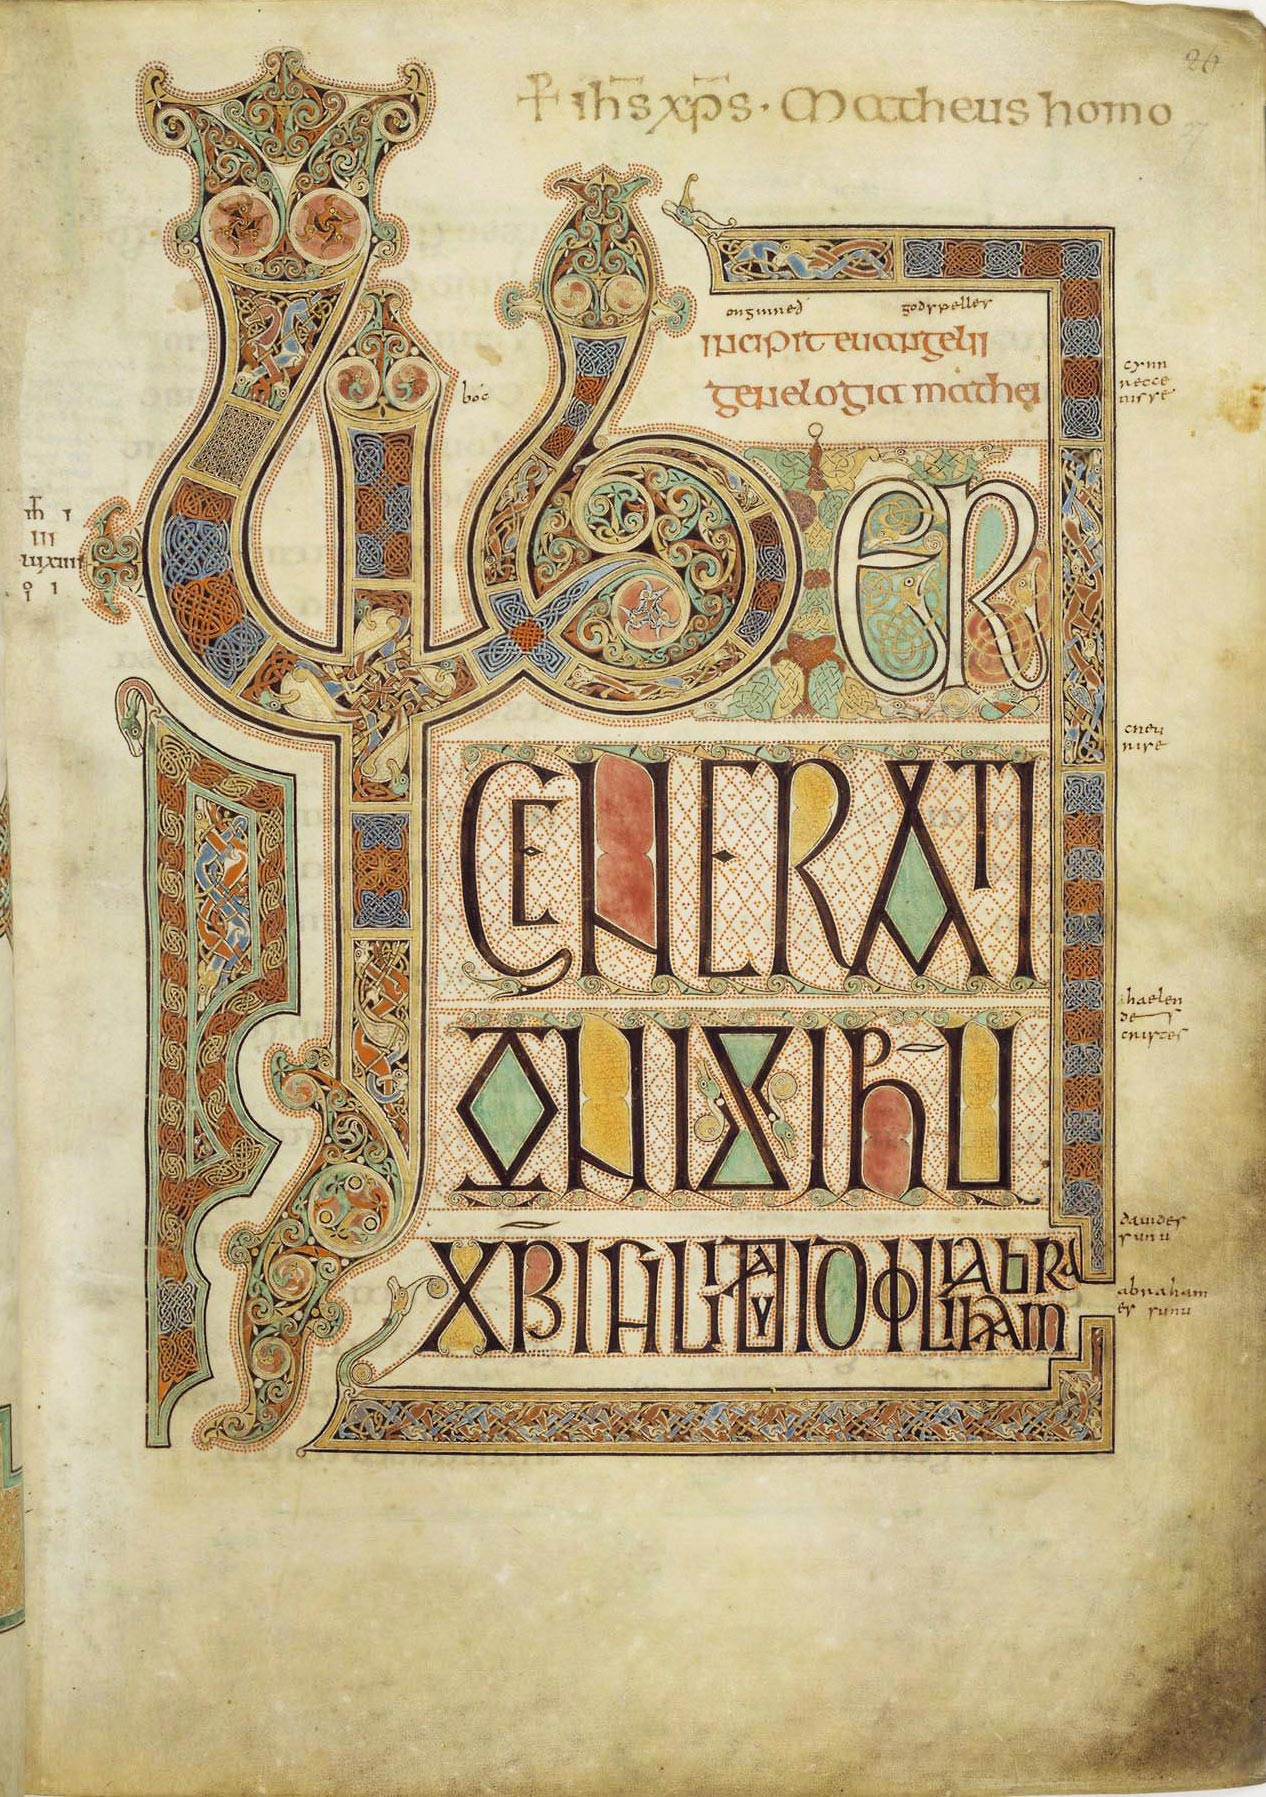
\includegraphics[scale=.09]{a20111224FearsofWhatMayBeErringPopesCouncils-img001.jpg} 
\end{wrapfigure}

\emph{Extra Ecclesiam non est salus: without (outside) the Church there is no salvation. }This was the motto of the Christian Church during the Medieval Era, and (supposedly) that which is objectionable in the Church today – the neo-pagans argue that the Church assimilated and reduced what it could not destroy.\emph{ This argument is actually true, but not in the sense which the neo-pagans intend it to be. }The Church did indeed enter a phase of development which represented a diminution, but it was not because it had combated paganism, but because it had decayed the patrimony which those same pagans had entrusted to it.


Specifically, the Church rejected the tripartite definition of man which had been handed to it by those who converted into the Church because they saw something worthy of merit which completed their aspiration. The Fourth Council of 869 AD (note that Constantine had long ago ``done his dastardly deed") repudiated a sophisticated, metaphysical view of man's nature in favor of something more exoteric and easy to understand.


\begin{quotex}
Though the old and new Testament teach that a man or woman has one rational and intellectual soul, and all the fathers and doctors of the church, who are spokesmen of God, express the same opinion, some have descended to such a depth of irreligion, through paying attention to the speculations of evil people, that they shamelessly teach as a dogma \emph{that a human being has two souls}, and keep trying to prove their heresy by irrational means using a wisdom that has been made foolishness.

Therefore this holy and universal synod is hastening to uproot this wicked theory now growing like some loathsome form of weed. Carrying in its hand the winnowing fork of truth, with the intention of consigning all the chaff to inextinguishable fire, and making clean the threshing floor of Christ, in ringing tones it declares \textbf{anathema} the inventors and perpetrators of such impiety and all those holding similar views; it also declares and promulgates that nobody at all should hold or preserve in any way the written teaching of the authors of this impiety. If however anyone presumes to act in a way contrary to this holy and great synod, let him be \textbf{anathema} and an outcast from the faith and way of life of Christians.\footnote{Source: \url{http://www.piar.hu/councils/ecum08.htm}}

\end{quotex}

The esotericism of the Church which had survived Justinian's codification was declared out of bounds. The time of this council was well after the ``Roman" phase of the Church had ended, after the chaos of the Dark Age invasions by Lombards, Franks, etc. The Roman Catholic Church (RCC) was essentially struggling to maintain what it could, both of the Greek connections \& the ancient Roman ones. John Romanides\footnote{\url{http://www.romanity.org/htm/rom.03.en.franks_romans_feudalism_and_doctrine.01.htm}} has some helpful articles detailing the unintended consequences of Charlemagne's adoption of Rome. Although he is incorrect to exaggerate the damage done from a proto-Greek perspective, he is certainly right to perceive that the chaos of the Western invasions did immense damage to all Roman institutions. \emph{Conditions in the West were so bad that Church fasts were lifted in order that populations might eat meat in order not to starve}. For the West, it was the Roman Church, or nothing – Chaos. It is unfair, then, to assume that perfect freedom of choice was exercised when the Church ``misplaced" or misunderstood its patrimony. Esoteric meaning can be lost in the best of times (just look around you); how, then, can we assume a deliberate error? Instead, one ought to look for what is best.

The case of Iceland\footnote{\url{http://www.pitt.edu/\~dash/njal100.html}} proves the point; one man's respected voice won a reprieve for paganism there, but only a private toleration – this man was actually a pagan priest. Additionally, the main proselytizing was done on the basis of ``trial by battle", a conflict in which (apparently) the archangel Michael came out over the berserkers, rune curses, and armies and storms of the pagan Gods.\emph{ And what was the price? Not to eat horsemeat, nor to expose the infants at birth to the elements!}

Note, also, that the conversion was done by royal decree \& blessed by a heathen seer who had converted :

\begin{quotex}
Shortly after Olaf Tryggvason became King of Norway he decreed that the old faith should be discarded and replaced with Christianity. His decree extended also to the islands of Shetland, Orkney, and Faroe.

When news of Norway's conversion reached Iceland, it was received by many with great anger. ``It is monstrous," they said, ``to forsake our ancient beliefs."

But Njal, a respected leader known for his ability to foresee the future, replied, ``I support the new faith. I believe that Christianity is a better religion than our old one. Those who accept it will be happy."

\end{quotex}
The rune magic which was supposedly lost was already very weak, just as Druidism had already been proscribed through battle and law by the Roman Empire. See, for instance, the account of the battle at the Isle of Anglesey\footnote{\url{http://www.philipcoppens.com/anglesey.html}}. Christianity actually preserved many remnants of paganism and gave them (arguably) a new life. This is not to minimize the bigotry of (for instance) Norman priests in England after the Conquest, but is merely to recognize that the policy of the Church towards paganism is not a simple matter of clear-cut answers. Surely, if paganism had been potent at that point, St. Boniface and others would not have been able to hew down sacred groves for firewood? When King Edwin converted based on the famous sermon with its analogy of a sparrow flying through the hall, from one door to the other, the instance\footnote{\url{http://markmeynell.wordpress.com/2010/09/10/king-edwin-of-northumberlands-conversion-and-the-sparrow-in-the-storm/}} proved that paganism had already lost the metaphysical knowledge of its own rituals.

Steiner\footnote{\url{http://www.bibliotecapleyades.net/biblianazar/ahriman04.htm}} and others offer a different account of what was occuring at the time, which has an attraction neo-paganism lacks – it is esoteric. It purports to be the revealing of the inner-ness; neo-paganism (on the other hand) seems to (often) an appeal to a neo-liberal conception of ultimate ``freedom of religion", rather than a cosmic account of history.

\begin{quotex}
Perhaps the most brilliant and influential proponent of this Arabian culture were the Caliph Haroun al Rashid and his associates, in the Eighth Century AD. This culture was, as indicated above, brilliant in a way, but was also anti-evolutionary in that it failed to appreciate the Christ-Impulse and was infected with the Sorat/Ahriman influence from Jundi Sabur. Around this time the cosmic Intelligence began to ``fall to earth", out of the rule of Michael and in the ``heads" of Men; the Pan-Intelligence becoming individualized, personal intelligence. This process was a preparation for what was to culminate after the dawn of the Consciousness Soul Epoch in the Fifteenth Century: that Men were to experience their thoughts as coming from out of themselves, as a personal intelligence in individual freedom. In 869 AD the fateful Eighth Ecumenical Council in Constantinople declared to be heretical the doctrine of ``trichotomy": that the Man is body, soul and spirit — thus effectively ``outlawing the spirit" in Western Christendom, and plunging West-European mankind ever more deeply into material experience. While this Council was happening on earth, in the soul/spirit world Haroun al Rashid and his associates, who had recently died, conferred with the individuality of Aristotle and associates: Alexander and the ``Aristotelians", together with the ``Platonists" and the Knights of Arthur's Round Table. In this meeting Aristotle and his associates resolved to bring to earth a renewed and Christianized wisdom suitable for the epoch of individualized intelligence of the Consciousness Soul, but al Rashid and his party remained opposed to this Christianization. Subsequently, on earth, the Arabian impulse was carried forward by philosophers such as Avicenna and Averroës, who upheld a decadent and retrogressive quasi-Aristotelianism, which denied human-spiritual individuality surviving death. And the Platonists descended to earthly incarnation, up through the Twelfth Century, as teachers of the Christianized Nature-wisdom of the School of Chartres. (This wisdom later inspired Bruno Latini, and consequently his pupil Dante.) In the Thirteenth Century the Aristotelians incarnated into the Dominican Order, wherein, with the help of the Platonists then in the spirit-world, they upheld the doctrine of human-individual intelligence and immortality, in the subtle conceptual thinking of the Scholastic ``Realists", as against the Arabian philosophers. The greatest of the Scholastics was Aristotle himself, incarnated as Thomas Aquinas, the proponent of the reality of Pan-Intelligence in the form of concepts — the ``universals" — and of the reality of human-individual experience of intelligence. — After the end of Medieval culture and the beginning of the Consciousness Soul Epoch, al Rashid himself incarnated as none other than Francis Bacon, the fountainhead of modern, Ahrimanic scientism. (Paradoxically, Bacon was inspired by a high Initiate, who also inspired Shakespeare, Jacob Boehme, and Jacob Balde. [Karmic Relationships, Vol. II] Again: evolution is not a simple, two-sided conflict between ``good" and ``evil" — in a way, a nominalistic-empirical science ``had to" enter cultural development.) Ahriman intends to make the now-earthly human intelligence entirely, overly individualized and personal, so that it degenerates into mere cleverness, driven by lower instincts and divorced from universal reality. But while Baconian science gained ground on earth, in the spirit/soul world the Platonists and Aristotelians convened in a ``school" under the leadership of Michael. 

\end{quotex}
No matter what one thinks of Steiner (and keep in mind Evola's definition of re-incarnation), this account is at least a ``mystery" account of the secret history of the world, rather than a Romanticization of an era which we are at least as completely detached from, collectively, as we are from the world of traditional Catholicism.  \textbf{Certainly, the prohibition of the Holy Spirit at that council would explain the submersion of the esoteric stream in the West, so that it had to re-enter the Western world via Tomberg, Solovyov, and others much later on.}

Without the restoration of the tripartite doctrine, the veredictum of history on the Church will risk becoming that of John Keat's\footnote{\url{http://www.mrbauld.com/keatsva.html}} on the clergy of his day:

\begin{quotex}
Axioms in philosophy are not axioms until they are proved upon our pulses: we read fine things but never feel them to the full until we have gone the same steps as the author. The Consecration was – not amusing — there were numbers of carriages, and his house crammed with Clergy – they sanctified the Chapel — and it being a wet day consecrated the burial ground through the vestry window. I begin to hate Parsons — they did not make me love them that day – when I saw them in their proper colours — A Parson is a Lamb in a drawing room and a lion in a Vestry. The notions of Society will not permit a Parson to give way to his temper in any shape – so he festers in himself – his features get a peculiar diabolical self sufficient iron stupid expression. He is continually acting. His mind is against every Man and every Mans mind is against him. He is an Hippocrite to the Believer and a Coward to the unbeliever – He must be either a Knave or an Ideot. And there is no Man so much to be pitied as an ideot parson. The Soldier who is cheated into an esprit du corps – by a red coat, a Band and Colours for the purpose of nothing – is not half so pitiable as the Parson who is lead absurdities – a poor necessary subaltern of the Church –

\end{quotex}
This sad state of Churchism as opposed to Christendom will come to pass, not because neo-paganism was correct in assuming the Church to be an alien usurper upon the Northern heritage, but rather, precisely because the Church failed to preserve a heritage given it by those very pagans who converted, and failed to have it restored by those pagans who picked up their mantle and immediately denounced the world their ancestors created. This is because they are dubious metaphysicians, and incline rather to a ``poetic" view of history; even the poets knew better than that:

\begin{quotex}
This is the very thing in which consists poetry; and if so it is not so fine a thing as philosophy-For the same reason that an eagle is not so fine a thing as a truth-Give me this credit-Do you not think I strive-to know myself? Give me this credit-and you will not think that on my own account I repeat Milton's lines\~{}

``How charming is divine Philosophy

Not harsh and crabbed as dull fools suppose

But musical as is Apollo's lute" 

\end{quotex}
Keats saw the errors of the Church, but used poetry to intuit the ancient doctrines of ``the vale of soul-making" \& the ``house of many mansions" — it's a pity he couldn't have read Guenon on states of being. It would be easy to pillory the Church (and I agree with Keat's analysis of many parsons), but it is the harder (and more productive) to abandon invective, and to pursue the ``great work" of following the Spirit.

Tomberg puts it this way:

\begin{quotex}
Dear Unknown Friend, do not interpret what I am saying in the sense that I am opposed or even hostile to the above-mentioned societies, fraternities, and movements of a spiritual and initiatory nature, nor in the sense that I am accusing them of an anti-Christian attitude. Do not attribute me with a lack of respect for the mahatmas and gurus of India. It is a matter here only of the purely psychological tendency (that I have been able to observe something of everywhere) which prefers the ideal of the superman to the ideal of the Son of Man. 

\end{quotex}
Tomberg goes on to add (this is the sixth chapter of MotT, the Charioteer) that the tendency is everywhere resisted in these organizations, that tendency to the three temptations of mania, inflation, and megalomania. But he insists that it is most effectively combated within the doctrine of the Church, which teaches that ``the Lord" safeguards the sanity \& humility of the initiate.

Isn't this what the West has always aspired to? The mutual recognition of truth under the umbrella of Truth? What is to prevent the practice of this, upon either side of the Roman wall?



\flrightit{Posted on 2011-12-24 by Logres }

\begin{center}* * *\end{center}

\begin{footnotesize}\begin{sffamily}



\texttt{Charlotte Cowell on 2011-12-25 at 13:27 said: }

A few thoughts sprang to mind when I read this. Firstly (in passing, really), I had never heard of this `twin soul' heresy or that it was so controversial. I think I need more info about what is what – are literally two souls what is meant or is it a soul and spirit issue?

Secondly, I agree Steiner can shed light on very difficult parts of the path, although I do not necessarily share his express view of reincarnation. Reading this made me wonder whether viewing reincarnation as a form of channelling might help solve the problem (making it more a question of terms)?

I think the Chariot card may be number 7 but either way I was put in mind of the Phaedron Charioteer and the twin horses of the soul – maybe some are getting the soul confused with its horses? Just an idea, here's an extract by the way: \url{http://alchemical-weddings.com/alchemical-weddings/the-phaedrus-charioteer}

I just found something from The Chariot card on my blog, the philosophy of a lunatic, which always amuses me:

\url{http://alchemical-weddings.com/alchemical-weddings/philosophy-of-a-lunatic}

I tarried not to tie my sandal shoe, but haste, post haste, through air my winged chariot flew (Aeschylus, Prometheus Bound)


\hfill

\texttt{logres on 2011-12-25 at 17:01 said: }

Charlotte, I've had that thought, too – perhaps there is an element (the one atom that we never replace, according to Max Heindel) which is imperishable and the seat of immortality in the soul which corresponds to Evolan individuality, but (then) the ``truth of reincarnation" would simply be the experience of having a supra-personal + sub-personal ``flame" of being passed on which records an imprint of the seat of immortality (in worship of the previous bearer). ``Channeling" could work that way. Incidentally, I need to ask you a question about waking up in dreams. I've had a lot of dreams where I am doing things with my hands, but can't remember to ask myself why.


\hfill

\texttt{Charlotte Cowell on 2011-12-25 at 17:14 said: }

well the way I see it we all have a spark of the divine with us, and the way of return is analogous to the Kabablistic process of `raising the sparks', by which all souls/spirits return to the divine source. But I can see how the idea of it being a flame lends itself to the notion of passing on the torch. In the case of a great light like St Augustine, you might reasonably expect many torches of inspiration, wisdom, etc to be lit as a result of his endeavours, although you wouldn't necessarily say he's reincarnating over and again in students. It just suddenly struck me as I was reading that part of the post about Steiner that Thomas Aquinas might well have ended up `channelling' Augustine if he studied his works in great depth and fully absorbed them into himself. What intrigues me more is how Steiner saw himself. Clearly Steiner was clairvoyant but clairvoyant vision is so rich in symbolism and has so many layers that perhaps it's all just a matter of interpretation. Certainly Steiner doesn't go out of his way to spoon feed or make things especially simple for his readers….often he's very challenging, I think he's the sort of teacher that can be wrong so the student can reach a correct answer. Mystery teaching isn't `easy' at the best of times, let alone from beyond the grave. 

What do your hands look like, what kinds of things are they doing?


\hfill

\texttt{Charlotte Cowell on 2011-12-25 at 17:17 said: }

or maybe it was Aristotle, I can't remember, point still applies tho…didn't Aristotle use ellipses?!


\hfill

\texttt{logres on 2011-12-25 at 22:26 said: }

Typing, right now! Ring on finger, left hand, wedding. I've tried to memorize the vein patterns, or note scars. Lately, have been trying to be ``aware" of them at odd intervals in the day. Realized I usually look at object ``in hand", not at them.


\hfill

\texttt{Charlotte Cowell on 2011-12-26 at 09:38 said: }

when I saw my hands in a dream I was taken aback by how they looked, it wasn't like looking at my physical body


\hfill

\texttt{logres on 2011-12-26 at 12:26 said: }

I can't remember to look, in the dream.


\hfill

\texttt{Caleb Cooper on 2011-12-26 at 16:07 said: }

You're lucky that you saw something so beautiful Charlotte. The night after you first mentioned the practice I decided to look at my hands while dreaming. They took on an unstable character, the fingers fusing together and separating, their size distorting around the edge of my awareness, in a reminder of the ugliness of my unintegrated soul. 

It was a strange experience. Like my awareness was trying to catch and hold the hands in a stable form, but it was too slow, traveling through an unpleasant invisible molasses, and right when it might catch them it hit a thicker patch a few inches from the hands which it would slide off, the hands distorting with the slipped awareness. 

Had a more pleasant experience looking at my hands in a dream tonight. I didn't see the luminous body or anything, but they appeared quite beautiful, probably because I was holding one of my soul fragments in my palms and healing it, so there would have been a very high stable frequency going through them at the time. But when I'm not elevated above my base state, yeah, pretty ugly. I should experiment with focusing the awareness on other parts of my body in the dreaming so I can see just how fucked up my soul is there as well:)


\hfill

\texttt{Boreas on 2011-12-26 at 16:36 said: }

This conversation brought to my mind a music video that reminds me about dreaming, dreams and the astral world in general – and about hands. I don't if the symbology in the video is some kind of a ``hint" to dream workers, but even if it's not, it's still quite fitting: \url{http://www.youtube.com/watch?v=0rs\_NRyNs4o}

(You need to look it through to understand my point.)

Years ago, when I tried to awake in my dreams and did practices to accomplish this, one of the basic practices was to serach for my hands in dreams and to memorize this while in awake in order it to become a habit while sleeping and seeing dreams. I never got any amazing results this way, but I think and have heard that many have.

Hands, like eyes, are the mirror of the soul and its constituting principles, and the alchemical planetary correspondences and the chakric correspondences can tell alot about many things; I always get smaller or bigger cuts and wounds in my fingers or palms if there's something that I've done or said wrong – the size of the ``reflection" (=wound) symbolising the level of the mistake, and the place of the wound the corresponding principle to look up to.


\hfill

\texttt{Boreas on 2011-12-26 at 17:19 said: }

Charlotte said: ``I think I need more info about what is what – are literally two souls what is meant or is it a soul and spirit issue?"

I don't have the exact information, but it might be a major mis-interpretation of the concepts of the animal soul and the rational soul, and the corresponding teachings in different traditions (kabbalah tree of life, germanic / nordic paganism etc.)

\texttt{Logres said: ``What is to prevent the practice of this, upon either side of the Roman wall?"}

The same as always: human stupidity and selfishness combined with myopic worldly goals. But lets not lose our hopes that at least those ``who are still gathered at the Vulture's peak" (or listening the ones who are gathered there!) understand and learn how to reconciliate their own paths and personal truths in the light of the greater unity.


\hfill

\texttt{Charlotte Cowell on 2011-12-26 at 17:29 said: }

Caleb, they did not really look beautiful more strange – translucent and kind of grey, I was quite weirded out by it, as I was when I saw my astral self in a mirror once, that freaked me out a bit


\hfill

\texttt{Charlotte Cowell on 2011-12-26 at 17:31 said: }

Boreas, the hands thing is the method taught my Don Juan to Carlos in the Carlos Castaneda novels – it is not so much the fact that one is looking at the hands that makes one conscious, but the fact one remembers to do something – looking at the feet would presumably be as efficacious, although there is something about hands as you point out….


\hfill

\texttt{Boreas on 2011-12-26 at 17:39 said: }

From the link to the article `Iceland Accepts Christianity' this caught my eye…

``In the meantime, the chieftains meeting at the Althing outlawed Hjalti Skeggjason for having blasphemed Freyja and Odin by calling them a bitch and a dog in his poem."

…and sent streams of joy through my soul, haha.

But seriously speaking, it also reminds one about the fact how easily the old truths are forgotten and denied in the frenzy of `conversion' (apparent or real), for better or for worse (usually the first option), and how easily the baby is thrown away with the bath-water.

The Gods never left the old heathens, the heathens forgot and abandoned them to a great extent, and they also failed to renew their traditions in the way that they would have provided them the needed spiritual and cultural nourishment. Now the same fact applies greatly to both neo-pagans and to (neo-)christians, while at the same time on the outer world fundamentalism, atheism and nihilism abound. This is why a synthesis in the light of universal esoteric knowledge is so greatly needed in our time and in the following age.


\hfill

\texttt{Boreas on 2011-12-26 at 17:40 said: }

Argh, a slip!

``usually the first option" –{\textgreater} usually the \_second\_ option


\hfill

\texttt{Boreas on 2011-12-26 at 18:00 said: }

OK. Based on this I take it could be an old shamanistic practice, since Castaneda fused (and confused) many teachings on his writings. I don't think it's the same – or a mere practical thing – if you look upon the hands or upon the feet. The right HAND path \& left HAND path and so on…!

However, here's one animation link for the chakric correspondences:

\url{http://www.iloveulove.com/images/ss\_kundalini\%20anim.gif}

And a picture for the planetary correspondences:

\url{http://ccrsdodona.org/images/1977\_sag\_palm1.gif}

The color scales and the planetary symbols co-incide and relate to each other quite well, yet I'd say that the either the Sol symbol in the planets or the golden color upon the chakric finger correspondences are mis-placed.

``The science of hand-reading, strange as this may seem to those who have no notion of such things, is, in its Islamic form, directly related to the science of the divine names: the arrangement of the principal lines of the left hand trace out the number 81, and those of the right 18, giving a total of 99, which is the number of the names attributed to Allah (sifatiyyah). As for the name Allah itself, it is formed by the fingers in the following way: the little finger corresponds to the alif, the ring finger to the first lam, the middle and index fingers to the second lam, which is double, and the thumb to the ha (as regularly drawn in its `open' form): and here lies the principal reason for the widespread use of the hand as a symbol in all Islamic countries. From this we may understand the meaning of the verse in the book of Job: `He seals up the hand of every man, that all men may know his work': and it may be added that this is not unrelated to the essential role of the hand in the rites of benediction and consecration…"

– René Guénon, Insights into Islamic Esoterism and Taoism'


\hfill

\texttt{logres on 2011-12-27 at 00:54 said: }

Thinking about this today (I appreciate all the helpful comments, maybe this will help me) – the hands are the active part of the soul. When the mind is SURE and stable, you can concentrate on doing with the hands. Perhaps, in a dream, the hands can only become visible when the mind has reached a certain stability. Also, you may be reaching to DO something in a place that you are not yet ready to act – hence, the wavy hands. Heindel teaches that in past epochs, as the vehicle of the body was prepared, the spirits were attached, but not fully incarnated – they then experienced through the body, but not fully as we do. Something similar is going on with the hands in dreams. A fully awake person would have dream hands that were beautiful. Or at least not streaming off somewhere. They may be connected to another place, even inside the dream. That is backward, from the hands, down, rather than from the feet, up.


\hfill

\texttt{Charlotte Cowell on 2011-12-27 at 08:08 said: }

well the real and/or imaginary Don Juan was eminently practical, and when he revealed the purpose of the exercise to Carlos he said that it was the consistent effort involved with trying to see the hands (or whatever) that made the unconscious self absorb the practice so completely that at some stage one will inevitably see the hands. It's interesting what the Sufis/Guenon said about hands and one intuitively feels there's something significant about this part of the body having been chosen, but in the `Don Juan school' they're not relevant in this way. His goal was simply to heighten perception. I've never heard of the hands streaming off or away before, or any other part of the body, that sounds like a dream to me. As far as I'm aware the astral self doesn't dissemble in this way and (in my experience) people generally appear as their most beautiful possible selves in that state, it can be quite intersting to see how the otherwise secret character and beauty of an individual manifests, especially with respect to the light in their eyes.


\hfill

\texttt{logres on 2011-12-27 at 13:48 said: }

It was just a speculation – I've heard the hands look wispy or wavy, suggesting a movement to another plane. As I say, I've yet to accomplish it – my dreams for now are rather jumbled, although changing. Happy twelve days, to all!


\hfill

\texttt{Caleb Cooper on 2012-01-01 at 16:51 said: }

On the original post, I think Rome's position is a little more nuanced, and if I understand correctly, compatible with Traditional teachings on the tripartite nature. 

At my last RCIA class before Christmas break, there was a reading from St. Paul in which he used Spirit distinct from soul, giving me the opening to ask the Deacon what the Catholic distinction between them was. The Deacon's explanation was that God has breathed a Spirit into all men, and this Spirit is the Holy Spirit. I was quite pleased to hear this, as it seems essentially in agreement with Tradition, that the Spirit in man is a fragment of God, which also contains the entirety of God (like a hologram).

I'm not familiar enough with Church history to speak with authority, but what Constantinople IV may have been objecting to was the demoting of Spirit in man to the level of a soul, in which case they were actually defending the tripartite view of body/soul/spirit against body/lower soul/higher soul, which cuts man off from the higher spiritual vistas.


\hfill

\texttt{logres on 2012-01-02 at 01:00 said: }

Caleb, that's actually a very astute comment, \& Cologero privately pointed out the same thing, so the Council's ``error" may have been more one of context (ie., in the process, losing the instinctual point and definite dogma being incidentally touched upon by way of clarification) than of intent. A study on the dearth of tripartism in the Church might prove interesting and turn up more facts. This was meant to be introductory, \& I obviously have a lot more to learn on the subject. However, the lack of clarification or context is troubling.


\hfill

\texttt{logres on 2012-01-02 at 01:08 said: }

Boreas, the blaspheming poet got what he deserved, so it's comforting that there is some justice in the world. You may be interested in \url{http://www.sacredscience.com/archive/GodwinArcheometer.htm}, although you sound like you've already been over this ground.


\hfill

\texttt{Dimitri on 2023-03-08 at 12:51 said: }

Actually, I'd like to issue a correction to this article. I did some digging on the point of the Fourth Council of Constantinople (the Catholic one) because I found the language of Canon 11 suspicious, in that it didn't seem to be condemning a tripartite view of man; after all, why would it condemn the idea that man has ``two souls" (which is not the tripartite view), rather than both a soul (anima) and a spirit (spiritus), if they have two separate words for both in Latin? As it turns out, it was doing no such thing:

``The eleventh canon anathematizes the doctrine that a human being has two souls. This refers to a doctrine promoted by Photius, that each man has two souls, one that is liable to error and another that is immune to error. Photius himself did not believe this doctrine, but gave arguments in its favor in order to prove that theologians could not afford to ignore philosophy. Many people took these arguments in earnest and believed the doctrine, requiring its repudiation here." (Commentary on the Fourth Council of Constantinople, \url{https://www.arcaneknowledge.org/catholic/councils/comment08.htm})

Upon digging into the matter further, I found corroboration for this when I looked into what Photios the Great was attempting to do by putting forth this teaching:

``In a feud with Patriarch Ignatios, Photios invented a fanciful theory that people have two souls, for the sole purpose of tricking Ignatios into embarrassing himself by being seen to take it seriously, whereupon Photius withdrew his proposal and admitted he had not been serious."

Historical context is important, folks!


\hfill


\end{sffamily}\end{footnotesize}

\section{Harmonics}

In order to win the daily battle\footnote{\url{https://gornahoor.net/?p=3005}}, we may resort to any number of tactics which can strengthen the ``core" of man by magnetizing the higher centers of his personality, including plain music\footnote{\url{http://www.youtube.com/watch?v=IoSuyUFiEYo}}. As several correspondents on this site have suggested, there may be a harmonic basis for this in Solfeggio notes\footnote{\url{http://www.youtube.com/watch?v=9su8OVjewS0&feature=related}}. Counterpoint, basso profundo, \& harmonics may provide us with a means of understanding the polyphony (and seeming polytheism) of Life. Music teaches us to eschew the demon of dialectics, as well as helping to cure the demon of the noonday sun\footnote{\url{http://www.johnsanidopoulos.com/2012/01/their-noonday-demons-and-ours.html}}. We can use it to see harmony, rather than conflict, or conflict-in-harmony.

The ``diamond self" (it is averred) is the opposite path from the dissolution of the self and resolution of the new Self in Christ; even Tomberg emphasizes this in his \emph{Meditations}, that the path of the East is to withdraw into the self, and it is valid, but not highest. After all, there are many stars in the night sky, all of them real, no doubt many glorious, but there is but one North Star which we may steer by in our humanity. And this, in fact, is true. The Medieval Era, whatever else it is, is the paramount Age of Man, Man as Man. Just as ancient times were the times of the gods, and modern times are the times of the robot and the beast, the Middle Ages were the time of Man.  Likewise, Christianity is (or should be) the religion best calculated to preserve that which makes us human, as a trophy and shield to bear into heaven.

\begin{wrapfigure}{rt}{.3\textwidth}
 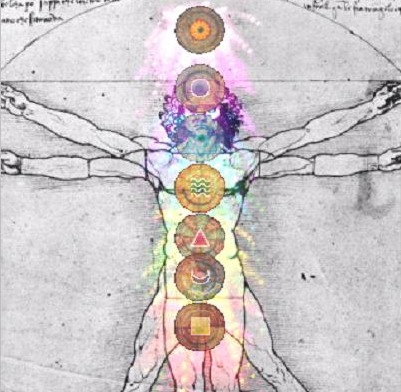
\includegraphics[scale=.5]{a20120107Harmonics-img001.jpg} 
\end{wrapfigure}

However, what if ultimately (in the post-mortem states) these two paths, the path of the Diamond, and the path of the Hermit, are not (in fact, finally) separated? We already intuit this to be so, since Christianity claims that Christ's final act will be the conquest of Death and Hell, the Recapitulation of all things within the Logos, where, at the end of Time, he will surrender his \emph{imperium} back to the Father (see Colossians). Will the Logos, through whom all things were created, lose something given to His care? Thus, the survival of one avatar of Man upon the path of the Hermit means that those of the Diamond Self, the wandering stars, will be at the end of time, gathered back into the fold. It is possible to be a Super-Man, your own Christ, because of the final Christ, found not during your stay in the vale-of-soul-making\footnote{\url{http://academic.brooklyn.cuny.edu/english/melani/cs6/keatsltr.html}}, but later, in the houses-of-many-mansions, at the end of time.

We see this to be so from the breath. Man breathes in, then exhales. With close attention, one can tell that it is the ``breathing out" (or surrender) which collapses the chest and pulls the life down into the spiritual heart, whereas the breathing in raises the spirit in exaltation. But then again, in effect, the breathing in is also (in its way) a prayer to above, although it is more aggressive in taking. Likewise, one can see that breathing out might be taken as a rejection of God, or a letting go of even Him. The breath, although in two paths, is finally One. There is one breather, one breath.

The path of the diamond self is simply the continuation of existence (or a certain form of it) in the post-mortem state, indefinitely, which will trace its own way back to God. The path of hermit is actually swifter, though it seems to tarry in the fields and byways and inns of the ring of the world. One ``makes haste, slowly".

Which is better? Which is more noble? Since they are finally the same, the choice is left up to us: ``Whatever you bind on earth, will be bound in heaven; whatever you loose on earth, loosed in heaven…be careful how you judge – which ever way a man judges, in that way shall he also be judged…" Does the Super-man wish to be without the Self of higher Selves? How can he be God, if there is no God? What else does it mean, to say, the Lord has given him a name above every names, highly exalted? There are many little Christs; if there were not, how could we picture the Exalted One?

The chakras correspond to the sacred Solfeggio notes (the glands of the endocrine system are externalizations of the inner pathways, coagulations of serpentine energy which imitates the sacred network), and this forms the Kundalini energy trail. Here is Evola:

\begin{quotex}
Lightning moves downwards, which Evola explains it is a sort of ``command of those who have reached this supreme plane is like a thunderbolt that travels along the entire hierarchy, starting from the top until it reaches the vibrations at the very bottom, which shape matter. This is the so-called vajra-vak, the diamond-thunderbolt of the living word." (TYoP, page 13) The cyclical nature then allows the initiate to `shape matter'. Then he begins again at the bottom, as Evola describes the process of upward moving chakras: ``Through the earth chakra one acquires an extraordinary material strength. Through the water chakra one may acquire youthful energies, thus neutralizing the processes of aging and of organic decay (``The Water of Life"). Through the fire chakra one acquires the power of transforming and of dissolving the elements (this corresponds to the Hermetic saying \textit{solve et coagula})." (TyoP, page 184)

\flright{Source: \url{http://www.joanlansberry.com/wr-hekau/serp2of2.pdf}}

\end{quotex}
Those who wish to return from the pharoah's tomb bearing a forked stick with a brazier of fire on their head will have to ``wake up", which is to initiate their chakras. But how? Do we do this alone, or with others? With the Other? As a diamond-thunderbolt who utters the \emph{vajra-vak}, or as someone supplicating ``the Lord"?

Here is Tomberg's description\footnote{\url{http://www.eleggua.com/Objects/Tomberg-Spiritual_Basis.html}} of what happens in the Christian path, which many regard as ``Semitic":

\begin{quotationx}
The power which makes man into an upright, vertically oriented being entered into men following the Fall. In essence it was what today we usually call ``pride". The Bible shows the nature of this power by the words of the Tempter : ``Ye shall be as Gods." When pride entered into human nature through the Luciferic impulse, a vertical scream, from below upwards, came into being in the human organization. The physically perceptible expression of this scream is the backbone. What has formed itself physically into backbone consists astrally of \emph{pretensions of pride.} These pretensions have themselves as object : they feed on themselves. So arises the upward streaming swirling movement of the passion of pride. The form of the vertebral column is its physical expression.

Now the basic pre-condition for the Manas revelation is that a stream must come into being which goes in the opposite direction : from above downward. Regarded \emph{spiritually ,} it is the stream of revelation ; as soul-phenomenon, however, it is borne on the stream of \emph{humility.} But opposing it is the pride which lives in all human nature since the Fall.

Therefore, in order to make it possible, a purification of human nature must precede the Manas revelation. This purification consists in the dying out of pride in that part of the astral body required for cognition. Man has to submit to a process of \emph{humiliation} which brings the Manas organization to maturity. This humbling is accomplished as follows : The man who out of the forces of his consciousness soul has chosen the spirit will be, as it were, `incarcerated'. On the one hand, a protective wall will be erected around him against evil influences ; on the other hand, a dome arches over his head consisting of the \emph{silence of the spiritual world.} Thus arises an \emph{empty} space where the man is quite alone. This space is so empty that even evil cannot enter there. The man has an opportunity fully to experience his powerlessness and poverty. He also grows fully conscious of the nature of his personal feeling of pride in all its vanity, and the powerlessness of his pretensions. In this emptiness of soul and silence of the spirit, his pride gradually dies away — until one day the decisive hour arrives in which the man feels himself to be a broken hollow reed and finds no more strength in himself to stand upright in the world. For what has held him upright since time immemorial, the power of his pride, is now broken ; the core of life for his personality is wiped out. Then man experiences himself as \emph{so} empty that there remains only one thing to do : to give the last breath of his life of soul co love. When he does this, the walls of his prison vanish and heaven opens above him ; the Manas organization has matured. The ``vertebral column",which through the death of pride had become a hollow reed, is filled \emph{from above} with the love-revelation of the spiritual world. So he becomes again an upright being — but in quite another sense than before. He now stands upright because he knows himself to be a connecting link standing between heaven and earth. For the \emph{new} wisdom of world evolution is not heaven's wisdom alone, neither is it earthly wisdom alone ; it is their harmony sounded on the strings of the human being who is stretched between heaven and earth.

A similar ``imprisonment" of the human soul also takes place after death. \emph{Kamaloka} is not a world, but a \emph{condition of the} human soul. It is a condition in which the soul is closed off from all that happens in the world. There it goes through the purification brought on by its state of being alone. ``Imprisonment" takes place not only on the path of cognition and after death, but sometimes in the course of destiny of human individuals on earth. So one will never understand the deeper destiny-tasks of such individualities in the history of mankind as, for instance, Mary Stuart or the Man in the Iron Mask, if one regards their fate merely as ``punishment" for the past and not also as ``preparation" for the future. The ``political" reason for imprisonment may have been the rivalry between Mary Stuart and Elizabeth, it may have lain in the birth rights of the one known as the Man in the Iron Mask who was kept in prison for over forty years — but those are not spiritual reasons. The spiritual reason these personalities had to experience and suffer the fate of undeserved prison loneliness is the preparation of a Manas organization.

\end{quotationx}
Now, denatured from the Semitic sense of Sin, we are still describing here a ``sin" which exists as the ``vertical scream" upward of serpentine power attempting to seize what it has not earned. It is worth nothing that this criticism can be made from ``Aryan" principles – honor to whom honor, etc., rather than ``sin". Is not God, if a person, due certain honor? Was this not the basis for the medieval conversion of the tribal kings to the Lord of Glory? Although Jesus spoke of taking heaven by storm \& violence, what is done here is (according to Tomberg) actually against the organization of the spinal column itself. The spine is not ``an eternal circle", but rather a rising spiral – that is, the serpent's power of cunning has  been broken into by vertical energy. Thus, the spinal column makes an eternal circle going up \& down, a Jacob's ladder. Additionally, due to the vertical ``raising" of this column to the solar power of the Sun (and here is the Hyperborean religion), continual influx of vertical power can reach the spinal column and enter into the human being. In this manner, the serpent is hoisted aloft upon the brassy pole, and sacrificed for the sake of those who live ``under the Sun", that we might become eternal stars of righteousness, though some differ in glory, as one star the other. Man walks – that is, he is man, suspended (as on the Tarot card) or hung between heaven and earth, upside down. The Middle Ages were the supreme time period for the recognition of all that it meant to be man.

This is why Jesus proclaimed his ``yoke to be easy, his burden light". Not because it was, but because it offered a means of saving the poor sheep of personality (the human element) which other paths of breaking out of the eternal circle did not, at least until the final in-gathering. Additionally, it was the fountain, capstone, polar star of all the methods, in that (once the post mortem states are reckoned at the end of time), ``He will be all in all". The scattered, diamond-thunderbolt wandering stars of others who have gone their own way will return, or be gathered in.

\emph{Tomberg has much more to say about the solarization of the intellect, the selenization of the will, and lunarization of the imagination, as well as the chakras, which sheds light on the Hyperborean relationship to Christianity. }



\flrightit{Posted on 2012-01-07 by Logres }

\begin{center}* * *\end{center}

\begin{footnotesize}\begin{sffamily}



\texttt{thelight on 2012-01-07 at 12:42 said: }

``The Middle Ages were the supreme time period for the recognition of all that it meant to be man." 

Can't agree with this statement (since it ignores lost knowledge) but it is valid to the point that we can only work with what has been handed down to us, if we take what remains of our derelict organized faith (Catholicism). The middle ages only held partial revelation. 

Do you actually believe that there is a continuum of consciousness in the ``post-mortem states" (i.e, an after-life in the genuine sense of the term) or is this more poetic-metaphor cad?


\hfill

\texttt{Logres on 2012-01-07 at 18:49 said: }

Tomberg thinks that there is a purgatory, either of the serpent, or of a progress to God, the Church teaches it, and the ancients believed it, so that's good enough for me. Additionally, I have had a supernatural experience which confirmed a post-mortem state, or at least a preternatural one, for some entity, an experience not sought for by myself, so yes, we don't ``die" except insofar as our physical body is concerned. What happens to those who don't go to God is the subject of several chapters in Tomberg's book – re-incarnation (Gurdjieff's teachings) are based on the electricity of the irritation between Yes/No in man. Poetry can be a swamp, but it can also be disciplined into ``seeing". 


\hfill

\texttt{Matt on 2012-01-08 at 04:15 said: }

Logres,

Would you agree that the initiated continue their existence after the dissolution of the physical body, but the uninitiated cease to exist, or maybe more accurately exist at a mere unconscious/larval level, when their physical bodies die?

And another good entry.


\hfill

\texttt{thelight on 2012-01-08 at 08:50 said: }

Does Cologero stand by the belief in a ``post-morten state" of consciousness? I'm unsure if Evola stood by that claim, rather it was seeing things in a metaphorical sense, but since actions done while alive has cause and effect, they are ``immortal". Also understood is the idea of ``flame to flame" and your presence living on in others etc (not to leave out the phenomena of psychic residues and larval states such as ``ghosts"). All of these happenings are materialistic views and do not suggest a conscious being continuing life after death of the body.

Visit here for an opinion piece on Tombergs' Meditations on the Tarot : \url{http://billcork.wordpress.com/2007/03/29/tombergs-heretical-nonsense/}.

Logres, it's also hard to say for certain if OBE's are not projected imagery of the psyche. We would all love to believe there was a conscious survival after death of the body even through an initiatic operative method but what have we got to believe or prove this other than Faith?


\hfill

\texttt{Boreas on 2012-01-08 at 09:30 said: }

``We would all love to believe there was a conscious survival after death of the body even through an initiatic operative method but what have we got to believe or prove this other than Faith?"

In theoretical level, esoteric knowledge of the elements – both great and small, material and psychic, microcosmic and macrocosmic – based upon the universal law of correspondences.

Earth (body) dissolves to Water

Water (emotions) evaporates to Fire

Fire (intentions) disappears into the Air

Air (reason) transforms into Aether

Aether (intellect) flies into the Void

The support of consciousness in this dissolving process naturally depends upon the level of spiritual progress – or of the level of ``Manas organisation", as it is called by logres in this article. I think it can be said with somewhat certainty that some small part of consciousness goes through the transmigration process through all these phases even in the case of non-initiates, though the ``trauma of death" can blurry even this, not to mention other distracting and obscuring factors.


\hfill

\texttt{Boreas on 2012-01-08 at 09:36 said: }

``Everyone is proud of something. We are proud of God!"

– An esoteric Sufi proverb


\hfill

\texttt{thelight on 2012-01-08 at 10:04 said: }

``The support of consciousness in this dissolving process naturally depends upon the level of spiritual progress – or of the level of ``Manas organisation", as it is called by logres in this article. I think it can be said with somewhat certainty that some small part of consciousness goes through the transmigration process through all these phases even in the case of non-initiates, though the ``trauma of death" can blurry even this, not to mention other distracting and obscuring factors."

I won't hold my breath.


\hfill

\texttt{logres on 2012-01-08 at 10:10 said: }

In a certain sense, I suppose it's true that no one knows what happens after death, because we aren't there yet. While I think Tomberg would agree with what you wrote, Matt, he would caution that this belief does not become the Gurdjieff quest for creating the four subtle bodies, crystallizing essences out of each body and building them into a tower of Babel. He believes it is possible, but thinks that this is what the serpent promised Adam \& Eve (he did not lie, but offered a horizontal magic whereby mages could create a ghost body, then a body of a ghost body with intellect, then one with will and soul, etc.). They could then re-incarnate. Much of what is called ``initiation" is (in fact) this kind of lower magic, which reaches an impasse due to its specialization. This is why Scripture calls them wandering stars, and there is no hope for them until the end of time. Or, rather, they are their own hope. This is how he argues.

With regard to post-mortem states, the soul is created by God as his ``image", which is NOT defaced. The likeness is defaced, not the image. Therefore, though hell can scorch it, it cannot be destroyed. Nothing can destroy it. Scripture talks about the ``works" of man being burned up, nevertheless, the man himself shall be saved. This is what is being spoken of.

If you don't like the Bible, consider natural Reason. Is it reasonable to believe that immortality is merely a metaphor? That all intuitions, premonitions, whispers, etc. which take place in the magical current of the world are simply so much sound \& fury? Too much emphasis is being placed on the difference of the afterlife from now; this is only partially true. There is a change in the mode of existence.


\hfill

\texttt{Charlotte Cowell on 2012-01-08 at 10:41 said: }

fascinating post Logres and a lot that could be commented on! Fiery spear springs to mind….Cx


\hfill

\texttt{Charlotte Cowell on 2012-01-08 at 10:51 said: }

@thelight I think it's reasonable to say that certain types of spiritual experience are wholly or in part to do with the psyche, but OBEs aren't like that – you can easily verify they are `real' by checking in on facts, time/space are traversed differently but this world is as it is – in theory you could go visit someone, watch TV with them then tell them in person the next day what happened. i've not done this kind of thing before and I think a lot of people abuse their astral gifts by spying on others in the lower astral, but I know it is possible. A really good book to read on this subject is George Ritchie, Return from Tomorrow. It is a heartwarming, wonderful story whatever your views on this subject – \url{http://www.near-death.com/ritchie.html}. As a war veteran and psychologist he also has a lot of credibility


\hfill

\texttt{Boreas on 2012-01-08 at 15:18 said: }

``I won't hold my breath."

That's good. You really should let it go when the time comes.


\hfill

\texttt{Matt on 2012-01-08 at 15:32 said: }

Lorges,

Thanks for replying. I don't really have any disagreements with what you have written in your reply (I think we're on the same ground here). I'm also not implying that immortality is just a metaphor (though you might have been addressing TheLight there). Just contemplating out loud so-to-speak about the idea of there being a difference between the paths of the initiate (and probably not in the sense you wrote of today's typical initiate) and the common individual. Similar to what Mourieveff wrote in his book, or what Raphael Johnson has written (and spoke of in his podcast on Augustine).

I'm sure this comes across as mere rambling on my part. Apologies.


\hfill

\texttt{logres on 2012-01-08 at 19:11 said: }

Matt, I was responding to TheLight there, not you, I understood your meaning. Just wanted to be clear because I was confused on the point until I read MotT; there IS a clear distinction between ``initiate" or not, most certainly. However, the Church's teaching (which I accept) is that everyone has a spark of divinity which even their freedom is not allowed to efface. Presumably, this hologram (or whatever you wish to call it) allows God the power to ultimately redeem them (if and how and when He chooses). I wasn't aware F. Johnson discussed this. Can you link?

RE: Charlotte's point – the reason God witholds superpowers until a certain level of sanctity is reached (excepting the case of the super-men who use the serpentine energy to ape miracles or in some cases, specialize at the cost of soul and surpass them) is because the same power that can heal can presumably wound or kill. God therefore waits until a certain disposition of the will is ``fixed" in virtue – then He confers abilities commensurate with virtue. This is how the angelic hierarchy functions as well.


\hfill

\texttt{Matt on 2012-01-08 at 20:00 said: }

Here's the link Logres,

\url{http://reasonradionetwork.com/20110721/the-orthodox-nationalist-saint-augustine-of-hippo}

Maybe its F. Johnson putting his own interpretation into things, but according to him, Augustine, like a number of the church fathers, makes a difference between what the baptized and the unbaptized can expect for their future when the physical body dissolves (I guess on here we can substitute baptized and unbaptized for initiated and uninitiated).The baptized will be given immortality (whether they will experience eternity in hell or heaven is up to each individual) whereas the unbaptized will essentially return to the earth (hence not achieve immortality). I just think its interesting how it connects back to here with Gornahoor on Evola, as he makes this point too about immortality being conditional, and a mere larval survival after the death of the body isn't the same thing. This has all constantly been on my mind lately, so I just wanted to see how you've come to understand all this.


\hfill

\texttt{logres on 2012-01-08 at 22:59 said: }

You will be helped (as I was/am) by reading Tomberg – he deals as subtly and religiously with this as anyone I am aware of. There is no doubt baptism incurs a karmic debt (if the person ignores it). Keep meditating on it. If Augustine really thought that, it proves he viewed baptism as ``magic", divine, but magic. I am not sure what to think about reincarnation, ``larva", etc. Am inclined to think people lose pieces of their soul which are restored to them when someone else ``breathes them in" (this is a method of dispelling ghosts and incurring the gratitude of the spirit of the ghost, btw). This someone else then can keep and share (return) at the same time, thus becoming a karmic ``servant" who is ``exalted". Jesus (then) would have done this on a grand scale. But how small can one make a soul before it disappears?


\hfill

\texttt{Cologero on 2012-01-08 at 23:27 said: }

No, Mr. Light, we do not stand by any belief but rather stand on gnosis. If you prefer authorities rather than your own self-awareness, you can read our posts on the Ancient City and the veneration of ancestors. In the Bhagavad Gita, we read:

\begin{quotex}
When adharma (impiety, unrighteousness) overwhelms the family, O Krishna, the women of the family become corrupt; and when, O Krishna, the women are corrupt, there arises a mixing of castes. This mixture leads into hell the family itself as well as those who destroy it; for their ancestors fall, deprived of the offerings of rice-balls and water. \flright{\textsc{Ch 1:41-42}}

\end{quotex}
Swami Nikhilananda offers this interpretation:

\begin{quotex}
The reference is to the Hindu religious rites for the dead, known as the sraddha ceremony, in which rice-balls and water are offered by the eldest son for the satisfaction of the soul of the deceased. This ceremony cannot be performed by children born of irregular marriages … Deprived of the rice-balls and water, the soul of the deceased, according to Hindu tradition, goes to hell. The offerings of rice-balls and water is a symbol of loving and reverent thoughts for the dead, which help to foster a feeling of close relationship between the living and their forebears. 

\end{quotex}
This is the Tradition of the Indo-European peoples, although nowadays we offer flowers in the West. Note how this teaching differs from many self-defined pseudo-Traditionalists, who either refuse to beget sons, or maintain irreverent and hateful thoughts about their ancestors of the past 1500 years, or, worse, deny their continued existence and influence.

For Guenon's explication, please refer to Man and his Becoming according to the Vedanta.

Evola writes of two paths:

\begin{quotex}
This type corresponds spiritually to the ``forefather's path"—pitr-yana—which the Indian traditions speak about, also called the earth path or mother's path, according to which the individuals are dissolved entirely after death into the original stocks, in the forces of the race and forefather's blood, with which true existence alone rests. But, opposed to this path, there is the solar path or path of the gods—deva-yana—also called the Nordic path (while the first path, the path of the totem, is called the path of the South); a path which we can also call Olympic, travelled by those who make themselves immortal, who become gods, who ``go out in order not to return". 

\end{quotex}
As for the fellow perturbed by Tomberg, it demonstrates why such teachings were always passed on in secret. In our disordered age, some concessions need to be made. Of course, salvation is possible without any Hermetic teachings. But some men seek after liberation, so they have a different need.


\hfill

\texttt{Matt on 2012-01-08 at 23:58 said: }

Logres,

Yeah, I started reading Tomberg at the end of 2010. I haven't yet finished his work due to being busy with school, family, my other readings etc. But I am making it my goal to finish reading it.


\hfill

\texttt{logres on 2012-01-09 at 08:55 said: }

Matt, I'm slowly working my way through, also. Am not trying to be mystical, or put off your question, which is a good one. Cologero's answer above contains the germ of an answer to that question (baptism being birth or ancestry from above) or you can approach it theologically. One has to keep in mind that a ``personal" answer may be valid gnostically, but not valid publicly, which is where I am at – in terms of personal experience and knowledge towards me, baptism is a rite which confers a divine blessing or birth, depending on the giver and the recipient. What I would say publicly is that it establishes some kind of a link to the destiny of the Church. I wish I could go further at this point, but cannot. It is a very pressing question, which you are right to ask.


\hfill

Thanks for the vinegar sponge so far, but still I thirst. When one thinks of it, the state of post-mortem is of utmost importance. Of course it best to ``know rather than to believe", but as Often our musings, idleness and forum chit-chatter are distractions to doing the actual work that will save us (so to speak) from a rebirth to a samsaric repetition or dissolution into Hades. Perhaps it is necessary that one's being should be centered to death at all moments, and indeed how one approaches death is central to all religions and spiritualities. 

Cologero wrote : ``This is the Tradition of the Indo-European peoples, although nowadays we offer flowers in the West. Note how this teaching differs from many self-defined pseudo-Traditionalists, who either refuse to beget sons, or maintain irreverent and hateful thoughts about their ancestors of the past 1500 years, or, worse, deny their continued existence and influence."

Two things I must take issue with here. While it is loyal and honorable to revere ones ancestors, few can trace their ancestry back beyond a thousand years, let alone 30,000 yrs since the dawn of Europe (never-mind if they worshiped under a ``Semitic" god or not and if the I.E. invasions only occurred 3,000-4,000 yrs ago). Are flowers still enough food for the remembrance rites? 

On the other hand, what of celibate priests and other holy men who do not beget sons? Are these too, ``hateful pseudo-Traditionalists"? What do you make of Evolas situation then whom saw the family (biblical ``family values") as a giving in as opposed to the comradeship of a holy männerbund? There is also the Heremetic question of ``the mysterious race of perfect men, unknown to previous generations." The Royal Art of the ``Sons of Hermes"? 

Cologero: ``a path which we can also call Olympic, travelled by those who make themselves immortal, who become gods, who ``go out in order not to return"." 

Bravo. Now this quote on the Nordic path is perhaps the most significant statement made thus far but how is this literally achieved if I must ask a direct and predictable question?


\hfill

\texttt{logres on 2012-01-09 at 23:19 said: }

Well, you can always start with the hundred or so articles Cologero has put up on the site (along with others, in the past). I'd recommend the essays on the Three Trials. \url{http://www.gornahoor.net/?p=1902}

There are plenty of others, meant to direct one's inquiry, rather than to give a pat answer. I don't know your background, so you may already know this – part of the efficacy of Hermetic work consists in the student's own desire and thirst. So it depends what you are asking – if Evola is the angle you are interested in, I am sure someone on this site can help to pinpoint some texts that will assist you.


\hfill

\texttt{logres on 2012-01-09 at 23:20 said: }

Charlotte, as always, you leave me curious – what is a flaming spear?


\hfill

\texttt{Boreas on 2012-01-10 at 05:07 said: }

TheLight said: ``Now this quote on the Nordic path is perhaps the most significant statement made thus far but how is this literally achieved if I must ask a direct and predictable question?"

A good article on the subject by Guénon can be found from here:

\url{http://www.lodgeroomus.net/downloadcenter/uploads/The\_solstitial\_doors1.pdf}

Initiation and Spiritual Realization certainly has some worthy texts also about the subject of ascending and descending realizations and corresponding goals etc. If it's Evola you are interested, then I'd suggest starting with `The Doctrine of Awakening' about the subject of liberation from the cosmos.

You are certainly right that one minute of practice (meditation etc.) is worth ten hours of theory, but if the theoretical background is missing or unclear, then practice is also easily mis-directed.


\hfill

\texttt{Charlotte Cowell on 2012-01-12 at 13:30 said: }

Boreas I can't say all of what was in my head at that moment, but I can confirm that it relates to the spear used to pierce the side of Christ on the Cross. Funnily enough yesterday while I was thinking of what to say about this I randomly opened the first book in my library that came to hand and it turned out to be a passage about precisely this object. As such I found it worth detailing on my blog:

\url{http://alchemical-weddings.com/alchemical-weddings/mystery-of-the-spear}

The mystery of the spear wound points us towards spiritualisation of the physical body. The special, pure elixir that flows from the side of the Lord is certainly an esoteric reference to an esoteric process of development that occurred – for the first time, yet symptomatically for all human beings – here on earth within the space of a few hours.

(We need to counter the idea that spiritual processes and the higher developments they bring about unfold exclusively beyond the threshold, and never impinge on the sensory world. It is an erroneous gnostic mode of thought that regards the Christ sacrifice, His transformation and resurrection, as a process solely of spirit and soul. This would be a denial of Paul's teaching.

What use is spiritual development if it has no reforming effect on the lower bodies? And these lower bodies – particularly the lowest, the physical body – belong to the earthly world and can only be worked upon during incarnation. All development in the spirit aims to enliven the mortal human being.

All higher spiritual development at the same time works and impinges on matter. Serious spiritual work always leads to deed and action in the physical world. The appearance of a divine being in the material world embodied this to the very highest degree).

The spear-wound mystery is one of transformation, of etherisation; and it takes place before the eyes of those present at the time. One of these witnesses became a source of truth for us, leaving his testimony in the form of the Gospel of St John.

If this Gospel by the disciple whom the Lord loved is read in the right way it reveals to us deep truths about the Mystery of Golgotha.

Judith von Halle, Secrets of the Stations of the Cross and the Grail Blood


\hfill

\texttt{Boreas on 2012-01-12 at 18:20 said: }

Charlotte, you are absolutely correct that all real spiritual experiences are truly Earth-shattering (!); especially if there is still something rigid in our being, the effect of the spirit shatters it like focused Solar Rays crack and melt the ice. The gift of Tears!

After all, a truly Human soul is a fully lighted house with five windows of blood and living water, shining with blazing letters of light in the dark cave of the personality.

``A man of wisdom sees the world through his own windows." – Lao-tzu

Can't help linking this: \url{http://www.youtube.com/watch?v=RDS2PWRuB7M}


\hfill

\texttt{Charlotte Cowell on 2012-01-12 at 18:38 said: }

Yes I often think about the gift of tears, it's one (of many) things from MoTT that was really impressed upon me ….so much to say!


\end{sffamily}\end{footnotesize}

\section{Recapitulation}

Saint Paul teaches in the epistle to the Colossians that all things will be summed up in Christ, who will then deliver the kingdom up to the Father, as He had it from Him from the beginning. Then, will come and be the ``end''. This teaching, along with verses such as ``heaven and earth will pass away, but the word of the Lord (My Word) shall endure forever'' give glimpses of another doctrine hiding behind the ``perspicacious'' meaning of \emph{sola Scriptura}. If ``heaven and earth'' will pass away, then there is an element of nihilism to Scripture, compatible with the ontological assertions of certain other ancient scriptures. Yet, the passing of heaven and earth is not ``the last word'' -- we can connect this with Tomberg's doctrine of the ``Self (God) beyond the ultimate Selves''. Not only can men like Enoch escape the horizontal circle of the serpent, so can \emph{buddhas} from the East, and yet their escape remains an inexplicable fact. Avatars are introduced to communicate in the opposite direction, but this, too, is a mystery. Men, said Paul on Mars Hill\footnote{\url{https://en.wikipedia.org/wiki/Areopagus}}, quoting Aratus and other Greek poets, seek for God, if ``happily they might find him''. The possibility is real, and not limited to the Hebraic tradition. However, the esoteric Christian tradition is not so much that others (such as the Greek) are ``incomplete'', but that it is capable of being added to. \emph{These are not quite the same things, to be incomplete and to be capable of addition.}

But this is not all. From another Pauline epistle comes this\footnote{\url{http://biblebrowser.com/1\_corinthians/3-12.htm}}: ``man's works shall be burned up in fire, but he shall be saved''.

The \emph{Apokastasis}\footnote{\url{https://en.wikipedia.org/wiki/Apocatastasis}} used to be the doctrine of the early church, until the needs of holding together an Empire and a marching order of transcendent temple-worship lead to Justinian's measures\footnote{\url{http://en.wikipedia.org/wiki/Justinian\_I}}. The West was in such dire shape following the barbarian tribal invasions and the imperial collapse that Church fasting requirements were relaxed so that the sick and the poor could eat enough meat to survive -- this was common in the West, at least. This was the kind of context into which Christianity stepped to carry the banner of transcendence and order. The original vision of a recapitulation (or re-breathing of God's breath) gave place to more concrete, useful, and also (in their own way) more accurate reflections of what man needed to know during those dire times. What good was a doctrine of universal salvation if it would be simply used to justify laxity and apathy?

Scripture teaches that Christ loved his sheep (His ``body'') as a bridegroom loves his bride-to-be. If Christ intended to not enter heaven without cleansing his bride (and even ``harrowing hell''\footnote{\url{https://en.wikipedia.org/wiki/Harrowing\_of\_Hell}}), this leads us to believe that the ``path'' which he opened as an avatar was intended to embrace the entirety of the human race (including other avatars with a human face), because ``if I shall be lifted up, I shall draw all men to me''.

The foregoing overview should make clear the complexity and difficulty of the Christian tradition. It is not so simple as to say that the Church did merely or only this, or that, or that Christ taught only this, or just that. There were multiple facets or aspects of the primordial Tradition being preserved, but being preserved while undergoing a metamorphosis. If we object that much was lost, indeed this is true, yet how can it be ``lost'' if we know it was? Esoteric traditions, such as the Fedeli Amore\footnote{\url{http://web.eecs.utk.edu/~mclennan/Classes/US310/Dante-Fedeli-d-Amore.html}}, have persisted within Christendom throughout history, down to this day, and one can trace its influence (as above) in the writings of Saint Paul, who had ``many things hard to understand'' and many other things he ``wished to say to you'', but ``you were not able''.

Thus, the nihilism of the ``heaven and earth being rolled up as a scroll'' is consistent with an esoteric doctrine of Christ as final avatar, not to abolish other avatars, but to entirely make sense of them and complete them by adding the cornerstone, which is as great a ``mystery beyond the mystery'' as esoteric doctrine is a ``mystery'' to something purely external.

In fact, the doctrine of Recapitulation can be deduced from that of karma and sexual union. If man and woman ``become one flesh'' (as Saint Paul warns those thinking of undertaking temple prostitution), then the subtle and vital bodies (as well as the physical) are united. Christianity, in fact, does not deny the ancient yoga techniques of retention of semen (the physical body), holding of the breath (the subtle body), and the stopping of thought (the vital body). In fact, it incorporated it into its priesthood. But it argued that there was ``another way''. This is true Christian form. As long as the reason is understood all is well. And here it is. If a man loves his woman as Christ loved the Church (with the result that the ``one flesh'' is totally sanctified, a double burden, or perhaps a double help, in the end), then the karmic chain of carnal relations to the woman will not hold the male out of paradise. Just as Christ ``weds'' to the Church, so can Christians make of monogamy a chivalric chastity and ``second coming of Love'', which can inspire something akin to that which fired the ``Dark Ages'' of Dante.

So which path is easier? Total abstinence, or devotion to ``the one woman'' above all else? Either way, it is time for Christians to repent.


\flrightit{Posted on 2012-03-03 by Logres}

\begin{center}* * *\end{center}

\begin{footnotesize}
\begin{sffamily}
\texttt{Logres on 2012-03-04 at 00:49 said:}

Much more really needs to be said and meditated upon, and this is (in a sense) woefully incomplete. For one thing, Mouravieff has interesting passages in Gnosis on the fact that ``a man is not without the woman, nor the woman without the man, in the Lord''. HOO might add something here about Percival, perhaps. Von Hildebrand (a convert from Protestantism to Catholicism) has interesting meditations on the man-woman dyad, and Steiner himself remarked that the male spiritual body was feminine, while the woman's was male. What needs more meditation is the fact that Christ did not come as other avatars did, withdrawing into himself upon a mountaintop or waging war with magic upon the kingdoms of the world (although he implicitly endorses such, in its place), but as an avatar of avatar who incorporated a multitude of previous faces/masks and made a particular Tao to unify what had before been at an impasse. In particular, the bride-bridegroom motif (which is visible in historical form in the history ofAnglicanism in Britain, most embodied, perhaps in the writings of Jane Austen) seems to be a singularity which ought only to be attempted by God.

\hfill

\end{sffamily}
\end{footnotesize}


\section{Middle Earth Once More}

\begin{quotex}
By way of such aspects, we see---it is clear---in the Middle Ages an awakening of the true forces already acting in Nordic-Aryan Romanity, of its true solarity, propitiated from such a resurgence or rebirth from a new contribution of Aryan blood...

\flright{Gornahoor translating Evola\footnote{\url{https://gornahoor.net/?p=3861}}, on Cesaro}
\end{quotex}

Indeed, a \emph{tremendously sophisticated} defense of the very opposite view (which Evola here castigates) can be found by a modern feminist\footnote{\url{http://www.bu.edu/arion/files/2010/03/Paglia-Great-Mother1.pdf}}, which draws on both Neumann and J. Bachofen in truly classical fashion, in order to defend the earth-cults and the ``rise of the feminine''. Yet it should be obvious by now to all those with perception that the ``rise of feminism'' entails the non-existence (in experience) of the solar origins, whereas the opposite is not true. Solarity can comprehend and order what is below it, but what is below it cannot comprehend and order solarity -- this is the meaning (of course also) of the Biblical myth and mandate for the man to be the spiritual ``head'' of the woman, although it is typically taken very literally. Thus, ``what comes after'' is not a novelty or evolution, but rather a devolution. This is exactly the opposite of that which is generally ``held'' in the academic and spiritual worlds of today, where progressives try to convince others that they have ``something better to offer'' in tune with the Zeitgeist than those horrible old days of long ago when ``we'' (who is this ``We'', here?) didn't know any better. This is the world of the Iron Polygon\footnote{\url{http://unqualified-reservations.blogspot.com/2007/05/iron-polygon-power-in-united-states.html}} and the ``Cathedral\footnote{\url{http://unqualified-reservations.blogspot.com/2009/01/gentle-introduction-to-unqualified.html}}'', where everyone has a ``right'' to ``rights'', which usually means squabbling over personally disgusting political material. Some might argue for the ``Matrix'' as a better word here, and I am sure the terminology and word play will continue to be plied, in order to come to a more perfect understanding of how the Modern World is evolving.\\
{}\strut \\

But ``devolution'' is a tremendous theme that recurs over and over again with Evola. An acquaintance put it this way:

\begin{quotex}
(1) Evola dealt with both the seen and the unseen, the commonly recognized and perceivable, and the obscure.

(2) Evola dealt with the controversial --- the things which salaried men dependent upon their peers' approval refuse to speak on.

(3) Evola represents a regal framework which recognizes the proper stance of a solider, the transcendental outlook. This is also imperial insofar as the imperium stretches beyond any exception that a man or people might make for itself.

(4) Evola, even if his wartime endeavors may have been misguided, was always forward looking. His thought is relevant to the present day.

(5) Because of the above, Evola thought, in uncommon fashion, whereas most others simply regurgitate the opinions of their peers.

(6) Evola was one of a few universal minds, both pan-European and looking seriously at the cultures of the East, of the type that are no longer found today among a worldwide culture which no longer takes the traditional arts seriously and tears down those who do.

(7) Evola plotted a path for individuals to overcome, to transcend their individual limitations, without dependence on dogma.

(8) Evola did not mince words, neither adding fluff in order to sell himself to the masses nor adding mean witticisms for the sake of producing petty laughter.

(9) Evola was not motivated by fear, positing or selling post-mortem metaphysical realms for those whose hearts are too faint to face the present one. He could not and did not divorce the political and metaphysical --- the danger of all priests who implicitly attempt to play at politics.

(10) Evola was rooted and established in the transcendental, the spiritual man spoken of and lauded by the ancients, the sage who is known to those who know they do not understand.
\end{quotex}


(Credit to Joel Dietz, of The Conservatory, Dunedain.net)

Steiner's idea of ``Evolution'' can (ultimately) be said to de-rail his entire system, no matter what his other virtues and how much other truth he contains, or personally embodied. This could account for the death of his movement after his passing, for there was no doubt that Steiner knew a great deal of mysterious and occult things. Evola, situated as he was, was in a better place to understand how little compromise was possible with the new conditions; he knew that the Revolution intended to dethrone the true Self in the name of the sensate individuality. Steiner, on this point, illustrates how devastating even a minor flaw in Reason can be, a point Alain Benoist is also illustrating before our eyes in his current career (as Gornahoor has also highlighted).

Like the Roman Catholic Church showed man, a great deal of experiential freedom can be tolerated, but not certain fundamental theoretical errors which go deep enough, leading (in the end and if pursued vigorously) to the ``triumph of man's reason\footnote{\url{http://en.wikipedia.org/wiki/Revolt_in_the_Vend\%C3\%A9e}}''.

There is a ``Christian'' reason for this very fact, as well, which is illustrated over and over again, countless times, in the annals of man (Evola learned quite well from his Catholic teachers). Errors do not immediately manifest their fruits (which is why they are ``fruits''), at least not to those of us in between heaven and earth. The only thing that can help here is to be ``wise as serpents'', or, (as Jesus illustrated) to use one's divinely inspired and lead Reason to steer through the narrow gate, for Reason (the Noetic faculty) is the only portion of man\footnote{\url{http://www.youtube.com/watch?v=qvfbocYAs7w}} which a ``beginner'' can use with impunity from his dark side.

The good thing is that there are ``fruits'' which can be held up to be judged. Were the Middle Ages really that bad\footnote{\url{http://listverse.com/2009/01/07/top-10-myths-about-the-middle-ages/}}? As credit substitutes for open slavery in late stage capitalism, can one continue to maintain that everything ancient regime is distasteful and misguided? It is inconceivable to the modern mindset that anything important has been lost, since it is governed by instrumental ``reason'', functionalism, and a pragmatism which is ideologically charged to rationalize whatever it cannot account for strictly speaking, on even its own terms. It is also precommitted to what Tomberg would call the purely ``horizontal'', or ``circle of the serpent'': we do not need God (or the higher Self) because we now have ``Infinity'' (or perhaps, ``Singularity''). Pages of narrative are necessary to qualify how this ``gutting'' of transcendence can preserve any meaning at all.

The Middle Ages (if one will actually open the annals\footnote{\url{http://www.flw.ugent.be/btng-rbhc/pdf/BTNG-RBHC,\%2034,\%202004,\%204,\%20pp\%20567-579.pdf}} and writings of history, or even go to a cathedral to study them\footnote{\url{http://www.gutenberg.org/ebooks/24428}}) are a permanent refutation of the idea and ideal of Progress. How can ``Progress'' mean anything when confronted with the undeniable fact that the Middle Ages, \emph{even on their own progressive theories}, bridge the Ancient collapse and the Modern Day? What will they refute a Gothic rose window with? They were the time of the ``truly human'', living in a precarious but cheerful balance (even Nietzsche saw their cheerfulness tinging as late a century as the 17th), between the age of the gods and the age of the animals. They were perfectly willing\footnote{\url{http://listverse.com/2007/09/22/top-10-inventions-of-the-middle-ages/}} to utilize technology, when a cultural space could be found for such, but were unwilling to commit themselves wholesale to a view of man as a ``plug-in'' to his own devisings.

As the Modern World deepens its devolution, the Middle Ages will continue to grow lighter and brighter. It will become more crystal clear that there is only way out -- not a path ``deeper into Chaos'' but a path back to where we have been told ``There Be Dragons''.

The world already awaits us.


\flrightit{Posted on 2012-03-16 by Logres}


\section{Making the Modern Mind}

Sometimes it helps to meditate on what is good by looking at the opposite, at least for those of us who only have ``intimations of deprivation\footnote{\url{http://www.dunedain.net/discussion/viewtopic.php?f=3\&t=1070}}'' and have not yet found our true center. This kind of ``cautionary tale'' meditation or meditating ``by negative example'' is very easy in Western societies at present. One need only take the nearest objects at hand in the mental furniture and stare at them awhile. You just need to know how to reverse the negative plate photographically in your own soul-mirror, which can be challenging. Still, if one knows roughly what the room should look like\footnote{\url{http://www.righthandpath.org/the-church-and-the-common-mind/}} by appealing to authority, then perhaps there is value in it.

What, one may ask, is ``self-evident'' about all men being created equal? That they are equally unique? Or equal in outcome? Equal in ability? It is not self-evident at all, on the contrary. The only thing truly self-evident is that men are singular, unique, personal\footnote{\url{http://www.amazon.com/MODERN-AND-AMERICAN-DIGNITY-Contemporary/dp/1935191896/ref=pd_sim_b_1}}, even when they are deprived of Being and live at the level of the animal. But this is a far cry from what Jefferson meant.

Locke (along with Ockham \& Bacon) is also regarded\footnote{\url{http://www.nytimes.com/books/first/p/porter-modern.html}} as self-evident, for it was the British Enlightenment along with ``classical liberalism'' which undermined the Anglo-world, rather than just the French Revolution. Yet what is self-evident about ``property rights''? If one takes it mystically as a ``given'', certainly, but that is not the position of the modern mind, which is the only possible position to effect a stand. Rather than respect the ancient homestead, modern states generally bulldoze them\footnote{\url{http://www.landrights.org/ocs/SocioCultural/BuffaloRiverInholders_2.htm}}. Property is not the ``family farm'' but ``my stuff''. The invisible hand of the market supposedly irons out any disparities or lack of balance, and Nature's bountiful table has room for all? But Locke wrote when the New World's resources were being discovered and settled, just as Rousseau wrote from the vineyards and shade trees of France. Property rights today no longer have the ``home as castle'' basis they once did. A friend of mine recently argued that we just have to take the mystery of property as a ``given''; this same friend rejects monarchy, whose basis was precisely this ``given'' and mystical ``thingness'' of the King owning his property, the kingdom.

Another friend thinks ``infinity'' is self-evident\footnote{\url{http://www.amazon.com/Beginning-Infinity-Explanations-Transform-World/dp/0670022756/}}, a given, that the horizontal and evolutionary world of the serpent will last, and last forever. This (however) is precisely what one could fear -- that the illusion of being God-less can perpetuate itself indefinitely in the long, slow decline\footnote{\url{http://thearchdruidreport.blogspot.com/}}. Others place their faith in ``singularity\footnote{\url{http://en.wikipedia.org/wiki/Technological_singularity}}'' that Science will soon give us. If a new planet, replete with earth-like resources, were to wander into our solar system, these same people would still deny the Destinies and Fates and the God who had brought it. It would be an excuse to continue on the present course.

All of these modern nostrums can be traced to handfuls of thinkers, which have been individually and collectively refuted, over and over again, to very little avail. Karl Marx, Max Weber, John Locke, etc. \emph{Yet the Modern Mind remains because it is a mindset and a compulsion}, a generator of self-sustaining egregorae, the spider of the fable told by Swift\footnote{\url{http://en.wikipedia.org/wiki/The_Battle_of_the_Books}}, rather than the bee.

If Chaos and Law are co-equal, this means that Chaos is pre-eminent. But the other point of view, prevails, for now. We are not arguing against an argument, but an ``anti-argument'' which refuses both reason and revelation. It can't even discover the riches of its own pagan heritage, because it's willing to borrow the worst elements of exoteric Christianity in order to destroy any supernaturalism which might unsettle its pathological existence. And over and over, in the face of the most terrible catastrophes, like General Haig ordering another push over the fields of Flanders, it proclaims it has made ``progress'' when all it has done is to waste even more time and resources achieving pitifully small objectives. This is the meaning of Progress, the anti-Middle Ages, the negative photograph of what should be made to exist.


\flrightit{Posted on 2012-03-24 by Logres}

\begin{center}* * *\end{center}

\begin{footnotesize}
\begin{sffamily}
\texttt{Caleb Cooper on 2012-03-24 at 13:35 said:}

As regards the horizontal world of the serpent (huge thanks to Gornahoor and especially Cologero for making me aware of Tomberg, studying the eighth arcanum right now) lasting forever:

It's my understanding that while universes die, the physical cosmos is an increasing infinity forever, but in a beautiful way to the glory of God.

Imagine an individual universe as a vertical cone, infinitely wide at the top where it's time begins, and narrowing as time passes until it converges on a singularity at its end time. The singularity is God, manifesting His full glory \_within\_ the physical universe. ``And I beheld his face from whom the heaven and earths fled... ''

One of the most arresting images from Revelation is God's full glory manifesting, which is so intense that it dissolves the universe. From the perspective of physics this is correct. Observation causes the wavestate to collapse. And within the wavestate, time does not exist, that is, a wavestate contains all it's past (and future, which is irrelevant in this case of the end time). So what would be the consequence of of God turning His gaze fully a universe?

Total wavestate collapse, which would cause all moments of time to simultaneously exist. And on the physical plane, all those instances would have mass, multiplying the mass of the universe by the number of plank units it existed for. There are about 1.85 x 10 to the 43rd power plank units in a second, so the number is ridiculous. More than enough mass to instantly destroy a universe in the final epikrosis, every unit of space potentially collapsing into a black hole large enough to form a universal seed, turning inside out and exploding in a big bang in a new dimensionally separate universe on the black holes other side.

(I suspect this may finally be the mercy that allows some of the `wandering stars' to die and return to the wheel that turns toward the true God. This is just speculation, but I suspect some of those immortal diamond body's are still anchored in the mid-world; being able to travel to the Celestial realms is not necessarily the same as fully transferring the seat of your consciousness there).

The upshot is that for every second the universe exists, 1,855,094,832,000,000,\-000,000,\-000,000,\-000,000,\-000,000,000 universes will be born. The suffering of the cosmos is ever increasing, the glory of God is every increasing, unto eternal infinity.

As it was in the beginning

Is now and ever shall be

World without end.

Amen. Amen.

\hfill

\texttt{logres on 2012-03-24 at 16:02 said:}

Thanks for the well thought comment, which is very beautiful, also. There is (of course) truth to ``infinity'' (and Tomberg insists on this) but it is only possible to appreciate and fully benefit from it within a vertical perspective (which you just gave). Most of those I know who make these kinds of arguments are making them precisely so they won't have to address God, the Self, the soul, the cosmos, etc. They are rejecting cosmology by hiding within infinity's sands.

\hfill

\texttt{Andrew on 2012-03-25 at 00:49 said:}

@ Caleb Cooper

A good image of Samsara, and while it may be the case, verily not something to celebrate from my own Buddhist perspective.

\end{sffamily}
\end{footnotesize}


\section{Reversing the Modern Spell}

Cologero writes:

\begin{quotex}
There is nothing here to oppose effective rites and rituals, or even the acts of a traditional science. After all, the physical world itself is a symbol, a reflection, of the metaphysical. But that is a topic in itself.
\end{quotex}


From the writings of the UR Group:

\begin{quotex}
Yet it would be useless to seek a parallel between the organs and functions of the physical body on the one hand and the inner essence of man on the other hand, since the former are determined by conditions proper to the animal life and by their relationship with the external world. Thus, they represent a deviation, albeit one necessary to certain purposes of existence. Therefore, we cannot directly conclude from the function of an organ, as known to ordinary consciousness, its value as a symbol and expression of the Inner Man.
\flright{\textsc{Leo}, \emph{First Steps Toward the Experience of the Subtle Body}}
\end{quotex}


Much could be commented here, in regards to both of these glosses. We will content ourselves with noting that there is a certain implicit theory of \emph{Auctoritas} inherent in both of these views, which are the same truth expressed from two different facets of that truth. But since most people are ``stuck'' in ordinary consciousness as an existential fact, they would see them as contradictory, and therefore in order to transcend or overcome this, they would have to rely on someone else to point their way towards the truly real. They would have to ``believe'' and then do more than just believe, that both of these statements were true, not because Truth is contradictory, but because they are both obviously woven from the same thread.

Thus, the necessity of Dante, and other ``interpreters'' who can ``read the runes''. Much of what the modern world enacts politically or otherwise is an effective reversal of the proper order of Space and Time\footnote{\url{http://www.gornahoor.net/?p=3166}}. Man was built to re-unify Time, and to divide Space, thus granting himself immortality under God, with ``many mansions'' to inhabit. Modern man concentrates on inverting this pattern -- chopping Time up into meaningless segments of factoids, and throwing everything into a mulligan stew to simmer until the entire planet boils over. In fact, modern man thinks there is no pattern there at all\footnote{\url{https://en.wikipedia.org/wiki/Orders_of_creation}} -- the illusion is reality. Thus, he can do as he pleases, or so imagines.

What we can say about Symbol and Materiality is this -- the link between the two, like the silver cord or golden thread which links the various bodies which are possible of realization in man, is where one can find the ``answers''. It is the place where heaven and earth ``kiss'' (as symbolized in Dante) that holds the interest of one who yearns to follow Romanity, Tradition, \& Reality.

If finding that link is difficult and confusing, this is all the more reason for Gornahoor to emphasize the practical, experiential, existential necessity to do so, provided one builds with sound
\emph{theoria}, rather than experimenting in the modern \emph{ad hoc} fashion, aiming at nothing more than ``something new''.

While it is certainly true that it is difficult to pinpoint true North (witness the many criticisms of Gornahoor made from various angles), this does not mean that it is impossible. After all, God has sent many prophets, messengers, angels, witnesses (among whom was Dante), all of whom will answer a specific yearning of the true needle of the heart, as it homes Northward. With God, and with the heart made in His image, nothing is impossible.


\flrightit{Posted on 2012-03-31 by Logres}

\begin{center}* * *\end{center}

\begin{footnotesize}
\begin{sffamily}
\texttt{Cologero on 2012-04-01 at 13:18 said:}

Where exactly do you see ``many criticisms of Gornahoor made from various angles'', at least of any merit? Rather, there is near total silence, and not the Silence that de Giorgio refers to.

Why is true North so hard to find? Hasn't the compass been invented yet, or do you prefer not to use it? The alternative is to engage in perpetual war with neither end nor resolution, like the Highlanders. We know the prize, but who has the courage to claim it?

\hfill

\texttt{Logres on 2012-04-01 at 20:48 said:}

It's difficult for some, apparently, particularly when it comes to letting go of the material and seeing what is behind it; the only merit I claim is that I recognize this, and repent -- I think again. Something being difficult of application doesn't make it unattainable, if the person struggling with it is able to reorient themselves. Or does it?

\hfill

\texttt{Logres on 2012-04-01 at 21:04 said:}

I've not read any of any merit, as of yet.

\hfill

\texttt{Yakubu Abdul-Aziz on 2012-04-23 at 11:27 said:}

I have the magical spell book by Anna Riva, i dont understand most of the things in it but i want to use it.

\hfill

\texttt{logres on 2012-04-23 at 23:03 said:}

If you are ``magically'' inclined, you should consider Evola's work on the subject:
\url{http://www.amazon.com/Introduction-Magic-Rituals-Practical-Techniques/dp/0892816244}

Theologically, Palamidessi \& Evola are safe guides to such territory. I have no idea what Anna Riva's ideas or praxis would look like. Does it attempt to transcend the spirit world, or merely to dominate it?

\end{sffamily}
\end{footnotesize}


\section{When the King Enjoys His Own Again}

When Cromwell presided over the Puritanification (and therefore, the ultimate modernization) of England, the common people were not necessarily fooled\footnote{\url{http://en.wikipedia.org/wiki/The_World_Turned_Upside_Down}} as to what the end result would be. For them, it was mainly about the lack of charity and feasting, yet the beginning of the song makes clear that they understood something of what was at stake:

\emph{Why should we from good Laws be bound?}

The meaning here, is, Why should we be proscribed from being under good Rule?

This is a good question to ask, \& to meditate upon. Why, indeed, should (in either the inner or outer worlds) men be separated from good governance? Just as one may perceive that the overthrow of monarchies across the West did not result in the promised reign of sweetness \& light, so can anyone who wishes perceive that man is ``fallen'' and that this lack of assimilation to God does not produce freedom or liberty, but rather, disorder and misery. Why should I not be resurrected and regain control of my own body? Is this not a disorder? It is indeed. The King should be restored, and the royal path leads to the throne.

The Regal Path was the subject of correspondence\footnote{\url{http://www.fondazionejuliusevola.it/Documenti/Evola_Palamidessi.pdf}} between Julius Evola and Tomasso Palamidessi (who has been cited\footnote{\url{http://www.gornahoor.net/?p=3115}} here before). To read one of Palamidessi's pamphlets (published\footnote{\url{http://www.lulu.com/shop/tommaso-palamidessi/the-occult-constitution-of-the-man-and-the-woman/paperback/product-18794493.html}} by the Archaeosophical Society) is to be drawn into a current which unites esoteric Christianity, yoga, occult lore, \& ancient pagan mysteries. Just as he eschews a fundamentalistic Christianity (which stops at ``belief'', a ``belief'' in Sola Scriptura, the formal exoteric Church alone, personal conscience or conviction, etc.), so does he eschew ``mere Paganism'', which amounts to saying ``who needs God to have God?''.

\begin{quotex}
Christian esotericism is in its essence, the bringing to light of the Archaic tradition, and has always existed since Christ to today, even though the Church of Rome and the Protestants have never consented to its recognition.
\end{quotex}


Palamidessi believes that the distinguishing feature of a Christian archeosophy is the ``gradual'' initiation. The spiritual imprint of ``masters'' is used to a minimal extent (as a midwife), and (rather) the effort of the disciple is what becomes prominent. He mentions that both baptism and confirmation are rituals in which the ``subtle body'' (still impressionable) is imprinted with the power of the initiator. However,

\begin{quotex}
in the present condition of the official religions, also those endowed with Sacraments, they are incapable of guaranteeing (but maybe not of effecting?) the salvation of souls and their spiritual happiness; nor can anything concrete or decisive be achieved by the various societies of esoteric culture...
\end{quotex}


Instead, what is needed is the experiential knowledge of the Divine, gained through discrete, concrete practices which are well-tested and known, and also through the initiation from above which can operate at the behest of angelic forces and ultimately God, but which can be assisted horizontally by a legitimate and charismated ``master''. Tomberg addresses these possibilities (along with rituals, examples, historical cases, etc.) at length in his \emph{Meditations}. Gornahoor has made it very explicit here\footnote{\url{http://www.gornahoor.net/?p=4005\#more-4005}}.

Archaeosophy was his effort to (to some extent, perhaps as much as is possible or has been done) codify a vast realm of occult practice \& lore under the cross of Christ -- hence the Lotus-Cross Order. He saw himself as (essentially) doing what the Church could (and should) do.

Palamidessi makes clear that the ancient Church knew of such in the following remarks on Clement, Origen, and others (familiar territory for Gornahoor readers, but worth noting again):

\begin{quotex}
... in the beginning (of Christianity, he means) Jesus Christ had given his disciples the keys of the archaic tradition, that is of Archaeosophia, and therfore of the the truly total Ascesis that is the Ascesis biophysical, mystical in the superior sense, and initiatic... and what else could have been meant by men like Saint Basil, Father of the Greek Church, who lived in close contact with the initiated monks of the Orient, in the year 374 AD in Caesarea of Cappadocia, today Kaisarije in Anatolia, by saying: ``we receive the dogmas that have been transmitted to us by right and those that have come to us from the Apostles under the veil and under the mystery of an oral tradition. How could be diffused publicly that which non-initiates are forbidden to contemplate? ... that is exactly why many things were transmitted in an unwritten form... '' (\emph{Treatise on the Holy Spirit}, XVIII). And Clement in \emph{Stromata} I, chapter XII, specifies: ``Since the holy tradition could not be something common and public, at least if one realizes the greatness of its teachings, it is necessary to hide `this wisdom expressed in mystery', that the Son of God has taught us.'' After having recalled that among the Jews there existed oral teachings, after having reviewed Greek philosophy: ``Gnosis is a deposit which has been transmitted and has arrived to very few people: it is the `Wisdom' and was communicated orally to some Apostles who had received it from the mouth itself of the Son of God'' (Stromata VI, 7). In the year 203 AD, Clement was succeeded by his disciple Origen to continue the work of the master. In his polemical work \emph{Contra Celsum}, Origen confirms the existence of a secret doctrine within the Christian Church, divided into an exoteric or externalsection, and an esoteric or internal section. ``It is necessary to conceal the royal secret... '' (V, 19).

\flright{Excerpt from \emph{Pamphlet \#1, The Archaic Tradition and Foundations of Archaeosophical Initiation}}
\end{quotex}

The bishops and monks of the early Church were intimately familiar with the possibility and reality of what Palamidessi claims to teach, \& he goes as far as to note that the modern Church has largely lost the knowledge of her own teachings (which places us firmly in the Kali Yuga, just as Christianity emerged at the end of a miniature Kali Yuga within a smaller epicycle, around 30AD). Daniel's dream of the statue had come true.

Since Tradition \emph{is what persists}, the fact that the Church is either unaware, or else ignorant, does not obliterate the Pattern from Above -- Tradition will persist, and God needs neither a Church nor a ``people'' if they think they can forget Him, because ``out of these rocks He can raise up children of Abraham''. The ``Spirit blows where it lists''. Modern Christianity cannot avoid this collision with its own Scriptures, in the ``unmarked verses'' of its own Bible.

``He who comes to God\footnote{\url{http://bible.cc/hebrews/11-6.htm}} must believe that He is, and that He is a rewarder of those who diligently seek Him''. Contained in this verse is a prescription (or at least a permission) for esoteric practice, for it demands a knowledge of personal Divinity, a metaphysic of Being (what ``is''), and a theory of praxis involving devotion (\emph{bhakti-yoga}). Saint Paul himself refers to this when he tells his little Church that he yearned for them until ``Christ is formed in you\footnote{\url{http://bible.cc/galatians/4-19.htm}}''. There is also baptism for the dead\footnote{\url{https://en.wikipedia.org/wiki/Baptism_for_the_dead}}.

The formation of the Christ-body in the personality of the individual wishing to be ``saved'' involves the tripartite nature of man, the chakras (including the heart-chakra, where the Christian initiation is situated), \& the various ``bodies'' attached to one another in their ``fallen'' and un-assimilated configuration. Mouravieff discusses all of this, using diagrams and a science of numbers, in \emph{Gnosis}, as well.

It would be interesting to study further the correspondence of Evola with Palamidessi, but after going over several of his pamphlets in detail, it is clear that what this ``other Italian'' teaches is uniquely ``Christian'' in a way that Franz Bardon's system of magic (for example) is not quite; it is more ``fully'' Christian in a way that Steiner's evolutionary theories lack the metaphysical heft for; and it is more ``truly'' Christian than the doctrines of Max Heindel, who was connected with Steiner, and whose work had more to do with ``revelations'' than with initiations. Palamidessi also emphasized the harmony of magic, theurgy, and meditation, as well as the place of art and breathing exercises, in a very simplified (and possibly, safer) form.

All of these things lead me to conclude that he is a good place to begin esoteric practice with, especially for someone who is a Christian.

Tomasso lists many kinds of Ascesis. There are:

\begin{enumerate}
\item Physiological and Psychosomatic Ascesis (see Eliade's book\footnote{\url{http://www.amazon.com/Yoga-Immortality-Freedom-Bollingen-Series/dp/0691017646}})

\item Social Ascesis (see the Right Hand Path\footnote{\url{http://www.righthandpath.org/}})

\item Mystical Ascesis (Alchemy and the Saints)

\item Theurgical Ascesis (Magic\footnote{\url{http://www.scribd.com/doc/24362696/How-to-Attract-your-Desires-Eliphas-Levi-1854}} -- eg., Peladan, Eliphas Levi)

\item Magical Ascesis (here, we may place the pagan magicians)

\item Cosmic Ascesis (true astrology)

\item Sapiental and Initiatic Ascesis (the Royal Path)
\end{enumerate}

Palamidessi also delves into ``the three powers of the heart\footnote{\url{http://argivephoenix.blogspot.com/2011/05/three-powers-of-heart.html}}``, how each of the three centers of man can be saved, particularly the last and most dangerous one, the eros-dynamic soul, which contains the ``gravity'' in fallen man that will drag him away from God.


\flrightit{Posted on 2012-04-14 by Logres}


\section{The Wisdom of God}

\begin{wrapfigure}{rt}{.3\textwidth}
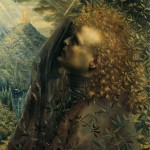
\includegraphics[width=.25\textwidth]{Parsifal-Delville-L-150x150.jpg}
\end{wrapfigure}

Our interpreter, T. Palamidessi\footnote{\url{http://en.wikipedia.org/wiki/Tommaso_Palamidessi}} echoes George Heart's interpretation\footnote{\url{http://www.amazon.com/Christianity-Dogmatic-Gnostic-Vivifying-Knowledge/dp/1412062284}} of Mouravieff:

\begin{quotex}
The times require the cooperation of all, and we offer a way which is safe, swift, direct, towards the overcoming of one's own moral, psychic, spiritual and biological states... Certainly the Catholic Church if it wanted to, without contradicting itself, could in modern times begin the second part of the mission, that of presenting the other face of Christianity, its esotericism, or, if you want, ``Christicism according to an archeosophical vision''. If once the great Clement of Alexandria stated ``I keep certain things under silence, by a willful choice, for fear of writing things which I have even avoided saying... .I would not give a sword to a child... (\emph{Stromata I, 1,14,3}), well, today the Church could break, albeit cautiously, this useless and harmful silence... .today it seems that the moment has come for us to speak, at least to a certain extent... \emph{Man on an earthly level has a thirst for truth, knowledge, freedom, total love and the spirit of self-preservation.} The same human bveing when he has the proof of his own survival, with all the implied consequences, then he will want to defend at all costs this survival in the best possible conditions, not as a wandering and confused spirit, now in a fleshly body in this world and now in the immense cosmic ocean of the Hereafter, but as a personal, deified I, which a the end of its days can depart safe and tranquil, not as an astronaut, but as a Theonaut, to land in the kingdom of Heaven where God has been waiting for Him always... 
\end{quotex}


He cites Ecclesiastes 12:6 as proof that man has a ``subtle body'' (also cited by George Heart):

\begin{quotex}
Remember Him before the silver cord is broken and the golden bowl is crushed, the pitcher by the well is shattered and the wheel at the cistern is crushed...
\end{quotex}

Hell is a real possibility for most humans.

\begin{quotex}
He who dies impure and not used to the scenery of the states after death, enters a world where he will be forced to experience the fears, the sufferings ad the desolation of limbo, of purgatory and of hell. In this new world an din its state of consciousness, even though the permanence is not eternal but transitory it is still full of risks, of dismay, and may give the impression of eternity. The risks consist of bewilderment, anguish, confusion and the inability to find the way leading to the Light of God. And then he will flee towards a new reincarnation as a way of escape, after a crisis between the states of sleep, dream, the frightening and accusing visions. Nor is there hope of being saved by the absolution and sacramental assistance of a priest, for those who have recourse to him, driven by fear of a divine punishment. Even though this help is a form of Initiation at the point of death, the dying person must have a preliminary religious preparation, both ordinary and extraordinary, exoteric and esoteric, and the education for the trials of the hereafter, already here in this life, while in full consciousness and vigor. The Redemption of Christ exists, but on condition to die Initiates.
\end{quotex}


The intelligence, writes Evagrius\footnote{\url{http://www.britannica.com/EBchecked/topic/236341/Gnostic-Centuries}}, lives in the heart, the thought in the brain.

Sin, also, is real, and not merely the construct of our mind. It has a metaphysical root.

\begin{quotex}
In conclusion, the forbidden fruit was not a sexual sin but an apostasy of Adam from God and the progressive yielding to the action of Karma, set into operation by him, which led him to walk and take the descending spiral of involution, then of evolution in the materialization.
\end{quotex}


Some struggle against this -- heroes, martyrs, mystics, saints and paramystics (adepts). Here is how ``monks'' do it:

\begin{quotex}
The athletes of ascesis and of exertion openly and directly measure their strength against devils, wiping them out so as to direct themselves toward the Adamitical homeland, Paradise.
\end{quotex}


All of this lies hidden, not merely in Christian tradition, but the Scripture itself.

\begin{quotex}
To who wins will be given to eat of the tree of life... who wins will not be harmed by the second death... to who wins will be given the manna... to who wins will be given the power over the nations... who wins will be dressed in white robes... who wins will be made a pillar... to who wins will be give to sit on my throne... who wins will inherit these things... 
\flright{\textit{Apocalypse of John}}
\end{quotex}


It is important to note that Palamidessi distances himself from magic in a way that Franz Bardon does not, explicitly.

\begin{quotex}
We have nothing to do with magic as commonly understood, which has already been damned by God, the Church, \& the honest... but always remember, the magician compared to God is humility incarnate, absolute trust, unquenchable Love, is a penitent Magdalene who washes the feet of the saviour, is Parsifal, in ecstasy, before the holy cup of the Graal.
\end{quotex}


In this, he follows Tomberg. However, this does not mean that the Christian mage or adept or paramystic has no ``means'' to work with, or is restricted to merely mental prayer:

\begin{quotex}
The icon can be considered a castle of meditation, a magic circle, a powerful means on which to fix the physical eyes and the eyes of the mind to isolate oneself from the profane world and enter into the sacred world. The images become supports for meditation. The holy image, whose use will be explained practically, fixed upon during meditation exercises, directs the will for the salvation of the devoted, and provokes a metaphysical experience. Iconognosis is a starting point for concentration, meditation and ecstasy. The image is dynamized, is animated, is filled with fluid like a pentacle, and performs deep, healthy transformations on the conscience. Archeosophical iconognosis is the most advanced form of ascesis through symbols. The icon concentrates, protects against distractions and temptations, and homologates the consciousness and the biological energies of the body to an archetypal icon formed by the Initiate and registered in the akashic plane.
\end{quotex}


Palamidessi argues that Christianity is intertwined with a ``more perfect Initiation'', one which is in essence the same as the pagan mysteries, but made more perfect (a principle enshrined in the New Testament, which perfects the Old). It is three-fold (to all three centers of man, properly identified even Scripture as Mind, Heart, Soul \& Strength, and is made easier by exoteric preparation through Christianity. It is ``undeniable that this initiation is typical of the Christians,'' who participate in a ``charismatic economy (administration of the gifts of grace) of the present, which throws open the doors to the Kingdom.''

Another source to confirm the claims of Palamidessi in regards to Christianity, both positively \& negatively, is Jean Borella\footnote{\url{http://books.google.com/books?id=fBLjJ_DWgFQC\&pg=PA68\&lpg=PA68\&dq=borella+diagram\&source=bl\&ots=ZGH73h-OJx\&sig=9uEolJjQqe5tyF384QuP0paAV3E\&hl=en\&sa=X\&ei=KyqST5HZDOPO2wXn47XpBA\&ved=0CCsQ6AEwAQ\#v=onepage\&q\&f=false}}. His diagram here can be compared to Soloviev's Law of Development\footnote{\url{http://www.gornahoor.net/?p=3571}}. Borella discusses how Gnostic became a dirty word within the Christian community, but how it properly belongs nowhere else.\footnote{Palamidessi proposed Out-of-body experiences, clairsentience/clairaudience, and the remembrance of past lives as spiritual experiments which could demonstrate with certainty that there was something beyond the material world. He dedicated his pamphlets that these quotes were taken from to ``Alexander, faithful defender \& friend of Origen, in memory of his martyrdom at Caesarea in Palestine, when in 250AD the anti-Christian persecution of Diocletian broke out. Rome, Sept. 29, 1968.}

To be continued...

\flrightit{Posted on 2012-04-20 by Logres}


\section{Palamidessi reads Evola}

There is an Italian commentary on, and reprinted text of, a letter from Evola to Tomasso Palamidessi here\footnote{\url{http://www.fondazionejuliusevola.it/Documenti/Evola_Palamidessi.pdf}}. Although this is not a translation, this is a rough survey of the contents of the letter, with a transliteration attempted at certain points, to convey or emphasize the meaning.

The commentator notes that the interactions between various schools, personalities in Italian esotericism was \emph{non sempre pacifici} (not always peaceful). Although Palamidessi's career has not been as well studied as Evola's, for obvious metaphysical reasons of ``heft'', this letter sheds a great deal of light. Palamidessi was born in Pisa in 1915, and moved to Turin at the age of 18, in 1933, having already demonstrated an interest in botany, astronomy, astrology, and medicine. After getting to Turin, he dedicated himself \emph{ad formazione occultista integrale} (to the formation of an integrated occultism). One of his teachers was the director of Museo Egizio, Ernest Scamuzzi. Around 1940, he had contact with Alfred Witte\footnote{\url{http://astrologer.ru/Witte/biography_eng.html}}`s Amburgo, as well as with Alexandre Volguine\footnote{\url{http://www.solsticepoint.com/astrologersmemorial/volguine.html}} (French astrologer), and some other personages connected with Masonry or Martinism -- Umberto Gorel Porciatti and Gino Witnesses. With the exception notably of astrology, all of his interests coincide with those of Evola's, and in fact, Palamidessi specifically replies to Evola's Man as Power (1926) \& Hermetic Tradition (1931)\footnote{\url{http://en.wikipedia.org/wiki/The_Hermetic_Tradition}} in pamphlets like The Erotic Power of Kundalini-Yoga (1949). Palamidessi's pamphlets, unlike Evola's metaphysically hefty tomes, have a technical, practical ``cut''. His debt to Evola is quite clear, when focusing on the content, and in some cases, Evola noticed a very real plagiarism. Palamidessi's doctrine follows closely three cardinal points of Evola:
\begin{enumerate}
\item Hermetism \& Alchemy are interpreted in light of tantric yoga

\item There is a hidden initiation thereby available to those who are ``not profane''

\item Tantric yoga is this path
\end{enumerate}

Palamidessi eschews a merely Theosophical orientation towards the ``subtle bodies'' (the lunar path).
\emph{Questa, quindi, la linea di pensiero comune} (This, therefore or thus far, is the line of common thought. The analyst points out that Evola and Palamidessi engaged in ripostes over time, and that Evola's final veredictum was formulated later:

\begin{quotex}
\textit{La donna assoluta non solo non possiede quell'Io, ma non saprebbe nemmeno che farsene, essa non sa nemmeno concepirlo e la sua presenza agirebbe in modo estremamente disturbatore presso a ogni genuina estrinsecazione della di lei più profonda natura.}
\flright{\textsc{J. Evola}, \emph{Metafisica del sesso}, Roma: Mediterranee 1958 , 1996, p. 179}

The absolute woman not only does not possess the ``I'', but she wouldn't even know what to make of it, she does not know how to conceive it, and its presence would act in an extremely disruptive manner in every genuine objectification of her deepest nature.
\end{quotex}


Palamidessi seems to have oscillated back and forth between ``explicit admiration'' for the author of such works he had borrowed heavily from, \& ardent criticism on this one point. Here is the untranslated Italian:


\begin{quotationx}
\textit{Siamo decisamente contro a tutti quei filosofi ed occultisti tanto ideologicamente nemici della donna da relegarla per molti secoli nel numero delle cose e degli esseri inferiori, laddove invece avrebbe potuto essere esaltata quale vivente espressione dell'Eterno femminino. Mi stupisce come un grande scrittore di esoterismo orientale della statura di Julius Evola ... abbia commesso il grave errore di negare alla donna il privilegio dell'immortalità e di quel principio che fa dell'uomo un essere superiore e imperituro. C'è proprio da chiedersi con quale criterio l'Evola abbia definito in un suo articolo sulla rivista Ignis (gen.-feb. 1925, n° 1- 2) ... ``la donna come cosa'' ... . L'uomo e la donna, di qualsiasi sviluppo morale e mentaleessi siano, non sono cose, ma individui, il cui livello evolutivo è tale da manifestare, o no, quel principio che fa dell'individuo un Dio. Ad ogni modo, questa mia constatazione ... non infirma affatto la mia simpatia di studioso nei confronti del dr. Evola che, se ha commesso degli errori di valutazione psicologica nei confronti della donna, ha pure dimostrato una profondità di vedute e di pensiero in altri settori della scienza occulta.}

We decisively oppose all those philosophers and occultists who are ideologically enemies of woman and relegate her for many centuries to be among things and inferior beings, when instead, she should be exalted as the living expression of the Eternal Feminine. It amazes me how a great writer of Eastern metaphysics of the stature of Julius Evola had created the serious error of denying to woman the privilege of immortality and of that quality that makes of man a higher and eternal being. It is proper to ask ourselves by what criteria does Evola define woman as a thing.

Man and woman, of whatever moral and intellectual development, are not things, but individuals, whose evolutionary level is such to manifest, or not, that principle that makes man a god. In every way, my thinking does not invalidate at all my scholarly sympathy toward Dr. Evola who, if he committed some errors of the psychological evaluation toward women, has only demonstrated a depth of insight and thought in other areas of occult science.
\end{quotationx}


It is only fair to note that Palamidessi had engaged in an extensive reading of Evola for years, up to and including virtual ``plagiarism'', as Evola himself at one point noticed (Guenon would later on comment, on the basis of reading excerpts that he was a ``charlatan'', although Evola seems to have wound up on equitable terms with Tomasso, both of whom died about the same time). Evola granted women the \emph{corpi sottili} (subtle body) but not the transcendental I, a position with roots in Weininger.

Here I can't help wondering if there was simply a blundering error on one or both of Evola or Palamidessi's part, over the wisdom application of a principle. The fact that great import or danger falls or turns on such a juncture should not amaze us. Here is an apocryphal\footnote{\url{http://creation.com/battle-quote-not-luther}} Luther quote --

\begin{quotex}
If I profess, with the loudest voice and the clearest exposition, every portion of the truth of God except precisely that little point which the world and the devil are at that moment attacking, I am not confessing Christ, however boldly I may be professing Christianity. Where the battle rages the loyalty of the soldier is proved; and to be steady on all the battle-field besides is mere flight and disgrace to him if he flinches at that one point.
\end{quotex}


And here we can intuit that although there is incredible danger of the ``Eternal Feminine\footnote{\url{http://www.bu.edu/arion/files/2010/03/Paglia-Great-Mother1.pdf}}'' being used in the Dark Age of the Kali Yuga to exalt chaos(as the virtuoso Paglia flirts with doing here) , that perhaps at the higher levels of debate, a very tragic misunderstanding can occur between those of deep insight. This may or may not be the case with Palamidessi.

In fact, it is an old Northern custom\footnote{\url{http://www.mun.ca/mst/heroicage/issues/9/forum2.html}} that a woman can act in the place of a fallen or absent male champion. Tolkien knew\footnote{\url{https://www.youtube.com/watch?v=MSNPeJAgBzo}} about this, and it puts one in mind of Deborah the judge, Esther the queen, and Judith the champion\footnote{\url{http://en.wikipedia.org/wiki/Book_of_Judith}}. The female is all the more potent for being forced to do violence to her sex and transcend it (in this case, taking the male place).

One is also tempted to wonder -- if Satan counterfeits ``traditional'' metaphysics by causing the resurgence of suppressed elements during the Kali Yuga, to the point of them achieving political power, wouldn't that mean he is counterfeiting something real, even in the feminine element?

It may be that Palamidessi, and Evola, as appeared to occur late in real life, can be reconciled.

\emph{More to come next week, with more transliteration from the letter, and with deference \& thanks to Cologero for suggestions.}


\flrightit{Posted on 2012-04-28 by Logres}

\begin{center}* * *\end{center}

\begin{footnotesize}
\begin{sffamily}
\texttt{Cologero on 2012-04-30 at 23:31 said:}

What can you conclude from the notion that a ``woman can act in the place of a fallen or absent male champion.'' The simply reinforces her secondary nature, doesn't it? How would we react to a man acting the the place of a fallen female? Wouldn't we consider that a lessening of his powers rather than an increase?

Why is the ``male gaze'' worthy of capital punishment? Is it simply because Thryth objects to it as a woman, or because she objects to it as queen?

You could have chosen a real example, rather than literary creations, e.g., St Joan of Arc.

I don't understand this: ``if Satan counterfeits ``traditional'' metaphysics by causing the resurgence of suppressed elements during the Kali Yuga, to the point of them achieving political power, wouldn't that mean he is counterfeiting something real, even in the feminine element?''

What elements are suppressed in the Kali Yuga? Doesn't a counterfeit always counterfeit something real? No one creates a knock off of a fake Rolex.

\hfill

\texttt{Cologero on 2012-04-30 at 23:43 said:}

Readers interested in the question about the ``I'' should read Chapter VIII in Weininger's \textit{Sex and Character}.

As for the link to the postmodern journal on Northern customs: there is no disagreement about a continuum of male and female characteristics. However, the point they miss, is that to define the continuum requires two significant pieces of knowledge. To ignore these, is tantamount to expecting a colour-blind man to define the visible light spectrum.

\begin{enumerate}


\item One must know what are the male and female characteristics.

\item One must know the two poles of the spectrum: absolute man and absolute woman.
\end{enumerate}


To try to define these empirically is to beg the question. The only solution is \emph{a priori}.

\hfill

\texttt{Aeneas on 2012-05-01 at 23:41 said:}

If Evola exaggerates the differences between man and women, it seems that Palamidessi wants to obliterate every distinction. What, then, is the male equivalent of the Divine Feminine, if not the Holy Spirit? Or put another way, the male is Purusha and the female Prakriti. But Purusha is Atman (the ``I''), so where does that leave Prakriti? Has Evola betrayed oriental metaphysics, or is he drawing a logical conclusion?

\hfill

\texttt{Charlotte on 2012-05-02 at 06:57 said:}

Holy Soul, the Shekinah, Bride of Christ

\hfill

\texttt{logres on 2012-05-04 at 06:32 said:}

Agreed concerning Joan of Arc. Journal chosen due to Tolkien's scene with the woman -- rather than being ``feminist'' or anti-tradition, it is a reaffirmation of male characteristics. What greater insult than to be beaten by, not the king, but his little daughter? However, there is something ``more'' in Christianity than Evola gives in relation to sex; Evola never discusses to what extent the upsurge of chaos \& the female are actually in contingency with the divine plan; our alternatives are not Evolutionary view vs. Evola. I realize most people here know that, so it was a cheap point. I should concentrate on discerning more along the lines of Charlotte's comment, which was where I am headed. To that end,

\url{http://www.kober.com/marriage.php}

Bo-Yin-Ra

Also, Mouravieff's comments about the knight and his true lady who advance step by step up the stairs of the divine Solfeggio notes in Gnosis obviously is speaking of ascetic practices within and outside marriage designed to realize the Eternal Union of the separated poles. I'll try to excerpt this more directly very soon.

\hfill

\texttt{logres on 2012-05-04 at 06:34 said:}

Palamidessi has a pamphlet directly concerning occult characteristics of the male \& female, so I won't comment anymore on him till after I have obtained \& read.

\hfill

\texttt{Charlotte on 2012-05-04 at 20:13 said:}

essay here you may or may not find interesting, talking about Guenon's astrology, end of Kali Yuga, shift from polar to solar etc

\url{http://www.alignment2012.com/polar-to-solar.html}

Cx

\hfill

\end{sffamily}
\end{footnotesize}


\section{General Law}

After finishing \emph{Gnosis 1,2,\&3}, the concept of \textbf{General Law} stands out as very nearly the most important paradox in the book we can grasp, if we want to grasp daily practical implications. This concept has political implications, as well as personal: No one escapes General Law -- it is impossible. In the words of Phillip Dick in the novel V.A.L.I.S.\footnote{\url{http://en.wikipedia.org/wiki/VALIS}}, ``those who fight the Empire, become the Empire (the Black Prison)''. Or if you prefer Saint Paul, ``we struggle not against flesh and blood... bodily exercise profiteth little... we are in the world, but not of it... ''. General Law is the daemonic/angelic/demonic hierarchy which determines natural history and cosmology, as well as the fate of the person who is ``under the Law''. Now, for Saint Paul, the law is ``holy and good'', yet it is ``\emph{given} for the lawbreaker''. One might say, it is \emph{a given}. But Mouravieff does more, and attempts to explain the inner workings of this law. For instance, how can it be both good \& evil? What does Saint Paul intend to teach, here? We are knee-deep in the mysteries of the epistles with this teaching. One principle is worth mentioning as an aside: The General Law allows you to escape it \emph{only if you train (or create/provide for) your replacement}. All sorts of applications could be made here, for instance, with the duty to raise children, or a master teaching a pupil.

This Law is iron -- the more one attempts to confront it with human means in space and time, the more powerful the Law becomes. It grows through defiance. This is the existential defeat and despair of fallen man, and it is, coincidentally, \emph{precisely what the illusory dream of Revolution is truly all about}. Man will confront the cosmic tyrant and break his chains. Man will stand against the gods, on behalf of all of our sorrow, rage, fear, suffering, and hunger. Many would portray Christ as the new champion of this. And man will thereby strengthen Satan.

But what did King David\footnote{\url{http://www.biblegateway.com/passage/?search=Psalm+2\&version=KJV}} see of this?

\begin{quotex}
Why do the heathen rage, and the people imagine a vain thing?

\textsuperscript{2} The kings of the earth set themselves, and the rulers take counsel together, against the Lord, and against his anointed, saying,

\textsuperscript{3} Let us break their bands asunder, and cast away their cords from us.

\textsuperscript{4} He that sitteth in the heavens shall laugh: the Lord shall have them in derision.

\textsuperscript{5} Then shall he speak unto them in his wrath, and vex them in his sore displeasure.

\textsuperscript{6} Yet have I set my king upon my holy hill of Zion.

\textsuperscript{7} I will declare the decree: the Lord hath said unto me, Thou art my Son; this day have I begotten thee.

\textsuperscript{8} Ask of me, and I shall give thee the heathen for thine inheritance, and the uttermost parts of the earth for thy possession.

\textsuperscript{9} Thou shalt break them with a rod of iron; thou shalt dash them in pieces like a otter's vessel.

\textsuperscript{10} Be wise now therefore, O ye kings: be instructed, ye judges of the earth.

\textsuperscript{11} Serve the Lord with fear, and rejoice with trembling.

\textsuperscript{12} Kiss the Son, lest he be angry, and ye perish from the way, when his wrath is kindled but a little. Blessed are all they that put their trust in him.
\end{quotex}


The General Law \emph{is the missing link} between the testaments of Law \& Grace. Jesus, also is, because he satisfied that General Law, and thereby provided an opening. But the Law is not dead, but is active and alive still, unless one is under the aegis of some symbol. It is also a warning to Modern Times: the power of the angels will only bind our chains tighter if we presume to liberate man in any other way than the one way given, the narrow way. This way is to transcend the human condition, through vertical energies, \& to enter the Kingdom of Heaven. There is no other way which the Guardians of the Threshold\footnote{\url{http://en.wikipedia.org/wiki/Guardian\_of\_the\_Threshold}} will permit, personally or collectively. As seductive as the idea of building everyone a duplex with running water and free phone lines is, it is actually a grave sin against every human being \& one's own soul to directly confront the Guardians of the General Law with human desire and physical means, \emph{promoting the Revolution on earth}. Revolution will only build more Revolution, because it will only build the Black Prison higher and stronger. I will repeat this -- to directly confront the hierarchies in a human and physical (read ``political'') manner is to spit in Christ's face (who Himself refused this temptation, though he might have done it for his own sake). Ultimately, all Revolutionists are building their own Hell, and it will be all the more secure for that, since they built it, who imagine that anything in this life on its own level can ``save'' man, political or otherwise.

In fact, as Luther apocalyptically\footnote{\url{http://creation.com/battle-quote-not-luther}} said, it is the gravest sin in the world today, because this is the occult point of attack:

\begin{quotex}
If I profess, with the loudest voice and the clearest exposition, every portion of the truth of God except precisely that little point which the world and the devil are at that moment attacking, I am not confessing Christ, however boldly I may be professing Christianity. Where the battle rages the loyalty of the soldier is proved; and to be steady on all the battle-field besides is mere flight and disgrace to him if he flinches at that one point.
\end{quotex}


The Moderns are traitors even to their founding saint, as the above amply illustrates; sadly for them, Luther may be saved anyway, but they will not, because God will laugh them to scorn and mock them, and Christ Himself will break them in pieces. Christ permits the General Law, because He himself satisfied it, and has directed in what manner it may be overcome. It is \emph{hubris}\footnote{\url{http://en.wikipedia.org/wiki/Hubris}} to imagine another way.

There is a warning for traditionalists also -- the Gods of these times permit the modern excess in an open manner, and thus to directly confront this in an overly physical manner is to become guilty of the same modern \emph{hubris} the Moderns practice (think the Confederate States of America, here). Rather, warn those who need warning, \& save yourselves, first, and allow Revelation and history to unfold until ``it is time''. Do not confront Satan directly (for even the archangel Michael did not\footnote{\url{http://www.biblegateway.com/passage/?search=Jude+1\%3A9\&version=KJV}}), for the power of evil has not yet been exalted. This is the Kali Yuga. This is why the founders of Gornahoor have spent so much time on ``theory'' and personal practice, rather than ``direct action'', although one can certainly prepare the groundwork and framework against the chaos that is sure to inevitably transpire.

Instead, we should spend our excess power and time in seeking to legitimately (read, traditionally) escape General Law in the approved manner, through the narrow gate. The jealous and all powerful (within their spheres) hierarchies seem to give man much ``leeway'' but it is actually a total illusion, designed to keep him in chains to further the Common Good and destiny of the species, rather than liberate his soul prematurely. Man is so fragmented and insane, spiritually, that God permits him to be ruled with illusion and lies in order that this generation will perish in ``feeding the moon'' (see Gurdjieff's teachings), but that the Divine Plan will go on. Man will think himself free under the Revolution -- the Revolution is a deepening of the Lie to its most powerful point to counterbalance the excess of disintegrative energies that is loose in our time.

And he will die and perish, and his states and societies will perish with him, because Man is more important than he dreams, or than even the Revolution promises. Man will endure anyway.

Even the Demons delight in the Great Game, but they secretly yearn for heroes who are equal to tilt the course against them, teaches Mouravieff. Is this what you, too, desire? Then bow down in the temple of Rimmon, \& repent of speaking ill of high authority, with all of its attendant woes and evils, and seek the narrow gate. Reject Revolution, embrace Authority; submit, and bow down in the temple of Rimmon\footnote{\url{http://en.wikipedia.org/wiki/Naaman}} if you have to, but pray without ceasing to the Illuminator of the Heart, that you might defeat the adversary, and be set free eternally. This is the meaning of the saying, \emph{if the Son makes you free, you shall be free indeed}.

But for those who resist, the Absolute III and the energies of the occult servants of the Holy Spirit will devour them.

This, and much more, is taught in Mouravieff's \emph{Gnosis}.


\flrightit{Posted on 2012-07-13 by Logres}

\begin{center}* * *\end{center}

\begin{footnotesize}
\begin{sffamily}
\texttt{apeiron on 2012-07-14 at 17:20 said:}

Nice, but that link you provided to Luther's famous battle quote argues against the legitimacy of it. The quote was attributed to him in a fictional 19th Century novel by Elizabeth Rundle Charles however poetic it may sound. Luther would have done well to follow his own advice had he not come so late to the Jewish question, but by then the Revolutionary Reformation had blown full swing and Europe was dangerously partitioned with disastrous future consequences to follow.

Particularities aside, and to simply take what the essence of the message you are trying to convey on an objective level this is what we conclude: Don't fight the Satanic forces of the Kali-Yuga head on, (as to do so would bring the wrath of the Zeitgeist/Universal/General Law which at this point in time favors the Adversary) but instead form an elite of the few who remain awake in the night to save your own asses from the last judgement and to hell with the rest of the goyim. I'm still trying to figure where the heroic part comes in. Did Christ not incur this wrath under crucifixion(perhaps as initiation)? Did not the Iron Guard and so on?

The old' days still had men worthy of a higher caliber to oppose it, because despite all, the essence of that opposition carried a spiritual significant meaning that rings true to us.

\hfill

\texttt{logres on 2012-07-14 at 22:17 said:}

For the sake of clarity, your construal is not what I intend to mean. Saving yourself has nothing to do with it. Since I've just lost two lengthier replies, I'll content myself with noting that Mouravieff's concept of Authority in consonant with Tradition, \& that the issue here is: What are you capable of forcing the General Law to concede? I am not discouraging anyone who is capable from acting; what I wish to avoid is encouraging those who think that there is no warning here for us, as well as the Revolution.

\hfill

\texttt{logres on 2012-07-14 at 22:22 said:}

You fight spiritually just as you would physically -- using an Art of War, rather than acting without a precise knowledge of times and seasons, inner or outer. I am not trying to discourage that, but rather note that there is a warning here to us all. It was a point I did not want to make, but thought that knowledge and logic from the doctrine of General Law required be made. That's certainly not the last word on the subject, and would require another assay.


\hfill

\end{sffamily}
\end{footnotesize}


% Sección para Clemente?
\section{The Golden Book \& Saint Clement}

Boris Mouravieff, when teaching on polar-beings in \emph{Gnosis}, references the existence of the Golden Book, an oral (if also incomplete) compilation of Jesus' teachings to the inner circle of disciples. It is only fair to point out that (like the exoteric-esoteric paradox of Christianity itself), the idea of a written compilation of oral teachings is somewhat odd -- nevertheless, then, its very incompleteness testifies to its legitimacy, as some teachings must be ``discovered''.

Clement of Rome\footnote{\url{http://www.scribd.com/doc/13561289/-The-Authentic-Peter-The-Preaching-of-Simeon-Kefa-from-the-Journal-of-T-Flavius-Clemens-Clement-The-Clementine-Recognitions-Recognitions-of-Cl}} was involved in the ``inner'' circle of disciples following Christ's death -- the ``inner'' circle perpetuated itself and thereby endorses the reading of the Gospels in this light: Jesus' parables are given because ``they have ears to hear, eyes to see, but cannot... ''. A \emph{parable} (as Ea points out in the collected Ur-group writings) is a ``carrying with or beside'', and thus less direct than a \emph{symbolon}, which is a ``carrying into''.

\begin{quotex}
Clement was a highly educated young man \emph{with a photographic memory}. He was also a member of the powerful Flavian dynasty (and cousin to emperors Vespasian, Titus and Domitian). Though young, he was a man of considerable financial means. He had no background whatsoever in Judaism and would not have come into the circle of Nazoreans in Jerusalem had he not by chance net Barnabas in Rome and followed him to Palestine.Clements high intellect and great curiosity were not lost on James the Just (Yaakov haZaddik), overseer of the Nazorean Assembly in Jerusalem. He officially assigned Clement to Peters group of students and commanded Clement to send periodic reports of Peters activities back. These reports are often mentioned in the book, and are sometimes indistinguishable from Clement s own journal entries. As an unbaptized gentile proselyte, Clement and others were not allowed to eat or sleep with the baptized until judged spiritually and doctrinally fit for immersion.
\end{quotex}


I am not sure his relation to Clement of Alexandria, a point I raised in a previous essay when using this source. Jackson Snyder appears to confuse the two Clements, unless (perhaps) they were actually related by blood as well as by body of myth and name. Regardless, Clementine literature\footnote{\url{https://en.wikipedia.org/wiki/Pope\_Clement\_I}} portrays him (and Clement of A) as:

\begin{quotex}
the Apostles' means of disseminating their teachings to the Church
\end{quotex}

I will remark here, two things: the presence of an elite (``highly educated... with a photographic memory'') and the doctrine of secret teaching (the ``Church'' was a cult tolerated by the disciples as a condescension to man's weakness, but a body which was subjected to impulses from an elite to ``regulate'' it's health).

The beginning of the text rings true:

\begin{quotex}
I Clement, who was born in the city of Rome, was from my earliest age a lover of chastity; while the bent of my mind held me bound as with chains of anxiety and sorrow. For a thought that was in me whence originating, I cannot tell constantly led me to think of my condition of mortality, and to discuss such questions as these:Whether there be for me any life after death, or whether I am to be wholly annihilated: whether I did not exist before I was born, and whether there shall be no remembrance of this life after death, and so the boundlessness of time shall consign all things to oblivion and silence; so that not only shall we cease to be, but there shall be no remembrance that we have ever been. This also I revolved in my mind: when the world was made, or what was before it was made, or whether it has existed from eternity. For it seemed certain, that if it had been made, it must be doomed to dissolution; and if it be dissolved, what is to be afterwards? Unless, it may be that all things shall be buried in oblivion and silence, or something shall be, which the mind of man cannot now conceive.
\end{quotex}


What noble young man, starting upon life, who is not clouded in the fogs of lust, has not felt this yearning? At first, Clement desires to consult a magician who will raise a spirit from the dead to prove the immortality of the soul, but a friend dissuades him, saying that the Elohim set themselves against those who trouble dead souls (here in the idea/reality of General Law).

He defends a visitor to Rome who tries to speak on behalf of the disciples, and invites him to his home. Clement sails to Caesarea, and there is brought to meet Kefa (Peter). Peter has decided to ``choose'' him as his successor. Peter teaches him the cause of man's ignorance:

\begin{quotex}
The will and counsel of YHWH has for many reasons been concealed from men; first, indeed, through bad instruction, wicked associations, evil habits, unprofitable conversation, and unrighteous presumptions.~ On account of all these, I say, first error, then contempt, then infidelity and malice, covetousness also, and vain-boasting, and other such like evils, have filled the whole house of this world, like some enormous smoke, and preventing those who dwell in it from seeing its Founder aright, and from perceiving what things are pleasing to Him. What, then, is fitting for those who are within,excepting with a cry brought forth from their inmost hearts to invoke His aid, who alone is not shut up in the smoke-filled house,that He would approach and open the door of the house, so that the smoke may be dissipated which is within, and the light of the sun which shines without may be admitted... 
\end{quotex}


Peter is saying here, that the Kali Yuga predominates. This poetic metaphor resonates even with Western ecclesiastical\footnote{\url{https://en.wikipedia.org/wiki/Edwin\_of\_Northumbria}} history:

\begin{quotex}
The present life man, O king, seems to me, in comparison with that time which is unknown to us, like to the swift flight of a sparrow through the room wherein you sit at supper in winter amid your officers and ministers, with a good fire in the midst whilst the storms of rain and snow prevail abroad; the sparrow, I say, flying in at one door and immediately another, whilst he is within is safe from the wintry but after a short space of fair weather he immediately vanishes out of your sight into the dark winter from which he has emerged. So this life of man appears for a short space but of what went before or what is to follow we are ignorant. If, therefore, this new doctrine contains something more certain, it seems justly to deserve to be followed.''
\end{quotex}


The souls of Edwin and Clement were worthy to receive the Truth, \emph{therefore, it appeared}. Those who think all souls are equal are servants of Satan -- all souls are in one sense equally valuable, but there is a reason certain people yearn towards the truth, and others do not. Clement desires very much to know the answers to his questions, enough to humble himself (outwardly and inwardly) -- this ``creates'' a higher Truth for him than his current spiritual state has manifested (the true un-Semitic definition of humility).

Simon Peter prepares for an upcoming controversy with Shimon the Magus, which is delayed, giving them time to discuss things which may come up during the debate. Clement is somewhat saddened, but Peter teaches a truth similar to Boethius' arguments in \emph{Consolatio}:

\begin{quotex}
He who believes that the world is administered by the providence of YHWH El Shaddai ought not, O Clement, my friend, to take it amiss, in whatever way particular things are done, being assured that~ of YHWH guides to a favorable and fitting issue even those things which seem superfluous or contrary in any business, and especially towards those who worship Him more intimately; and therefore he who is assured of these things, as I have said, if~anything occur contrary to his expectation, he knows how to drive away grief from his mind on that account, holding it unquestionable in his better judgment, that, by the government of the good YHWH,even what seems contrary may be turned to good.
\end{quotex}


Peter sees an opportunity to expound oral teaching, which cannot be taught any other way, including \emph{Sola Scriptura}.

\begin{quotex}
for I believe that it has been done by the providence of YHWH,for your advantage; that I may be able, in this interval of seven days,to expound to you the method of our faith without any distraction, and the order continuously, according to the tradition of the Navi Emet, who alone knows time past as it was, the present as it is, and the future as it shall be: which things were indeed plainly spoken by~Him, but are not plainly written; \emph{so much so, that when they are read, they cannot be understood without an expounder, on account~of the sin which has grown up with men,} as I said before.
\end{quotex}


This is absolutely true for all except those of whom the mystery of the Just applies, and it still affects them. Peter teaches a truth which resonates with Guenon's work on the Manifest/Unmanifest:

\begin{quotex}
There always was, there is now, and there ever shall be, that by which the first Will begotten from eternity consists; and from the first Will precedesa second Will. After these came the world; andfrom the world came time: from this, the multitude of men; from the multitude the election of the beloved, from whose oneness of mindthe peaceful Malkuth of YHWH is constructed... 
\end{quotex}

In other words, there is something underlying God's manifestation that is unmanifest. The Orthodox still distinguish between God's essence (unknowable) and His energies (manifested and experienced). Peter then teaches about the ``upper waters'' which divide heaven and earth. The point here is that Peter is \emph{initiating} Clement. We learn about Nimrod and the worship of fire, as well the adoration of each nation's \emph{sarim}\footnote{\url{http://www.archangels-and-angels.com/misc/sarim.html}} as gods. Here is given the rudiments of a cosmology. The Western tribes drove the middle tribes into the East by means of violent warfare. Abraham the astronomer recognizes the Creator in the stars and is taught by the angel of the Lord, who shows him that his inheritance lies in Palestine (where usurpers dwell). This is connected with the ``boundaries of men'' set by the \emph{sarim} and General Law. What follows is a summary of the Old Testament. Then comes the Advent. It is worth noting that the 12 disciples and 70 elders mirror the angelic orders, in the intention of Christ, the image of the \emph{Imperium}:

\begin{quotex}
When Elohim had made the world, as Master of the universe, He appointed chiefs over the several creatures, over the trees even, and the mountains,and the fountains, and the rivers, and all things which He had made,as we have told you; for it were too long to mention them one by one. He set, therefore, a malach as chief over the malachim, a spirit~over the spirits, a star over the stars, a demon over the demons, a bird over the birds, a beast over the beasts, a serpent over the serpents, a fish over the fishes, and a man over men, who is Moshiach Yeshua. But He is called Moshiach by a certain excellent rite of obedience; for as there are certain names common to melekim, as Ahashwerosh among the Persians, Caesar among the Romans,Pharaoh among the Mitsrayim, so among the Yahudaïm a melek is called Moshiach. And the reason of this appellation is this: Although indeed He is the Son of YHWH, and the beginning of all things, He became as man; Him first YHWH anointed with oil which was take from the wood of the tree of life: from that anointing therefore He is called Moshiach... \end{quotex}


We also learn that the schisms of the Judaic sects were work of the devil to obscure the truth, and that baptism was a Christian rite because man is ``taken from the waters'', as the chosen one is. More teaching is given about the internal disputes of Jewish sects, including Saul and John the Baptist. After James is thrown down the steps of the Temple by Saul, and persecution breaks out, Peter is sent to Caesarea to refute Shimon Magus, who is misleading many of ``our people'' by pretending to be the Primordial man come again -- the Messiah. Peter thus weaves divine history into a personal narrative of why Clement and he are there in the city.

\emph{More of Clement and Peter, to come... .}



\flrightit{Posted on 2012-08-04 by Logres}


\section{Clement’s Initiation: Peter and Shimon Magus debate}

This is a continuation of a previous post\footnote{\url{https://gornahoor.net/?p=4533}}. My source document is here\footnote{\url{http://www.scribd.com/doc/13561289/-The-Authentic-Peter-The-Preaching-of-Simeon-Kefa-from-the-Journal-of-T-Flavius-Clemens-Clement-The-Clementine-Recognitions-Recognitions-of-Cl}}, and I have already noted the problems with dates -- it is part of the Clementine literature, involving at least two Clements, but its contents are noteworthy.

Simon Magus is an under-appreciated character, even though modern sensibilities have tried to paint him as someone who fights poverty or performs tricks as good deeds -- instead, he is a pivotal figure in the history of the Church.

To continue, Peter (Simon Kefa) is recounting the Apostles' arguments with certain Jews, in which Matthew and Phillip both speak, along with James the Just:

\begin{quotex}
Then a certain Prush, hearing this, chided Philippos because he put Yshua on a level with Moshe. To whom Natanyahu bar Talmai,answering, boldly declared that we do not only say that Yshua is equal to Moshe, but that He is greater than he, because Moshe was indeed a navi, as Yshua is also, but that Moshe was not the Moshiach, as Yeshua is, and therefore He is doubtless greater who is both a navi and the Moshiach, than he who is only a navi. After following out this train of argument, he stopped.
\end{quotex}

Here we see (early on) the Christian claim to primacy which caused such trouble within the religion of Judaism (and in Rome). However, it was also more complex than this, as Peter will explain. James the Just actually argues that Jesus ratifies the angels, rather than the other way around, and Mathias (in place of Judas), claims that (in any case) the Messiah is worthy of great love, no matter what one thinks. Each apostle makes a uniquely personal and uniquely intelligent argument:

\begin{quotex}
After him Yosef bar Naba, who also is called Mattityahu, who was substituted as a Shliach in the place of Yahudah of Keriot, began to exhort the people that they should not regard Yshua with hatred, nor speak evil of Him. For it were far more proper, even for one who might be in ignorance or in doubt concerning Yshua, to love than to hate Him. For YHWH has affixed a reward for loving and a penalty for hating. For the very fact, said he, that He assumed a Yahudai body, and was born among the Yahudaïm, how has not this incited us all to love Him? When he had spoken this, and more to the same effect, he stopped... 
\end{quotex}


The apostles argue that the Messiah is heaven-born, otherwise, John the Baptist would truly be the greatest born of women, and thus Messiah, rather than Jesus. It's a very interesting look inside the ``sects'' of Judaism at that time. Indeed, Gamaliel is said to secretly be a follower of Christ, who remained within Jewish ranks in order to moderate their fury, which he does, giving his famously pragmatic speech ``If these things be of God... ?''. James proceeds, and has almost convinced everyone to receive baptism when Saul intervenes with agitation and violence, and James is cast down the temple steps and left for dead.

Peter says he fled to Jericho, then Caesarea, and intends on going to Rome following the debate with Shimon Magus. No women are present at the debate, and Peter opens by explaining his practice of night-time meditation, which Clement approves of:

\begin{quotex}
I believe, therefore, that you also have acquired the habit of wakefulness, as you state; and you have wished at a fitting time to explain this to us, that we also may not grudge to throw off and dispense with some portion of our sleep, that we maybe able to take in the precepts of the living halakah. For when the food is digested, and the mind is under the influence of the silence of night, those things which are seasonably taught abide in it.
\end{quotex}


Peter wants to know what character Shimon is, that he might know how to argue without casting pearls before swine. Niceta warns them (he was once a co-worker with Shimon):

\begin{quotex}
but because I well know the impieties of this man, I think of your reputation, and at the same time the inner-beings of the hearers, and above all, the interests of the truth itself. For this magician is vehement towards all things that he wishes, and wicked above measure.
\end{quotex}


The description sounds like a high ranking initiate:

\begin{quotex}
This Shimons father was Antonius and his mother Rachel. By tribe he is a Shomroni from a village of the Get tones; by profession a magician yet exceedingly well trained in the Greek literature;desirous of glory, and boasting above all the human race, so that he wishes himself to be believed to be an exalted power, which is above YHWH the Creator, and to be thought to be the Moshiach, and to be called the Standing One. And he uses this name as implying that he can never be dissolved, asserting that his flesh is so compacted by the power of his divinity, that it can endure to eternity. Hence,therefore, he is called the Standing One, as though he cannot fall by any corruption... \end{quotex}

Shimon has replaced Dositheus\footnote{\url{https://en.wikipedia.org/wiki/Dositheos\_\%28Samaritan\%29}} as head of the thirty, and taken Luna as a consort; he also uses the dead spirit of a boy to accomplish his ``miracles''. In fact, he even explains to Niceta how it is done, by adjuring Malakim to allow a spirit to come back. Peter is moved to tears, and says that spirit of the boy of air is not what it seems to be:

\begin{quotex}
But, in truth, he is deluded by demons...
\end{quotex}


\emph{Incidentally, Bo Yin Ra claims that ``lemurian physical entities of putrefaction'' use people's souls to create illusions of human spirits for their own energetic purposes, in perfect agreement with Peter}. Peter answers objections to God's goodness in exposing man to the Kali Yuga, when almost all men are lead astray -- he does so simply by teaching that God permits it to reveal who are truly His. \emph{Clement is asked to leave, prior to Shimon's actual arrival, because he has not yet been baptized, and Peter needs to enter God's presence for prayer.}

Shimon arrives and challenges Peter, refusing \emph{Shalom}. Peter attempts to show what he meant: that the inquiry would be peaceful and quiet, not violent and contentious. Shimon shoves this aside, and says Jesus came to bring a sword, not peace; Peter joins battle and quotes the peacemaker beatitude. The conflict begins in earnest. Peter ends up saying ``do not rashly take exception to things you do not understand'' quite a lot. Shimon shows his hand, and argues that Christ contradicted himself (after it is clear that Peter actually has lived with Jesus long enough to know what he is talking about). They swap rhetorical acrobatics over Jesus' saying about ``dividing a house'' and Peter comes off as very well-spoken, although not as naturally so as Shimon, who appears to be merely squabbling over rhetorical terms. In a somewhat ``modern moment'', Peter tells Shimon not to speak of what the learned or unlearned are willing to believe, \emph{but what he Shimon really thinks of the navi}, Christ, whose Gospel Peter is compelled to teach authoritatively. Shimon presents his creed of many elohims, with one above all: ``\emph{elohim hagadol of elohim}``. Shimon teaches that the Jews were ignorant of him, and Peter insists that the Creator YHWH is indeed this very Elohim of Elohims.

We are in the middle of the birth of Gnosticism, here.

Peter answers by claiming that all \emph{malachim} (godlike angels) are messengers to the tribes of men:

\begin{quotex}
For every tribe has a malach, to whom YHWH has committed the government of that~tribe; and when one of these appears, although he be thought and~ called elohim by those over whom he presides, yet, being asked, he does not give such testimony to himself.
\end{quotex}


The Bible is not anti-polytheistic, but henotheistic\footnote{\url{https://en.wikipedia.org/wiki/Henotheism}}. \emph{See Galatians: angels are tutors}. Peter claims that the \emph{malachim} are appointed of God, and sometimes a mortal man is chosen instead, but that the worship that goes to them is carried to God. Of course, Shimon thinks this is a delusion: there is a hidden Elohim that no one knew until now; YHWH is deluded, self-deluded, into thinking He is the true Creator; only the enlightened ones can escape this delusion and go to join the true Elohim. He cleverly quotes Christ -- ``No man has known the Father, but the Son... ''. Moses, then, and all the rest, were ignorant of true Elohim. When Peter points out that Shimon doesn't believe in Christ's sayings, and that Moses prophesied of Christ (and therefore, accepted Christ's pre-eminence and was not entirely ignorant of truth as claimed), Shimon points out that ``having a Son'' involves the Creator in passions. Familiar ground, but freshly done in this exchange. Shimon (like many Gnostics) is very slippery here. Or subtle, depending on your loyalty. The rest of the debate is quite interesting, and very complex, very rhetorically brilliant on both sides (another reason I think the letter is genuine). It prefigures the great Gnostic-Christian divide of those early centuries quite well; this encounter may have symbolically actuated the great divide. Suffice it to say there are many strokes of genius by Peter as well as Shimon; Peter asks why the immortal, invisible New Power does not confer a new sense on men to recognize him, and if He has given it to Shimon, then why not to them? And can Shimon read their thoughts, since he can read God's? Predictably, Shimon argues that he learned from the Bible's own story that the ``Creator'' cannot be good -- He made a manifestly imperfect world. Thus, the Problem of Evil undermines faith in the ``Creator''. Peter mocks the rejection of Torah on the basis of Torah, but Shimon frames the \emph{Euthyphro} problem brilliantly and classically:

\begin{quotex}
But even if Torah had not given indications from which it might be gathered that the Elohim who made the world is imperfect, it was still possible for me to infer from those evils which are done in this world, and are not corrected,either that its creator is powerless, if he cannot correct what is done amiss; or else, if he does not wish to remove the evils, that he is himself evil; but if he neither can nor will, that he is neither powerful nor good. And from this it cannot but be concluded that there is another \emph{elohim} more excellent and more powerful than all. If you have aught to say to this, say on... .
\end{quotex}


Peter of course does say on. He not only counters with a very traditional statement about choosing wise instructors:

\begin{quotex}
O Shimon, they are liable to conceive such absurdities against YHWH who do not read Torah with the instruction of masters, but account themselves teachers, and think~that they can understand Torah, though he has not explained it to them who have learned of the Master.
\end{quotex}


... but uses a \emph{reductio ad absurdum} to show that the Ineffable light lies under the same charge brought against the ``Maker'' or ``Architect''. They are now at the very heart of the matter, metaphysically speaking, and all those who wrestle today\footnote{\url{http://www.scribd.com/doc/57492796/Gnostic-Fragments-by-Nimrod-de-Rosario}} between accepting Gnostic doctrine or Christian tradition (or any other) would do well to ponder this collision, so vividly painted in the ancient literature.

We will end this post with Peter's objection to the Ineffable God, which is one of the strongest I have seen:

\begin{quotex}
Whence that new power of yours is not only found liable to a similar charge, but even to a worse one, if, in addition to all these things, it is believed to be, when it is not. \emph{For He who created the world, His existence is manifest by His very operation in creating the world, as you yourself also confess. But this power which you say that you alone know affords no indication of itself, by which we might~perceive, at least, that it is, and subsists.}
\end{quotex}


\emph{More to come later, about the continued journey of Clement with Peter, and the initiation of Clement, which Peter says he did ``moved by certain unknown motions of the heart''.} Also, the notes of Tomberg on Cyprian the Mage\footnote{\url{http://en.wikipedia.org/wiki/Cyprian\_and\_Justina}} are worth reading --- the magic that was being done was not a ``joke''.


\flrightit{Posted on 2012-08-11 by Logres}

\begin{center}* * *\end{center}

\begin{footnotesize}
\begin{sffamily}
\texttt{Gabe Ruth on 2012-08-13 at 15:43 said:}

Thank you for the posts.

I mentioned it in a recent comment so I hesitate to bring it up again, but have you read A Voyage To Arcturus? That is a vividly painted portrait of Gnosticism, and I truly wish I'd never read it.

The question those who wrestle with these options must answer is whether you would give your allegiance (for whatever that's worth) to a good but not all-powerful God if there was a higher power that was not good, and whether it would make a difference if the non-omnipotent good God was your creator. I've never been particularly worried that atheists are right, but the gnostics trouble me, because their answer to the problem of evil seems so reasonable.

This piece also got me to thinking about Voegelin's use of the term gnostic, and a way to unify his meaning with the historical gnostics: they both posit a way of being, a new truth, which is wholly opposed to everything that we see around us and have inherited from our ancestors, in fact casting the old ways as completely evil, the source of the evils that we now experience.

\hfill

\texttt{logres on 2012-08-13 at 16:03 said:}

I saw your comment on Arcturus (I think) because I looked the book up -- Lewis uses it for his space trilogy, so I marked it to buy and read, at some point, thank you. The Gnostics trouble me more than atheists, likewise -- as an acquaintance pointed out, the lesson of Gnosticism may be ``let the dead bury the dead'' -- sometimes traditional forms have to be resurrected rather than resuscitated (if that's a good analogy?). Which means a lot of hard work. And they can certainly help us in dealing with the current climate (which is actually becoming very Demiurgic, what with the rampant PC and reigning gods of multicult, etc.). If the Gnostics had the courage to go against God, what excuse do we have for not standing against false gods? They certainly have praiseworthy points. I chose the debate because Peter's answers are so good -- if the Demiurge really is real, and ``revelation'' is from him, how does this get the Ineffable off the hook for the problem of evil? It doesn't (it seems to me) -- it just pushes the problem back by giving an emotionally charged and short-term satisfying answer (defers the cost). Same as atheism with final causes.

\hfill

\texttt{Dominion on 2012-08-14 at 00:14 said:}

Professor James Cutsinger provides a good explanation of the role of the exoteric ``religion'' in his lecture entitled ``The Noble Lie'', available on youtube. Taking this viewpoint, it is not so much the religion, be it Christianity or Gnosticism, that matters, so much as it is the potential of its use as a spiritual aid. The doctrine of the Triune God and the creation undergoing apotheosis and the doctrine of the Demiurge and the ``true Light'' or ``laughing Christ'' can be taken as conflicting narratives being used to attain the same end, at which point the doctrines themselves (their `literal' truth or untruth not being the point) can be surpassed and salvation or liberation attained. In that respect, the initiate among the Cathars and the one receiving the Eucharist at Divine Liturgy or Mass can embrace each other as brothers in a sense beyond their fellows in the exoteric faith. That said, Gnosticism's ability to be of much use as a faith on which civilizations can be founded seems limited, precisely because of its ambivalence to matter and the material world.

Also, at what point do you believe that Traditional esoteric doctrines and practices became known among some in the Church? Personally, I have always found it difficult to see how the scant if not nonexistent hard evidence can lead us to be certain that Christ and his Apostles themselves were in fact initiates in the proper sense (they are ``esoteric'' doctrines, after all), and at best it seems as if no conclusion can be drawn either way.

The appearance of the Euthyphro is certainly a treat.

\hfill

\end{sffamily}
\end{footnotesize}


\section{The Road to the true West}

We will return to the Number 8 \& Iamblichus, very soon.

The Inklings are well-known to Christians, and greatly lauded; unfortunately, very few are interested in the more profound portions of any of their work.

Gornahoor has already pointed out\footnote{\url{http://www.gornahoor.net/?p=3545}} that CS Lewis ultimately held a reductive view of the myths which he so delighted in; however, \emph{it may have been somewhat different for Tolkien.} They had made a pact together: Lewis was to write a novel about space-travel (in which he suggested that the celestial elementals could be real -- did he mean this?), and Tolkien would write a story about time-travel. Tolkien became sidetracked with Lord of the Rings, but ``The Lost Road'' was a story which he tried to weave into the Mythos of LOTR.

It begins with a father and son, both Englishmen; the son is hearing voices through the natural elements, or in dreams, which spell out the syllables of what he thinks is a language. Alboin is the son's given Christian name. Alboin is dark-complected, and going off to the university -- his mother is dead, and he is an only child. He is staying with his ailing father just prior to going off to school, and is introspecting:

\begin{quotex}
``Dark Alboin. I wonder if there is any Latin in me. Not much, I think. I love the western shores, and the real sea -- it is quite different from the Mediterranean, even in stories. I wish there was no other side to it. There are darkhaired people who are not Latins. Are the Portugese Latins? What is Latin? I wonder what kind of people lived in Portugal and Spain and Ireland and Britain in the old days, very old days, before the Romans and the Carthiginians. Before anybody else. I wonder what the man thought who was the first to see the western sea.''
\end{quotex}


His father argues the next day:

\begin{quotex}
``Of course, I am not a philologist, but I could never see that there was much evidence in favour of ascribing language-changes to a substratum. Though I suppose underlying ingredients do have an influence, though it is not easy to define, on the final mixture in the case of peoples taken as a whole, different national talents and temperaments, and that sort of thing. But races, and cultures, are different from languages.''
\end{quotex}


Alboin argues with his father about prehistory -- where his father thinks that pre-culture and pre-history would be beastly and animal-like, Alboin is inclined rather to think that something better and greater inhabited the time of the past along the coasts of Cornwall. They end up discussing the ``secret language'' that Alboin is deciphering from intuitions: \emph{lomelinde}, for example, he is pretty sure means nightingale.

One of the Eressean Elf-latin phrases he had translated was this:

\emph{Westra lage wegas rehtas, nu isti sa wraithas}.


\textbf{``A straight road lay westward, now it is bent''.}


Alboin's father dies over the course of early term, and Alboin is saddened because they had not been as close immediately prior to his death as they had when he was younger, and had just started the translations. This turns out to be reflective of a father-son relationship that was occuring in the hyper-reality of the world which Alboin is dreaming about.

\begin{quotex}
Thus said Aelfwine\footnote{\url{http://www.elvish.org/gwaith/aelfwine.htm}} the far-traveled -- ``There is many a thing in the West regions unknown to men, marvels and strange beings, a land fair and lovely, the home land of the Elves, and the bliss of the Gods. Little doth any man know what longing is his whom old age cutteth off from return.''
\end{quotex}


Before his father dies, he tells him -- you can't go back.

Alboin however, realizes that his inner being is differently constituted:

\begin{quotex}
``He felt he could say that his most permanent mood, though often overlaid or suppressed, had been since childhood, the desire to go back. To walk in Time, perhaps, as men walk on long roads; or to survey it, as men may see the world from a mountain, or the earth as a living map beneath an airship.''
\end{quotex}


Eventually, he deciphers a long passage:

\begin{quotex}
And Sauron came to Numenor, fell under Shadow, war-made on powers -- sea fell into the Chasm and Numenor down-fell. The road straight went west-ward, all roads were now bent, and the death-shadow is heavy (to us).
\end{quotex}


As the story unfolds in the hyper-reality, it becomes clearer that at one point, a straight road into the West passed gradually upwards into the lower heavens through the lower waters, and that men once walked this road to the abode of the gods; after the coming of Sauron, and the Fall, when Atlantis was overthrown, the world became round, and the road into the West was bent, so that only after death could men walk it. This is part of the story of Numenor, which occurs before the Lord of the Rings tale. Numenor and Atlantis are linked.

Alboin has had a son, named Audoin, who is also hearing visions and dreaming dreams. He is too young to know that in the past, a figure had appeared in a dream to Alboin, calling himself Elendil, the elf-friend, who offers him his desire : to go back.

\begin{quotex}
``That cannot be, it is against the law.''

``It is against the rule -- laws are commands upon the will and are binding. Rules are conditions; they may have exceptions. They may be strict,yet they are the means, not the ends, of government. There are exceptions, for there is that which governs, and is beyond the rules. Behold, it is by the chinks in the wall that the light comes through, whereby men become aware of the light and therein perceive the wall and how it stands. The world is not a machine that makes other machines, after the fashion of Sauron. To each under the rule, some unique fate is given, and he is excepted from that which is a rule to others.''
\end{quotex}


Alboin answers, then, that yes, he will have his desire. However, his very young son, Audoin, is drawn into the plot.\footnote{\url{http://en.wikipedia.org/wiki/Audoin}}

\begin{quotex}
Then Alboin seemed to fall into a dark and a silence, deep and absolute. It was as if he had left the world completely, where all silence is on the edge of sounds, and filled with echoes, and where all rest is but repose upon some greater motion. He had left the world and gone out. He was silent and at rest: a point.
\end{quotex}


There is a father-son pair in Numenor, long ago, who are experiencing a similar struggle together -- the father is trying to get the son to disavow allegiance to Sauron, who is now effectively controlling their king. The paternal bond prevails, the son, against his will, disavows Sauron. This parallels Audoin being dragged into Alboin's choice in spite of his free will, due to the bargain and the blood relationship.

``There is storm over Numenor.''

The fragments are not all linked by Tolkien, so this is not a ``Story'' per se. However, he had interesting thoughts and designs for this one.

\begin{quotex}
``The Father made the world for elves and mortals, and he giveth it into the hands of the Lords, who are in the West. There is Iluvatar, the One, and then there are the Powers, of whom the eldest in the thought of Iluvatar was Alkar the Radiant; and there are the firstborn of Earth, the Eldar, who perish not while the world lasts. And then there are also the afterborn, mortal men, who are the children of Iluvatar, and yet under the rule of the Lords. Iluvatar designed the world, and revealed this design to the Powers; and of these, some of these he set to be Valar, Lords of the World, and governors of the things that are therewith. But Alkar, who had journeyed alone in the Void before the World, seeking to be free, desired the World to be a kingdom unto himself. Therefore, he descended into it like falling Fire; and he made war upon the Lords, his brethren. But they established their mansions in the West, in Valinor, and they shut him out, and they gave battle to him in the North, and they bound him, and the World had peace, and became exceeding fair... all things have an end in this world, for the world itself is bounded, that it may not be void. But death is not decreed by the Lords: it is the gift of the One, and a gift which in the wearing of Time even the Lords of the West shall envy.''
\end{quotex}


Elendil teaches his son that though wisdom is lost in Numenor with Sauron, we can have the wisdom to know there is no escape, except to a worse fate: ``the old songs are altered or forgotten; twisted into other meanings''. Sauron offers Empire, Machines, and Conquest to the West, but Elendil persuades Herendil to join him in disobedience to Sauron (and in obedience to the King, although his mind is twisted): ``Even to dispraise Sauron is held to be rebellious.''

Does this not describe our own era?

Sauron cannot build ships that sail the road upward into the West, although the Numenoreans tried to build airships previous to this, which never reached the mansions of Valinor. All the Empire can do is to build engines of war and conquest that are limited to the horizontal level.

The world, which was once a straight road up into the heavens, a vertical ascent on a level incline, has become bounded: a fallen orb in which the vertical is chained to the horizontal, and the true road West is closed. Nevertheless, this is not Fate or a Law, but a Rule, which has exceptions. Certain exceptional men, such as Aelfwine or Alboin, can have expriences of Eressea and the Western Isles, but this is the exception now, not the rule. Some can escape, because, as Tolkien intimates, the true road to the West is now hidden in the post-mortem states, and is therefore still existent, even in the ``round world'' of waking men.

Tolkien goes on to link his stories of the West to the voyages of St. Brenden\footnote{\url{http://en.wikipedia.org/wiki/Brendan\#The_Voyage_of_Saint_Brendan}}.

I hope one can get a small taste of how a master storyteller, faithful Catholic, and man of letters was able to go further than someone like Lewis in intuiting how the old myths did not breathe lies through silver\footnote{\url{http://en.wikipedia.org/wiki/Mythopoeia_\%28poem\%29}}, but actually were ``true myths''; wherever Tolkien is, I am certain Valinor and Middle Earth exist, even if he has passed beyond them. And if they exist in the heavens, then there is also a road into the true West, however little traveled, that is accessible still. Tolkien's myths hold great potential teaching power, when harmonized and explained within the Tradition.


\flrightit{Posted on 2013-03-15 by Logres}

\begin{center}* * *\end{center}

\begin{footnotesize}
\begin{sffamily}
\texttt{Scardanelli on 2013-03-16 at 10:01 said:}

Great job... this was quite refreshing and inspirational. im glad you linked to the Mythopoeia poem. I only discovered a few days ago and it was somewhat of a revelation reading it. Coincidently, I've just begun reading B.M.'s Gnosis series and was reading some of your previous posts on it. I've only just begun the first book, but it seems like there are some similarities here between the concept of surpassing the ``general law'' and Tolkien's concept of rules as opposed to laws. Anyway, thanks for this!

\hfill

\texttt{Thorsten on 2013-03-16 at 15:27 said:}

I need to go reread Tolkien's works (especially such lesser-known ones as The Book of Lost Tales with which the story at hand is evidently connected) having since learned about the metaphysical significance underlying his mythology. As a philologist myself I can't help but point out that the ``Elf Latin'' quotation,

``Westra lage wegas rehtas, nu isti sa wraithas.''

is what appears to be Tolkien's rendering of Proto-Old English or some stage intermediate between Proto-Germanic and Old English. Given that Tolkien's use of language both historical and constructed (or in this case reconstructed) often has multiple layers of symbolism (E.g. Rohirric language and culture drawing so heavily from that of the Anglo-Saxons) and often alludes to historical or mythical motifs (E.G. Eärendil -- ?arendel `luminous wanderer' of Germanic Myth:\url{http://en.wikipedia.org/wiki/Earendel}) I would be interested in knowing more about the context of this quotation, because the use of this phase of the English language not used elsewhere by Tolkien to my knowledge.

All the best.

\hfill

\texttt{Logres on 2013-03-16 at 21:23 said:}

At the moment, I've misplaced my only copy, so I'll try to post the context of the quote, Thorsten, later, but it shows up in several places in the opening of The Lost Road.

Scardanelli, very insightful: yes, I put that quote in because it is a beautiful exposition both of the unique destinies of the individual, and also because it draws a very subtle and necessary distinction between Rule and Law. General Law attempts to keep ``everyone in their place'' : the true individual will ``escape'' General Law by proper and lawful efforts (to which Mouravieff gives directions) which place them on the path of destiny, which is the exception to the rule because it fits the emerging hero. A moment of reflection will show that this happens all the time on the non-supernatural level anyway, and is designed to lead us to this great realization.

\hfill

\texttt{Logres on 2013-03-16 at 21:38 said:}

Alboin translates that passage along with the Aelfwine quotation for his father, just before the old man goes into his final decline. So it is a last scene of the ``good old days'' (discussing philosophy, etc.) between father and son. And thank you for the links, sir.

\hfill

\texttt{Thorsten on 2013-03-17 at 10:13 said:}

Thank you for the further info, Logres. I'm always happy to provide input regarding things of this sort. OE and Germanic philology is one of my areas of focus on account of ancestry and appreciation of the insight it provides into older Indo-European spirituality, especially regarding the role of the warrior, something Tolkien understood so thoroughly.

\hfill

\texttt{J. Alexander Maximilian on 2013-03-17 at 14:05 said:}

That was excellent!

Tolkien really had a great intuition and imagination. The vision I got just from the small anecdotes, incredible!

The synthetic, technological empire by which Sauron imposes his rule (as you stated is the state of the world in our time). In contrast to the organic, initiatory, and pure existence the men of the west exist in is superb. The visions of Alboin (whose name seems to be reference to Albion), which arise from his inner souls memories (intuition), and his struggle to understand them in reference to the prevailing thinking (his Father) about myth and legend, within the standard contemporary religious, and secular views. As opposed to what he intuitively knows to be the case.

Tolkien's presenting of myths and legends of the ancient past through a devoted Catholic worldview as not being mere folk tales and, or pagan devilry, that should be either enjoyed as fiction- or completely disregarded as the latter. But as living within the spiritual memory of us in the now, and being purified by the blood of Christ point to a higher path, and truth that has been lost to most, but can be recalled by those who have the intuition, and understanding to do so. Both of which are gifts of the Holy Spirit, but thankfully can be strengthened by contemplation, and Sacramental life.

I thank you for this!

\hfill

\texttt{Logres on 2013-03-17 at 22:07 said:}

I was shocked, also, when I read the Lost Road. Pleasantly so.

\hfill

\texttt{J. Alexander Maximilian on 2013-03-18 at 12:24 said:}

Indeed!

\hfill

\texttt{Logres on 2013-03-18 at 13:04 said:}

I would like to see a traditional artist of letters take the idea of The Lost Road, and integrate it into the Tradition as purest art. It would be like reforging an ancient sword.

\hfill

\texttt{J. Alexander Maximilian on 2013-03-18 at 13:29 said:}

Hmmm... Well then, I may have to make an attempt.This would be a most excellent task, I do write a bit of poetry, mostly prose.

Creating a vision of the Great struggle between cthonhic techo/ materialistic forces and the Solar organic initiatory forces, played out somehow in the inner, and exterior world of a character existing in the contemporary world. Who must overcome himself, and the society at large, with some sort of external aid that exists in the greater present, which is now, and simultaneously all times. And it could incorporate the ideas of great Traditionalist thinkers, and ancient Spiritual wisdom. The trick is to take the concept without being a complete mimicry.

\hfill

\texttt{Scardanelli on 2013-03-18 at 13:42 said:}

I haven't had much time to explore this concept, but lately I've thought that it would be interesting to use traditional forms of verse but in a modern context... For instance epic poetry written in an old English alliterative verse form but dealing with the true heroic in the modern world. It could serve as a type of bridge... 

\hfill

\texttt{scardanelli on 2013-03-18 at 13:54 said:}

If enough people involved themselves in this effort, an entire descriptive language could be developed that would help us identify the truth of what the modern world really is, somewhat along the lines of Old English kennings used in reference to themes of Old English /Norse poetry. Tolkien's use of the ``Iron Crown'' in Mythopoeia is a great example.

\hfill

\texttt{J. Alexander Maximilian on 2013-03-18 at 13:56 said:}

Yes. The heroic in action in this darkest of times. For now the hero must stand against the entire current of wrong thinking so indulged in, and enforced. The counter- initiatory motion of ``progress'' and the adharmic thought called ``liberation'' in its various forms. The monsters he would be up against are feminism, homosexual ``rights'', etc. And these could be personified with great villainous beasts that maintain their existence by the psychic vampirism of their hosts, that being the special interest group that it feeds upon, and these are all merely pawns used by the ultimate dark lord whose goal is global empire, and his magick is ``sin''-ema, and television, etc.

\hfill

\texttt{J. Alexander Maximilian on 2013-03-18 at 13:57 said:}

A collaborative effort would be good.

\hfill

\texttt{scardanelli on 2013-03-18 at 14:58 said:}

I think that it would be useful to remember Tolkien's distaste for allegory here. His writings are true creation, or subcreation in his words, and do not necessarily symbolize or personify anything. His main concern was to creat a truly moving work of art. To me, it seems somewhat akin to Tomberg's description of sacred magic... to create something and project it into the world and which consists of a unity between one's will and the divine will.

\hfill

\texttt{J. Alexander Maximilian on 2013-03-18 at 15:07 said:}

Yes. However these anti- traditional movements are beasts that exist on the energy of the people involved in them, and are ultimately tied to the agenda of mono-cultural globalism, which are run by black magicians, who use spells through the media. The media is black magick, that conforms most people to the agenda that it promotes. And it would be a useful way to show the inherent lower nature of these ideas that are promoted by these agents, and activists.

\hfill

\texttt{Thorsten on 2013-03-18 at 17:13 said:}

True enough. Tolkien did profess distaste for allegory on more than one occasion, particularly when some suggested outright, and simple-minded equivalences with historical or contemporary developments (e.g. between Saruman and Hitler, or the orcs and German troops). It goes without saying that Tolkien was operating on an much more profound level than something so cheap and superficial as that. However the point I make is that Tolkien did (as can easily be verified with many many examples) use real world languages, proper names from real world history, etc as stand ins for the ``actual'' languages, proper names etc. of Middle Earth. This was done because he reckoned it would carry greater evocative power for his readers than would the use of the constructed ones. Tolkien said plainly that the use of Old English for the language of the Rohirrim was a surrogate for the real language of Rohirric. Old English and Old English names were felt to carry much of the same character, and to express the spirit or inner nature of the Rohirrim. Analagous equivalences abound, such as the use of Hobbit for khu-dukan etc.

So the use of Proto-Germanic in that phrase has some significance. It may be a subtle one, perhaps even relatively in significant in the grand scheme of the narrative, but nonetheless no accident.

I didn't mean to dwell on this aspect more than is called for (for now anyway) but being a lover of language myself my mind immediately homes in on these things and am aware of how important languages were to Tolkien for their ability to suggest the world-view of a particular ``race'' and the like.

\hfill

\texttt{Alexander Maximilian on 2013-03-18 at 18:22 said:}

oops. I thought you were replying to me. Sometimes its hard to tell exactly what's going on with the phone view.

\hfill

\texttt{Logres on 2013-03-24 at 06:31 said:}

I meant to link to this wonderful post:


\url{http://failedhermit.blogspot.com/2012/12/catholic-poem-in-time-of-war.html}

\hfill

\end{sffamily}
\end{footnotesize}


\section{Putting a Rose Back on the Cross}

Cologero has been very generous in allowing many of us to write on Gornahoor.

For that reason, I've sometimes repaid him by not posting anything, when I was sure I had nothing important or clear to say.

I am ending the series on Iamblichus; the reader will have to write his own recapitulation, or Decad. I am not certain where I will go from here, but have purposed not to write ``for the sake of writing''.

There are a couple of thoughts, I think, worth re-visiting, concerning Christian esotericism.

1. Many of the texts seem to focus on obtaining the virtues. Is this because Christianity is lost in the ``lesser mysteries'' of obtaining back primordial man? I am inclined not to think so. Whereas much neo-pagan initiation seems to center around an ``experience'' or a realization, Christian practice (or those influenced by it) invariably focus on acquiring concrete moral virtues. These concrete moral virtues are meant to lead to higher angelic states, symbolized in the theological virtues.

2. This contrast is even seen with one of the grandest Stoics, Epictetus.\footnote{\url{http://en.wikipedia.org/wiki/Epictetus}} There is nothing but good to say of this man, but when all is said and done, he is not the same figure as the Apostle Paul: he does not present us with the theological virtues. This is not his fault, nor even a fault. It is simply an observation.

3. In the Romance of the Rose\footnote{\url{http://www.legends-and-myths.com/40_2.cfm?i=1001-legends-myths-initiation-romance-rose}}, we are presented with a garden whose wall is guarded by several figures representing Envy, Sorrow, Poverty, etc., which the inquirer must ``pass'' or eschew in order to enter into the garden. Or do these disfigurements (in another sense) actually function as guardians? In any case, it is hard to miss the parallel with the Seven Deadly Sins. Again, Christianity is definitely aimed at conquering manifested sins in a manifested way; it is a religion of Incarnation.

4. While it thus (granted) appeals to those at the lowest level intellectually, it maintains higher links capable of being articulated within the most subtle and refined cosmologies or metaphysics. I have already in the past endeavored to link Steiner's work on the Seven Steps of Christianity\footnote{\url{https://gornahoor.net/?p=2880}} with a passage from Saint Peter, and indirectly, the Sermon on the Mount. Granted (again), this is cosmology or hermeticism, which as Guenon points out, is not a complete metaphysic, and we follow Guenon on that point. Part of the reason Christianity is hard to define is that it can fit various metaphysics.

5. Where does this leave the esoteric Christian, or the Christian who wants to be faithful to his tradition (and thereby, to God), but go beyond the low and easily distorted spirituality which passes for currency in today's world of cheap grace? Guenon even argues that the Rosicrucian tradition (a hermetic one, and so incomplete, devoted to the lesser mysteries) has passed into desuetude. Charles Upton makes the same claim regarding the neopagan mystery school of Iamblichus. A great deal has been ``lost''. But is it really lost? Is it really embedded in Time in such a fashion that it is incapable of rekindling embers and starting a new fire? We think not.

6. This leaves the task of our day; as Cologero put it, we should not sit around waiting for George to do it. On the contrary, we are not wine-snobs and connoisseurs waiting to be fed -- our job is to begin to prepare the meal, if we want to eat.

7. We can always start with attention to our thought and our motivations and thereby, to the deepest wellsprings of our actions, whether spiritual or physical. A resurgent body of Christian esotericism no longer has to contend with infra-Church bodies of Inquisitors, political machinations of suspicious kings, or a host of other difficulties encountered during the Middle Ages (which, all in all, were a better time). We also have more information and resources, of a kind, at our disposal. In this area, at least, much will be required of us. Then, perhaps as Cologero has said, if we prepare these lesser things, and do our homework, the greater mystery of what spark will rekindle the flames will be revealed. In any case, it is undoubtedly still alive -- what would the ``Wise Men'' of today do to experience the birth of the Christ-child, but look to the sign of the Eagle and the Cross? Then, perhaps, we will regain the Rose.

8. As a personal postscript, I do think Charles Williams must have had some knowledge, however fragmentary, of what we seek here --- his writings center around too many hermetic themes. Even his interest in Dante is remarkable. Coupled with his early (relatively) death, he is a ``person of interest'' to me.


\flrightit{Posted on 2013-04-19 by Logres}

\begin{center}* * *\end{center}

\begin{footnotesize}
\begin{sffamily}
\texttt{George on 2013-04-19 at 22:43 said:}

Thank you Logres. I find your posts very interesting and helpful.

\hfill

\texttt{J. Alexander Maximilian on 2013-04-20 at 05:28 said:}

I too really enjoyed your writings, and hope to see your writings again soon.

God bless.

\hfill

\texttt{David on 2013-04-20 at 09:23 said:}

Very interesting. As you say, we must be ever vigilant and responsible, just as the parables of Mt 25. This particular sentence was very inspiring : «Again, Christianity is definitely aimed at conquering manifested sins in a manifested way; it is a religion of Incarnation». Thank you for your writings.

\hfill

\texttt{George on 2013-04-20 at 16:47 said:}

Would it be possible to create a ``lesson plan'' for studying Christian esoterism, with levels of reading from beginning through advanced? I think this could help some uneducated folks (like myself).

\hfill

\texttt{George on 2013-04-20 at 19:46 said:}

Would any recommend ``Guenonian Esoterism And Christian Mystery''?

\hfill

\texttt{J. Alexander Maximilian on 2013-04-20 at 19:54 said:}

George, I would highly recommend ``Meditations on the Tarot: A Journey Into Christian Hermeticism'' a most excellent book for beginner and master alike. Also study Arthuriana deeply. In a way at this time the Christian Hermetic mystic has to forge a path, luckily I have experience in the Golden Dawn and OTO. They helped greatly in my quest however I would tell the neophyte to avoid those now and focus on Christian mysteries.

Look inti Angelology, and just do internet searches for Christian Hermarica, etc. But really ``Meditations'' is an excellent start.

\hfill

\texttt{Logres on 2013-04-20 at 22:04 said:}

I can't comment on the book, but Jean Borella seems fairly sound (I have only read one of his works). He is of interest, if for no other reason, because he is a theologian in the Church who seems to have taken Guenon very seriously. Others, like F. Seraphim Rose, freely admit their debt, but ``moved on'' afterwards. Any Christian who wants to grow in their faith, and is interested in traditional teaching should probably read this or books like them. George Heart's work on Gnosis is very good -- Cologero recommended that one.

\url{http://www.amazon.com/Christianity-Dogmatic-Gnostic-Vivifying-Knowledge/dp/1412062284}

Robin Amis has done some work on Christian esotericism.

\url{http://praxisresearch.net/}

He even has a website. I tried to put together such a primer, but I don't trust my judgement enough yet. There has been a lot of criticism (see the Forum) directed at people like James Cutsinger and others who (at first glance) seem to be paralleling ``the Faith'' with some kind of overarching Tradition with a capital T. Since I believe in a God simultaneously man and yet God, three and yet One, it doesn't bother me to think that there is salvation outside of ``the Faith'': the Faith remains the Faith.

\url{http://en.wikipedia.org/wiki/James_Cutsinger}

All Tradition is under attack today -- that's why they call it the Kali Yuga. We see how ``traditional'' Islam is now having suicide bombers carry out their attacks on civilians. So everything that can be subverted, will be. What might be helpful is to aid one another in studying various branches of Tradition that individuals can ``see'' where to fit within the Faith, without dilution or compromise. This is a difficult task; but what else does ``every thought captive to Christ'' entail? Mihai is working on this, by the way. Father Thaddeus' little book on Thoughts, or ``Unseen Warfare'' by Scupoli are good places to start. I think we will have to go back to spiritual fundamentals, in order to get anywhere recovering (for example) the Rosicrucian initiation (which supposedly derived from Apostle Mark's conversion of some Egyptian theurgists). If the research is done with enough right reason and honesty, and spiritual fundamentals like humility and vigilance are practiced, a primer could be done. Perhaps that should be attempted.

\hfill

\texttt{Logres on 2013-04-20 at 22:08 said:}

Agree wholeheartedly with the advice given by J Maximillian. I almost went down a dangerous path, had Cologero not recommended Meditations. Definitely read this, and see Cologero's website for excerpts. The beauty of Christianity is that rapid progress can be made through humility and charity: it's important to remember that our interest in Tradition be incidental, and entirely subordinate to God. Otherwise, we risk falling into ``magic'', the opposite of Tassawuf (as the Sufis would say -- credit to Charles Upton on these observations). At least for the Christian, who is without excuse in these matters.

And thanks to everyone for commenting.

\hfill

\texttt{Cassiodorus on 2013-04-21 at 22:57 said:}

Yes. But, I must say that it was slow going for me to absorb.

I would also recommend Wolfgang Smith's ``Christian Gnosis'' who offers some interesting views on the relationship of Trinitarian theology and Perennialist metaphysics.

A much easier introductory work that I thought was quite good would be Richard Smoley's ``Inner Christianity: A Guide to the Esoteric Tradition''.

\hfill

\texttt{Jason-Adam on 2013-04-22 at 12:04 said:}

What is your opinion on Arthur Edward Waite ?

Borella is one of the best. Tomberg is great as well. Also I can recommend Eliphas Levi, a real Catholic Cabalist.

Three Ages of the Interior Life by Father Gerrigou-Lagrange is a good primer on mystical theology.

Try to read up on antique and mediaeval philosophy first though -- Plato, Aristotle, Plotinius, St Dionysius, St Augustine, St Boethius, St Thomas Aquinas, St Bonaventura, Meister Eckhart, St John of the Cross etc etc etc

\end{sffamily}
\end{footnotesize}


\section{Finishing What the Inklings Started}

Given the level of interest in Christian circles in the Inklings, as well as the responsive reading of articles on Tolkien or Lewis at this site, it might be helpful to pinpoint what the perennial appeal of the Inklings is, wherein the power lies, and how one might recover and extend it.

Lewis makes no bones about his debt to George MacDonald : ``I fancy there is not a single work in which I did not quote from him''. Lewis claimed that the reading of \textit{Phantastes}\footnote{\url{http://en.wikipedia.org/wiki/Phantastes}} and \textit{Lilith}\footnote{\url{http://en.wikipedia.org/wiki/Lilith_\%28novel\%29}} ``baptized'' his imagination, which lay dormant until his reasoning faculty ``caught up'' to the baptism many years later, and he found out that MacDonald had been telling him the same thing the whole time.

Through MacDonald, Madeline L'Engle and Dorothy Sayers\footnote{\url{http://www.patheos.com/blogs/scriptorium/2011/10/7482/}} (who promoted the revival of Trivium from the Middle Ages) also came under the influence of the spirit which animated the Inklings. Mihai has addressed how the imagination can lead one astray\footnote{\url{http://www.gornahoor.net/?p=6278}} in the religion life; it can also be put into the service of the Truth, much as Scholasticism (which Tomberg praises on this score) put Reason in the service of the faith, until William of Ockham and Jean Buridan\footnote{\url{http://en.wikipedia.org/wiki/Jean_Buridan}} and Duns Scotus and others abandoned their sources and created nominalism\footnote{\url{http://www.gornahoor.net/?p=3468}}.

This was the unique project of the Inklings; Cologero has remarked how poetry, myth, and legend is the main popular manner of transmitting Tradition exoterically to the masses (and here, we may note Matthew Arnold's insistence that religion and poetry are more akin than one might suspect). So we may see the Inklings as attempting to extend Christian mytho-poesis to the masses through something akin to religion, but different, both in focus (the Imagination) and vehicle (mythopoetic truth). This is the basis of their perennial appeal and power.

It should be unnecessary to remark that Tolkien falls from a different spiritual heredity, through the Catholic Church, but that he was linked to the other Inklings by a kindred and worshipful fascination with things ``Northern''. Charles Williams, of course, came to the Inklings via the Masonic and Rosicrucian orders; however, he too knew George MacDonald's work\footnote{\url{http://georgemacdonald.info/williams.html}}. It is fair also to say that all of them, more or less, were drawn towards Dante, and this is not accidental.

Both Dante and MacDonald would have rejected modern ``Science's'' claim to arbitrate truths of Reason, let alone Spirit:

\begin{quotex}
``Scientists/witches like Watho attempt to know nature, but are in error: ``human science is but the backward undoing of the tapestry-web of God's science'' (2, 236). MacDonald does not contradict science, nor does he press a theistic interpretation onto his readers. In fact, allegorising too would come close to an ``undoing the tapestry'' which would be quite alien to MacDonald. Rather he replaces anthropocentric science with an ecological perspective in which nature and its ``sympathetic forms'' come first, whether religious/fantastic or scientific/rational.'' This is John Pridmore\footnote{\url{http://www.snc.edu/english/documents/North_Wind/By_genre_or_topic/Nature_and_Ecology/Nature_and_Fantasy_-_John_Pridmore.pdf}} commenting on MacDonald's fairy tales. The discourse which thus speaks of nature has its own authenticity and autonomy---The theistic and non-theistic accounts of nature are neither incompatible nor is the one to be reduced to the other.'' This is not synthesis or dichotomy. ``Instead MacDonald's art is to present nature in a natural form, that is, in the form of the fairy tale. The cut-up, labelled, specimen means nothing; the flower is everything: ``To know a primrose is a higher thing than to know all the botany of it''.
\flright{\textit{Unspoken Sermons}}
\end{quotex}

Why compare George MacDonald and Dante? Besides the fact that MacDonald lived a hard life and resembled a Russian \emph{staretz}, and leaving out the fact that MacDonald was not an initiate, nor did he possess a great style (as Dante did), MacDonald was known to have read Church patristics, from which he derived a great deal of his imaginative and intellectual freedom from the rough-hewn Scottish Calvinism around him. His writings, moreover, are told primarily to embody moral truths: that is, he aims to make the Good appear more Beautiful. I have pointed out elsewhere a rather strange link in time and space\footnote{\url{http://www.george-macdonald.com/resources/sundar\_singh.html}} with an Indian Sikh and preacher, which is of interest in terms of ``passing the flame''.

George MacDonald was the seminal influence (spiritually) upon most of the Inklings (although it could be said that Tolkien added something different and also better to this union). The Inklings in large part existed because of the life of denial and enchantment with ``baptizing the imagination'' which he initiated, without the advantages of secret doctrine or formal initiation, and really only a few old books of theology and the example of his living father to point him in the right direction. However, like Dante, he endeavored to educate the reader towards that which was Holy, to make the Good attractive, new, strange, and overpowering. He was a spiritual teacher first, a man of letters accidentally.

Lewis formally (and unfortunately) rejected Tradition (as Gornahoor has established\footnote{\url{http://www.gornahoor.net/?tag=the-discarded-image}}). Nevertheless, this was not as true for either Tolkien or Williams, which accounts for Lewis' strange affinities for both, which pulled him in different directions (due to Williams' unorthodox spiritual ancestry). Williams' early death and the war, as well as Lewis' marriage, and various other events, broke up the Inkling fellowship.

In Lewis' later work, \emph{Till We Have Faces}\footnote{\url{http://en.wikipedia.org/wiki/Till_We_Have_Faces}}, there is a marked return to mythology and deeper spiritual import. I have not read
\emph{Leaf by Niggle}\footnote{\url{http://en.wikipedia.org/wiki/Leaf_by_Niggle}}, but this later work of Tolkien is also more explicitly personal and also more explicitly mythopoeic, in the sense that it virtually claims that the Imagination, if saved, can be shown to have a place in the economy of heaven that is intimately linked to the true heart's desire.

Why have modern day Christians confined themselves to a kind of fundamentalistic admiration for the ``fantasy'' element within the Inkling work, almost completely ignoring the actual sources and spiritual import of the Inklings at their most complex? This is despite the fact that, in the Inklings, they do not have to contend with esoteric doctrine, except a kind of careful employment of it in some of William's work.

This kind of avoidance indicates an almost pathological ignorance of spiritual depth. The reality is that the mission and purpose of the Inklings went far beyond what was actually manifested, and indeed, could be revived. Let us hope that men of Tradition, and Christians if possible, undertake this work, because the implications of their most mature thinking and art carry them far beyond even the fantastic shores they undoubtedly discovered.

Honoring our ancestors would undoubtedly include faithfully differing from them in light of Tradition (MacDonald was practically cut off from it, and yet managed to discover enough to ignite the only revival of Christian letters England has known), and yet laying claim and extending whatever is consistent with Tradition in them.

This time around, those doing this would be armed with real Tradition. And what might Imagination in the service of Tradition look like?

Future posts will aim to demonstrate the truth of these claims concretely, and offer suggestions for carrying on the work of the Inklings.


\flrightit{Posted on 2013-04-26 by Logres}

\begin{center}* * *\end{center}

\begin{footnotesize}
\begin{sffamily}
\texttt{David on 2013-04-27 at 20:40 said:}

This is very interesting, thank you. When you look into the works of such as Dumézil or Lévi-Strauss on mythology, you indeed find out that the structure (and purpose?) of poetry is that of symbolism and religion. For the ancients, everything was interconnected; just as playing was a mode of learning both concrete and moral truth; just as war was an exterior and interior figthing, etc. Poetry was on par with traditional passing of truths. Because in the end, it's about Truth, and that Truth doesn't have to be bound to ONE book; there is always retelling and reinterpretation.

\end{sffamily}
\end{footnotesize}


\section{Poets of the Reunion}

Here is Chesterton\footnote{\url{http://www.chesterton.org/discover-chesterton/selected-works/the-critic/george-macdonald/}}:

\begin{quotex}
The originality of George MacDonald has also a historical significance, which perhaps can best be estimated by comparing him with his great countryman Carlyle. It is a measure of the very real power and even popularity of Puritanism in Scotland that Carlyle never lost the Puritan mood even when he lost the whole of the Puritan theology. If an escape from the bias of environment be the test of originality, Carlyle never completely escaped, and George MacDonald did. He evolved out of his own mystical meditations a complete alternative theology leading to a completely contrary mood. And in those mystical meditations he learned secrets far beyond the mere extension of Puritan indignation to ethics and politics. For in the real genius of Carlyle there was a touch of the bully, and wherever there is an element of bullying there is an element of platitude, of reiteration and repeated orders. Carlyle could never have said anything so subtle and simple as MacDonald's saying that God is easy to please and hard to satisfy. Carlyle was too obviously occupied with insisting that God was hard to satisfy; just as some optimists are doubtless too much occupied with insisting that He is easy to please. In other words, MacDonald had made for himself a sort of spiritual environment, a space and transparency of mystical light, which was quite exceptional in his national and denominational environment. He said things that were like the Cavalier mystics, like the Catholic saints, sometimes perhaps like the Platonists or the Swedenborgians, but not in the least like the Calvinists, even as Calvinism remained in a man like Carlyle. And when he comes to be more carefully studied as a mystic, as I think he will be when people discover the possibility of collecting jewels scattered in a rather irregular setting, it will be found, I fancy, that he stands for a rather important turning-point in the history of Christendom, as representing the particular Christian nation of the Scots. As Protestants speak of the morning stars of the Reformation, we may be allowed to note such names here and there as morning stars of the Reunion.
\end{quotex}


Now what interests us here is not the ``alternative'' dimensions of MacDonald's theology which in any case were ``alternative'' relative to Calvinism, but rather the extent to which he rediscovered the Tradition on his own. Take his \emph{Phantastes}, for instance, the volume which yelled at Lewis in the bookstall, until he purchased it and had his imagination baptized.

\emph{Phantastes} has a decidedly ``romantic'' theme, in that a man is baptized Anodos by a bequest from his dead father and his fey grandmother, and sent into Faerie Land in quest of ``he knows not what''. This takes a turn toward the ``eternal feminine'', as various female figures either protect or assault him in his progress on the way, in which he meets a knight with rust-colored armor, who warns him against the a particular lady. Indeed, MacDonald seems to have entirely spiritualized the erotic in this fantasy; we would not follow the modern turn in seeing this as merely an underhanded sublimation, but would rather point towards (say) Mouravieff's doctrine of ``polar beings''.

Among other remarks, MacDonald has his character wonder aloud if ``all men have souls''. At one point in the story, Anodos goes to the ``Church of Darkness'' where the ogress is reading the Scripture, explaining how darkness is not merely coeval, but dominant, over Light. It is there that he finds his shadow, which attaches itself to him, and renders him incapable of rightly discerning Faerie Land.

\begin{quotex}

So, then, as darkness had no beginning, neither will it ever have an end. So, then, it is eternal. The negation of aught else, is its affirmation. Where the light cannot come, there abideth darkness. The light doth but hollow a mine out of the infinite extension of darkness. And ever upon the steps of light treadeth the darkness; yea, springeth in fountains and wells amidst it, from the secret channels of its mighty sea. Truly, man is but a passing flame, moving unquietly amid the surrounding rest of night; without which he yet could not be, and whereof he is in part compounded.

\end{quotex}


Here is one critic who attempts\footnote{\url{http://www.snc.edu/northwind/documents/By\_work/Phantastes/A\_Note\_on\_the\_Structure\_and\_Conclusion\_of\_Phantastes\_-\_John\_Docherty.pdf}} to point out in what way \emph{Phantastes} falls short (not merely artistically but poetically) of Dante's masterpiece. Of this ``falling short'' there is of course no question.

Again, what interests us is how MacDonald was able to work out some of these moral or spiritual truths about the Self on his own. We know that he read Novalis, for instance, and some of the Church Fathers, such as Saint Gregory of Nyssa. In \emph{Phantastes}, he mentions Cornelius Agrippa and Albertus Magnus in a short story within the story about magic, in which (interestingly enough) he suggests that Love is always more powerful than magic, and that all magic of the operative sort meant by the word nowadays implies a sort of danger or risk to the practitioner.

What does he propose for us? MacDonald attempted to make the Good both real and beautiful, which is to say, alluring. However, rather than paint in the lurid colors of esoteric magic, he spoke in the fairy tale. It is in the medium of poetry and fable and ``mythopoeia'' that such deep truths can be safely and innocently communicated, particularly to modern man, who is ``lost'' to direct routes back to God. And this is what makes the Inkling project memorable: that MacDonald began the effort to rebaptize one faculty of man (Imagination) in an attempt to hallow what has so often been a source of evil and seduction, and thereby cause man to ``forget his forgetting'' and to remember the primordial Beauty from which he sprung.

More excerpts from MacDonald's work, and a closer investigation into the mechanics of his project, as well as closer correlation with Tradition, are to follow, but we may take the following as the germ of his philosophy:

\begin{quotex}
All that man sees has to do with man. Worlds cannot be without an intermundane relationship. The community of the centreof all creation suggests an interradiating connection and dependence of the parts.
\end{quotex}

\flrightit{Posted on 2013-05-03 by Logres}


\section{A Higher Imagination}

Typically, as Mihai has pointed out, the imagination functions to degrade man. It offers him pornography, violence, and all other species of lust: a 24/7 cinema strip of running images. If it's not doing this, it's running narcissistic movie clips of nonstop happy endings for the engrossed slave, who lives in the Matrix and desires to conform to his own ignorance and those around him.

Every so often, writers come along who seem to break free from this, and challenge our perceptions. This can occur in either direction. Obviously, Lucifer ``imagined'' a world in which God was irrelevant and distant, a ``sub-creation'' that was independent of God's kingdom. The Left has made great use of such imaginary images and art, which it terms ``higher'' in relation to the ordinary mechanical cinema that runs in men's head: artists like Bunuel\footnote{\url{http://en.wikipedia.org/wiki/Luis_Bu\%C3\%B1uel}} have attacked the Church with brilliant subtlety and abandon. This is ``higher'', but only in relation to the degradation previously induced by Leftist ``ideals''. So it is a carrot-and-stick ploy: man is driven by lusts, and lead on by illusions.

Sometimes (however) the writers challenging our perceptions happen to be operating from a magnetized or sanctified area of their own personality. It is the Inklings who were the true ``rebels'' towards the System, not the Surrealists or Existentialists or Dadaists, given that the ``System'' is not even what it is portrayed to be. They proposed that a portion of man's personality could be elevated in such a way that it would ``drag'' other portions of that personality behind it.

Is this an ``un-traditional'' Idea? We do not think so: Mouravieff in Gnosis suggests that any portion of man can be magnetized and provide a ``core'' which then magnetizes the rest of his personality. Furthermore, various physical and national races have various ``make-ups'' -- the Anglo-Saxon, one, for instance is relatively balanced and placid, whereas the Slavic personality is not. This probably explains the Anglo-Saxon capability for ``watering down'' his religion to the lowest common denominator, a fact that made him uniquely suited to further the Kali Yuga through Anglo Empire. The German and the Slav would have made a harder choice.

There is a specific example of the doctrine of polar beings which occurs in \emph{Phantastes}, which we will excerpt partially and summarize, along with other passages, next week. How did MacDonald know to have Sir Anodos learn love by being willing to lay down his desire for the white lady because ``she belongs to another, better man''? By pure intuition?


\flrightit{Posted on 2013-05-18 by Logres}

\begin{center}* * *\end{center}

\begin{footnotesize}
\begin{sffamily}
\texttt{Scardanelli on 2013-05-18 at 11:16 said:}

Thank you for these posts Logres, they're always insightful and I appreciate them. I'll have to read up on MacDonald in anticipation of your

\hfill

\texttt{William Zeitler on 2013-05-18 at 12:25 said:}

There's nothing like actually reading the man. Phantastes and quite a number of his other books are free for Kindle. I got the complete works for \$2.99. Been working through them waiting for the subway, etc. He definitely has an elevating effect I have not experienced with other authors (even C.S.Lewis).

\hfill

\texttt{Lemonheadz on 2013-05-18 at 13:05 said:}

``Is this an ``un-traditional'' Idea? We do not think so: Mouravieff in Gnosis suggests that any portion of man can be magnetized and provide a ``core'' which then magnetizes the rest of his personality.''

What exactly is ``traditional'' about Mouravieff?

\hfill

\texttt{Logres on 2013-05-18 at 21:47 said:}

1. Doctrine of Unity

2. Praxis of Awakening

3. Subtlety of analysis

4. Comprehensive theory explanatory of more spiritual ``facts''

5. Doctrine of angelic/demonic hierarchies

6. Esoteric Christian core

7. Breathing exercises/yogic techniques/exercises of prayer

8. Mathematical expression

There is more.

\hfill

\texttt{Logres on 2013-05-18 at 21:49 said:}

Mouravieff expressly states he writes for the modern man -- that is, he writes to reach him where he is capable of being reached; this perhaps gives a certain flavor which is unpalatable to those used to reading ancient texts (which Mouravieff includes), Guenon \& company, and other sources. He writes expressly to convince in a practical way, modern man (that is, it is not merely rhetorical).

\hfill

\texttt{Logres on 2013-05-18 at 21:50 said:}

Thank you both (Scardanelli): I hope to be very precise and also original in going through portions of MacDonald and even Lewis (on the Anti-Christ).

\hfill

\end{sffamily}
\end{footnotesize}


\section{Phantastes}

It must be said (for subscribers to the \emph{Sintesi}) that the Inkling project manifests a decidedly ``Dionysian'' accent: that is, it is the spiritual striving of those who do not possess the Truth innately, but are able to aspire, yearn, and perhaps awaken to that Truth through art and particularly the vegetative mystery rites which survive in the Dionysian mysteries.

\begin{quotex}
The other characteristic of solarity is that of a light that arises and fades, that it has death and resurrection and a new death and a new dawn and, in other words, a law of becoming and self-transformation. This is Dionysian solarity as opposed to the Apollonian principle. It is a virility that aspires to the light through a passion that cannot free itself from the sensual and telluric element and even from the ecstatic-orgiastic element typical of the lowest forms of the Demeterian cycle. The association, in myth and symbol, of feminine and lunar figures to Dionysius is, in this regard, rather significant. Dionysius does not accomplish the transition, the change of nature. It is a still earth-bound virility in spite of is luminous and ecstatic nature. The fact that the Dionysian and bacchanal mysteries were associated with the demeterean mystery, instead of with the purely Apollonian mystery, clearly indicates to us the final point of the Dionysian experience: it is a ``dying and becoming'' in the sign not of the infinite which is above form and the finite, but of that infinite that is fulfilled and delights of itself in the destruction of form and the finite, harking back therefore to the forms of telluric-demeterean promiscuity... 
\end{quotex}


JI Packer, a Protestant theologian, remarks somewhere that the Celt manifests a deeper apprehension of spiritual realities than their Anglo-Saxon counterparts, which is bourne out in the history of Puritan theology (think John Owens). Indeed, Evola cites the Celt as specifically prone to the matriarchal side of spirituality, and therefore, the Dionysian path may represent the closest collective approach such a spirituality can make to Tradition. So,when we praise the Inklings, please keep in mind that their approach is in some ways indirect -- Williams, Barfield, Lewis, and MacDonald were all to some degree Celts. Everyone but Tolkien, who of course had a Catholic or more Roman approach to spiritual matters.

Mouravieff comments on racial differences in \emph{Gnosis}: the Russian (for instance) often has two magnetic poles in his personality, which stymie each other. Since Dionysian striving represents a common situation for the aspiring--noble, modern man of the 19th and 20th century, Mouravieff attempts to explain Tradition as if speaking to Dionysius; that is, he tries to strengthen the longing, and to properly diagnose the poles within the seeker, so as to enable magnetization.

\emph{This is precisely what the Inklings, and more specifically MacDonald, are doing in their fiction.}

Here is MacDonald on self-knowledge, or introspection:

\begin{quotex}
Afterwards I learned, that the best way to manage some kinds of painful thoughts, is to dare them to do their worst; to let them lie and gnaw at your heart till they are tired, and you find you still have a residue of life they cannot kill.
\end{quotex}


Renunciation:

\begin{quotex}
Joy cannot unfold the deepest truth, although deepest truth must be deepest joy.I wished to be... no longer a man beside myself.
\end{quotex}


Evil:

\begin{quotex}
... I was almost glad that I had sinned...
\end{quotex}


Death:

\begin{quotex}
``The hot fever of life had gone by, and I breathed the clear mountain-air of the land of Death. I had never dreamed of such blessedness. ... I lay thus for a time, and lived as it were an unradiating existence; my soul a motionless lake, that received all things and gave nothing back; satisfied in still contemplation, and spiritual consciousness. 
\flright{\emph{Phantastes}, 314}

Thus I, who set out to find my Ideal, came back rejoicing mat I had lost my Shadow. If my passions were dead, the souls of the passions, those essential mysteries of the spirit which had embodied themselves in the passions, and had given to them all their glory and wonderment, yet lived, yet glowed, with a pure undying fire. They rose above their vanishing earthly garments, and disclosed themselves angels of light. But oh, how beautiful beyond the old form! 
\flright{\emph{Phantastes}, 314-15}
\end{quotex}


Sin:

\begin{quotex}
Alas, how easily things go wrong! A sigh too much, or a kiss too long, And there follows a mist and a weeping rain. And life is never the same again. (235)\footnote{\url{http://www.snc.edu/northwind/documents/By\_work/Phantastes/The\_Sources\_of\_Phantastes\_-\_John\_Docherty.pdf}}
\end{quotex}

Owen Barfield points out that MacDonald is allusive, \textbf{but not elusive -- he puts his finger on the truth and does not merely have an ``inkling'' but speaks whereof he knows}:

\begin{quotex}
Is there not in this poem a certainty, a grounded knowledge? It is not content to stop in imagination and hint and suggestion. One feels that its meaning, its openly expressed meaning, reaches right down into the solid earth and right up into the empyrean. It is the resurrection of the body---in terms of the body.
\end{quotex}


Just because MacDonald focuses upon the Phantastes or feelings does not entail a neglect of will and thought:

\begin{quotex}
Anodos is oblivious of any evil menacing \emph{his} House of Alma, the ``fairy palace.'' However, this palace contains twelve halls of dancers/statues representing shades of feeling. (These twelve satellite halls reappear as the mood chambers of the wise woman in \emph{The Lost Princess}.) Presumably it is because MacDonald is describing only the areas of life which are the concern of Phantastes that his fairy palace is solely a palace of the feelings. Anodos, however, does experience ``wilful'' aspects of feeling when he pursues the marble lady out of the palace, and ``intellectual'' aspects of feeling in the library of the palace.
\end{quotex}


In one of MacDonald's letters to his wife, the melding of Christianity with vegetative rites becomes somewhat plainer, breaking out into the clear daylight of his prose: 

\begin{quotex}
Some of the dark closes \& entries look most infernal, and in the dim light you could see something swarming, children or grown people perhaps, almost falling away from the outlined definiteness of the human, . . . Dearest, you must come here with me, you would be so interested. It is like no other place . . . You know Edinburgh is built very much up and down hill; and so in some places narrow closes, some so narrow that your little arms could touch both sides, run from top to bottom of the hill through these great, tall houses. Glancing down one of these I was arrested. It was Very narrow and went down, as if to Erebus, and suggested bad and dangerous places, down into the unseen and unknown depths. But across the upper part was barred the liquid hues of the sunset, against which stood the far off hill with some church, tower or something of the sort in relief against the infinite clearness. . . . Dearest, I hope you will not be frightened tonight. God, the Sky God---the Green Earth God be with you, our own God, as David says.
\flright{\emph{Letter from MacDonald to his wife}, 1855, in Sadler 87-88}
\end{quotex}



\emph{MacDonald seems to be wrestling with reconciling the mystery religions with Christianity (female with male).}\footnote{\url{http://www.snc.edu/northwind/documents/By_work/Phantastes/Chthonic\_Aspects\_of\_Phantastes=\_From\_the\_Rising\_of\_the\_Goddess\_to\_the\_Anodos\_of\_Anodos\_-\_Fernando\_Soto.pdf}}

Indeed, Anodos himself confesses this to be his own project during his sojourn through Faerie Land:

\begin{quotex}
Perhaps, like a geologist, I was about to turn up to the light some of the buried strata of the human world, with its fossil remains charred by passion and petrified by tears... 
\end{quotex}


I won't unveil every detail of the plot and structure of Phantastes, although in brief it is the story of a man's quest for the ``White Lady'' \& his renunciation of her in favor of a ``better man'', partly due to the fact that the protagonist continually tries to ``touch'' or ``hold'' her prematurely, thus destroying the magic that is re-creating them both. Sir Anodos, in this story, is unable to distinguish between legitimate and auspicious impulses which lead to salvation, and those which lead to damnation (eg., the summoning of his shadow in the chapel of darkness wtih the ogress). It is a fugue or dream state: Sir Anodos acts on blind impulses, which are automatic -- some are good, others are bad, although, the ending reveals that even the bad is the ``shape which the Good was forced to assume'' at that time and place to bring greatest help.

MacDonald's world corresponds to a post-mortem state -- the main character has ``died'' and is journeying through the intermediate worlds, looking for his polar being, and for heaven. 

I do not think that the Inklings' work is for every reader; some will be put off by the ``childlike'' qualities of Narnia, Middle Earth, or Faerie Land. However, I am maintaining (for all that) that what we have here is not ordinary children's fantasy, but complex and spiritually subtle allegories which are meant to ``land upon the precise and needed point'' in order to generate spiritual change. That this change would occur in the Dionysian individual is another, less obvious point, which would explain why their work was largely rejected as the century wore on. Men increasingly dominated the landscape with a sub-Dionysian spiritual state. 

What the Inklings are really doing is charting a course through ``Fairie Land'' (either in this life, or the next) which is valid for a certain kind of spirituality. As such, those individuals can and should read them to great advantage.


\flrightit{Posted on 2013-05-24 by Logres}

\begin{center}* * *\end{center}

\begin{footnotesize}
\begin{sffamily}
\texttt{Jacob on 2013-05-25 at 13:29 said:}

Hi, I really enjoy reading your articles.

As I began reading Phantastes, I thought it at least in some ways reminiscent of Dante. Mainly because of the plot of chasing a hard to obtain lady through fantastical settings. Do you believe some of the difference between the inklings and say a writer with a better understanding of tradition like Dante could have to do with the influence of Steiner?

Also, where did your first quote come from?

\hfill

\texttt{Jason-Adam on 2013-05-25 at 15:29 said:}

Crowley could also be perceived as a Dionysian ?

\hfill

\texttt{Logres on 2013-05-25 at 22:43 said:}

Jason-Adam: qualified Yes; from what I know of Crowley, \& without sitting in judgement on his soul (which the Church prays for), Crowley seems to present the challenge of someone who didn't want to save his soul, just his spirit. But I am not qualified to speak of Crowley, since I've only hearsay, plus the one essay on him by Evola here at Gornahoor's library. Still, there is a difference between someone who remembers the Sun during the night, and someone who attempts to make themselves burn as a Sun to the night itself.

Jacob: the first quote is from the Society of Independent's translation of Evola's Sintesi, done by Cologero. And, yes, Dante's grasp of Tradition/Truth seems stronger, and there is no doubt that Steiner is problematic in ways that Dante is not, although MacDonald came slightly before Steiner's career, in any case.

\hfill

\end{sffamily}
\end{footnotesize}


\section{The Philokalia’s Martial Character}

\begin{quotex}
What struck me on the beach--and it struck me indeed, so that I staggered as at a blow--was that if the Eternal Principle had rested in that curved thorn I had carried about my neck across so many leagues, and if it now rested in the new thorn (perhaps the same thorn) I had only now put there, then it might rest in everything, in every thorn in every bush, in every drop of water in the sea. The thorn was a sacred Claw because all thorns were sacred Claws; the sand in my boots was sacred sand because it came from a beach of sacred sand. The cenobites treasured up the relics of the sannyasins because the sannyasins had approached the Pancreator. But everything had approached and even touched the Pancreator, because everything had dropped from his hand. Everything was a relic. All the world was a relic. I drew off my boots, that had traveled with me so far, and threw them into the waves that I might not walk shod on holy ground.
\flright{\textsc{Gene Wolf}\footnote{\url{http://www.goodreads.com/author/quotes/23069.Gene\_Wolfe}}, \textit{Citadel of the Autarch}\footnote{\url{http://www.depauw.edu/sfs/interviews/wolfe46interview.htm}}}
\end{quotex}


\begin{wrapfigure}{rt}{.3\textwidth}
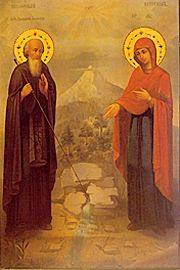
\includegraphics[width=.3\textwidth]{Athanasius_of_Athos.jpg}
\end{wrapfigure}

We've been given, as Christians, and have accepted, as fools, a very impoverished reading of Scripture, one in which Jesus emerges as someone so milquetoast\footnote{\url{http://en.wikipedia.org/wiki/Caspar\_Milquetoast}} that He wouldn't dare overturn the money-changing temples and bureaucratic stalls of Liberaldom or secular Democracy, could He by fickle mishap, arrive today. In a perverted sense, this is entirely true, for even this ``phase'' (degenerative as it may be), must exist entirely and utterly (though not \emph{self-consciously}) of His will, alone. As Cologero points out, this period of chaos must have Laws which govern it as well, just ones we're not as used to noticing. Yet, when the man comes around\footnote{\url{http://www.youtube.com/watch?v=k9IfHDi-2EA}}, the rules will get a lot less murky, quickly. There's a huge difference between God in heaven giving man time, and God descending to sort it out.

As for these difficult-to-discern-patterns of the Kali Yuga, could it be that part of the reason the Bourgeois Period is still alive and kicking is that ignorant men, latently of the brahminic or warrior caste, deliberately and desperately support it, seeing quite clearly the huge gap between the Third Estate epoch \& the epoch of the Shudra and the Outcast? After all, the merchant class is still ``objective'', at least; the Shudra is neither objective, nor free. Not seeing the huge gap between the Third Estate and that of their own (since it is unrealized), they volunteer to wage the struggle to stave off the tidal wave. This seems to be Mencius Moldbug's conclusion in this piece of punditry\footnote{\url{http://unqualified-reservations.blogspot.com/2013/06/civil-liberties-and-single-reactionary.html}}, for instance:

\begin{quotex}
Moreover, the fascist militarists who actually do this job are some of the best men in America. \textbf{American communism, for obvious reasons, loves to send America's best men to Afghanistan to get their private parts Osterized by fertilizer bombs}. This is American war since 1945: State solving the problem of how it can get DoD to stick its d--- in a blender. Solving it rather well, I'd say. Many of America's best men are in the Pentagon, and good men know how to obey, and into the blender goes that d---. Still, much testicle remains.
\end{quotex}


How long will the warrior caste (even more so those imitating it, either out of malice or virtue) be content with propping up a ``country'' designed to make life easy for the worst specimens of humanity? Now extending its obligation\footnote{\url{http://www.huffingtonpost.com/2013/06/28/obama-africa-hunger\_n\_3515684.html}} (and therefore, its power) to the entire planet? We shall see -- there are a lot of soldiers returning from the Middle East.

Also, it seems clear to me that the Spirit behind modern culture, for obvious reasons, wants to convince those who are formally, latently, or partially (if not truly) Good that Good and Evil are illusions, and that in the name of some catch-phrases like Equality \& Tolerance, Life ought to be made easier for everyone, even those who really aren't aware of anything above them, even their conscience. Isn't this what Evil would say to Good? That in reality, the distance between us is an Illusion? Something Jesus said comes to mind:

\begin{quotex}
And the lord commended the unjust steward, because he had done wisely: for the children of this world are in their generation wiser than the children of light. 
\flright{\textsc{Luke 16:8}}
\end{quotex}


Could it be that the Revolutionaries have long known (better than most) that seeing into the Nature of man is pre-requisite to changing things? Granted, they can only imagine that Good exists because of sluggish inertia, that it couldn't last, except as an inherited accretion and knee-jerk reflex (which of course, sees things backwards, given that most people engage in Evil for precisely this reason). But they have been adept\footnote{\url{http://en.wikipedia.org/wiki/Frantz\_Fanon}} at manipulating the remnants of the castes to achieve their end. Have you taken a literary criticism class, lately? All you read is literature of perversion and revolt. Take Sarah Kane\footnote{\url{http://en.wikipedia.org/wiki/Sarah\_Kane}}, for instance. Every effort is being made to extend the suffering of our ``elites'' through the ``middle'' and to unite that suffering with the lower castes. I saw a sign on a church recently which, against all odds, was actually apropos: ``While we play Church, God's creation becomes more corrupt.'' The Bible Belt itself is not as well off\footnote{\url{https://www.prbuzz.com/non-profit/70427-depression-and-pornography.html}} as it appears.

What would a Frankish noble have done if confronted with the modern world? Undoubtedly, after a tour through both prison and mental health facilities, he would have emerged much wiser and more cautious of General Law\footnote{\url{http://www.gornahoor.net/?tag=general-law}}. He would (in fact) lay plans with a prudence and cunning that would complement his innate qualities, and guarantee a larger success in the long run. On the other hand, the qualities he has innately, I lack. What can I learn from him, and where can I learn it? \emph{As noted above, there is the possibility of learning from our enemies, in that we see by negative example, how they employ means to ends and discern what is best for their kind}.

But there is much more for those who wish to transcend the purely Mephistophelean character of the clever Revolutionary, the spirit who negates\footnote{\url{http://www.pointandcircumference.com/macropoetics/Dante.htm}}, the composting bacteria which works among those whose souls die before they ever learned they had them:

\begin{quotex}
With Faust, the Romantic rebellion breaks out in full force. At the outset, the poem promises to take the reader ``from Heaven through the world to Hell.'' Note the inverse direction. And still less than Paradise Lost does Faust portray a coherent universe. A scene in a student hangout, a seduction drama, the spectacles of the first and second Walpurgisnacht, Faust's adventures as general, artist and civil-engineer-cum-dictator -- all this does not add up to a comprehensive portrayal of human life. The flames of Hell, briefly glimpsed, are taken about as seriously as in a comic strip; while Heaven (complete with a ``old guy'' Deity at whom the urbane and sophisticated devil thumbs his nose) is but the self-serving reflection of a middle world where the amoral have their way. \textbf{Unlike Dante's journey, Faust's is the opposite of instructive}. At the end the hero has destroyed the world and learned nothing, the angels confuse his ruthlessness with aspiration; and the author himself seems to have \emph{unlearned} whatever awareness of right and wrong he may have had at the outset. The final scene of {Faust} appears meant to contradict the scene at the summit of Purgatory where Beatrice insists on confronting Dante with his peccadilloes: ``A high law of G-d would be broken if Lethe were passed and such food tasted without some toll of remorse that sheds tears.'' Faust does not have to say he is sorry; enters heaven in the company of \emph{unborn children,} consciousness and conscience are effaced. The Israeli scholar Rivkah Schechter is, I believe, right in seeing Faust as the prelude to Auschwitz.
\end{quotex}


Hence, we turn to very particular texts, spiritual and literary and political, to nourish the awareness which we lack, which we horn-swoggled ourselves out of by accepting the Devil's food when we should have been vigilant.

\begin{quotex}
Law: mechanism which should be used in whatever way will generate the preferred result. Old fashioned law did too much to protect individuals from the social will. the mediocratic model avoids bourgeois notions such as principles or liberties. If the community believes someone should be punished, the legal system should not put obstacles in the way. The idea of providing protection for defendants from the state is no longer required, as modern state agents can be presumed to act on behalf of society rather than on behalf of an elite. \textbf{Mediocracy believes in having as many laws as possible, but enforcing them selectively. This provides maximum flexibility, since harassment can be targeted at appropriate individuals.} 
\flright{\textsc{Fabian Tassano}, \textit{Mediocracy}}
\end{quotex}


Christ the King told Satan to ``get thee behind me'' during the Temptation, which was the rough equivalent of a medieval king saying ``away with you, you varlet!''. Then, and only then, did angels minister to him. One of the traditional Christian's first tasks will be to learn not to accept a part in the inverted medieval passion play of the Spirit of the Age, but rather to wrestle with the powers and principalities (within himself, foremost) and force them to play the role in his own mystery play. For those ``waking up'', seemingly innocuous things take on spiritual significance. They ``manifest''. Do we wish to become cardboard characters, doomed to fire, in his play, or force him to step into our own?

Isn't this the root of the ``difficulty with Christianity''? Is it what it appears to be? It may look milquetoast, but this is an illusion. The regal-warrior spirit is carefully hidden in plain sight. Christ becomes a King by rejecting the world, the flesh, and the devil, by repulsing Satan's attempt to get him to play a part in a play in which his lines were penned by Satan. Isn't this what the Revolutionary narrative is all about? We may not know all, or even much, but we know \emph{enough}. Enough to begin to resist the temptation.

Spirituality such as found in the \emph{Philokalia} nourished the spiritual life of the Eastern Empire, \& from them, flowed westward, even if indirectly\footnote{\url{http://en.wikipedia.org/wiki/The\_Cloud\_of\_Unknowing}}. The Franks gladly submitted to the High King of Heaven: Chlodovechus exclaimed ``Oh, if I had been there with my Franks!''\footnote{\url{http://books.google.com/books?id=maMXAAAAYAAJ&pg=PA11&lpg=PA11&dq=had+I+been+there+with+my+franks&source=bl&ots=s2TTKEM_i4&sig=2KwFfrp1sd3jJHONKYTErse9aK4&hl=en&sa=X&ei=JFzMUfPuHcS1ygHmvIDABQ&ved=0CEUQ6AEwBA\#v=onepage&q=had\%20I\%20been\%20there\%20with\%20my\%20franks&f=false}}. It's possible to view this as an aberration and twisting of Aryan spirituality. But then, what do you do with such organizations as this\footnote{\url{http://en.wikipedia.org/wiki/Iron\_Guard}}? What about the Templars? Together, the Western tribes and the religion of Christianity created a fuller manifestation of Tradition (and corresponding higher aberrations, at times, when corrupt) than possible otherwise. \emph{Corruptio optima pessimi}.


Here is practical advice from the \emph{Philokalia} -- it has the smell of authenticity, as it isn't something one would ``make up'' on the spur of the moment. If one isn't a Brahmin, then simply gain the appropriate insight and apply it to your own circumstances. For instance, knowing that some thoughts have a demonic origin is highly useful, no matter what caste you belong to. I think you will see that this corpus of spiritual teaching is anything but ``sentimental'' and ``Semitic''. It is, in fact, triumphant and almost Promethean.

\begin{quotationx}
Similarly, anger, whether reasonable or unreasonable, obstructs our spiritual vision. Our incensive power can be used in a way that is according to nature only when turned against our own impassioned or self-indulgent thoughts. We must not therefore expend all our effort in bodily fasting; we must also give attention to our thoughts and to spiritual meditation, since otherwise we will not be able to advance to the heights of true purity and chastity.

If a man, still enmeshed in sin and anger, dares shamelessly to reach out for knowledge of divine things, or even to embark upon immaterial prayer, he deserves the rebuke given by the Apostle; for it is dangerous for him to pray with head bare and uncovered. Such a soul, he says, ought to `have a veil on her head because of the angels' (cf I Cor. 11:5-7), and to be clothed in due reverence and humility.

Blessed is the monk who regards every man as God after God.

There are times when the demons suggest thoughts to you and then urge you to rebut them with prayer; whereupon they withdraw of their own accord, so as to deceive you into imagining that you have begun to overcome such thoughts and to rout the demons.

You should be aware of this trick: at times the demons split into two groups; and when you call for help against one group, the other will come in the guise of angels and drive away the first, so that you are deceived into believing that they are truly angels.

When the intellect attains prayer that is pure and free from passion, the demons attack no longer with sinister thoughts but with thoughts of what is good. For they suggest to it an illusion of God's glory in a form pleasing to the senses, so as to make it think that it has realized the final aim of prayer. A man who possesses spiritual knowledge has said that this illusion results from the passion of self-esteem and from the demon's touch upon a certain area of the brain.

Know that the holy angels encourage us to pray and stand beside us, rejoicing and praying for us (cf Tobit 12:12). Therefore, if we are negligent and admit thoughts from the enemy, we greatly provoke the angels. For while they struggle hard on our behalf we do not even take the trouble to pray to God for ourselves, but we despise their services to us, and, abandoning their Lord and God, we consort with unclean demons.

One who has attained dispassion has not necessarily achieved pure prayer. For he may still be occupied with thoughts which, though dispassionate, distract him and keep him far from God.

Undistracted prayer is the highest intellection of the intellect.

The warfare between us and the demons is waged solely on account of spiritual prayer; for prayer is extremely hateful and offensive to them, whereas it leads us to salvation and peace.

When the intellect has been perfected, it unites wholly with God and is illumined by divine light, and the most hidden mysteries are revealed to it. Then it truly learns where wisdom and power lie... While it is still fighting against the passions it cannot as yet enjoy these things... But once the battle is over and it is found worthy of spiritual gifts, then it becomes wholly luminous, powerfully energized by grace and rooted in the contemplation of spiritual realities. A person in whom this happens is not attached to the things of this world but has passed from death to life.
\end{quotationx}


Ironically, there is a ``martial'' quality about the \emph{Philokalia}, which is consonant with the ``marching character'' of Christianity, itself a religion (in many ways) that was military. The Church, after all, was ``militant''. If it was\footnote{\url{http://riversfromeden.wordpress.com/2012/04/20/christians-in-the-roman-army-countering-the-pacifist-narrative/}} (perhaps dubitably) a religion of the lower castes, nevertheless, it should be remembered that it was through the Roman army \& Constantine, ultimately, that the religion won its victory over those, like Julian the Apostate, who wished to endorse Iamblichus and the NeoPlatonists rather than a religion. Christianity ``chose sides'' because it has a martial quality. I think this is the way to ``resolve'' the debate with neo-pagans: the Vedantic wing of Christianity wasn't strong enough to preclude an all-out war against all ``paganism'', so perhaps this should be rectified.

Yet Christ is a King, not merely a high priest. And the King is not mocked; He is no sentimentalist, but like a detached general, he awaits the inevitable outcome of His warfare. The King is Dead. Long live the King. The King is Coming. Life itself, the King.

\begin{quotex}
We believe that we invent symbols. The truth is that they invent us; we are their creatures, shaped by their hard, defining edges. When soldiers take their oath they are given a coin, an asimi stamped with the profile of the Autarch. Their acceptance of that coin is their acceptance of the special duties and burdens of military life---they are soldiers from that moment, though they may know nothing of the management of arms. I did not know that then, but it is a profound mistake to believe that we must know of such things to be influenced by them, and in fact to believe so is to believe in the most debased and superstitious kind of magic. The would-be sorcerer alone has faith in the efficacy of pure knowledge; rational people know that things act of themselves or not at all.

\flright{\textsc{Gene Wolfe}\footnote{\url{http://www.goodreads.com/author/show/23069.Gene\_Wolfe}}, \emph{Shadow and Claw}\footnote{\url{http://www.goodreads.com/work/quotes/40575}}}
\end{quotex}


The ``Third Wave'' of Christianity will come when Christians themselves reclaim their monarchic legacy, hidden in Scripture, of Christ as the prophet, priest, and king (warrior). If we apply the insights of the Philokalia quoted above, we would conclude that the history of the West has been a very careful, selective seducement of a predominantly warrior-religion, designed to ``set it up'' for a final illusion. That is, the glories of the Renaissance and the wonders of Science and the blessed peace of secular humanism are analogous to demonically-induced spiritual states designed to convince the one who undergoes them that they are ``favored'' and have reached ``deliverance''. However, there is still a chance that the victory of Logos in the West can be redeemed. That is, instead of the Divine withdrawing back into the Divine, the human can be drawn up into God (the aim of Christian warfare, which approaches the passions with warfare in an attempt to ``possess'' them for God). This can only happen if the West uses discernment to see that the Logos presented to it, of which it is most acutely aware, is to be sanctified to God \& taken up.

Thus, Western Christians have to see, at one and the same time, both the limitations of its Tradition (a warrior-religion) and the timelessness of it (a true reflection of something Transcendent, which was worth defending, albeit with more wisdom). This will involve restoring the ``Vedantic wing'' of the Faith, which will include esoteric studies. All resurgencies, ill-fated or blessed, of Christianity have begun with the return to ``Christ the King''.


\flrightit{Posted on 2013-07-05 by Logres}

\begin{center}* * *\end{center}

\begin{footnotesize}
\begin{sffamily}
\texttt{michel on 2013-07-06 at 10:39 said:}

Yes! If only more elites were like you Logres, then the restoration greatly longed for might stand a chance. I pray that the vigor of your writing is reflected in your actions.

\hfill

\texttt{Jason-Adam on 2013-07-06 at 12:26 said:}

This is amazing. I am inwardly in a similar state of being as Logres; independently I had come to the same conclusion myself that true, mediaeval Christianity was and is a militant, intolerant, warrior religion that gives to the man who follows it a high will to power and dominance, the ability to control his emotions, and a sense of community that gives the fight of our life meaning and purpose that transcends not only ourselves but all time and space... ... ... ... .

\hfill

\texttt{Logres on 2013-07-06 at 22:14 said:}

Thank you both for reading, although I am not one of the current elites (for which I begin to be more thankful, the more I learn). I wrote this partly because several readers last year had asked ``what to do?'', wondering if Christianity had anything to offer. I think, after reading in the Philokalia, that it does, \& have been pointed back to the theme of invisible warfare. Who would this NOT help? I am also glad that others perceive this too -- which makes neo-pagan denial of Medieval tradition all the more... well, odd. Thank you for your prayers, Michael.

\hfill

\texttt{Jason-Adam on 2013-07-08 at 12:56 said:}

Dear Logres,

may I ask do you have a personal regimen of spiritual practice ? I apologise if this sounds rude but as I see that we are similar minds though you seem to be of a higher level of development, I ask because I'd like to learn from you.

Also, have you read this book before ? It's Orthodox and ant-Catholic so I have some issues with it but all in all it makes a good defence of monarchy and the mediaeval Christian Tradition.

\url{http://www.romanitas.ru/eng/THE\%20MYSTERY\%20OF\%20CHRISTIAN\%20POWER.htm}


Lastly, in the past you've discussed Franz Bardon, would you recommend his books and exercises for someone looking for a transcendent experience ?

\hfill

\texttt{Logres on 2013-07-10 at 11:38 said:}

Jason, I think ``intolerant'' here is certainly in the sense of the modern word. That is, Christianity has no room for any competing -isms, heresies, etc., and maintains a traditional character, period. It is not interested in accomodating anything at the cost of its principles, although it may stoop in charity, infinitely. And it would certainly resist (if it were strong) incursions from foreign bodies who were designing to feed off its corpse (eg., modern Islam, the full blown Reformation political movement, etc.).

\hfill

\end{sffamily}
\end{footnotesize}


\section{Never the Twain Shall Meet}

I chose to write on \emph{The Dark Cloud of Unknowing} to illustrate something that is true that has been discussed here (that East \& West are not divergent in Tradition). The author was an anonymous Englishman during the 14th century; ergo, a quintessential ``Western'' mystic on an isolated island in the West. It is unknown who he was, but it is thought he was in the East Midlands (based on his language). He came after Richard Rolle, and before Walter Hinton, and is roughly contingent with Julian of Norwich. On the Continent, during this time of the Hundred Years War \& plague, the great German mystics also appeared. Europe was stirring with heresy, and the Reformation was not far off.

Romanides and Athanasios Bailey (whose Orla.Pubs is off the web now) maintain that the West lost the concept of ``energetic'' salvation; that is, the West favored a juridical model in which God ``reckoned'' righteousness or (prior to the Reformation) ``declared'' or ``atoned'' man into righteousness. This is the ``ransom'' theory that developed from Anselm\footnote{\url{https://en.wikipedia.org/wiki/Anselm\_of\_Canterbury}}. While we agree that certainly the deviations of Truth in the West have taken the form described by Romanides, we do not concur that the essence of Western Tradition is accurately described: the trend, perhaps, but not the essence or remnant (and there is always a remnant, Romanides should know this).

Specifically, the Frankish and Norman conquests of the West (followed by wars of conquest aimed at the Eastern Empire) are supposed to have caused the entire and widespread loss of genuine Christian understanding (and, given Eastern theology's emphasis on right wisdom of God and categories of thought, any resultant vital Christianity). However, as we shall see, Western communions made use of negative theology, and were aware of the same dogmas which governed Eastern apophaticism, however much it may be granted that it received less emphasis the farther West one went. As one author points out, the more \emph{cataphatic}\footnote{\url{http://en.wikipedia.org/wiki/Cataphatic\_theology}} Western theology has (as a safeguard against God-in-man's-image) the idea that the Logos is the archetype of man's Image. As an aside, I will note that the Eastern Church considers the 12th or 13th centuries an era in which sensual pleasure and softness enter the Western spirituality; the reply to this would be to note that while this is true, undoubtedly, it also came as part of the Troubadour movement, and could be viewed more positively (as Cologero has suggested) as a particular emphasis on Logos, peculiar to the West.

Additonally, John Scotus Erigena\footnote{\url{https://en.wikipedia.org/wiki/Johannes\_Scotus\_Eriugena}} had translated Dionysius from Greek into Latin much, much earlier in the Isles, so the English had access to negative theology, which influenced the author of the \emph{Dark Cloud}, and bore fruit in his treatise. It should be unnecessary to point out that the age of Cathedral building was founded on Dionysian theology, and had already taken shape\footnote{\url{http://en.wikipedia.org/wiki/Abbot\_Suger}}.

\begin{quotationx}
No one can think of God. Therefore it is my wish to leave everything that I can think of and choose for my love the thing that I cannot think. For while God may be loved but not thought. God can be taken and held by love but not by thought. Therefore though it is good at times to think of the kindness and worthiness of God in particular, and though this is a light and a part of contemplation, nevertheless, in this exercise, it must be cast down and covered over with a cloud of forgetting. You are to step above it stalwartly but lovingly, with a devout, pleasing, stirring of love and desire to pierce that darkness above you. You are to smite upon the thick cloud of unknowing with a sharp dart of longing love and do not cease no matter what happens. 6:130-131.

This, ``For the love of Jesus is very well said.'' For in the love of Jesus there is your help. Love is so powerful that it makes everything one (common). Therefore love Jesus and everything that he has is yours. By his godhead he is the maker and giver of time. By his humanity he is the very keeper of time. And by his Godhead and humanity together he is the truest guide of the choice and use of time. Knit yourself then to him by love and by faith. And by virtue of that knot you shall be a familiar partner with him and with all who are so knitted to him by love... 4:366-373. The example of all this is shown in the life of Christ. PC23:24.170 Mary models the way of contemplative prayer. So she hung her love and her longing desire in this cloud of unknowing, and learned to love what she could not see clearly in this life by the light of understanding in her reason, nor truly feel in the sweetness of love in her affection; so much so that she paid little attention to whether she had been a sinner or not. Yes! And so often I think that she was so deeply affected in the love of the Godhead that she scarcely noticed the beauty of his precious and blessed body as he sat so handsomely speaking and teaching before her. It seems from the gospel that she was oblivious to anything else either bodily or spiritual. XVI: 834-842
\end{quotationx}


The author makes the same energy/essence distinction that the Eastern Church makes: we never become God by nature, but only by grace.

Rather than ``the Jesus prayer'', we instead have this:

\begin{quotex}
Schort preier peersith heven.
\end{quotex}


(This, by the way, would even find an echo in the Puritan theology of ``Heaven Taken by Storm''). The use of one syllable words like ``God'' or ``Love'' are recommended for unceasing prayer, which builds on confession and regular meditation on revealed mysteries.

It is preferable to meditate on God's goodness, rather than one's own sin (contra-Calvinism), since whatever one thinks about ``sits between'' God \& the self, although he does not deny that exoteric or ordinary religious meditation lays a foundation from which to build true contemplation, by God's grace, later on, which is given regardless of merit or dis-merit, but according to desire.

\begin{quotex}
Thinking may not goodly be getyn withoutyn reding or heryng comyng before... Ne preier may not goodly be getyn in bigynners and profiters withoutyn thinkyng comyng bifore.
\end{quotex}


How will they believe, if they have not heard? He suggests that many are against contemplation, and have a false humility (thinking that their piety is perfected as high as may go in exoteric meditation) \emph{because they are simply unaware of any higher path (they have not heard, and are deceived in imagination)}. So this is a defense of the esoteric or contemplative way, but he preserves their unity by arguing that the higher active path \& the lower contemplative path are actually the same path. Additionally, he links these three paths with the ``beginner'', ``proficient'', \& ``perfect'' which we see used by Garrigou-Lagrange\footnote{\url{https://en.wikipedia.org/wiki/Reginald\_Garrigou-Lagrange}} in his small work on Christian conversions.

I will also note some affinity in this work with later Western development in Pierre-Caussade's Sacrament of the Present Moment\footnote{\url{https://en.wikipedia.org/wiki/Jean\_Pierre\_de\_Caussade}}. I believe that one could take Western manuals such as these (while recognizing legitimate shortcomings and criticism) and build an impressive library of religious contemplation that would bear and stand comparison with modern day Eastern modes or models.

The point is not to say ``nu-uh, we have it too'' but rather encourage Western readers to look deeper into their own tradition -- not without reason is it said (not to our honor) that prophets are not without honor, except in their own country. But why go so far East? Surely there are far spiritual and physical countries at hand, who have more elective affinities with our background, that remain, yet, Christian?

The author of \emph{The Cloud} advocates two interesting strategies for overcoming mental ``thoughts'' and entering into love. Firstly, one can ``look over the shoulders'' of the daily thoughts which crowd you, focusing on something beyond them, while not obliterating them directly. Secondly, one can ``cower down to them and surrender to them''. This last strategy is particularly recommended by him as a means of annihilating the enemies, for God will swiftly come to the rescue of His children who lie helpless before a wild boar. Additionally, this keeps the Ego from getting involved in combat, which only ``messes things up'' (according to this mystical author).

He is not advocating Quietism\footnote{\url{https://en.wikipedia.org/wiki/Quietism\_\%28Christian\_philosophy\%29}} (since one continues outward religious observance) but, rather, the attention to thoughts: observing their arrival with discretion and judgement, a practice that is fundamental, say the Fathers of the \emph{Philokalia}. One surrenders to the interior work of God, while exercising patience and obedience outwardly. Again, we see that Christianity is in this sense, martial, since the soldier maintains discipline in a fight which is not necessarily (even by esoteric standards) appearing to go well. Hope is instead placed in the action of Grace, rather than merely the enhancement of Nature. This is the Christian legacy, both inwardly and outwardly.

The author also translated \emph{Dionysius' Divinitie Hid}, \& wrote several other treatises, which quote Augustine, Aquinas, Aristotle, and Richard St. Victor (placing him within the European stream). Those who will pursue God through ``un-thinking'' Love will end up grasping many intellectual mysteries along the way, and the Love we have is passive only towards God : it actively overcomes discursive thought (placing all creatures whatsoever in a ``cloud'' of forgetting) and is naked only towards God, being active in the sense that it moves instinctively back to the source of all Being, God who exists by Nature in the state we must attain through Grace alone.

The same attention to thoughts that is recommended in other Traditions is found here, embedded within the Christian tradition.

\begin{quotex}
... If a man happened to be your deadly enemy and you heard him cry out with such terror, in the fulness of his spirit, this little word ``fire!'' or this word ``out!'' you would have no thought for his enmity, but out of the heartfelt compassion, stirred up and excited by the pain expressed in that cry, you would get out of bed even on a night in mid-winter, to help him put out the fire, or to bring him comfort in his distress. O Lord, if a man can be moved by grace to such mercy and compassion for his enemy, his enmity notwithstanding, what compassion and what mercy will God have for the spiritual cry of the soul welling up and issuing forth from the height and the depth, the length and the breadth of his spirit, which contains by nature all that a man has by grace, and much more!
\end{quotex}



\flrightit{Posted on 2013-07-12 by Logres}

\begin{center}* * *\end{center}

\begin{footnotesize}
\begin{sffamily}
\texttt{Jason-Adam on 2013-07-13 at 12:04 said:}

Your posts are always full of meat, Logres. I commend you.

\hfill

\texttt{Jacob on 2013-07-13 at 23:55 said:}

Great post as always.

I find it interesting that you would mention a text written by a Jesuit. The Jesuits sometimes use language that at least to me seems similar to some non-dualist authors. Guenon mentioned once in one of his books (can't recall which) that the spiritual exercises were similar to techniques used by esotericist, but lead to completely different results. Is that something inherent in the spiritual exercises, or is Ignatian spirituality a great way in the Western tradition to reach our goal? It certainly has a somewhat martial nature.

From what I understand at from reading Internet articles, the jesuits are somewhat overrun with Fruedian psycho-babble and other non-traditional ideas, but people like Hans ur Von Ballthasar was a big supporter of Tomberg's Meditations (or at least wrote a foreword to it). What do you think?

Sorry if this question has come up before or if I have misunderstood something.

\hfill

\texttt{Logres on 2013-07-14 at 10:06 said:}

Jason, thanks for the feedback: it's good to know my intention to give a lot of material in the essays comes through without cluttering it up.

Jacob: I am not qualified to answer this, as the text mentioned is the only portion of Ignatian spirituality I have read; Cologero is likely to know more, although I will attempt to do some research (perhaps the next article?). I do not see, however, how any objection could be raised to Caussade's work, judging its spirit, unless it were a very subtle one I am missing.

\hfill

\texttt{Jacob on 2013-07-14 at 13:43 said:}

Ok, thanks Logres. I'm sure Cologero will stop by to elaborate, and thanks again for another post.

\hfill

\texttt{Logres on 2013-07-14 at 22:00 said:}

I hope Cologero comments (or someone else who is better read than I) on Jacob's excellent question. I've read part of Loyola's Life, and it seems to be that of someone who experienced the divine in an ascetic way, so I am anxious to find out more of what Guenon's judgement was on the subject. All of my posts are aimed at framing Christian theology in a broader context which parallels traditional metaphysics, although obviously as a Christian (albeit someone who came from a Reformed background) I believe that Christ as a ``true myth'' and the ``avatar of avatars''.

\hfill

\texttt{Cologero on 2013-07-15 at 00:20 said:}

Jacob, that book you referred to is Perspectives on Initiation, in which he claims that the spiritual exercises were partially inspired by initiatic methods of Islamic origin, but for a different end. They follow the Western path of purgation, illumination, and union. I don't know if or where Guenon describes the Islamic techniques and what their goals are, presumably ``deliverance'' which must be beyond union. On the plus side, at least from Guenon's point of view, Ignatius was not a ``mystic'' (in Guenon's use of the word) since his exercises are active, not passive.

The Jesuits have certainly deteriorated since their founding; the question is how did their strict formation, spiritual exercises, and dedication to learning not protect them. I think anyone wanting to start on order on that model, and it is a good one, needs to look into that.

Balthasar left the Jesuit order long before his introduction to MoTT.

\hfill

\texttt{Jacob on 2013-07-15 at 01:27 said:}

Ok thanks Cologero.

That is a very good question on their degeneration. I'll certainly think on it. But do all traditions not naturally degenerate because the quality of the person does the further we sink into the KY? Or is it more willfully on our part than that?

Of course the current pope is a Jesuit, but I personally am not sure what to think of him as a person. He has spoken out against capitalism a lot which I hope he does, because he sees the worthlessness of materialism like Evola; and not because he is a pandering to leftist.

\hfill

\texttt{Logres on 2013-07-15 at 12:09 said:}

I need to look into Guenon's definition of mysticism, but the author of this treatise insists that the ``passiveness'' we have before God is active in a sense: a body has legs and can walk, although it cannot see, it can feel and walk. This is the analogy he uses, but does insist on a prior foundation of confession, rites and rituals, and also contemplation. This would safeguard (certainly in a better era) the Intellect.

\hfill

\texttt{Jason-Adam on 2013-07-15 at 21:29 said:}

All things decay and die, only God is immune from this, so dont blame Jesuit spirituality for the failure of the order in our times.

Cologero, who would you say is a mystic in the Guenonian definition ?

\hfill

\texttt{V.O. on 2013-07-17 at 05:55 said:}

``the author of this treatise insists that the ``passiveness'' we have before God is active in a sense''

The claimed passivism of the mystical often informs Evola's critique of Christianity, but this is incoherent from an Orthodox perspective.

Losski writes:

``The doctrine of the energies, ineffably distinct from the essence, is the dogmatic basis of the real character of all mystical experience.''

The energies of God are equivalent to the revelation of God to the world; as conditioned by the energies, mystical experience is thus the contemplation of this revelation.

What could be more ``active'' than the dedication to the revelation that shatters the pretense of the entire world?

\hfill

\texttt{Cologero on 2013-07-24 at 05:57 said:}

J-A, probably Therese de Lisieux is a popular example of a mystic in the Guenonian sense.


\hfill

\end{sffamily}
\end{footnotesize}


\section{Restoration, Revival, Renaissance}

\begin{wrapfigure}{rt}{.3\textwidth}
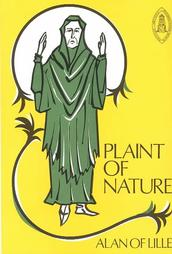
\includegraphics[width=.3\textwidth]{plaint-nature-alain-de-lille-paperback-cover-art.jpg}
\end{wrapfigure}

The order of these nouns is deliberate. Secular humanists desire to have the last without either of the first two, particularly and most insistently, the first. Christians are generally unconcerned or even aware of the first, \& if it is brought to their attention, they become truculent. The third also escapes the notice of many of them, who have been relegated to the merchant or warrior castes, or who have been converted while being laborers or even \emph{shudras}. In fact, one of the primary dogmas of this era is the idea (variously expressed) that ``you can't go back'', that ``(all) change is good'', \& that ``new is always better'', and almost no one dissents from it. (Wendell Berry hilariously points out\footnote{\url{http://www.jesusradicals.com/wp-content/uploads/computer.pdf}} that if using a computer is a new idea, then not using one is an even ``more novel'' one.)

\textbf{\emph{That is why it is important to pursue one's vocation and caste, as well as practice the ``lesser mysteries}}``, rather than spend too much time worrying if one has attained supreme Enlightenment. Because in the New Age worldview, to not have reached the summit of Mount Parnassus is to not have done anything. This reminds one of A. Jarry's evil motto -- ``\emph{Until we've destroyed everything, we haven't done anything}``. This bastard-like, ungrateful, and rebellious attitude has transferred itself out of the failed 60's movements, \& into the ``mainstream''. Nowadays, if someone doesn't have visions of the angels, adopt children from foreign countries, and float through life in a haze of super-tolerance and up-to-date information, then why possibly bother? Beware of thinking like those who are masterless and rebellious.

Tracy Lee Simmons points out in \emph{Climbing Mount Parnassus}\footnote{\url{http://www.amazon.com/Climbing-Parnassus-Apologia-Greek-Latin/dp/1933859504}} that

\begin{quotex}
The foundations of the modern world are viewed more competently from this (the ``classics'': study of Greek/Roman civilization) height. Poetry, drama, democracy, idealism, scientific curiosity, and so much else furnishing our minds are better grasped, and better judged. We drift without classics, floating on our own deracinated, exiguous islands. And we become fodder for demagogues. We need not a revolution, but a restoration.
\end{quotex}


I will give you an example. Alcibiades, in Thucydides' \emph{History}, defines democracy as the concern simply that the good of all be given due consideration, rather than merely the good of a few (the non-slaves). Now Alcibiades was bargaining for his life with the Spartans, to whom he had fled in exile, so perhaps he was being disingenuous. Nevertheless, even the villains and knaves of ancient history have an unpolished grace that should make us blush. Jose Maria Gironella in \emph{The Cypresses Believe in God}, has Ignatio say that he defines socialism as the belief that the ``rich shouldn't have everything, and the poor nothing''. Rather than hate democracy uncategorically, perhaps it would be better to examine it \& to see where it legitimately applies (eg., local self-governance) \& where it becomes an ersatz religion, a demon, and a false God.

In the context of real Restoration, of that which is always True \& is always so \& abides forever, a great many false dichotomies and catch phrases dissolve into clarity. GK Chesterton, for instance, attempts in his Agrarian and Distributionist thought (which he bases on Hillaire Belloc and other Catholic thinkers), to demonstrate what ``Christian democracy'' actually meant, rather than what it came to mean detached from God, the soil, and all wisdom.

Therefore, the first thing or first question is ``what constitutes Restoration''? As Jacques Barzun notes of education, it is dangerous to look too closely at the object (like staring at the sun, or trying to see the Pleiades head on), because the growth of ``education'' (or Restoration) is a slow, intangible, and subtle process which is difficult to assess. It might be better, argues Barzun, to stick to teaching Latin, Greek, chemistry, and the rest of the traditional subjects well (just a few of them), and let ``education'' occur like the growth of a tree. So, work at the destined work of your vocation; practice what lesser mysteries Providence brings to your attention; \& assiduously and patiently cultivate your spiritual garden. You are climbing Mount Parnassus\footnote{\url{http://en.wikipedia.org/wiki/Mount\_Parnassus}}.

If one is drinking from the fountain of Tradition (which can be increasingly recognized the more and deeper draughts one imbibes), then you need not fear to lose the way. Alain de Lille (doctor universalis, d. 1203) wrote of the ``intelligible sphere whose center is everywhere, and whose circumference is nowhere'' because he had drunk from it. And where did he find such wisdom? Of course, first of all, he had read or been told of such a hermetic tradition. Yet also, it is said that he was preparing a lecture on the attributes of God, and had gone down to the Seine River bank to walk. He met a young child, who had dug a hole in the sand. The teacher told the boy he was lecturing on God tomorrow, and asked what he was doing. The child said, ``I am putting the river inside of this hole''. The doctor laughed heartily, and said there was no possibility of that, that his purpose would fail. The boy looked at him, and said that it would be equally impossible to speak of God the next morning. Alanus\footnote{\url{http://www.princeton.edu/\~achaney/tmve/wiki100k/docs/Alain\_de\_Lille.html}} was shattered, and although he showed up the next morning, he tore his robe off, \& without another word, strode out of the university to join a monastery and find the answer to the riddle. God will speak to you in homely terms, in the lesser mysteries, in exoteric religion or philosophy, as surely as in the greatest terms, \& the Christians assert that this is due to the Incarnation.

Incidentally, for Christian readers, I will recommend Coleston Brown's \emph{Magical Christianity}\footnote{\url{http://www.amazon.com/Magical-Christianity-Symbols-Spiritual-Meditations/dp/0835608557}} (the source of the Alanus de Lille story) as a sourcebook for uncovering the Tradition hidden within their own religion. It matches well with Iamblichus' progression of the first ten numbers, and we shall see if it has any correspondence with the zodiac of Hercule's labors, as well.


\flrightit{Posted on 2013-11-23 by Logres}


\section{Western Social Order}

\paragraph{Part I} Cologero points out that quibbling over minor points of philosophy \& actualizing states of being are not equivalent for the noble character. That is, philosophical debate is not for the gentleman, beyond a certain point. Surely the West (as such) was built upon such a a fundamental impulse, as the aristocracy of the Franks and Germans were a rough and ready group of fighters, with little taste for Byzantine theology. John Romanides\footnote{\url{http://www.romanity.org/htm/rom.03.en.franks_romans_feudalism_and_doctrine.01.htm}} has criticized this substantially, but does not address in any way the fact that the West managed to not merely retain much more than a shadow of Byzantine mysticism, but actually to incorporate and seemingly ``add'' elements of Tradition with which the East was less familiar. Cologero has discussed this under the title of The Three Orders\footnote{\url{http://www.gornahoor.net/?p=5198}}. Byzantium retained the purity of dogma from Constantine's day, but the social order was collapsing. They were apparently unable to escape the curse of political factions: in other words, they lacked unity\footnote{\url{http://en.wikipedia.org/wiki/Byzantine_Greeks}}. Procopius\footnote{\url{http://en.wikipedia.org/wiki/Procopius}} even relates a story about Justinian the emperor which is intriguing;

\begin{quotex}
And some of those who have been with Justinian at the palace late at night, men who were pure of spirit, have thought they saw a strange demoniac form taking his place. One man said that the Emperor suddenly rose from his throne and walked about, and indeed he was never wont to remain sitting for long, and immediately Justinian's head vanished, while the rest of his body seemed to ebb and flow; whereat the beholder stood aghast and fearful, wondering if his eyes were deceiving him. But presently he perceived the vanished head filling out and joining the body again as strangely as it had left it
\end{quotex}


... perhaps some of the ``pure in spirit'' who could perceive his disappearing head were Pythagoreans. In any case, political factions dismembered Byzantium long before the Seljuk Turks and the Crusaders delivered the finishing blows. Although I don't agree with the pejorative, the adjective ``Byzantium'' today still describes a certain kind of stifling, convoluted atmosphere that is almost impossible to fathom. In fact, Cologero has also pointed out that the East/West schism was primarily exoteric, \& should not (in fact) be recognized as decisive or definitive by those who have eyes to see. Just as the Inquisition's attack on esoteric bodies within the Church should be ``ignored'', in the sense of recognizing it as a natural kind of failing in these situations, while retaining both facets for future use, the West vs. East problem is also illusory, if one is trying to deduce eternal principles out of historical dialectic. Instead, move from Unity towards the One, rather than reasoning from the many back to Unity.

The Revolution is derived from such dialectic; although Romanides is not a revolutionary, his theology has made it in some senses more difficult to rapproche with West, in that there is nothing constructive or creative about it, and one has to ``supply'' what is missing. Indeed, had it not been for Gornahoor, I myself would have found his logic convincing, and would no doubt by now be reading Alexander Dugin and plotting to immigrate to Russia, or at least pining for it. A Revolutionary reasons thusly:

1. The Church has done bad things, or been implicated in the doing of said bad things.

2. Therefore, we are better off today with the Church in chains, culturally, if not annihilated forever.

Therefore, the upshot today is that, ``as for my people, women are their oppressors, and children rule over them''. Isaiah 3:12.

As Robert Nisbet has pointed out in \emph{Twilight of Authority}\footnote{\url{http://www.amazon.com/Twilight-Authority-Robert-Nisbet/dp/0865972125}}, the modern liberal state that has resulted from the above reasoning (which is shared by some of the brightest and best young people I have met or been acquainted with) drifts toward either chaos or a monolith that reduces individuals to atoms, with no power or defense against the centralized state, which has been optimized (ostensibly) for the good of all, and particularly the new ``individual'' neo-bourgeois\footnote{\url{http://www.firstthings.com/web-exclusives/2012/08/the-neo-bourgeois-project}}. Phillip Rieff is a Jew\footnote{\url{http://en.wikipedia.org/wiki/Philip_Rieff}} that every man of Tradition ought to read: his book on \emph{Teaching \& The Second Death} closed off, forever for me, the idea that the new ``individual'' had anything to add -- his diagnosis of the spiritual sickness that grips us is profound. It is no use arguing, you have to treat the condition as an illness; in this Romanides and Tomberg are in essential agreement, as are all the Traditional thinkers.

Unfortunately, a lot of the young are ineluctably drawn to the syllogism above, and those of old age, who are hopelessly lazy and self-corrupt, encourage them. What the enthymeme\footnote{\url{http://en.wikipedia.org/wiki/Enthymeme}} above leaves out is significant. What, for example, happens to other Ideals besides the Church that become tarnished? Are they to be discarded as well? And what happens when Man has tarnished his last Ideal? Should Ideals themselves be given up? What would that look like? Can Ideals be rehabilitated? Why should the abuse of an Ideal disavow the goodness or reality of that Ideal? Are Ideals inevitable, even when denied? Why did the Ideals fail to begin with? Are they inherently evil, inviting abuse? Why should this be? Can Ideals be critiqued by anything else other than Ideals? Were the Ideals ever properly instituted in the first place? Why or why not? What would a false Ideal look like, and how would we recognize it?

Cologero rightly points out that Socratic dialogue can end in \emph{aporia}. But what if the Socratic dialogue was done, as he suggests, within a framework of actualization, as acts achieving states of being? That is the project of Gornahoor, or at least, the part I am most familiar with and best understand. It may be preaching to the choir, but it's certainly better than what you'll get at the average Sunday School, and you'll know something more than a four-part Gospel harmony, although such things have value.

As an aside of interest, an author that links to the site frequently, Brett Stevens, has written a popular piece\footnote{\url{http://www.amerika.org/politics/destroy-white-nationalism/}} which summarizes in popular form some of the cogent criticisms of political European nationalism that Cologero has made in much more in depth and subtle terms. Some of the readers may find the piece useful and convincing, as I did. It points us in the direction of achieving what our director and founder a scale of spiritual order, rather than appealing to the baser parts of human nature, our own and others.

The West, historically, has excelled at achieving difficult balances with periods of crisis, from its inception, which involved multitudes of groups and periods of disorder. It can be hoped that it will do so again.

\paragraph{Part II} A recent comment by John of Salisbury made me think:

\begin{quotex}
Not only were these scholars unable to drive out the bad scholars, but in combating insanity, they temporarily became insane...
\end{quotex}

I thought about this question in relation to other questions or comments relating to the ``inner struggle'' of the man of Tradition in today's very untraditional world. I had a good acquaintance on the Internet give up study in that area because he needed something more cheerful. If you will notice, Cologero does not restrict his reading to Guenon and Evola, but also studies a wider range of writers on a diverse array of subjects. It is probably true that a steady diet of Evola and Guenon has the potential to unsettle one. Caleb is planning to put up a post that addresses part of this, in that Tomberg's \emph{Meditations} are designed to lay a firm foundation, without which (if you neglect the first card of the Tarot), the rest becomes unstable. Cologero has done a fine job of supplementing Evola and Guenon (whom he terms the ``Master of Tradition''), with the meditations on the \emph{Meditation}. The Tarot discussion list (and Caleb's article) is designed to assist in this process. In trying to imitate our betters, we often overstep or over-estimate our own capabilities, sometimes not deliberately, as we try to ``come up to speed''. Incidentally, much of Phillip Rieff's thought in \emph{Culture and Its Second Death} explores the danger of being initiated into our elder's/better's debates too swiftly, including the fundamentally erotic desire to criticize those to whom we owe everything. Rosenstock-Huessy called this ``Teaching too Early, Learning to Late'', in which the danger is that we learn just enough to be dangerous, to ourselves and others.

\begin{quotex}
A little knowledge is a dangerous thing -- drink deep, or taste not the Pierian spring!
\end{quotex}


I can certainly relate to this, having passed in and through and back into such phases, over the course of my short 40 years. In the case of Gornahoor, the best possible foundation has been laid down, but it has been made freely and openly available (with no secrets) laying out the Arcanum that must be mastered before entrance into the Mysteries. But the danger is still there, just a necessary one: in our chaotic age, one has to invite everyone, since those who should be ready are not. Jesus gave this in parable form in the tale of the Wedding Feast invitations.

John of Salisbury cites a medieval authority who claimed that there are three types of souls: those who fly, those who crawl, those who walk. Those who fly learn much, and swiftly, but soon forget. They make poor students (I think this is my soul's danger, for instance). Poetry may be a help to such students. Those who crawl are dull of soul -- in Pythagorean circles, they would not be allowed to be initiated, for instance, during the old days. Those who walk, steadily and constantly, those who are pilgrims, make the best students, fit to climb Parnassus and drink from its springs.

There was another recent article on Gornahoor that explained some of this quite well -- different types or souls have to be handled\footnote{\url{http://www.gornahoor.net/?p=6980}} differently. Michel's comment on this post\footnote{\url{http://www.gornahoor.net/?p=7093}} by Cologero gets to an esoteric root that lies behind a lot of misunderstandings that occur during these confusing times. Different types or \emph{differing potentials} require completely different spiritual trajectories: in Mouravieff's words, if the center is God, and we all find ourselves scattered at various circumferences, the trajectory back of necessity takes a variety of angles and forms. And some people don't necessarily manage to make a straight line, either!

All of this is to say that the ``care of souls'' remains paramount: even if one is caring for one's own soul, in which case, even more ``care'' is required, not less.

\begin{quotex}
In some denominations of Christianity\footnote{\url{http://en.wikipedia.org/wiki/Christianity}}, the cure of souls (Latin\footnote{\url{http://en.wikipedia.org/wiki/Latin_language}}: \textbf{\emph{cura animarum}}), an archaic translation which is better rendered today as ``care of souls'' is the exercise by priests\footnote{\url{http://en.wikipedia.org/wiki/Priest}} of their office. This typically embraces instruction, by sermons\footnote{\url{http://en.wikipedia.org/wiki/Sermon}}, admonitions and administration of sacraments\footnote{\url{http://en.wikipedia.org/wiki/Sacrament}}, to the congregation\footnote{\url{http://en.wiktionary.org/wiki/congregation}} over which they have authority from the church\footnote{\url{http://en.wikipedia.org/wiki/Christian_Church}}. In countries where the Roman Catholic Church\footnote{\url{http://en.wikipedia.org/wiki/Roman_Catholic_Church}} acted as the national church, the ``cure'' was not only over a congregation or congregations, but over a district. The assignment of a priest to a district subdividing a diocese was a process begun in the 4th century AD. The term \emph{parish}\footnote{\url{http://en.wikipedia.org/wiki/Parish}} as applied to this district comes from the Greek word for district. Those who earned their living on a position without cure of souls were known to have a sinecure\footnote{\url{http://en.wikipedia.org/wiki/Sinecure}} (hence the expression).
\end{quotex}


Even when one is taking the ``dry path'', and investigating the layers of one's own soul in an esoteric manner, there is a care or ``art'' involved, \& note merely a science (this may be where the balance between East and West is reached, as the East approaches spiritual things almost mechanistically).

This pervasive feeling of hopelessness, of fighting against fearful odds, of being doomed, can be viewed and attacked from several angles. Since I've been asked several questions lately that pertain to it, I assume it's relevant, and am relating it back to the conquest or reconquest of Western Social Order. It may relate to the ``noonday demon'' that attacked the desert monks, a lassitude and despair that could only be overcome with productive work: this is why Cologero has emphasized that practicing one's caste and craft is as important as becoming ``enlightened''. This is in the spirit of the Patristic fathers, who had monks weave baskets, plant gardens, build buildings, etc., because (as the \emph{Philokalia} teaches) Satan can only attack along one front when we are working, rather than all fronts simultaneously.

First, as noted above, it is paramount to appreciate that simultaneously, Guenon is both the measuring rod (for several reasons, not least of which is that our teacher, Cologero, regards him as such) \& also that which is to be transcended. That is, the goal is to not make Guenon's mistakes. For a Westerner, then, we recognize that Guenon advocates a path away from exoteric form, in favor of an East that (in his day) was less tainted, and a source of hope. Of course, today, we see that the East has imitated the West, and that Coca-Cola and blue jeans have flattened the globe. Cologero has done a huge service in upholding Guenon's standards, but eschewing some of his conclusions.

Secondly, we avoid the pit of getting caught up in erotic disputations over nothings. We've seen a lot of posters come and go -- many wanted to dispute with Cologero over various bagatelles or supposed critical mistakes. The Hermetic method (favored by Western thought that is faithful to Plato, Bonaventura, etc.) eschews such disputes, as does St. Paul. Avoid fruitless disputation... .

Thirdly, for the above reasons, we should probably avoid a pure diet of Guenon and Evola and traditional thinkers, if for no other reason (this is an additional one) than that those who battle vampires and monsters develop a kind of hardness about them that can be monstrous. It is not natural (and they would have recognized this) to have to spend your whole life in combating insanity, from dusk till dawn. Rejoice over their gift to us, but don't forget to plant a fig tree. Our times are conditioned by different possibilities; many battles are lost, others are looming, and some new possibilities have deepened or awakened. As our master Goethe says, \emph{a man who is not of his own times, can be a man of no other time}. Read a mystery novel, watch a movie. Even the medieval thinkers (such as the author of \emph{Philobiblikon}) says that it is possible to appreciate modern thinkers and writers, along with the ancient ones. Evola and Guenon have modern dimensions to their thinking. \textbf{\emph{The entire Quantity/Quality distinction can become (at times) almost a quantitative category which taints our perception of Quality}}. The medievals emphasized the value of Estimation, in which the beginner practiced his craft of working by esteeming that which had objective, natural moral value, in their own day. Even in our day, there are people which have dignity, things or activities which have value, etc.

So temper it. If it gets you down so much you can't function at all, and quenches the inner fire, even down to the last spark, find something more cheerful for awhile. But realize it isn't Guenon or Evola's fault -- its a privation within ourselves. Luckily, within the Christian esoteric and exoteric tradition, we are allowed holy-days and feast days, in which we can re-create ourselves in the wonder of Creation, which abides, even in our horribly dark days. As our teacher Wordsworth says, \emph{one impulse from a vernal wood, can teach you more of man, of moral evil and of good, than all the sages can}. Presumably, Wordsworth didn't even have access to the sages which we do, so temper this with grateful knowledge, and spend some time learning the constellations, or admiring the wonder of a storm. In the \emph{Romance of the Rose}, an initiatic text, the writer asks rhetorically, what can be done with someone who doesn't appreciate the approach of Spring and the gods of Love!

Fourthly, there are other thinkers out there, perhaps secular ones, who can be as circumstantially valuable to us as Evola and Guenon, under certain conditions. I would class Phillip Rieff in this category, at least for those like myself. He gives a feeling of ``utter hopelessness'', but this is meant to be curative, in the spirit of Kafka\footnote{\url{http://books.google.com/books?id=45d6JsdVFaIC\&pg=PA50\&lpg=PA50\&dq=kafka+withered+hand\&source=bl\&ots=yOFVlpXRLO\&sig=VxXgUnJ-qHSfTDsw6og2NQcl8w8\&hl=en\&sa=X\&ei=PL0LU-bSK8XJsQT5vIG4BQ\&ved=0CGkQ6AEwCQ\#v=onepage\&q=kafka\%20withered\%20hand\&f=false}}. And it is aimed at the \emph{hubris} and ignorance of our modern self. Some self-hatred and the cutting off of limbs or eyes is appropriate (symbolically speaking) as most moderns are in a rather unique bind, being cut off from their own soul, which is
\emph{naturaliter anima Christiana} (Tertullian). So a little Theodore

Dalrymple, Richard Weaver, Phillip Rieff, Christopher Lasch, or other such notable secular saints is of great value to many -- if nothing else, it's a safer way to process (like the liver) the toxins of our intellectual age, which are in the air we breathe. Just realize that (being creatures) we have to balance our diet intellectually (until we are enlightened, when all things become pure). \emph{If you read Rieff, you'll realize you should probably be listening to Haydn's classical music (or some other classical composers!)}. However, the trip is worth it. Rieff shows us (in \emph{Culture, Its Second Death}) that all of our spiritual states (even the Sartrean hell, which lurks for us today) are manifestations of our soul's possibilities along the Vertical. There is no escape (or no false escape) from the vertical -- we have to face up to the real problems and questions, first. As Solomon says, the house of mourning is more fruitful than the house of laughter, if it is a mourning of repentance. If (however) one is past this, then one is past it.

Christians are ``ahead of the times'': we are not immersed in them. So just because this is the Kali Yuga, it (everything) still matters very much. One of my teachers, a Lithuanian who taught literature, once berated me for reading Christianity into Shalamov's\footnote{\url{http://en.wikipedia.org/wiki/Varlam_Shalamov}} work: the whole point of his story was how small acts had meaning in and of themselves, regardless of a Christian interpretation or outcome! The character (interned in a camp) had found a can of condensed milk. For a short time, this can was God's grace, without being officially God's grace! Such is the mighty, eternal, and infinite mercy of God, which mercy endures forever, His chief attribute. This is the lesson Tomberg teaches also -- not control, but mercy and Love, which is the Queen of Magic.

This is our burden, this is our time. It is hard, and we have to help each other. We have to show mercy, while remembering Truth. I hope this is encouraging, \& look forward to being taught and helped by others on this path.

\paragraph{Part III} In the \emph{Philobiblon\footnote{\url{http://www.philobiblon.com/philobiblon.shtml}}}, Richard de Bury (Bishop of Durham) justifies his love of books in a Christian framework by pointing out that Plato is said to have paid 10000 dinars for a rare scroll of Philolaus. Philolaus'\footnote{\url{http://en.wikipedia.org/wiki/Philolaus}} work was most likely a transmission of the teachings of Pythagoras, who had gone to Tyre and to Egypt in order to learn from the masters there. Plato used this work to compose the \emph{Timaeus}, one of the more ``mystical'' of his treatises. If you are wondering where the Eastern Church got its teaching on the total dissimilarity between the essence of God (unknowable) and His energies (especially those manifested in Creation), this is where it comes from: it was part of the Tradition embodied in Hellenic wisdom, culled from Egypt:

\begin{quotex}
This is the state of affairs about nature and harmony. The essence of things is eternal; it is a unique and divine nature, the knowledge of which does not belong to man. Still it would not be possible that any of the things that are, and are known by us, should arrive to our knowledge, if this essence was not the internal foundation of the principles of which the world was founded, that is, of the limiting and unlimited elements. Now since these principles are not mutually similar, neither of similar nature, it would be impossible that the order of the world should have been formed by them, \textbf{unless the harmony intervened} . . .
\flright{\textsc{Philolaus}, \emph{Fragment DK 44B 6a.}}
\end{quotex}

\emph{Out of Egypt}, said the Patristic Fathers, \emph{have I called my Son}. Here was an example of the higher, ``secret'' meaning of Scripture, which they discerned in the literal text, and defended in their apologetics. The \textbf{\emph{Logos}} (of course) is the intervening harmony which causes the co-inherence\footnote{\url{http://web.sbu.edu/friedsam/inklings/coinheretance.htm}} of the invisible higher world (which is Divine, and completely dissimilar) and the mortal, material world (which nevertheless is made ``in the Image''). Through the Logos, argued Saint Paul, the worlds were brought into Being, and they will be recapitulated or ``summed up in Him'' again at the end of Time (Colossians). The Christian ought to be ``ahead of the Times'', because the Logos has in these latter days revealed Himself as co-substantial with the Father, our older brother, a person Who stooped to conquer Death.

The modern pagan rejection of Christianity puts the West in an interesting position. It is a sort of Mexican stand off. On the one hand, the pagans of the classical world actually were incorporated into the Medieval Tradition (arguably with historic difficulties or distortions), and converted to the Church in droves, with notable exceptions. So the stream of spirit moved into Christian civilization, presenting two problems: 1) Some pagan thought was lost or misunderstood, but to the extent it was not, it now presents as ``Christian'' (eg., the doctrine of Purgatory). 2) Tradition now possesses a distinctly Christian cast in the West. It is for these reasons (among others) that Gornahoor has encouraged a revival of Tradition that is a return to the Medieval outlook, both because a rejection of the Logos understood as Christ would be to repeat on a grand scale the historic distortions which did occur when Christianity assimilated Greece \& Rome, and because to an enormous and little understood degree, Christianity was actually meant to be the perfecting and crown of those very pagan mysteries. There are other cogent reasons, more practical than that, as well. Cologero's quote from Tomberg\footnote{\url{http://www.gornahoor.net/?p=7147}} about ``salvation'' is relevant here:

\begin{quotex}
Salvation is the helping hand offered to idealistically minded human beings who, though no longer identifying themselves with natural evolution, still lack sufficient strength of themselves to alter its course.
\end{quotex}


It is perilous, possibly foolhardy, to reject a prophet, vehicle, or messenger, because why would God send another one? Or, put even more precisely (since God's mercy is infinite), why would we recognize the Divine the second time, if we rejected it the first time around?

These, however, are merely practical considerations of various orders, which can always be contested empirically or historically in the form of interminable debate. What is more importantly at stake is the very concept of Logos itself, both metaphysically and practically. Every Tradition had a Tao or Logos which represented the work of the best minds and spirits in apprehending what the Spirit was trying to teach men over vast bodies of space and Time, and the infinite abyss of the Fall (even worse). A rejection of Logos might well be accompanied by a turning inward, like the crawfish in Tomberg's Tarot card, which represents the darkening of the Nous in self-imposed, invincible ignorance.

Since obeying the Logos, then enlightening the Nous (Law and then Grace) represent only initial steps, the first stages of divinization, what is being lost is the very possibility of even preparing for Enlightenment, and even more opportunities wasted in what is a long, long journey.
\textbf{This, in very fact, is exactly what political, social, and spiritual Revolution represent}. Every traditional writer popular with even the New Age crowd (Mouravieff, Tomberg, and Heindel) mention in passing asides the obvious fact that Revolution represents emotional immaturity and darkened Reason, and is an insufferable barrier to progress in the esoteric art. The idea is not that the esoteric man will be ``free'' in the sense that he will never darken a Church door again in his life, but rather that the more ``free'' one becomes, the more one serves and is able to properly fulfill even exoteric duties. \emph{Mouravieff, I believe, mentions that one must train one's replacement, before the Universe will allow one to ``escape'' one's current status quo}. Predictably, this was faithfully reflected in Cologero's meditations, and that portion of Gornahoor's program was just as predictably disliked by certain quarters.

Tomberg lays particularly heavy emphasis both on Love as being \emph{more} perfect than the Eastern ideal of returning to the purely embryonic primordial state (he does not however, deny their validity), and the practice of mercy and service as being integrally bound up with the ``gift of tears'' given to the West. He teaches that the lost sheep of the ``personality'' was destined for salvation, and pleads with the Lord of mercy to forgive him for retaining the use of the human reason and its chakra in his \emph{Meditations: the French Hermetic Christian tradition of Magic was uniquely both human and Christian in this way.} Like Abraham pleading with God for the life of the city, Tomberg suspected that this was God's divine intention all along, and that earlier Traditions were only ``imperfect'' in that they were capable of being preserved, refined, and transformed in a non-Revolutionary way into something even more themselves. That was why he dared to wrestle with the angels. In chapter 2, he even asserts that Love is prior to Being.

And in fact this was how the Christian claim should have been made, and occasionally, was made in the proper manner by very august characters and intellects. There was actually a small revival of it at Cambridge\footnote{\url{http://plato.stanford.edu/entries/cambridge-platonists/}} in old England, but these are far from the best expositors. A better example of it would be Bonaventura, or John Scotus Erigena. Yet the ``baptism'' of what was true, beautiful, and good was certainly how the medieval instinct understood itself to be working, although obviously it was imperfect as it played out in time and space.

Or is it? Unused to seeing Tradition embodied at all, \& undiscerning (in general) of possibilities and limits, the modern world wears its spectacles from a supposed Olympian vantage point in order to condemn the old orders. A Time \& Space in particular (400-1500) isn't a rarefied time and space, but falls in between 700BC-399AD \& 1501-2014 AD. Which means that criticism aimed at this period would reflect upon the periods immediately proceeding and following; to truly judge the period, one would have to resort to Transcendence, and this judgement is much more favorable.

Therefore, Cologero has asserted the distinction between Revolution and ``the opposite of Revolution'', or between Becoming and an Order based on Love's generation of Being. So that we ought to take a different and more charitable view\footnote{\url{http://www.millinerd.com/2013/11/modernity-middle-ages.html}} of the Middle Ages:

\begin{quotex}
Paradox... is not dialectical. Paradox is the simultaneous assertion (not the reconciliation) of opposites. Because of the paradox not just of Christ's incarnation (God in the human) but also of divine creation (God's presence in all that is infinitely distant from him), \textbf{matter was that which both threatened and offered salvation}. It threatened salvation because it was that which changed. But it was also the place of salvation, and it manifested this exactly through the capacity for change implanted in it. When wood or wafer bled, matter showed itself as transcending, exactly by expressing, its own materiality. It manifested enduring life (continuity, existence) in death (discontinuity, rupture, change). Miraculous matter was simultaneously -- hence paradoxically -- the changeable stuff of not-God and the locus of a God revealed (34-35) In this sense, medieval history can never be properly ``understood'' as much as experienced\footnote{\url{http://ayjay.tumblr.com/post/67747782276/if-the-reader-will-suspend-his-disbelief-and}}.
\end{quotex}


Bynum continues:

\begin{quotex}
Paradox is by definition impossible to explain in discursive language. One cannot simultaneously assert contraries. Rude, other-denying facts such as identity and annihilation, or the haunting presence and yet utter beyondness of ultimate meaning, cannot be spoken together. Yet together they must be lived. Their simultaneity cannot be stated; it can only be evoked -- and even this only inadequately.
\end{quotex}


It can easily be seen that a man of Tradition would have an easier time soaking in thought that is affinitive to him by taking the same non-Revolutionary approach common to the classical \& medieval worlds. The Church gets blamed for burning books of pagan knowledge, but it needs to be remembered that a great deal of ancient learning was in fact saved by the Semitic ``axial religions'', baptized by the saints (St. Patrick permitted ``finger magic'' based on the oghams), \& passed down in the common culture of a thoroughly medieval and Christian people. And this does not even begin to address the esoteric or scholarly side of it, which was much more aggressive and open to inheriting the pagan tradition, including embodying it in the Eucharist\footnote{\url{http://deepblue.lib.umich.edu/bitstream/handle/2027.42/64788/jasonbp_1.pdf}}.

We distinguish, therefore, between the occasional or even sustained rhetoric of the Christian authors (including that arch-pagan and super-Christian, Tertullian) and the actual action of the Spirit, reflected in their thought, which actions blows where it wills \& ignites high intellects, pure characters, \& rare hearts in a variety of Traditions. What is the purpose of this variety except to reach those \emph{within} a specific variety, \& to convince those who are rising above it with the use of it, with even greater proofs, that their path is blessed? For since our access is not direct, we approach this through a desire of imitating that initial inspiration, but the fact of inheriting very specific traditions from those above us in the Great Chain of Being. And since it stands to strong Reason that if one is ``risen'' above one's Western tradition, it would seem to serve but little to the purpose to immerse one's self again in the elementary and rudimentary elements, we conclude that the medieval heritage remains of great, even inestimable, value, most particularly for those who desire to rise above it.

Or, as Saint Paul put it,

\begin{quotex}
2 But is under \textbf{tutors} and \textbf{governors} until the time appointed of the father.  3 Even so we, when we were children, were in bondage under the elements of the world:  4 But when the fulness of the time was come , God sent forth his Son, made of a woman, made under the law, 5 To redeem them that were under the law, that we might receive the adoption of sons. 6 And because ye are sons, God hath sent forth the Spirit of his Son into your hearts, crying , Abba, Father. 7 Wherefore thou art no more a servant, but a son; and if a son, then an heir of God through Christ.  8 Howbeit then , when ye knew not God, ye did service unto them which by nature are no gods. 9 But now, after that ye have known God, or rather are known of God, how turn ye again to the weak and beggarly elements, whereunto ye desire again to be in bondage ?  10 Ye observe days, and months, and times, and years. 11 I am afraid of you, lest I have bestowed upon you labour in vain. 
\end{quotex}


If Christianity, too, has a tutelary function in the exoteric realm, it still makes seemingly little sense to surpass one tutor, and to graduate to another. After a while, might one not wonder if the problem was in the pupil, rather than the tutor? Be sure that one is truly seeking the Father, rather than merely desiring to escape the General Law of the Tutor, \& this requires great, even supernatural honesty with the Self.

The emphasis on decency and good order, even in spiritual matters, is characteristic of the medieval outlook. We could do well to profit from it. It accords greatly with being men who are affiliated with that which is the ``opposite of a Revolution'': men of Logos, men of the West.


\flrightit{Posted on 2014-02-14 by Logres}

\begin{center}* * *\end{center}

\begin{footnotesize}
\begin{sffamily}
\texttt{Ash on 2014-02-14 at 19:18 said:}

I am currently reading William Thomas Walsh's work in the Inquisition of Europe. He argues that the dominant heresies of the time stemmed from the Manichees, among others, and represented political as well as spiritual threats to the Christian order, stoked on by conversos and those more loyal to Kings than Pope. The lesson is, there are few who truly view their actions as being ``bad'', neither inquisitors nor heretics nor schismatics. So extending a true higher unity to the social plane is the most arduous of tasks, even in Christendom. Perhaps the answer to the mindset you described is the Christian virtue of charity, even in the harshest of settings like that of a corrupt, failing, or fanatic church.

The reading circle I am currently part of has in its numbers Ismaelis, Westerners outside any Churches like myself, and some Christians. It works when a small number respects that higher unity. We might move from the unity to the One someday. The elite from different faiths may be able to have that unity as well. It will be a miracle indeed if we see it extended to whatever new order arises.

\hfill

\texttt{Logres on 2014-02-14 at 23:46 said:}

Charity would be a much better watchword than tolerance, that is certain. Some good thoughts there, yes it is arduous; is it any wonder there were problems? So many people think the answer is to just give up on the Ideals; I can't see this, as it is a logical and metaphysical impossibility anyway. If our social order reflects our personal orders, then we truly are faced with a big task. Not impossible, however. Not impossible.

\hfill

\texttt{Logres on 2014-02-24 at 22:34 said:}

I was thinking about Phillip Rieff's vertical/horizontal distinction. It occured to me that the Christian cross has a raised horizontal bar, to remind us that the vertical lifts up the horizontal, but that the vertical bar is longest, so that it retains its pre-eminence, even as it serves the material plane. So the Christian cross is modified from the ancient one in a subtle way. Rieff argues that the safest course of life is to live in movement more or less horizontal, but reminds us that this is ``that which ought not to be done, but is permitted'' : this may have an analogy with exoteric religion, which has certain things permitted, but not encouraged. Rieff also insists that there is a difference between transgressive (Revolutionary) order or disorder, and a permissive order (which openly specializes in the horizontal), and a further distinction still between older orders, which merely permitted without dignifying the permission. So his sociology may have some relevance to students of traditional order, like the Middle Ages... 

\hfill

\texttt{Max on 2014-02-25 at 15:08 said:}

The sun sets in the west and while dark continues its transition to north before being born again. Transformation takes place in the dark says Guenon, the highest is reflected in the lowest. How can one navigate the dark landscape without having knowledge of good and evil, what is up or down. We recognize the struggle in ourselves. To flee to some supposed safe haven is no answer, it means death. We accept the challenge to walk through hell. There is no escape anymore. Western man is not one to turn away. The warrior stares the danger straight in its eye and demands; give me all you got! I am still here. I am not afraid.

\hfill

\texttt{JA on 2014-02-26 at 08:28 said:}

I think that the problem with reading solely Guenon and Evola is that they define what is wrong more than propose what should be... ... ... ... ... .

\hfill

\texttt{argusandphoenix on 2014-03-17 at 23:43 said:}

Rieff made the distinction, I was inferring from that insight. A revolutionary order is one that transgresses by denying that there is such a thing as Transgression, but then schizophrenically enforces this through making it a transgression to punish transgressions. Hence, the hatred for the natural moral aristocrat, or otherwise. A permissive order specializes in evading vertical claims by maneuvering with infinite cunning back and forth along the horizontal incline. It negotiates with what is eternal. This is the ``natural state'' of most men. Older orders (and here I might disagree, but think perhaps I am just not understanding) are normative in that they do not attempt to abolish General Law, but rather, sublimate it. They would make room for permission (eg., the brothel and red light district by the railroad tracks) but would officially condemn it. Their attitude towards the transgressors was more intolerant, and can only be understood fully in light of later events (the Red Terror, and such) which came out of the triumph of the inverted order. They insisted on accepting the transgressors if and only if some use or place could be found from them in the existing order (eg., the impressing of criminals into the army, etc.). Otherwise, they left them alone with periodic repressions. I agree that feudalism can't return, per se, but am not sure we don't have it already. What else but a serf is a Walmart employee? Rieff thought the beginning of wisdom was in ``Thou Shalt Not'' and the fear of the Lord. This is the triumph of the vertical that simply can't be surpassed (as I see it, although it can be embodied to some extent, perhaps to a great extent) in the evolution of Time and Space in a literal fashion. Your vision is keen indeed, but few attain the dispassionate effort to see it. What it will look like, from the outside, is rather a slowly ascending spiral, with many more Dark and Golden Ages to come, and more versions of feudalism, revolution, restoration, order. From the inside is a different matter. But history is usually written from the outside. -- Logres

\hfill

\texttt{Pickman on 2014-04-04 at 18:22 said:}

The Imperium is already here, Tradition as it is the cosmos and universal will of the logos is always upon us and acting even on modernity. Far future or past, it's with us now, in the present we simply lack the multidimensional vibrational consciousness to witness it. What is time? What is space? What is materiality -- all illusion.

The spirit is what we have witnessed manifested throughout the ages, but any age or historical record mean nothing because it is not in the present. Thus true presence is the unwavering spirit throughout the flow of the universe.

The Imperium is now, because it is the highest expression of the universal will for even when millions of decades pass our order will re-manifest into it's proper and divine peace will be known once more.

\hfill

\texttt{Logres on 2014-03-02 at 00:32 said:}

\url{http://www.millinerd.com/2011/01/horton-on-election-modern-purgatory.html}

``Not surprisingly, Hart sees the poverty of this perspective as a direct result of the loss of that old millinerd hobbyhorse, the analogia entis (the ``covenant of light''), which again, is shorthand for patristic/medieval metaphysical consensus, that transcendence -- the only Christian kind -- which transcends classical notions of transcendence. Christian ``being'' is almost always caricatured before it is deconstructed. But Xavier Zubiri explains the actual Christian view: ``Being is operation. And the more perfect something is, the deeper and more fertile is its operative activity. Being, said Dionysios, is ecstatic.'' But back to Hart:

What is absent from the Calvinist/Bañezian picture of divine causality is that ancient metaphysical vision that Przywara chose to call the `analogia entis'. In this ``analogical ontology', the infinite dependency of created being upon divine being is understood strictly in terms of the ever-greater difference between them; and, under the rule of this ontology, it is possible to affirm the real participation of the creature's freedom in God's free creative act without asserting any ontic continuity of kind between created and divine acts. When, however, the rule of analogy declines -- as it did at the threshold of modernity -- then invariably the words we attempt to apply both to creatures and to God (goodness, justice, mercy, love, freedom) dissolve into equivocity, and theology can recover its coherence only by choosing a single `attribute' to treat as univocal, in order that God and world might be united again. In the early modern period, the attribute most generally preferred was `power' or `sovereignty' -- or, more abstractly, 'cause.'

Calvin's theological errors, therefore, were the result of an atmospheric poverty. We trust the medievals not because they are old, but because of the air they breathed; and whether people realize it or not, people like C.S. Lewis because, as a medievalist, he breathed it too... ''

Notice that ``the Covenant of Light'' is the exact exoteric counterpart to the project of the Meditations, in Tomberg, and that the Great Chain of Being expresses this as a metaphysical Philosophy, the Queen of Sciences.

\hfill

\texttt{Michel on 2014-03-02 at 12:40 said:}

Lovely article Mr. Logres. I have some questions though, is the modern pagan thought and influence widespread? Also (regardless of whether or not it is widespread) , does it really pose what may be called a threat? Perhaps being a recluse I am unaware of certain things. Finally, at a certain point, doesn't the line between ``esoteric'' and ``exoteric'' become non-existent? Isn't it just One Savior? One Faith? One Spirit? One Love? (I know enough at least to sometimes still feel the effects of the misuse of those words.)

From the Infinite Archetypes, everything has been fashioned, God in His Wisdom has determined their measurements viz, limiting them and manifesting/creating them according to their own Archetypal Nature, their initial states as Limited Realities ``occuring'' as Being; the thing that is the sufficient reason for this creation being Beauty or Beatitude, the result of which is Love. There must be Beauty for there to be Love. But there must be Light for something akin to perception of Beauty to occur. ``The Light'' as a Reality can be seen on the one hand as God, or on the other hand as the ``intermediary'' necessary for Creation itself to occur. This is an ``intermediary'' without conjunction or mixture. It is simply an intermediary (and the first point of view, i.e. viewing it as nothing other than God, for His presence is never bereft of Radiance, finds its validation in this, no conjunction, no mixture, just Light). Of course this intermediary has been revealed to us as many names in the form of avatars and prophets, but it has been chiefly revealed as Jesus Christ. Moving on, the Presence of Christ enabled the Archetypes to see the Beauty of God. Seeing this Beauty, they fell in Love with Him and wanted this Love to continue forever. How could this be done? 

Digressing, when we see something we deem beautiful, we fall in love with it (for instance, a man is almost immediately attracted to a beautiful woman and can love her without even knowing her name), and seek to unite ourselves with it. But upon uniting ourselves with it, being one with it, there is nothing left to deem beautiful, to ``desire'' , to Love. The replacement of this void, is the ``desire'' for the perpetuation of the experience we had when we first united ourselves to it. The form of Love has changed therefore, from loving the thing, to loving the perpetuation of the experience of the thing. Thus we ``desire'' this and it can reach a point where the strength of this Love is so strong that we forget all else and are immersed in the experience; for instance, during the sexual experience at the epitome of the orgasm.

The perpetuation of this state of Love, could only be if God recreated the Universe with each instant/moment. So that, when the Universe, or rather, when we are recreated (by virtue of ``the intermediary of The Light'') with each instant/moment this recreation conforming to our Archetypal Natures, which is why it is called manifestation or unveiling- ``unveiling of our Archetypal Natures via limitation into Being'' we see the Beauty of God and fall in Love with Him all over again, and hence we are ``Being''. All the activities of all creatures are nothing other than, to a lesser or greater degree, a modulation of this Activity.The creatures reflect this Love, this ``thing'' that has caused them to ``BE'' in a haphazard way; they think they love this or that, but in truth, it is only God that they seek, it is only He that they Love. The process that brought them here must be ``overturned'' for them to realize this, they must see the essence of the traces; it is in this physical world that they are fully ``expressed'' as a Possibility, the salt has ``encapsulated the beings'' so that this ``fixity'' mimics their Immutable Archetypal Nature in its Changelessness, its ``Infinite Fixity''. Just as they were unveiled by Light to be manifested, so they must be unveiled by Light to see who they really Love, or they must be veiled by darkness just as God covers Himself in ``thick dark clouds''. What is called the ``exoteric'' is just a veiling of this Love; but Christ has torn the veil separating us from it, we can once more, from our ``fixed state as salt'' which mimics what we are as Immutable Archetypes via His ``intermediary'' as ``The Light'' see the Beauty of God and fall in Love Him not in the haphazard way characterized by the life we knew before , so that by virtue of this Love we are ``Being'' and as such, we can experience this Love, manifested as the creation of US as the Universe with each moment; in short, so that by this Grace, we can be saved. This is the Grace that overturns the cosmogonic process by repeating it in an upside down manner (by ascension as compared to descent or ``falling'').

So with that (please forgive me for my long comments) I fail to see the exoteric or esoteric, only the One Love of God and different ``measures'' of perceiving it; this Love has never changed and it ``endures forever''.

\hfill

\texttt{scardanelli on 2014-03-02 at 13:34 said:}

Thank you for the link to the CS Lewis quote, Logres... is was a warm refreshing breeze for the soul. Another man enamored of all things medieval, Kenelm Henry Digby has a fascinating little book called Maxims of Christian Chivalry- a collection from his larger work the Broad Stone of Honor. I've come back to it off and on when in need of inspiration. From the foreword: ``Nay! Nay! Chivalry is not dead, even in our day of sordid thought and selfish aim. It only slumbers. It will awaken, careless of all gain, defiant of all danger, devoted, impetuous, enthusiastic as ever crusader, when a man recognizes his vocation to personal honour... ''

\hfill

\texttt{Logres on 2014-03-03 at 02:39 said:}

Thanks, Scardanelli, for the reference.

Michel, I agree, but notwithstanding Borella and others' insistence that the essence of Christianity is ``the esoteric made exoteric'', the religion is based around paradoxes to begin with, so that esoteric and exoteric (being terms we use to denote spiritual experience) remain with their meaning, despite the eventual vision in which they merge in the Light. Just as there are a lot (or at least a few notable) pagans who have ``Christian bones'', but remain formally pagan, there are accurate spiritual contours denoted by the use of the terms you mentioned (exoteric, esoteric). Specifically, it's the manner in which ``God'', the ``Light'', or ``Love'' is experienced -- is it primarily through rituals or dogmas or practices, or does it flow through images that surface in the soul? There may be quite a few pagans farther along in Christian esoteric practice than many nominal Christians will ever hope to be. It's a strange, paradoxical, and uncomfortable fact (along with many others), but it seems to match with Divine and human truth. I don't understand why this is, but it is a mystery, and in order to comprehend it, one has to enter into the Arcanum. Since those who do this tend to be of higher spiritual quality than the rest of us, we call them ``saints'' or ``prophets'' or some other term, and speak of them having an esoteric truth that others lack, or that others can only formulate through art, poetry, or ritual, and experience in fleeting fashion, but hopefully more fully after death. That's the only way of harmonizing seemingly conflicting truths, in the paradox. Or, even better, through meditation on the paradox. Ideally, however, you are correct, \& perhaps we can say that the perfect man is the one for whom the esoteric and exoteric aspects are seamless realities, either entered at will, and accurately correlated to each other.

\hfill

\texttt{Logres on 2014-03-03 at 16:48 said:}

Michel, better answer here:

\url{http://www.gornahoor.net/?p=7152}

''Exoteric philosophy comprised ancient Greek philosophy. Esoteric philosophy is identical with the Christian religion''

Notice that in this syllogism, exoteric is identified with the esoteric Logos or inner Fire of the universe (of the Stoics), and that esoteric is identified with outward ritual. So this is a chiasm, in which earth echoes heaven, and heaven echoes earth. But yet (and this is the part where I may be differentiating a little from you) both remain more fully themselves, a paradox.

\hfill

\texttt{Michel on 2014-03-04 at 14:54 said:}

Thanks for the answer: ``the essence of Christianity is the esoteric made exoteric''.

``So this is a chiasm, in which earth echoes heaven, and heaven echoes earth. But yet (and this is the part where I may be differentiating a little from you) both remain more fully themselves, a paradox.''

I hope I didn't convey the notion that as modes of being, there is no distinction between heaven and earth and the subtle world too . I meant that after accomplishing the Hero's Journey, the World in its entirety is seen in a completely new way by the being that would have accomplished it. As modes of being, they each have their own conditions, but the Hero has gone beyond these conditions, the Hero has realized that within himself which acted as the sufficient reason for the prevailing of these conditions, and has conquered them.

``There may be quite a few pagans farther along in Christian esoteric practice than many nominal Christians will ever hope to be. It's a strange, paradoxical, and uncomfortable fact (along with many others), but it seems to match with Divine and human truth.''

I don't know if Freemasonry can still be considered as something akin to a Christian Path, but even in the preliminary stages for example, when one is locked with a skull and bones in a dark part of the lodge, preceding one's initiation, one meditates deeply on the futility of his prior perceptions of life (the room's setting acting as a support for the initial destruction of his false and profane self), and is ready, for the death that is to befall him, to re-begin a re-orientation of this perception of life, having being reduced to his materia prima following the utterance of the fiat lux; as he begins the initiatic voyage, his perceptions of the world merge from within, realizing and actualizing according to his aptitudes, the possibilities within himself, learning to live again building Solomon's Temple ; but you say this yourself, the paradox is resolved the deeper one sinks into the Arcanum. The stumbling block for most is the persistence of some of these perceptions even after they have, to a lesser or greater extent, began the path; they never truly mastered silence/death and hence began the path with their own pre-conceived notions, albeit subtle and ``crafty'' (in their solemnity and apparent reality), as the goal, thus they may end up worse than they were before, having gone deeper into a certain perception that they should have earlier destroyed e.g. a notion of what ``heaven is'',a bias either for or against something, a ``belief'' etc.

In fact, in the beginning, there should be no attempt at all to try and fit into something or to escape anything, first, it should be an acceptance of what one is, whatever that may be, followed by a seamless cathartic collapse or a sudden realization of the futility of what people call ``me''; something akin to a gestalt. One advantage of being under someone's tutelage, is that they can help with this deconstructive process; to use an Islamic concept to better explain it; there are certain Sheikhs or Muqadims (someone who is like a stand-in for a Sheikh) who exert something called the Himma. This is akin to the fiat lux, in that it is a ``reproduction'' of the Divine Command that created Order out of Chaos; the Tutor has the ability to directly assert his `will' towards the disciple so that the disciple is freed from certain difficulty. This can help the disciple in the beginning to completely destroy himself (his profane self) and achieve silence/initiatic death as well as later on, when the disciple is under a heavy burden, or is stuck at a certain point in the initiatic voyage. That means that by his Himma or you can say ``will-power'' (not forceful, just harmonious and in tandem with nature), a Tutor can help a disciple experience higher states of consciousness,literally- show him the essence of things even without much effort from the disciple. So the point is that perhaps the lingering of certain pre-conceived perceptions is what makes some Christians not able to make as much progress as pagans. (I hope by pagans you don't mean ``new-age'', I take it you mean philosophers like Plotinus and Aristotle).

\end{sffamily}
\end{footnotesize}


\section{La Revolution Devore Ses Enfants}

During the years leading up to 1789, Paris had increasingly become the exclusive city in France, a city-among-cities, with no peer. One of the dynamics behind the destruction of the ancien regime was Paris' desire to subordinate the legitimate and ancient diversity of the \emph{pays} (regions) of old France. Paris would become the truly capital city, rather than the body of the king, since in the medieval world, the city or seat of sovereignty, was in the actual person of the king, wherever he happened to be touring. With the Enlightenment justifying its bourgeois aspirations, and Art turning to the bizarre and degenerate, the entire city descended from famine into chaos.

We can see an analogous process at work today. America has decided to be the ``Paris'' of a global order which encompasses nothing less than the world plantation. All of the world's goods flow into American territory, just as French produce and goods flowed into the environs of the burgeoning Parisian enclaves. With a philosophy behind it to justify its aspirations (multiculturalism, tribalism, and the continuance of Revolution), the ``new American'' seems poised to plunge his country into the same chaos that engulfed France in 1789. This is because, as we all know, the Revolution must play on.

With notable differences (Paris had a lot more potential to control the local French countryside than America has to control all of the world, and Paris was more homogeneous than America is today), it is true to say that America and its satellites and imitators comprise a global arrangement increasingly aspiring to universal ``values'', which is to say, global sway. This is what the neo-liberal consensus comes to mean. When they say ``human rights'', what they mean is the ``customary rights of those over whom we hold sway, our serfs''. There are no visible aristocrats, just beautiful people making large incomes living in good style, in cosmopolitan centers of ``Westerness'' all over the world. Oswald Spengler points out how the\footnote{\url{https://journals.lib.byu.edu/spc/index.php/CCR/article/viewFile/12966/12830}} \emph{megalopoloi} come to dominate the countryside in late phases of civilization, reaching their tentacles into the land to suck wealth out of it and legitimize itself by aggrandizement \emph{vis a vis} the provinces. In the final analysis of this cycle, it is the ostentatious display of arbitrary power and wealth, at the expense of everything else, which marks the final phase. The outer shell of civilization, precisely as it grasps power, wastes away.

In something reminiscient of pyramid schemes and cultic orders, with perhaps a bit of sheer bee-like and herd-like behaviour thrown in, everyone's greatest concern is to escape the smaller town and go ``where something is happening'', which is to say, money, power, and other attractions.

This phase is operates to help America become a ``world city''. More and more people are invited; more and more countries are invaded\footnote{\url{http://isteve.blogspot.com/2012/09/invade-world-invite-world-gag-american.html}}. The entire country, from the Everglades to Gnome, Alaska, becomes a truly diverse \emph{cosmopolis}. This befits America's status as ``most advanced region'' of the planet, future home of the ``world-city'' that turns all other places into backwaters, from which to draw more staying power and ferment. True, others imitate us (Europe, most of all), yet half-heartedly. Some regions even attempt to un-imitate us: witness Putin's intransigence over the Ukraine. \textbf{And wouldn't the invasion of the Ukraine make Russia more diverse?}

What happens when 1789 comes round again, \& the countryside (this time) is prepared to resist, not just in the Vendee\footnote{\url{https://en.wikipedia.org/wiki/War_in_the_Vend\%C3\%A9e}}, but all across the planet, when China and Brazil and Portugal all say ``no'' to the unbridled spread of the end of history? Or will they? Will America be forced to fulminate more Revolution at home, in order both to project enough power, and to maintain enough solidarity to convince the other regions to cooperate? What happens when the Revolution begins to devour its own children\footnote{\url{https://en.wikipedia.org/wiki/Jacques_Mallet_du_Pan}}? My guess is that the stakes have risen, since America is becoming divided, and losing its power to project grandiosity and force. So there is a lot on the table, to lose, at this point, for the Revolution, with Russia thinking about dusting off the crown of Christ and China waffling over whether liberal democracy is really a valid replacement for a civilization that lasted over 4000 years\footnote{\url{https://en.wikipedia.org/wiki/Joseph_Needham}}.

What ought to be done to prepare, in an outward sense?

Plinio Correa de Oliveira\footnote{\url{https://gornahoor.net/?p=6893}} makes some tantalizing remarks about the Revolution and Counter-Revolution which should help the contemporary ``American''.

1. Those who are ``of the Reaction'' are, by their very nature, exposed to ridicule and a feeling of helplessness, sometimes even in their own eyes, as their ignorance contributes to a lack of realization of who they are: in this sense, the ``wholeness'' they partially lack is mimicked by competing systems of thought which may confuse their soul, providing a sense that although they can never fit, yet what they cannot fit into possesses some of the qualities they intuitively seek, such as legitimacy (in this case, illusory). It forces them to view themselves in a tragic light. This, of course, is all the better for ``the Revolution'', as it consigns their worst enemies to the outer darkness, partially self-imposed. We get to pay the upkeep on our own soul-prison.

2. Many are latent Reactionaries: that is, their upper levels of soul are dominated by the current thought paradigms, but deeper down, they are instinctively ``men of the Right''. These people simply need firm guidance, and to be shown strong moral character, coupled with principled action and depth of soul. They will be drawn, just as instinctively, to those of the first category who have stabilized themselves and emerged with the Hyperborean spirit. This second category could be termed ``Demetrian\footnote{\url{https://gornahoor.net/?p=7233}}``, instinctively drawn to those who can incarnate the power that they seek and lack. This would be a warrior class, maybe even a priest class, and in converting these classes, the natural capos or leaders would achieve a preponderance of force that would allow for an overthrow of the Revolution, and a change in the balance of power. The Revolution succeeds by hiding its aims; the Counter Revolution can only succeed \emph{by revealing its aims to this class}, but the manifestation has to be multi-dimensional, profound, and utterly authentic. Nothing less would convince the sturdy, hapless enforcers of Revolution who unwittingly serve the very forces they hate at a deeper level.

3. He compares the Revolution to the vine in the Amazon rain forests called the strangler fig\footnote{\url{https://en.wikipedia.org/wiki/Ficus_aurea}}. I have often made the mistake of thinking (and so have others, I suppose) that ``this couldn't last''. But in a startling metaphor from the
\emph{Liber Naturae}\footnote{\url{http://blog.adw.org/2010/11/the-word-of-god-is-more-than-a-book-a-reflection-from-the-post-synodal-exhortation-verbum-domini/}}, (Buch der Natur\footnote{\url{https://de.wikipedia.org/wiki/Buch_der_Natur}}), our author shows us that the goal of the strangler fig is to kill the host \emph{and establish itself as a free standing tree}. Of course, the original tree will not be allowed to live after it has served its purpose: this is why the Revolution hid and covered its aims. It wanted ``this and that'', or ``old and new'', together: tolerance for the lower castes, that's all. But the true aim is the annihilation of the original tree, which suggests that envy and hatred are, in reality, the real motivating causes of the Revolution after all, rather than compassion. The two organisms are incompatible, and only one has the essence of Life. This dissembling is a weak point in the Left, as they are now the ``authentic and legitimate order'', and our author says that firm and unwavering contradiction in a manly spirit, even against overwhelming social disapproval, is the only way of unmasking the lie -- as Veuillot\footnote{\url{https://en.wikipedia.org/wiki/Louis_Veuillot}} says, \textbf{\emph{the emptiness flees contradiction}}. Any real resistance will be met by deceived men of the number two category, and their involvement in persecution will only serve to enlighten them as to the real aims of the Revolution and the real worth of the ``rebel'' (who is the opposite of one). The Left has been winning without even trying for so long, that a real dose of suffering of any kind, at whatever level (including the wallet) would quickly make it clear that only the men of the Right have the freedom to overcome circumstances. This is quite clear right now in the crisis over Crimea: Russians are willing to sacrifice to restore the Third Rome, however imperfectly, and Americans are too lazy to even understand the issues involved, let alone drip any blood. Russia wins. America has been purging herself of the men who are of the mettle to make American force stick overseas; it remains to be seen whether she can perfectly finish the Revolution at home, as more and more of the aims come out of the closet in order to ascend the decayed altars like demons haunting the throne.

4. It is imperative to promote the association of men who are truly of the Right. Cologero has gone to great lengths to do just that, \& it will be up to us to continue this push. By providing a ``home'' and the camaraderie that all men need, noble or not, but which we alone tend to lack, given the circumstances, an important element of morale is introduced, as well as the opportunity to learn from one another, and no longer feel ``alone''. Many here have voiced how lonely it is out there, and this is true. But the hearth fire burns, despite the cold winter night. There are various ways of seeking this kind of fellowship, but it is fundamental to mental sanity during the apex of Revolution, the height of its power, just before it begins to turn upon itself. We are going to need all of our wits and resources in the years ahead, as Chaos is standing at offstage right, and the raving lunatics of the Left are congregating at stage left. After all, when Satan is on the throne, what can he really say about Revolution?

That's probably insulting to Satan. What we've got on our throne is a collective demon or elemental force, generated by centuries of passions and muddled thought. Satan is a man of Law, and wouldn't dream of having dinner with revolutionaries. He'd rather joust with a man of the Right.


\flrightit{Posted on 2014-04-04 by Logres}

\begin{center}* * *\end{center}

\begin{footnotesize}
\begin{sffamily}
\texttt{Roman Bernard on 2014-04-06 at 04:45 said:}

Typo: La Révolution dévore ses enfants

(with an ``e'')

\hfill

\texttt{JA on 2014-04-06 at 13:53 said:}

One thing I must keep pointing out is Guenon's writing in ``The Reign of Quantity and the Signs of the Times'' that the present atheist-materialist epoch -- based on the absence of God -- will be replaced with a counterfeit spiritual society -- based on a false God -- which accords perfectly with the Apocalypse of St John explaining how the Antichrist will be worshiped as God... ... ... ..which is why I believe that the American consumerist global society will fall to a Russian-Eurasianist faux ``traditional'' world order that will be the reign of Antichrist... ... ..until the Grand Monarch arises from France to restore true Catholicity... ... ..

\hfill

\texttt{Pickman on 2014-04-06 at 14:37 said:}

True JA. Also consider that the angle of critique coming against the scientific-mechanistic milieu is from the new-age spiritualist clique.

Tradition must assert itself.

\hfill

\texttt{Logres on 2014-04-06 at 18:47 said:}

Why would the true monarch come from France?

\hfill

\texttt{JA on 2014-04-06 at 19:47 said:}

Logres, dear brother -- Catholic prophecy predicts the coming of a French grand monarch to save Europe and Christendom from evil, if you would like I can post some links to various writings from the saints mentioning this.

Also, using Evola -- things come full circle, the revolution began in France, it will end in France... ... ..

\hfill

\texttt{Timotheus Lutz on 2014-04-06 at 20:27 said:}

`Also, using Evola -- things come full circle, the revolution began in France, it will end in France . . .'

That seems rather short-sighted. The subversive explosion of 1789 was the result of trends that had for very long been present all over Europe.

\hfill

\texttt{Michael on 2014-04-06 at 22:27 said:}

JA, If you don't mind, please post a good source for the prophecies concerning the grand monarch. I'd like to learn more. I wonder why it would be the king of France and not the emperor.

\hfill

\texttt{Logres on 2014-04-07 at 00:34 said:}

It would be fitting for the French to atone for 1789. King Arthur, not to mention (as noted) the Emperor under the Mountain, make for fine candidates as well. Prophecy is not to be despised.

\hfill

\texttt{JA on 2014-04-07 at 08:35 said:}

\url{http://www.todayscatholicworld.com/great-catholic-monarch.htm}


\hfill

\end{sffamily}
\end{footnotesize}


\section{Tomberg’s Labor}

Valentin Tomberg (as any reader of this blog by now knows) plays a not insignificant role in linking Christianity with esotericism, even paganism (of the older kind). It would be easy to just go through and cherry pick random quotes from Tomberg: this would actually turn out much better than one might imagine, since Tomberg manages to stuff every sentence with profound meaning and an inner direction which helps even isolated sentences maintain their context.

There is a particular section of text which helps to elucidate his purpose more sharply and pointedly than is his wont, as Tomberg usually manages to hide in plain sight. On my first reading of the text, I apparently gleaned much less than I missed, and am ashamed to say that this only jumped out on a second reading.

\begin{quotex}
The macrocosmic sphere of paradise (St Paul's third heaven) and the microcosmic layer of Eden are the \emph{initia} (beginning) to which one is initiated in the macrocosmic initiation as well as in the microcosmic initiation. Ecstasy to the heights beyond one's self and entasy into the depths within one's self lead to knowledge of the same fundamental truth. Christian esotericism unites these two methods of initiation.
\end{quotex}


There is his entire program in a nutshell (incidentally we see that the Christian method is more about the union of the \emph{modes}, rather than emphasis on the division between the two \emph{techniques}). He is writing a secular ``John'' for a modern age. This is very like Goethe re-casting Job in \emph{Faust}, except thankfully Tomberg actually claims to know what he is doing, and seems to back this up. In other words, Valentin Tomberg is actually claiming that a Christian can mingle the exoteric and esoteric modes of knowing in their own person, without (and this is the important point) compromising or losing either one individually.

If this claim reminds you of the claims regarding Christ and the \emph{homo ouison} with or without iotas (made by successive councils\footnote{\url{http://en.wikipedia.org/wiki/First_Council_of_Nicaea}}) it should, for that is actually his aim. The Christian is a ``little Christ'', and Tomberg wishes to perfect Nature (exoteric religion) with Super-Nature (esoteric meaning), without however losing either the Self or the ``Self beyond the Selves''. Jesus is the man-God, and Christians are also called to be fully God and truly man. He is not splitting hairs, he is describing or coming to terms with, something \emph{he had already fully experienced}.


The figure of the Emperor is the ``truest man'' (King David), and the hermit (prophet) is the most like God (fully God), remarks Tomberg in his chapter on the Pope. The pope (or priest) actually balances earth with heaven. So an invisible principle of union is here shown to be concretely uniting two seeming opposites. Here we have Soloviev's ``Ideas'', with the veil lift by for a moment, Tomberg explaining the Arcanum that shows even the invisible worlds correspond to Law rather than Chaos. For here it is not a matter of seeing contrasts, and is never a matter of contrasts. John Michael Greer brilliantly points out\footnote{\url{http://thearchdruidreport.blogspot.com/2014/03/american-delusionalism-or-why-history.html}} that focusing on differences actually obscures them (this is because, as Iamblichus teaches, you have to start with One, not Two). If you focus on similarities, the differences are seen truly and starkly for what they are.

\begin{quotex}
Any present or future set of events, however unique it may be in terms of the fine details, has points of similarity with events in the past, and those points of similarity allow the past events to be taken as a guide to the present and future. This works best if you've got a series of past events, as different from each other as any one of them is from the present or future situation you're trying to predict; if you can find common patterns in the whole range of past parallels, it's usually a safe bet that the same pattern will recur again. Any time you approach a present or future event, then, you have two choices: you can look for the features that event has in common with other events, despite the differences of detail, or you can focus on the differences and ignore the common features. The first of those choices, it's worth noting, allows you to consider both the similarities and the differences. Once you've got the common pattern, it then becomes possible to modify it as needed to take into account the special characteristics of the situation you're trying to understand or predict: to notice, for example, that the dark age that will follow our civilization will have to contend with nuclear and chemical pollution on top of the more ordinary consequences of decline and fall.If you start from the assumption that the event you're trying to predict is unlike anything that's ever happened before, though, you've thrown out your chance of perceiving the common pattern. What happens instead, with motononous regularity, is that pop-culture narratives such as the sudden overnight collapse beloved of Hollywood screenplay writers smuggle themselves into the picture, and cement themselves in place with the help of confirmation bias. The result is the endless recycling of repeatedly failed predictions that plays so central a role in the collective imagination of our time, and has helped so many people blind themselves to the unwelcome future closing in on us.
\end{quotex}


So the ``hermetic'' method is actually just \emph{sanity}, applied in depth and height, of the common-sense-rule of having a unity-principle and not forcing apples to be seen as oranges. If one sees sleep follow work, then awakening follow sleep in Nature, one can assume (by analogy) that Death follows Life, and then Life supersedes Death. This is the affirmation of the Great Chain of Being\footnote{\url{http://en.wikipedia.org/wiki/Great_chain_of_being}}, the ``Book of Nature'', the Analogia Entis.

So (too) we can say that it is the inner ``priest'' in man which reconciles the manly-earthly King with the God-mad prophet, in the dark of night, before the black turns to red, white, then gold at the dawning of the Sun. There is always a balance, and always a ``higher level''. This is because God is always God: ``higher up, and further in''. As Tomberg says, choose spiritual death, and choose hell: choose Life, and you have chosen God. It's so simple, children can do it, and so complex, that even seraphim yearn to be able to see clearly.

This occurs within Christian esotericism, and within the Christian esotericist, who privileges neither the \emph{badge} of Christianity nor the \emph{heritage} or \emph{technique} of ancient practices \emph{which are given new life through baptism}. Does anyone really suppose that it would be ``spiritually exciting'' to live under the rule of the tutelary stars in the same sense that the heathen did? So that an ill omen meant almost certain death? The heathen are a picture of our natural man, sunk in darkness. Paradoxically, it is the man who learns that he is under the rule of stars who then begins to escape that rule of the stars, and the wise man becometh free. This is why astrology is as much an art as a science, and why the Middle Ages baptized it, but \emph{did not use it to replace} the mass and the organized Christian religion. In any event, men like Pythagoras were not subject to the stars in the same sense that the local god-fearing goat-herders were. He learned to judge the angels, \& it was this that made him free. So the ``Christian'' sees that while there is ``progress'' (and man learns to be ``free'' of powers), yet these things were altogether written for our sakes\footnote{\url{http://biblehub.com/1_corinthians/9-10.htm}}, because we have the same process to over go in miniature. So, in a sense we are more free, in a sense we are less: welcome to the Kali Yuga. The point is to find God.

In the same manner, it is the true ``Christian'' who both grasps intuitively the power of the antique Tradition, \& yet sees it living through its transformations in Christianity and onto into and despite the Kali Yuga; he or she it is who can keep the contradictions together because he approaches from a standpoint of \emph{faith}, rather than doubt, and thus \emph{doesn't sink into experience} through the moving, opening, readying of wavering doubt (like Eve before the apple). This is the man who can keep \emph{entasy} (unpeeling one's soul layers) and
\emph{ecstasy} (voyaging into God) from dissolving together into the slime of muddle and confusion that tends to stamp those trying to be ``spiritual'' in the Dark Ages, using the one to heighten and enhance the other. The same wind wrecks one vessel, and lifts another one over the waves. The same wind drives down some birds, and causes the hawk to soar. Jesus the God-man is the true \emph{in hoc signo vinces}\footnote{\url{http://en.wikipedia.org/wiki/In\_hoc\_signo\_vinces}} for the esotericist or exotericist, since both are valid, and both ``mean'' the same thing. This is one of the meanings of the hypostatic union: that there is fully each, without loss of either.

Faith precedes experience because sense experience alone takes too long, and tends to lose one in a ``dark wood''. Additionally, ``faith'' is actually a divine principle which begins to work before it is either deserved or understood. It thus appears ``blind'' to the blind, and ``powerless'' to the powerless. It is actually the power and potency of God, Who is willing to act \emph{long before man is worthy of it}. Thus, it is power, because man (at that juncture) has no power. In this way, man is invited to cooperate with God, and that is the price of ascent and the meaning of the night time, which sees great growth. \emph{But this merely accords with the Nature principle of paganism}: a seed has to first fall into the ground and die, before it can have the life of the tree. Likewise, God's power is so great, it first has to die, because it has to ``make a little space'' for man by withdrawing, or else man could not be. God is so powerful, He can afford to suffer in silence. God alone can afford it. Here is the meaning both of \emph{kenosis}\footnote{\url{http://en.wikipedia.org/wiki/Kenosis}} and of grace.

We will be looking at Tomberg's journey, through the eyes of the \emph{Meditations} (and using some of the notes sent out on the mailing list, not to mention Cologero's observations and thoughts), however, it will primarily be an attempt to unfold or unpack some of his meaning, so that it stands out more clearly, so that others can ``meditate'' (which was his whole purpose anyway).


\flrightit{Posted on 2014-04-11 by Logres}


\section{The Syllables of the Gods}

I want to call attention to an aspect of Tomberg's work that is perhaps unnoticed. He writes so straightforwardly, so poetically, so lucidly, that one can obtain an illusion (particularly if you are only reading with your discursive intellect) that you are understanding him without, in fact, catching on. I know because I did this.

\begin{quotex}
And then I have cited a verse from the Song of the Soul of St John of the Cross, because it has the virtue of awakening the deeper layers of the soul...
\end{quotex}


There it is, at the beginning of the Magician, a few sentences into his work. He means this quite literally. He who wishes to awaken deeper layers of his soul can memorize, meditate upon, and at times recite this verse. In modern parlance, this poetry is a \textbf{\emph{spell}}. This is not to be taken in a mechanical way, as if one could (in the sleep state) merely mouth these words and expect great things to occur in one's interior life. However, it is quite literally true nonetheless. I suppose there are other verses of poetry which could do the same thing, such as Novalis' \emph{Hymns to the Night}, or passages from Wordsworth, which taught and inspired a large portion of the generation of Victorians, people whose souls were arguably a lot thicker and deeper than ours tend to be today.

By the very act and virtue (read this word as immanent/inherent potency or power, not merely sentimental moral quality) of having a sacred Latin language in which the Scriptures could be memorized during the Middle Ages, our spiritual ancestors imparted a species of magical and incantatory power to their thoughts, words, and meditations on the Divine. He who committed all of the Psalms to memory (as those who began their course of monastic study at Cassiodorus' school had to do, a precedent which held for successor schools) had training as a doctor, an exorcist, a priest, a sage, and perhaps even a magician.

This doesn't mean that we have to advocate a revival of Latin. Think of reading antique poetry or Scripture as an exercise in active-passive receptivity, as does the high priestess, who covers the intermediate realms with a veil, who is seated, who is reading a book, and who wears the tiara with three levels. She is not ``busy'' inventing narratives, exploring fantasies, or hammering out rationalizations/self-justifications. In other words, she is distinctly un-modern (in the shallow sense). We are perfectly cognizant of Goethe's famous dictum that a man who is not of his own times, cannot be a man of any, but what we are insisting on is a genuine multiculturalism, rather than one in name only. Is it not right to place ourselves in the shoes of our ancestors? To see the world from their eyes? CS Lewis got this far, but we go further\footnote{\url{http://www.gornahoor.net/?p=3545}}: we claim that in this act of transcending our own times, of traveling into the medieval and Renaissance world which gave birth to the French hermetic tradition, we will encounter the timelessness which is always \emph{there}.


Here is another verse of poetry that contains a magical motive power:

\begin{quotex}
\begin{verse}
A painter of the Umbrian school\\
designed upon a gesso ground\\
the nimbus of the baptized God:\\
the wilderness is cracked and brown.\\
But through the water pale and thin\\
still shine the unoffending feet\\
and there above the Painter set\\
the Father and the Paraclete.
\end{verse}
\end{quotex}


What does poetry set us down in the middle of? What is it that does not change, which is beyond even the syllables of the Gods\footnote{\url{http://www.amazon.com/Literature-Gods-Roberto-Calasso/dp/0375725431}}? Even if we say that Change is eternal and supreme, then this is what does not change. As Calasso writes, \emph{men always tell themselves, do as the gods do}. The Christian tradition regards that which is deathless, which changes not, as God. There are other names for it, including the Tao. \emph{That which suffers hell, and abides, is deathless. That which aspires to God, and is not shaken, is deathless} (my paraphrasing of Ur von Balthasar in \emph{Theo-Logic}). In poetry, we enter a word of multiplicity and duality, but without a loss of the living Logos, since within the syllables remains a path which draws us toward a remembered unity. Poetry (therefore) has been considered an antidote for the flux or dialectic of Reality that spirals downward: poetry attempts to reverse this flow and raise the reader or poet upward. Philosophy and religion (exotericism) make what is implicit in poetry more explicit, at the cost (sometimes) of vividness or innate vitality, but with a gain in discipline or form. The Autonomous Duality is challenged head-on.

Bonaventura says \emph{non coerci maximo continer tamen a minimo divinum est} (that which is not compelled by the most powerful, but which nevertheless can contain even the smallest thing, that is divine). Wagner has Hans Sach\footnote{\url{http://classicalmusic.about.com/od/classicalmusictips/qt/Was-Duftet-Doch-Der-Flieder-Lyrics-And-Text-Translation.htm}} sing,

\begin{quotex}
\begin{verse}
I feel it and can not understand it,\\
can keep it not, but not forgotten:\\
and I grasp it all, but I can measure it not!\\
But how should I take also\\
what seemed to me immeasurable?\\
No rule would fit there,\\
and yet no error did it contain.\\
It sounded so old -- and yet was so new\\
A birdsong as sweet as May!
\end{verse}
\end{quotex}


The fact that we ``discover'' so many things today is actually a sign of our stupidity. We have a long Fall to recover from. The fact that we have more knowledge of ancient times than our Medieval Age ancestors did doesn't help us appreciate or understand it any better. Actually, to endure a ``Dark Age'' and to follow the burning in one's heart (which is exactly the inner meaning of the Gothic spirituality that flowered in union with the ``new religion'') is a sign not of weakness, but of strength. If Time is flowing backwards from the Cross, then the Middle Ages were the restoration of Rome which had fallen in judgement for the sins it committed and the excesses it suffered: the Holy Roman Empire. What came before Rome? The Golden-Silvern-Brazen ages of Empire, and indeed one sees the restoration of these periods in the rise of Euro-Atlantis \& the rebirth of Russia, the persistence of China. And what was before that? More cataclysms, and even greater civilizations, including Solomon, Egypt, and Atlantis. The world is inundated with the Great Flood, under the sign of the Fish. Those who breath underwater will survive. God is re-creating the world.

Why is this? Is this not the triumph of the ``last man'', the craveling, and the weakling? We assert that water is the element of Life. This is why Lao-Tzu compares the Tao with water, because it goes to the lowest spot and generates life from below. It does not contend, and therefore, it wins the victory. The element of water is not mixed (as is earth), it is not perishable with what it consumes (as is fire), it is not evanescent (like the air). It is therefore, the first sign of life, of baptism, and of the upward spiral which (when it reflects what is above faithfully) partakes of the upward movement. Vicktor Shauberger\footnote{\url{https://www.youtube.com/watch?v=3SNnHyaLWi8}} has some interesting insights on water, how it generates power/life from inside of the spiral.

The High Priestess reminds us that our ``feminine'' side is not female, but rather active-passive, generating through creative imagination the needed ascent as it reflects in a virginal pool what comes from above. The Dyad\footnote{\url{http://www.gornahoor.net/?p=5557}} can be identified with the Wisdom (Sophia) of God. Together with the Monad, the Dyad is the parent of all which comes after.

Since all of us recapitulate the Macro-Cosm, it is necessary to find the virginal pool within ourselves. This is an act, as Plato taught, of remembering. I find what is already there, what is changeless, relative to the flow of thoughts, feelings, sensations which are multiple and are not ``I'', but rather than which the I perceives.

It is important not to mistake the congerie of little ``i''s or a particular configuration of these ``i''s (which are legion) for the real I. As Tomberg puts it, there are illusions ``above'' just as there are illusions ``below''. The more deeply and truly one strips away these mechanical programs (which operate automatically and easily and comfortably, not to mention deceptively), the firmer ground one is able to stand and then sit upon.

In the movement away from the ``I'' to the narrative of the ``we'', of liberation and of activism, to the time-bound provinciality of the modern ``hermetic'' who is sealed within a plastic and airtight capsule of great artifice, I see a parody of the Divine process which was intended to reawaken the soul. In this substitution is not Life, but death, because it contradicts the very highest spiritual laws of liberty, which is that one must first dare to the Unity, then listen to it properly.

Tomberg has already outlined the katalogical movement of the soul as it mimics the Tao of God, and catches fire with Truth. It is aspiration/mysticism, gnosis, magic, revelation. These are the syllables of the God, Yod-He-Vau-He.

Even dialectic itself has its place, but not as a substitute God or a false self.


\flrightit{Posted on 2014-05-17 by Logres}


\section{Nature’s Lessons on Interior Friction}

Cologero has beautifully highlighted the central paradox\footnote{\url{https://gornahoor.net/?p=7360}} of ``he who wishes to rise'' or ``the aspirant'':

\begin{quotex}
It is clear in fact that if persuasion sharpens itself to a pure, unrelated sufficiencyy---i.e., to a statey---rather than to sufficiency as denial of an insufficiency---i.e. to an \emph{act}, to a
\emph{relation}y---the antithesis certainly has a value and is

explained: in a first moment, the I \emph{must} posit privation, a non-value, even if under the condition that it is posited solely because it must be denied, since this act of negation, and this alone, makes the value of persuasion come to light.
\end{quotex}


It should be unnecessary to point out that the analogue in the Christian religion is the mystery of both the Incarnation and the Resurrection: Why would the imperishable, how would it, take on flesh and the carnation of the body?

This is the narrow eye for the rational Western intellect, honed to a fine point: How in the world can one deny the world in order to affirm it? But if it is not a question of denial purely, but a countervailing power, then the denial is an illusion, a trick of the darkened Nous.

In fact, there is only one solution to the ``dilemma'' of the ``waking mind'': only that which transcends it can legitimately call upon it to give over its discursive logic (or, more accurately, suspend it), in order to calm the being and become aware of both deeper and higher levels (which in the storm of our ordinary life, are often transposed and confused).

I would like to point out a natural analogue, which perhaps those of a Druidic bent may appreciate. It is in fact the case that when one deals with energy generation in Nature, it is the downward spiral in both water and air (the waterfall and the tornado) which creates a sufficient counterpoise and balance that inverts the energy and gives rise to enough power to actually over come physical laws, or at least their resting state. It is in this manner\footnote{\url{https://www.youtube.com/watch?v=3SNnHyaLWi8}} that the fish often traverse up a creek or stream, and it is in the moment of the touchdown of the air funnel that maximum power is created, both to destroy and also (in some instances), to carry things up into the funnel and deposit them safely elsewhere. Fire of course must have similar processes, and lightning in fact demonstrates a similar process: enough friction is built up between opposing points that an energy transfer occurs, and the water and the black give place to fire and light. Vicktor Schauburger\footnote{\url{http://www.amazon.com/gp/product/1858600480/ref=ox\_sc\_act\_title\_1?ie=UTF8&psc=1&smid=A256Y65LR9QM8G}} spent years in the forests of Germany drawing lessons from nature, lessons which could have benefited from the interpretation and essay on Nature that appeared in Evola's work on magic.

In the Orthodox tradition, it is taught that if the Nous concentrates upon itself, it is inexorably drawn, powerlessly (from a material point of view) towards the Divine, the Eye of the Eye.

For the aspirant, it should get easier to see the symbols around one and to not merely read them in an intellectual sense, but to draw spiritual sustenance and power from them. This is a process which ideally terminates in interior friction, as Boris Mouravieff teaches in \emph{Gnosis}. What we perceive as an inconvenience, an irritation, even misery and suffering, is actually an opportunity, our only opportunity, to create a central paradox sufficiently powerful enough to regenerate the interior (and exterior, eventually... ) being.

This is not mystification (as exoteric Christians in my own circles regard it) or a retreat into ``the God within\footnote{\url{http://civilizingthebeast.blogspot.com/}}'' (as this website tends to see things), but rather a wise use of the only resource available to us in our fallen condition. This inner friction, then, is our salvation, and it can be sharpened to the point of persuasion, or conversion, rather than dissipated in a lot of bluster and squabbling with ourselves over innumerable inner contradictions between the various ``I''s.

It is because these various ``I''s are unaware of each other that we drift from configuration to configuration, and only dimly and fitfully remember, at rare moments, that this is not what life is about.

Lying to one's self about this quenches the Spirit and dissipates the inner friction to the point that we reach an equilibrium between opposing forces, a point at which the net sum is Zero. Instead, the goal is to create the Primal One, and overcome moral bankruptcy and death. From this, flows Deathlessness.

``Narrow is the way, straight is the gate, and few there are that find it''.

Anyone interested in tracing this autobiographically in the life of a Western saint can find this mapped out in Augustine's \emph{Confessions}, brilliantly arranged in Jean Luc Marion's seminal work on the subject\footnote{\url{http://www.amazon.com/Selfs-Place-Approach-Augustine-Cultural/dp/0804762910/ref=sr\_1\_1?s=books&ie=UTF8&qid=1406959858&sr=1-1&keywords=jean+luc+marion+augustine}}.

Augustine anticipated even the decay of postmodernity, and goes beyond it by seeing that the Self has an excess over and beyond itself, an excess that in the Tradition is called ``the Self Beyond the Self'', or God.

It is this that made our fathers men, and some of them, more than that.


\flrightit{Posted on 2014-08-02 by Logres}

\begin{center}* * *\end{center}

\begin{footnotesize}
\begin{sffamily}
\texttt{Paulo on 2014-08-05 at 16:57 said:}

Who can have the strenght today to make this friction? Finding a hard woman and going after hear with all the dificulties in the way,when there is a lot of easy woman all around?

\hfill

\texttt{Fallen Adam on 2019-05-12 at 16:07 said:}

``For the aspirant, it should get easier to see the symbols around one and to not merely read them in an intellectual sense, but to draw spiritual sustenance and power from them. This is a process which ideally terminates in interior friction, as Boris Mouravieff teaches in Gnosis. What we perceive as an inconvenience, an irritation, even misery and suffering, is actually an opportunity, our only opportunity, to create a central paradox sufficiently powerful enough to regenerate the interior (and exterior, eventually... ) being.''

I understand that we need to have a more contemplative relation to nature and our inner life, in that we try to get a perception of their deeper meanings and analogical relations. What is the connection of this, to moments of suffering and hardship however? Is it that we need to look at our exterior problems and negative parts of the inner life, according to their place in the whole meaning of our life and creation in general.

\hfill

\texttt{Logres on 2019-05-15 at 23:27 said:}

Mouravieff teaches that conscience (consciously awakened) is the only instrument powerful enough to fuse the disparate and conflicted elements of being. That is why lying to yourself (with the twin sins of pride and complacency) is the cardinal sin that holds us back, because we cannot even hear our conscience, let alone act upon it in anything but a desultory manner. Which is too slow for a mortal life span. Have you read the first volume of Gnosis? Would you consider participating in the Gnosis group, to further your own understanding? Group work is a really helpful means of speeding up the process of learning to suffer consciously in a way that sows the seeds for something else to grow, such as a worldview that more accurately reflects objective reality and begins to grasp it in a living way. But you have to experience the difference, and then learn to experience it consciously. So, yes, we have to start experiencing our suffering consciously, in terms of the whole, which means addressing inner lies and contradictions. Seeing those consciously changes the dynamic and creates possibilities. We have to see ``thou art the man'' (prophet Nathan to King David). It would be justifiably depressing if one's fallen personal everyday state was ``the measure of all being''. But that's what we tell ourselves, left to ourselves.

\url{https://www.gornahoor.net/library/mouravieff1.pdf}

The link, if you don't have it, to the first volume


\hfill

\end{sffamily}
\end{footnotesize}


\section{The Metaphysical Principles of the Infintesimal Calculus}

As someone who awoke rather late to the importance of mathematics (whose general use for the esoteric student is not only helpful, but even necessary), I decided to read my first full Rene Guenon treatise\footnote{\url{https://arcaneknowledgeofthedeep.files.wordpress.com/2014/02/guenonmetaphysicalprinciplesinfinitesimalcalculus.pdf}}.


The fundamental distinction which he makes is between the Indefinite and the Infinite. Since Wilhelm Gottfried Leibniz\footnote{\url{http://en.wikipedia.org/wiki/Gottfried\_Wilhelm\_Leibniz}} was the progenitor of the modern calculus, and since the term ``numerable infinity'' (or rather the concept) originated with him, Guenon takes aim primarily at Leibniz's explanations and way of thinking. Guenon's contention is that all of the criticism (and the subsequent development of the field of calculus) could have been adequately dealt with, had the proper distinction been made between what is Indefinite, and what is truly Infinite. \textbf{Guenon insisted that there was only one Infinite, and it was not divisible or numerable. It follows from this that any Number is necessarily non-Infinite, since whatever is one thing rather than another (as all Number implies about itself) is by definition non-Infinite. It is therefore, numerable or quantifiable, and therefore Indefinite, rather than Infinite.}

Leibniz had a confused notion of esoteric studies (Rosicrucian) and tried to modify his terms to suit the understanding of those he was speaking to, but Guenon contended that he did this rather poorly, as he failed to make the distinction fundamental to any science, and so opened the path for the modern tendency to do away with the one Infinite in favor of quantifiable infinities or multiple infinities on the secular or profane plane of being.

One can see this confusion in the subject of Fractals, which are somehow implied to be infinite (given that they can always be expanded to see ``more'' articulation, which repeats itself ``endlessly''). This endlessness is not infinite, for it belongs to the plane of the finite, and represents an ability of the human mind to divide the finite indefinitely, rather than truly opening up some kind of substitute infinite perspective that can displace the one Infinite (which is impossible).

Guenon deals with the subject in some technical depth, which ought to interest those inclined towards mathematics by nature and training, and is a master (even in translation) of maintaining proper distinctions and speaking accurately: as they once said of Dr Greg Bahnsen\footnote{\url{http://en.wikipedia.org/wiki/Greg_Bahnsen}}, \emph{rem acu tetigisti} (\emph{you touched the thing with a needle}).


Leibniz wrestled with the implications of what he himself was trying to say, but ultimately was lead astray in his thinking by his own terminology. The concept of ``limit'' is actually (according to Guenon) analogous to the transition from one plane (the physical) to that of another (the metaphysical), and represents a ``transposition'' from a limited state of being to that of an infinite one. I believe there are some posts at Gornahoor on that topic, under Michaelstadter. Nevertheless, the notion of ``limit'' when used mathematically is not properly infinite, but connotes the event horizon of what is indefinite, and teaches by analogy what is proper to the metaphysical sphere only.

Number can increase indefinitely, and in fact (as Archimedes showed long ago\footnote{\url{http://en.wikipedia.org/wiki/The\_Sand\_Reckoner}}) can be calculated up to a point at which the human mind can no longer comprehend what it is calculating. That is, it can go on indefinitely, until the human mind is ``mazed'' and dissolves. But since it is in fact a Number that is being reckoned, it is not, and never can be, Infinite.

On a related note, I picked up Phillip Pullman's \emph{The Golden Compass}, the first book in \emph{His Dark Materials}, which is a quote from John Milton (who was ``of the devil's party without knowing it'', according to Blake).

\begin{quotex}
\begin{verse}
Into this wild Abyss\\
The womb of Nature, and perhaps her grave\\
Of neither sea, nor shore, nor air, nor fire,\\
But all these in their pregnant causes mixed\\
Confusedly, and which thus must ever fight,\\
Unless the Almighty Maker them ordain\\
His dark materials to create more worlds,\\
Into this wild Abyss the wary Fiend\\
Stood on the brink of Hell and looked a while,\\
Pondering his voyage; for no narrow frith\\
He had to cross.
\end{verse}
\end{quotex}


Pullman hated CS Lewis, and wrote his ``atheist fantasy'' to displace the Narnian worldview. He is in the interesting intellectual position of refuting himself, since once one has experienced the ``true God'' as a ``Demiurge'', one can thereafter never really be certain that 1. You aren't experiencing an ``alternate'', deeper illusion of the Demi-Urge (his ``Loving Side'') or 2. that there isn't another truer God behind the Light of Lights, which would then turn into a second, higher Demi-Urge. Or, as Tomberg writes, ``there are illusions above, as there are illusions below''.

Pullman is a perfect example of what happens when one sets out to defend a true, but false idea (in this case, self-contradictory) with psychologically plausible fantasy. it is, in fact, true that many people worship a ``false God'' as the true Creator, but this fact is recognized in all Traditional science and in all sacred Scriptures. As good as the novel is (it is very taut and well written, with interesting ideas to play with), it turns out that (additionally) that if Pullman's ideology triumphs in Reality, one will not be able to salvage enough Romance and aura of danger to set further fantasy novels, since the entire ambience of his novel revolves around an alternate reality ``High Church England'', replete with dreamy spires and dread castles, which don't exist anymore once the ``new man'' has created the brave new world of the Revolution. As always, the first circles of Hell are the most romantic and exciting. After that, it becomes a bit too predictable. Readers of Pullman's novels who wish to ``deconstruct'' him will have to imagine, first, The Cathedral\footnote{\url{http://unqualified-reservations.blogspot.co.uk/2009/01/gentle-introduction-to-unqualified.html}} \emph{a la moderne}. Which requires more intellectual or spiritual horsepower than (say) smashing the Middle Ages, since a nose on one's face is harder to see. .

There are, however, indefinite, or countless fantasies, which Revolution can dream up, and only one way to be Right. It takes a genius like Guenon to see, diagnose, and dissect this error as it manifested in the secular science of modern mathematics.


\flrightit{Posted on 2015-05-09 by Logres}


\section{Order \& Right versus The Cathedral}

It's interesting that the title of Evola's work\footnote{\url{http://www.jrbooksonline.com/pdf\_books/revolt.pdf}} is almost a prescriptive piece of advice, or a command -``Revolt!'', \& that he advocates here a proper understanding of what a revolt would look like if it were legitimate: this is how a \emph{kshatriya} would act to maintain purity as he overthrew what was false. Yet there are several stringent preconditions. First, any half measures are rejected: one cannot revolt using revolutionary principles of any kind, which are doomed. Thus, the ``conservative'' option is stillborn and simply not an option -- one cannot build on that which is already sliding into the abyss. Secondly, the revolt is first of all as witness -- that is, one is impassive and immovable, standing still as all else goes over the cliff.

Thirdly, any revolt would have to include self-knowledge, as acting outside one's natural caste would be bound to cause inevitable complications which would compromise the outcome -- a peasant trying to lead kings would not come to any good end. This explains much of the Church's problem in resisting modernism : even spiritual brahmins are not authorized to assume the emperor's post. Since the West is engaged in a kind of global revolutionary enterprise, we are looking for the emperor's post, rather than a king who can re-establish centrality under an already recognized holy empire. It also explains the nature of anti-American sentiment that is brewing abroad -- even other decaying civilizations sense that resistance to the global trends somehow involve answering and ending American pre-eminence, rather than merely establishing some kind of vacuum.

What Moldbug has called The Cathedral\footnote{\url{http://unqualified-reservations.blogspot.com/2009/01/gentle-introduction-to-unqualified.html}} can rightly be viewed as a Demetrian impulse\footnote{\url{https://gornahoor.wordpress.com/2015/06/07/the-demetrian-race/}}; the liberal order in fact represents precisely what one could term a gynocratic drive towards the Nanny Church-State.

\begin{quotex}
The Cathedral, with its informal union of church and state, is positioned perfectly. It has all the advantages of being a formal arm of government, and none of the disadvantages. Because it formulates public policy, it is best considered our ultimate governing organ, but it certainly bears no responsibility for the success or failure of said policy. Moreover, it gets to program the little worm that is inserted in everyone's head, beginning at the age of five and going all the way through grad school.
\end{quotex}


Instead of regal legitimacy, the moral-sentimental impulses of a substitute order (bereft of real authority) lead by degenerate brahmins and warriors (mlecchas) will impose an alternate scheme which does not correspond to Cosmic Law.

The choice by Moldbug of the term ``Cathedral'' to describe this entity is particularly felicitous: about the time of the rise of the Romanesque/Gothic, according to Evola, the Papacy was in the process of humiliating the Empire in the investiture controversy -- Gregory made Henry IV stand in the snow at Canossa\footnote{\url{https://en.wikipedia.org/wiki/Investiture\_Controversy}}. Henry, true to the Evolian formula \& claim, had made his case in no uncertain terms: His letter ends, ``Henry, \textbf{\emph{king not through usurpation but through the holy ordination of God}}, to Hildebrand, at present not pope but false monk... I, Henry, king by the grace of God, with all of my Bishops, say to you, come down, come down, and be damned throughout the ages.'' In other words, contrary to the Cathedral, either of the Middle Ages, or of the Puritan era, or of our own era of secular hyper-Calvinism, the ordination of the holy Emperor flows, truly, from God directly, with neither people nor pope intervening. Evola speaks of the warrior-priest almost as if it was a fourth caste. It was to this order or class that the Templars belonged, who tellingly owed allegiance, not to the Ekklesia but to a Temple.

The cooperation of the American Church in endorsing and legitimizing the split between secular/sacred has been crucial, as American Christianity is not merely predominantly exoteric, but also (now) maternal and this-worldly: all transcendent proclivities have been curtailed, castrated, or exorcised. Thus, what really matters today for most church goers is excising the very elements which remain and remind them of what has been abandoned or lost. The alternative to revolution (transcendent hierarchy) has been rendered literally inconceivable. As Phillip Rieff\footnote{\url{http://www.amazon.com/Fellow-Teachers-Philip-Rieff/dp/0571106781}} would put it, any truly therapeutic reaction would be rendered still-born by instant attention and dissection by the existing organs of The Cathedral, including the media, the churches, and the government agencies. In privileging the ``spiritual'' over the profane, the original intention of transcendence has been lost, \& what has followed has been either the marginalizing of the Church in the face of secular Revolution, or, the trivializing of the secular and the spiritual in a false dichotomy that emasculates the transcendence of either. Moldbug\footnote{\url{http://www.slate.com/articles/technology/bitwise/2015/06/curtis\_yarvin\_booted\_from\_strange\_loop\_it\_s\_a\_big\_big\_problem.2.html}} makes clear how the political process functions under the secular-spiritual Cathedral:

\begin{quotex}
Without separation of church and state, it is easy be for a democracy to indulge itself in arbitrarily irresponsible misgovernment, simply by telling its bishops to inform their congregations that black is white and white is black. Thus misdirected, they are easily persuaded to support counterproductive policies which they wrongly consider productive. Union of church and state can foster stable iatrogenic misgovernment as follows. First, the church fosters and maintains a popular misconception that the problem exists, and the solution solves it. Secondly, the state responds by extruding an arm, agency, or other pseudopod in order to apply the solution. Agency and church are thus cooperating in the creation of unproductive or counterproductive jobs, as ``doctors.'' (my note: this is Phillip Rieff's ``Therapeutic Culture'') Presumably they can find a way to split the take. The root problem with a state church in a democratic state is that, to believe in democracy, one must believe that the levers of power terminate with the voters. But if your democracy has an effective state church, the actual levers of power pass through the voters, and go back to the church. The church teaches the voters what to think; the voters tell the politicians what to do. Naturally, it is easy for the politicians to short-circuit this process and just listen to the bishops. Thus the government has a closed power loop. With the church at its apex, of course.
\end{quotex}


Those of this Church who come to their senses (in some respect) have a difficult time getting their footing under them. For example, Oriana\footnote{\url{https://en.wikipedia.org/wiki/Oriana\_Fallaci}} Fallaci, in her confrontation\footnote{\url{http://www.freerepublic.com/focus/news/669794/posts}} with radical Islam, appealed, not to the traditional order of the West, but to the liberated serfs:

\begin{quotex}
Well, in my view America frees the plebes. Everyone is a plebe there. White, black, yellow, brown, purple, stupid, intelligent, poor, rich. Actually the rich are the most plebeian of all. Most of the time they're such boors! Crude, ill-mannered. You can tell immediately that they've never read \emph{Galateo}, that they've never had anything to do with refinement and good taste and sophistication. In spite of the money they waste on clothes, for example, they're so inelegant as to make the Queen of England look chic by comparison. But they are freed, by God. And in this world there is nothing stronger or more powerful than freed plebes. You will always get your skull cracked when you go up against the Freed Plebe. And they all got their skulls cracked by America: English, Germans, Mexicans, Russians, Nazis, Fascists, Communists. Even the Vietnamese got theirs cracked in the end, when they had to come to terms after their victory so that now when a former president of the United States goes there to visit they're in seventh heaven. ``Bienvenu, Monsieur le President, bienvenu!'' The problem is that the Vietnamese don't pray to Allah. It's going to be much harder to deal with the sons of Allah. Much longer and much harder. Unless the rest of the Western world stops peeing its pants. And starts reasoning a little and gives them a hand.
\end{quotex}


And it is disconcerting, and confusing at first, to see that ``what is left'' in the West seems to have attached itself to the symbols and ideals of the American Revolution, with all of its concomitant ideology. This is what the Kali Yuga looks like, \& it is why Evola is so prescient and precise in dealing with the possibilities offered to us in this time.

Ms. Fallaci alludes to something here important to Evola's case:

\begin{quotex}
The Italians have become such little lords. They vacation in Seychelles, come to New York to buy sheets at Bloomingdale's. \textbf{They're ashamed to be laborers and farmers, and won't be associated with the proletariat.} But those of whom I speak (immigrants/Muslims), what kind of laborers are they? What work do they do? In what way do they satisfy the demand for manual labor that the Italian ex-proletariat no longer supplies?
\end{quotex}


She had courage, culture, and breeding, but these qualities are not enough to do more than to notice the external processes of decay and to fight rear-guard, temporizing actions. At least she was paying attention. In the global West, technology and wealth has caused the abandonment of the castes, with the result that hordes of immigrants are required as virtual slave laborers. \textbf{\emph{Additionally, liberals like the engendered chaos}}. Moldbug offers further confirmation that Liberalism thrives and wins because of the \emph{libido dominandi}\footnote{\url{http://www.amazon.com/Libido-Dominandi-Liberation-Political-Control/dp/1587314657}} which Dante also argued was filling up Hell:

\begin{quotex}
One of the key reasons that intellectuals are fascinated by disorder, in my opinion, is the fact that disorder is an extreme case of complexity. And as you make the structure of authority in an organization more complex, more informal, or both -- as you fragment it, eliminating hierarchical execution structures under which one individual decides and is responsible for the result, and replacing them with highly fragmented, highly consensual, and highly process-oriented structures in which ten, twenty or a hundred people can truthfully claim to have contributed to the outcome, you increase the amount of power, status, patronage, and employment produced. Of course, you also make the organization less efficient and effective, and you make working in it a lot less fun for everyone -- you have gone from startup to Dilbert. This is Brezhnevian sclerosis, the fatal disease of organizations in a highly regulated environment. All work is guided by some systematic process, in which each rule was contributed by someone whose importance was a function of how many rules he added. In the future, we will all work for the government. Individually, this is the last thing your average intellectual wants to do, but it is the direction in which his collective acts are pushing us. In short: intellectuals cluster to the left, generally adopting as a social norm the principle of pas d'ennemis a gauche, pas d'amis a droit, because like everyone else they are drawn to power. The left is chaos and anarchy, and the more anarchy you have, the more power there is to go around. The more orderly a system is, the fewer people get to issue orders. The same asymmetry is why corporations and the military, whose system of hierarchical executive authority is inherently orderly, cluster to the right.
\end{quotex}


In other words, it is nothing other than a desire to usurp the higher spiritual castes that produces \emph{the strangely synchronized \& seemingly invincible movement of Leftism}. The same desire on the economic level has created the political vacuum being filled by immigration. In all cases, \textbf{it is the abandonment of individual \emph{ius} and collective \emph{fides} (Evola) which opens the door of chaos}. No one knows who the Emperor is, or (worse) would recognize him if he were to appear. The Cathedral denies that there is such a thing: the only Emperor (for them) is the hyper-individual, whose creation is ongoing and perversely polymorphous (Herbert Marcuse). It is doubtful if The Cathedral will be able to totally control the forces which they are playing around with. In fact, they are comfortable with using the chaos against their enemies, deploying it, so to speak, tactically.

It is highly interesting that in fact we are witnessing the investiture folly worked out all over again, yet with even more dire consequences. For another good historical analysis of this trend (but one with ideological problems) one should consult Rosenstock-Huessy's \emph{Out of Revolution}, which connects the dots between the various revolutions. We are now in an accelerated phase of this process, \& understanding the ``cloak of maliciousness'' which Liberalism covers its bare parts with will allow discernment of the ways Res Publica is becoming Res Pubica, and what seems likely to happen next. Moldbug's analysis concretely demonstrates how a false elite can benefit from ``power-sharing'' and revolution at the expense of the common good, \& at the same time get long term results they say they eschew. But it is Evola who touches the point with a needle. The good news is, as twilight sets in, that many who are latently able have not yet begun to fight, \& that there is a deeper law at work, capable of being discerned and connected with at the metaphysical level.


\flrightit{Posted on 2015-07-18 by Logres}

\begin{center}* * *\end{center}

\begin{footnotesize}
\begin{sffamily}
\texttt{Mark Citadel on 2015-07-23 at 14:07 said:}

``Evola speaks of the warrior-priest almost as if it was a fourth caste. It was to this order or class that the Templars belonged, who tellingly owed allegiance, not to the Ekklesia but to a Temple.''

The Templars are very interesting. I have spoken in private communiques with Orthodox Christians in Russia and Belarus about the need for an organization that can operate outside the purview of the official church and powers that be, almost like a mimic of what Hezbollah did in Lebanon, but in the Orthodox world. This would of course be an entirely anti-Liberal venture and a preparatory force for the chaotic `twilight' we are entering into.

I really liked this essay. I am admittedly no scholar when it comes to Moldbug, but you compliment his work nicely here.

\hfill

\texttt{Logres on 2015-08-02 at 09:12 said:}

Moldbug is purely a comedic ironist, with little pretensions to anything beyond analyzing or ``auditing'' the USG (United States government). However, he does a good job of clinically taking apart the Cathedral \& exposing the pretensions of the man behind the curtain. I do think he is right about how power-sharing is driving the evolution of hyper-democracy and Revolution, and haven't seen anyone else pull apart the mechanics at that level. Of course, this is seen as ``good'' or even ultimate good, which is why it is invisible. I'm reading James Fitzjames Stephens' critique of JS Mill's On Liberty, \& he is saying a very similar thing about the secular government's potential to become effectively a Church; additionally, it clarifies that Mill lies at the root of a great deal of the modern Cathedral's religion. Mill was a powerful writer, and a poor thinker -- the distinction between ``other regarding acts'' and ``self regarding acts'' is like (as Stephens says) asking which acts of ours take place in space, and which in time: it's artificial, designed to produce a rhetorical conclusion. Stephens clarifies the more traditional consensus that held in the British Empire, in which certain forms of coercion were legitimate, and were connected to moral and philosophical principles.


\hfill

\end{sffamily}
\end{footnotesize}


%Tarot
\section{Le Bateleur, or Thus Endeth the Lesson}

I will assume, for this, a basic familiarity with the text, as well as perhaps some of the items and discussions on the mailing list. Rather, we will look at several prisms or aphorisms or anecdotes from this chapter, to help elucidate in precise detail what quarry Tomberg is hunting.

\textbf{First of all, like his master, Tomberg affirms that the ``most dangerous spiritual malady'' is ``self-complacency''}. This is a huge claim, and we will see later how it is justified in detail. Tomberg was well aware of the dangers of megalomania and insanity, \& apparently thought worse of this first sin (question: can we rank the seven deadly sins?). Elsewhere, in a similar spirit, he remarks that \textbf{``vice is oppressive or disgusting and virtue is boring'' : it is
\emph{concentration} that matters}. By this he certainly does not reject the ``moral tradition of the virtues'', but rather is commenting on the legalism or moralism that is always too busy relating moral principles in concrete hierarchies of rules to be bothered with attaining \emph{the whole purpose} of the Law. He (also) elsewhere relates that the Law appears to us as (Phillip Rieff would say) an interdict\footnote{\url{http://www.upenn.edu/gazette/0507/arts03.html}}, \& that this fact is important (has an esoteric meaning) because what it means is that God is not an \emph{egregore}, or reflection of the human mind that responds to corruption and sin. God is Who He is, \& that is Good News. The Law is Good News. So much for Luther. So the first virtue is ``poverty of spirit'' (the Beatitudes) and alack of self-complacency. Angels can fly because they take themselves lightly. Other sins (like hypocrisy or pride) are lesser: of course all sins have an element of the first Arcana of Sin, so this is not a justification of sinning, that grace may abound.

2. He mentions the perpetual service of Sacre Couer de Montmarte\footnote{\url{http://en.wikipedia.org/wiki/Sacr\%C3\%A9-C\%C5\%93ur,_Paris}} as a picture of the inner reality of a lack of self-complacency, which is the one thing needful. This silence, by an ancient law, engenders the influx of holy forces. As all numbers are multiples of One, so all spiritual Arcana flow from poverty of spirit. ``You will receive power from on High'': ``in Paris one works, one amuses one's self, one sleeps, one dies''... all the while, the center of the city holds in the form of a sacrament in silence. This is an important metaphor, given how much time Tomberg spent in France. Evidently, he viewed the Church there as essentially creating the jovial atmosphere of Paris.

3. The world is not a mosaic. Diversity can only bring us together once a real, true, beautiful, \& good Unity has previously unified Man. If the world is not One, it is not knowable. So there is a place for beginning with Dogma or exoteric practice, where a framework is established in anticipation of the scaffolding being pulled down one day when the living temple is completed. There is no room here for starting (as Revolutionaries and binary thinkers do) with the Dyad as the Monad. First things first.

4. He draws an enormous amount of attention in the first chapter to the Emerald Tablet. This tablet teaches us that the phenomenal world is not nothing, because it is moved (like sand) in the wind: nevertheless, it must be affirmed that the Wind is not like the patterns in the sand in a literal way. Wind and sand are not equivalent. Tomberg will affirm in this and future chapters that the uniqueness of Christianity lay in its desire and power and calling to sublimate both inner and outer way (Sand and Wind) into one picture in which nothing was lost of either the one or the other. The old Greek question of the One-and-The-Many\footnote{\url{http://www.philosophy.ox.ac.uk/__data/assets/pdf_file/0005/5855/What_is_POU.pdf}} was resolved in perichoresis, Trinity, \& Incarnation. ``\emph{As philosophers, Christians, and scientists}, we embrace the Emerald Tablet''. The line of succession is Enoch/Hermes Trismegistus, Orpheus, Pythagoras, Philolaus (Divi Platonis nostri praeceptor), Plato, the NeoPythagoreans (Apollonius), the NeoPlatonists (Plotinus), continued down (for example) through Ficino (since Ficino is the one citing the line of succession).

5. The method of analogy is the only means of apprehending or beginning to apprehend Truth as the intuition develops; although it is quite possible to err with this method, it nevertheless is the door to truth: ``it is qualified to lead to the discovery of essential Truths''. We reason that the Sun sets with glorious colors (it bleeds), Night falls, but we wait for the Dayspring, which must return, pace Hume. Even Science heightens probability in order to sharpen analogies to yield the most to intuitions (the Double Helix code, for instance), notes J. Maynard Keynes. Tomberg is making a vast and overarching case here. Nature teaches us that the acorn does not ``resemble'' the tree (to the naked eye), unless one is paying attention, that is, intuiting the process as it unfolds in play. All tree like things have seeds, and all seed like things contain trees.

6. He affirms the basic table of correspondences which obtain and hold between metals and planets, common to all ancient and traditional Cultures, with minor variants and errors, but notes that the correspondences with the Tarot are far from agreed upon. Tomberg is no idiot: he is clearing the ground of objections by showing he has taken them into consideration. This is the act of a scholar and a man of good breeding. It is also a clue to his purpose: he will provide the Tarot with the symbols and arcana which it lacks via the stars, due to confusion.

7. He connects this intuition towards play with classical European ideas as well, such as Schiller's Speiltrieb (the urge to play)and Jung's ``individuation'' (synthesis of the conscious and unconscious elements in the personality), \emph{in which the perfect vision of the beautiful Good transforms duty into a delight}. Nonetheless, there is Play and there is play. Be careful when you play, otherwise, you will become a charlatan. Alas, says Tomberg, too many are both charlatan and genius, so let Le Batteleur be a perpetual Guardian of the Threshold to always return to! He quotes an anonymous author:

\begin{quotex}
To perceive and to know, to try and to be able to, are all different things. There are mirages above, as there are mirages below; you only know that which is verified by the agreement of all forms of experience in its totality -- experience of the sense, moral experience, psychic experience, the collective experience of other seekers for the truth, and finally the experience of those whose knowing merits the title of wisdom and whose striving has been crowned by the title of saint. Academia and the Church stipulate methodical and moral conditions for one who desires to progress. Carry them out strictly, before and after each flight into the region beyond the domain of work and effort. If you do this, you will be a sage and a mage. If you do not do this -- you will only be a charlatan.
\end{quotex}


The Arcanum of Geniality of Intelligence, analogous but not identical to the play of a little child, is the First and Final Good, the Monad and the One, identical to the Archetypal (space) and Mythical (time) of the Godhead, which is the arena in which souls are exercised in a vast gymnasium designed to produce ``greater than angels''. That is our begging beginning, and our triumphant End-ividuation.


\flrightit{Posted on 2014-04-25 by Logres}


\section{The High Priestess}


When God manifested in the created plane, the Two inescapably arose. First of all, as secondary to God, and secondly as articulations within itself, to create the pyramid and hierarchy of all Being. There is nothing wrong with Two: as Cologero notes, the animus within the woman is necessary for her healthy development. The Two is very good in itself, but not by itself. This is noted earlier on as \emph{it is not good for man to be alone}. This would also apply to the feminine part within man's own interior.

Watch a political debate, read a cutting edge expose of the Gospels, pick up a history book, or (worse) sample a modern textbook. For that matter, pick an acquaintance's brain. What you will inevitably almost always discover is someone for whom the Two is not merely a good, but is actually God, subsisting alone. Not only have they made a false god out of what is created, but (for them) the One and indeed any other competing Twos simply don't exist. Thus, those who think the Catholic Church was part of a vast cosmic conspiracy involving the Demi-Urge suppressing channellers from the stars simply never get around to asking themselves the simple question, If God is a fake God (\textbf{Yahweh is the Demi-urge}) then how do I know the One True Light God is not just in on the fix? What if the deception \emph{is even more elaborate} than I first believed? No for them what is an important psychological insight gets distorted into a cosmology, an ideology, and at last, a madness. They cannot square the circle. This phenomena is common today.

Psychologically and humanly speaking, people like modern liberals, civil rights activists, free thinkers and others may certainly possess a modicum of truth. Yet, what lie does not contain modicums of truth? It is not hard to be partly right. But this is not what is claimed: it is claimed that this is the truth, the whole truth, nothing but the truth, and (most importantly) the only truth which could possibly matter. And it must be taken \emph{as presented}, which is to say, in isolation from the One. It is, at root, a narrative created by the demonic power of the egocentric mind, which attempts to enslave others to its dominating will. This is the opposite of the what the Priestess was created to be: instead of the \emph{alma mater}, we have the devouring wrath of the psychotic Lilith, who hates Eve, and attempts to destroy Adam (this is how salvation comes from the woman, for Eve will oppose Lilith).

We see at work here the very power of distortion and twisting which they claim to see in the One. To quote Phillip Dick, ``\textbf{Those who fight the Empire, become the Empire}''. Or to quote Jesus, ``resist not evil, but overcome evil with Good''. Anyone who uses the Ring of Sauron against Sauron is doomed to either become like him, or to be turned into a slave. God Himself does not overcome evil with evil, but rather overturns Hell from the inside out. Good triumphs because it remains unchanged when Evil touches it, and is capable of changing Evil into its opposite. Evil cannot make this claim, and therefore, has no true power. Evil can only uncover what is already Evil, and test what is Good.

This is not to say one cannot be a warrior and a man of the One. There are beautiful stories about how to reconcile the two, \& many men have done it extremely well, so well they merit great titles and honors, and perhaps even more than man can say. Giorgio\footnote{\url{https://www.gornahoor.net/?p=6036}} has pointed out that the warrior (however) is female in relation to the brahmin or priest. That is, the warrior has to overcome the flesh to arrive at the one, he has to fight himself. He has to struggle against the tendency to carve out a separate kingdom away from the Law of the One. This is the first temptation faced by man, to divide himself into Two and to make a kingdom of his own, separate from the aboriginality of the Self Beyond the Selves.

How can this be? How can the virile, manly warrior be female? When the universe is taken hierarchically, we can say that that which is above something is male in relation to it, and that which is below something is female in relation to it. Things below revolve around, cling to, and require for their health and sanity the relation to that which stems from above. When something is detached, it careens off into the outer darkness,\footnote{\url{https://biblehub.com/jude/1-13.htm}} and although it may retain its own hierarchy for a time, there is a process of decay that sets in immediately. The horizontal cannot sustain itself by itself. It requires a link to the vertical. Thus, everything is male/female, and yet we can properly speak of certain things as ``male'' or ``female'' in configuration to each other.

Neither is privileged. Without the female, the male does not make itself known. If there is a privilege, it consists of duties. To quote the Baron, \textbf{loving,proud obedience and humble command} are the duties of respective stations. Since all of Being involves climbing the ladder or the Tree, there is no Black Iron Prison\footnote{\url{https://en.wikipedia.org/wiki/VALIS}} of compartments or boxes, but rather a kind of dance. If you are living in a Black Iron Prison, it is because your soul (to that extent) is tainted and evil, and God manifests to you as the oppressor. The eye, being not single, cannot see the Light. The psychological insight (however) of this state is correct: you are seeing that the God you made in your own image is actually a Demi-Urge. Angels appear as demons, men of good breeding and sound sense are tyrants, Western civilization is the greatest evil on earth, etc. The only way out is ``deeper in'', that is to say, to pull the beam out of your own Eye.

The lesson of the second Card is that \textbf{Two cannot exist alone}. Which (put this way) is irrefutable. QED. Or, put another way, \textbf{Two can only exist together as One}.

Tomberg gives an example of what happens when the Two wants to be alone:

\begin{quotex}
Passing on to mysticism which has not given birth to gnosis, magic and Hermetic philosophy -- such a mysticism must, sooner or later, necessarily degenerate into `spiritual enjoyment' or `intoxication'. The mystic who wants only the experience of mystical states without understanding them, without drawing practical conclusions from them for life, and without wanting to be useful to others, who forgets everyone and everything in order to enjoy the mystical experience, can only be compared to a spiritual drunkard.
\end{quotex}


He mentions that those who develop the spiritual sense develop a ``touch'' which allows him to apply and understand what he has experienced. This is analogous to the virginal pool, which more deeply reflects (until it engenders or creates) what is shining on it from above : the Sun gives birth over the void, or the waters. One begins to examine the thoughts that enters one's mind, to make them pass ``tests'' (smell, touch, hearing) before true gnosis (or sight) is finally engendered, much as a baby learns to see in three dimensions and to arrange shapes in proper contours to the forms emanating them. This is the meaning of ``become as little children'', who are female/passive at first as regards that which is already fully grown and solar.

The Gnostic challenge to the Church is an opportunity to recover what was Once: an exoteric Church which is sustained by a Life, to reunify the split between Gnosis and Faith that spiraled out of control in the early development of the West. Neither the New Age or Gnostics on the one hand, nor the purely exoteric believer on the other can long subsist in division. Such a division engenders monsters, more confusion, and less and less life. We can apply this pattern to the post-colonial schools of thought in literature, to the revolutionary and reactionary schools of thoughts in politics, and to the endless culture debates in sociology and geopolitics.

\begin{quotex}
``On the part of the human being it is the act of daring to aspire to the supreme Reality, and this act is real and effective only when the soul is serene and the body completely relaxed -- without smoke and crackling fire.''
\end{quotex}


We remember the One, because gnosis and magic and alchemy ``do not dazzle God.'' In the eyes of God, their practitioners are ``dear sheep to him: in his consideration of them he desires that they shall never go astray and that they shall have life increasingly and unceasingly''.

The yoke is easy, the burden is light. There are more dangers ahead, but to learn the lesson of the One is to pass into abundant Life.


\flrightit{Posted on 2014-05-10 by Logres}


\section{The Emperor}

\begin{quotex}
The ones who truly love their traditions don't take them too seriously. They march to get their heads shot off with a joke on their lips. And the reason is that they know they're going to die for something intangible, something sprung from their fancy, half humor, half humbug. Or perhaps it's a little more subtle. Perhaps hidden away in their fancy is that pride of the blueblood, who refuses to look foolish by fighting for an idea, and so he cloaks it with bugle calls that tug at the heart, with empty mottoes and useless gold trim, and allows himself the supreme delight of giving his life for an utter masquerade. That's something the Left has never understood, and that's why its contempt is so heavy with hate. When it spits on the flag, or tries to piss out the eternal flame, when it hoots at the old farts loping by in their berets, or yells ``Women's Lib!'' outside the church, at an old-fashioned wedding (to cite just some basic examples), it does so in such a grim, serious manner --- like such ``pompous assholes,'' as the Left would put it, if only it could judge. The true Right is never so grim. That's why the Left hates its guts, the way a hangman must hate the victim who laughs and jokes on his way to the gallows. The Left is a conflagration. It devours and consumes in deadly dull earnest. (Even its revels, appearances notwithstanding, are as grisly an affair as one of those puppet parades out of Peking or Nuremberg.)The Right is different. It's a flickering flame, a will-o'-the-wisp in the petrified forest, flitting through the darkness...

\flright{\textsc{Jean Raspail}, \emph{The Camp of the Saints}\footnote{\url{https://en.wikipedia.org/wiki/Jean_Raspail} (1925--) a French author, and explorer.}}
\end{quotex}


The Number of the Emperor is Four; this is the sign of Earth's four elements, and also the procession of the movement of Being out of the perfect triangle-circle of One-Two-Three, into the world of material creation, the union of spirit and matter. The Emperor has authority because he has achieved existence, he knows something, \& he is capable of acting (1-2-3): he can therefore assume the post of emperor because he is ``earth of earth'', ``the most human of humans'', King David -- a shepherd, a hero, a champion, a warrior, an outlaw, a king, a sinner, a saint. He is the manifestation of the Divine in the form of he who bears the sceptre, and is (therefore) the wielder of the sword not in vain.

The rise of the emperor to the post appointed for him by God occurs in the topsy-turvy world: for this reason, the emperor is ``out on the green grass'', under the skies. His authority originated in the fact that the power of his being is such that he can hold court in the wilderness, and indeed (most likely) this may be where he plants the seeds that lead to his rule. As Rosenstock-Huessy argues in \emph{Out of Revolution}, real political authority is worth nothing unless it is so powerful that it first begins ``under the stars'' or the clear blue skies. We reject the ``whiff of Hegelianism'' that wafts from Huessy's\footnote{\url{http://plato.stanford.edu/entries/rosenstock-huessy/}} work; however, he is correct to say that political authority changes with the revolution of the stars, and that even the secular revolutions (which aped legitimate procession of government) adhere to this change that which falls from the skies first (particularly when government is corrupt and asleep at the wheel). \emph{Auctoritas} comes from the one who is self-restrained and crucified: that is, the emperor does not need the outer symbols to rule -- they come to him like gravity draws smaller objects: he is comfortable at first, not with worldy power, but with naked Being. Like the sage on the mountaintop, the emperor sits by the river banks, or in the woody dells, or out in a cow pasture. He dwells outside the ``city'', when the city is falling apart and degenerate. He is at home within his own skin, and is free from worldly A influences\footnote{\url{http://unurthed.com/2009/10/21/mouravieffs-correction/}} which dominate the ``kingdom of this world''. He is King Alfred living in the swamps, awaiting his chance to reconquer England from the Vikings.

This is the opposite of the career politician, the demagogue, or the opportunist. His power comes from power over self, not over other people. He holds sway over others, and carries or embodies real authority over them, and as a result, he exercises legitimate power. Tomberg makes the strong case that compulsion is superfluous for those with real authority: ``where there is authority, there is present the breath of sacred magic filled by the rays of light of gnosis emanated from the profound fire of mysticism, there compulsion is superfluous''. Viewed this way, Leftism or revolutionary thought is basically like a mental disease, which is healed by true action on the body politic through the esoteric organs. This is consistent with the doctrine of the Gnostic Church as the ``heart'' of the organized Petrine and Pauline Churches.

``The Emperor has renounced movement by means of his legs (they are crossed) and action by means of his arms (one hitches the belt, the other holds the sceptre).'' The ``instinctive and impulsive'' nature of the Emperor is restrained, by self-restraint acting under Divine influence. It is this, and this alone, which allows him to hold the post of guardian of the office of Empire. When King Alfred made peace with the Danes, but had Guthrum baptized, he secured the Anglo-Saxon kingdom of England and the Danelaw as a united realm, bringing peace to the land. He could have hid vengeance in his heart, but instead, he converted his enemy, quite literally, to a friend. It is this type of action which the Holy Roman Emperor aimed at, being king of kings and lord of lords, the means by which the petty rivalries of monarchs (which would later destroy Europe in repeated conflagrations) were brought to heel before the sacred body of the King\footnote{\url{http://www.amazon.com/The-Kings-Bodies-Ernst-Kantorowicz/product-reviews/0691017042}}. Tomberg remarks that the Middle Ages contain a wealth of political theory (which is unique, even from classical Greece and Rome) on the post of the Emperor: under this list, we include Dante (who sided with the White Guelphs\footnote{\url{http://www.youtube.com/watch?v=UcGDRYQd-uQ&feature=related}} in the Ghibelline controversy) and John of Paris\footnote{\url{http://en.wikipedia.org/wiki/John_of_Paris}}.

``The emperor has renounced personal opinion to receive revelation of Truth, personal action in order to become a vehicle of sacred magic, the way of personal development in order to be guided by the Master of the Way, and his own personal mission in order to be charged with a mission from above.'' This makes him the ``source of Law and Order''.

I think I have quoted Bonaventura before\footnote{\url{http://noxrpm.com/post/2609941502/non-coerceri-maximo-contineri-minimo-divinum}}: That which is not confined by the Great, but is contained by even the smallest, it is that which is Divine. God (the Self beyond Self) becomes King in respect of those who freely worship Him, and He is crucified in relation to those who choose to fight or struggle with that freedom against the Font of Freedom. In both cases, a withdrawal is accomplished in order to establish a realm of freedom. Hitler and Napoleon, both, attempted to occupy the post of the shadow of the Emperor, but they took up the sword to do it. That is, they placed their trust in worldly machinations: power and the grapeshot or Panzers that were seen to produce such.

There is an Emperor of Europe, of Christendom. The post is occupied. It in our day is occult, in shadow, but God does not allow a vacuum in Nature: the man who has a vacuum of Ego and Pride will be courted by the Spirit for the post of Emperor, and there is undoubtedly an occulted Emperor today, in 2014. The complete synthesis of mysticism-gnosis-magic which is effected in the Emperor is also, Tomberg states, the definition of \textbf{\emph{initiation}}, where eternity and the present moment meet together.

Mysticism becomes true without falsehood (Gnosis), and most certain (magic), and then absolutely certain in the light of pure thought as both subjective and objective experience (Hermetic philosophy): the Emperor is the hermetic synthesis of the emanations of God's light upon the world, though he may be unappreciated, unknown, hidden, or occulted.

``Presumption? It would be a monstrous presumption if it were a matter of human invention instead of revelation from above.''

``Ask'' (mysticism or touch), ``seek'' (gnosis or hearing), ``knock'' (magic or sight/vision) -- Luke 11:9. These become \emph{comprehension}. This is \emph{initiation}. The goal of initiation is \emph{depth}, or ``niveau''. For the post of emperor, the aim is the realization of patriarchy, the ``father-man'', the most human of all men, the heir of David. It is the four wounds spoken of which mark the Emperor, and provide him with the concrete experience to fulfill his destiny, to be anonymous, or (rather) synonymous with the post of Emperor itself : hence it is said, King Arthur only sleeps, as does the ``King under the Mountain'' (the Holy Roman Emperor). If the king sleeps, he shall return.

Indeed he is already here.

This bears reflection upon in the present day, for those who want to rebuild the monarchies. It was the Empire which gave birth to kings, the Holy Empire, and not the kings who built up the Empire. Rather than seeking to restore a particular pedigree or bloodline, thus exposing these men and the movement to an undoubted reaction which will be most violent, more thought should be put into finding the occulted Emperor, and also, collating and honing the methods and practices which will produce divine candidates of this quality. There is a lot of synthesis to be done in esoteric studies, and it can only be done rightly by those who have experienced it. The Emperor will require men of depth around him to respond to his authority, \& also to embody emperorship in their little field of influence. Has anyone given thought to joining the Gnosis seminar? Mouravieff gives a practical method for recovering the initiation of Christendom.

One ought to try to recognize Emperor within one's self, by seeking that which is truly Just. As Cologero has outlined, justice is the synthesis of moderation (the man of the senses), courage (the man of the emotions) and wisdom (the man of the intellect). You can see the same symbolism of numeric progression: what does Courage have to do with Gnosis? This is surprising, as one would expect Intellect to correlate with Gnosis, and Courage with Magic. When such a deliberate contradiction to our ``everyday'' wisdom or literalness is generated, there is an opportunity to look more deeply. The man of Gnosis needs courage as the primary virtue because it goes so strongly against the ``naive realism'' which dominates worldly thinking. The man of Magic requires intellect, because he has already mastered courage (or courage has mastered him) and he requires mastery of the science and art, since Magic is potentially quite dangerous. Fast (senses), Watch (master passions), and Pray (effect the use of Magic under the name of God alone).


\flrightit{Posted on 2014-12-26 by Logres}

\begin{center}* * *\end{center}

\begin{footnotesize}
\begin{sffamily}
\texttt{Olavsson on 2014-12-27 at 14:28 said:}

Most beautifully written and absolutely on target. The coming of the True Emperor is certain, and the realization of that truth is enough to keep the fire burning no matter how long we have to wait. Always remain loyal to the end.

\hfill

\texttt{TeenyTinyTarot on 2014-12-28 at 18:18 said:}

\begin{quotex}\footnotesize
What I assert is this,---that a man ought to be in serious earnest about serious things, and not about trifles; and that the object really worthy of all serious and blessed effort is God, while man is contrived, as we said above, to be a plaything of God, and the best part of him is really just that; and thus I say that every man and woman ought to pass through life in accordance with this character, playing at the noblest of pastimes, being otherwise minded than they now are.
\flright{\textsc{Plato}, \textit{Laws}, 803c.\footnote{Just read another translation of this as quoted by Peter Kingsley in \textit{Ancient Philosophy, Mystery, and Magic}, page 170.}}
\end{quotex}

\hfill

\texttt{kenthamaker on 2014-12-29 at 10:35 said:}

This is a beautiful post and a fecund inspiration for a new year. Thank you.

\hfill

\texttt{logres on 2014-12-29 at 13:21 said:}

Thank you for reading. That is a good quote, TTT: as ``Samwise'' on the old Spengler Forum at Asia Times Online used to argue, religion is or ought to be a ``task'' -- that is, God, immortality, and the soul have to be ``achieved'' by somebody. So we can assign ourselves the yoke of virtue, if we are listening to the highest parts of our soul. This was the entire yearning of the old classical tradition.

\hfill

\texttt{Space Lizard on 2014-12-29 at 15:49 said:}

From the ashes a fire shall be woken,

A light from the shadows shall spring;

Renewed shall be blade that was broken,

The crownless again shall be king.

\hfill

\texttt{Logres on 2014-12-31 at 22:33 said:}

But the Consul's brow was sad,

And the Consul's speech was low, 210

And darkly looked he at the wall,

And darkly at the foe;

``Their van will be upon us

Before the bridge goes down;

And if they once may win the bridge, 215

What hope to save the town?''

Then out spake brave Horatius,

The Captain of the gate:

``To every man upon this earth

Death cometh soon or late. 220

And how can man die better

Than facing fearful odds

For the ashes of his fathers

And the temples of his gods,

``And for the tender mother 225

Who dandled him to rest,

And for the wife who nurses

His baby at her breast,

And for the holy maidens

Who feed the eternal flame,--- 230

To save them from false Sextus

That wrought the deed of shame?

\hfill

\texttt{Aquila on 2015-01-15 at 12:30 said:}

According to my information, Dante sided with the Ghibellines. Now, what is White Guelphs? Never heard about that.

\hfill

\texttt{John Fitzgerald on 2021-02-07 at 15:12 said:}

I have been aware of the existence of this site for a number years, but for some reason it's passed me by until this very weekend. It's been the long-overdue eruption of Dante into my life (my fault for the delay, not his) that has brought me here.

I have only just read this powerful reflection -- or evocation, rather -- of the Emperor this evening. Yet this piece I wrote for the Albion Awakening blog in May 2017 seems uncannily similar, certainly with regards to the Emperor appearing (or reappearing) on the periphery as opposed to the centre.

\url{http://albionawakening.blogspot.com/2017/05/the-return-of-constantine.html}


I had read and absorbed Tomberg though, and continue to do so, as it's a life-time's endeavour, of course. So maybe that accounts for the similarities.

Thank you and God bless,

John Fitzgerald

Cymru / Manchester

\end{sffamily}
\end{footnotesize}


\section{The Superstition of Reason}

\begin{wrapfigure}{rt}{.3\textwidth}
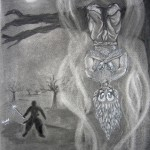
\includegraphics[width=.3\textwidth]{Vetal-150x150.jpg}
\end{wrapfigure}


To paraphrase a Scottish poet, perhaps no other word, other than those of \emph{Liberty} or \emph{Christ}, have been subject to as much abuse as the word ``\emph{Reason}``. These days the word \emph{Reason} has been defined to objectively exclude the very possibility of higher Intelligence, or higher Logos. At best, dialectical Reason (of the kind that American liberals imagined Socrates to be engaged in, illustrated by the career of Scott Buchanan\footnote{\url{http://en.wikipedia.org/wiki/Scott_Buchanan}}) is allowed to achieve the suspension of \emph{Aporia}. John Rawls\footnote{\url{http://en.wikipedia.org/wiki/John_Rawls}} embodied or re-embodied a lot of the vigor left in classical modern liberalism by restating Hobbes and Locke's contractual theory in a way that Buchanan might have found congenial, given as he was to attempts to re-invigorate the social ``federalism'' of the early American republic. This is the area which the great critic Richard Weaver termed ``the excluded middle'', and he argued that much of liberalism ``dances about in it''. At the other end is the view that ``reason is what the mind uses, and the mind is what the brain does'': this view is increasingly popular in a ``rational'' era. The term ``reason'' in either case (though far more malignantly in the latter) substitutes in such a way as to obliterate (like a lunar eclipse) the obviously solar presence of higher Reason. On the contrary, anyone who experiences an illumination (greater or lesser) finds that the experience is finding one's self, and simultaneously experiences finding something that is already thought (utterly rational) and yet utterly free (alive and imparting life and therefore freedom). So the sum of the experience is supra-rational. This would not seem to be such a controversial point, as it is well within the intellectual capacity of a hard-working twelve year old, but in the modern West, it appears to be so. It also happens to be the united and universal testimony of the best human beings of all higher cultures, and even of many of those which are not ``higher'', which explains why the burned out dregs of liberalism often turn to the lowest common denominator they can find among the outskirts of Tradition, in the form of the New Age or noble savagery.

In the tale of \textit{Vikrama and Vitala}\footnote{\url{http://en.wikipedia.org/wiki/Baital_Pachisi}}, the king captures a vampire at the behest of a treasonous tantric sorcerer, who intends to use both of them to overthrow legitimate authority. The tale is instructive, as it points out that illegitimacy lurks not in the most obvious evil, but rather in the moralistic facade of the cunning and clever, who see an opportunity for advancement at the expense of those who do not ``know''. The king is saved by listening to the captive vampire, who reveals the plan of the sorcerer and suggests a manner to overcome him. In this fable, it is seen how superstitious ``Reason'' has actually become, because it denies both the authority of the Emperor and attempts to master the black arts in Saruman-like fashion in order to augment personal power. Is it not superstitious to deny the fullness of God's Creation, and to make taboo and totem out of whatever is accidentally congenial to one's bent? The natural authority of the secular ruler and realm of the supernatural are both to be subjugated to the desires of the sorcerer-state, a theory of politics which one actually finds expounded in the works of Culianu\footnote{\url{http://thearchdruidreport.blogspot.com/2011/10/plutos-republic.html}}. We can see how ``Reason'' in the modern world, both as the prostitute and the ostensible mistress of Science and Justice, is similar to the thaumaturgic tantric-sorcerer of the Legend.

As great a poet, humanist, and thinker as Voltaire was seduced by the charms of secular thaumaturgy. It is a well known fact that the sublimated erotic rivalries of great thinkers and rulers who are legitimate often become mimicked in miniscule through their disciples, who are unable to appreciate the full scope of their work, but certainly key in on the tensions of their desires within the rivalries. Phillip Rieff drew attention to this in his work on \emph{Second Death}\footnote{\url{http://www.amazon.com/Fellow-Teachers-Culture-Second-Death/dp/0226716449}}. Thus, \emph{Voltaire's Bastards}\footnote{\url{http://www.amazon.com/Voltaires-Bastards-Dictatorship-Reason-West/dp/1476718962/ref=sr_1_1?s=books\&ie=UTF8\&qid=1423888644&sr=1-1&keywords=voltaires+bastards}} come to dominate the mental landscape of the West. Poor Voltaire wrote entertaining fiction like Candide, but never really (and self-confessed this) came to resolve the problem of Evil, and had to be content with living like a parasite off the ruins of an Age he helped to destroy. Don't end up like him.

The only way out this impasse is not to partake of the fighting in the rubble and ruin of the Western mental landscape, which is at this point dominated by the bastards of Reason in various titanic forms: there are the scientific crowds who can't accept something unless it can be explained in its most reductive terms, there are the masses of political factions who believe that the one burning question right now is to catalyze some form of resistance to the spread of whatever alien idea they define themselves in opposition to, there are the groups of people who endeavor to ``dance about in the excluded middle'' and prop things up by appealing to something along the lines of
\emph{Religion Within the Limits of Reason Alone}\footnote{\url{https://en.wikipedia.org/wiki/John_Toland}}, etc., etc.

No wonder Gornahoor lays so much emphasis on avoiding dialectical quarrels with those who don't share aims and principles, getting things right at the foundation, and putting practice into theory (and vice versa) from the beginning, so that one is most assuredly not at the behest or beholding of a salary, an occupation, or a career of some sorts. These webs of A influences (legitimate in their own way, but self-canceling in the sense that they operate mechanically through humans under their sway) will eventually reduce what they master to rubble, much like the current landscape seems to be vividly illustrating.

Those who want to find something that Russell Kirk called \emph{The Permanent Things} would do well to model their lives more on the life of a king Vikrama, who was brave enough to face vampires, and wise enough to listen to what he learned and avoid the trap that had been set for him. A young man could do much worse than aspire to the heroic and respect the supernatural -- or, as Jesus put it, to be wise as a serpent, but innocent as a dove. The alternatives seem to be being part of the Sheeple, or aspiring to rule over them as a sorcerer.


\flrightit{Posted on 2015-02-13 by Logres}


\section{The Seven Sacred Liberal Arts}

It is no coincidence that the Sacred Liberal Arts are Seven in number: this is the number of the mysteries, the steps towards union with God\footnote{\url{https://www.gornahoor.net/?p=10801}}, and the rays of Creation, as well as the visible planets, the notes in the musical scale, and the steps or levels of the Kabbalah. There are also seven deadly sins. We can collate some of them, as follows:

\begin{longtable}{*{5}{p{.15\textwidth}}}
	\caption{Correspondences between seven qualities}\\
	\toprule
	\textbf{Liberal Art} & \textbf{Augustine's Stage} & \textbf{Ray}\footnote{\url{https://www.theosophical.org/files/resources/books/SevenRays/SevenRAys.pdf}} & \textbf{Mystery} & \textbf{2 Peter}\footnote{\url{https://www.biblegateway.com/passage/?search=2+Peter+1\%3A5-7&version=KJV}} \textbf{Beatitudes} \\
	\midrule
	\endfirsthead
	
	\toprule
	\textbf{Liberal Art} & \textbf{Augustine's Stage} & \textbf{Ray} & \textbf{Mystery} & \textbf{2 Peter Beatitudes} \\
	\midrule
	\endhead
	
	\midrule
	\multicolumn{5}{r}{\textit{Continues in next page}}\\
	\endfoot
	
	\bottomrule
	\endlastfoot
	
	Grammar & Animation & Freedom and Action & Washing of Feet & Faith-Virtue \\
	Logic & Sentience & Unity and Philanthropy & Scourging & Virtue-Knowledge  \\
	Rhetoric & Rationality & Com\-pre\-hen\-sion and Philosophy & Crown of Thorns & Knowledge-Self Control  \\
	Arithmetic & Virtue & Harmony & Bearing the Cross & Self-Control-Steadfastness \\
	Geometry & Ataraxia & Truth and Scientist & Mystic Death & Steadfastness-Godliness \\
	Music & Intuition & Goodness and Religion & Entombment & Godliness-Brotherly Affection  \\
	Cosmology & Union with God & Beauty and Art & Resurrection & Brotherly Affection-Love \\
	
\end{longtable}


The liberal arts presuppose high intelligence, as the personal consciousness of the practitioner has to have already gotten as far as to see that there is no conflict, in the end, between Faith and Reason: since intellectus is destined for reunion with God just as surely as is purest faith. The union is effected in the consciousness of the just, or those made just. Those addicted to disputations or dilettantism will find the way of participation barred by the nature of the realities handled by the art. For those willing to re-engage them, the position and order of the seven liberal arts is teaching something about what its spiritual purpose is: it does this by the \emph{analogia entis\footnote{\url{http://www.millinerd.com/2006/12/whos-afraid-of-analogia-entis.html}}}, the law of correspondence, and the doctrine of signatures. The above table is a start.

For example, Mouravieff's Man \# 3 is a man of rhetoric (ideas); he engages the world intellectually, even when acting emotionally or instinctively, he uses the intellectual sectors with emotional or instinctual coloring heavily. Such a man would need to beware traps of rhetoric, and also study to engage more deeply in the truest and best use of creative rhetoric. Rationality, self-control, and the ``crown of thorns'' (the crucifixion of the intellect) would be things most necessary for this initiate to attend to in his self examination and training. He would attend to them knowing that they were his greatest strength, and also his greatest weakness, whereas weakness in the other disciplines would manifest completely differently: they would either be far more obvious, or far less -- A man \#3 would either be grossly deficient in the emotional arena, or (perhaps), far less tainted in that area (than in the intellect), and more artlessly or naturally pure, simply because it was not the seat of his ego, and precisely because it had been less ``developed''. Indeed, even in the exoteric literature, we find references to wisdom like this, as for example John Cardinal Newman recommending the benefits of liberal education\footnote{\url{http://www.newmanreader.org/works/idea/index.html}} for distracting the mind from idleness or temptation to fear, which is the besetting structural sin of a Man \#3.

Therefore although Geometry seems like a strange subject to study to develop one's spirituality, this is the ineluctable conclusion one is led to when delving into the interiority of man. For example, Thomas Hobbes came to Geometry\footnote{\url{https://www.uh.edu/engines/epi2372.htm}} rather late in life, and it shows in his thought, as illustrated in this amusing story:

\begin{quotex}
He was 40 years old before he looked on geometry; which happened accidentally. Being in a gentleman's library, Euclid's Elements lay open, and ``twas the 47 El. libri I'' Pythagoras' Theorem . He read the proposition . ``By God'', sayd he, ``this is impossible:'' So he reads the demonstration of it, which referred him back to such a proposition; which proposition he read. That referred him back to another, which he also read. Et sic deinceps, that at last he was demonstratively convinced of that trueth. This made him in love with geometry.

\flright{Quoted in \textsc{O L Dick}, \textit{Brief Lives} (Oxford 1960); A quotation about Thomas Hobbes by John Aubrey (1626-1697)}
\end{quotex}


Another observation that shows the non-arbitrary nature of the patterns in the Logos: the feet are the lowest part of the body, but also closely connected to spiritual development. Incidentally, this is the basis of ``foot-washing'' and also why people's feet get cold first when they are dying. There is also the old Bible verse: ``How beautiful upon the mountains are the feet of him that bringeth good tidings, that publisheth peace; that bringeth good tidings of good, that publisheth salvation; that saith unto Zion, Thy God reigneth''. (Isaiah 52:7) Mouravieff cites in Gnosis the practice developed by a group associated with Karel Weinfurter, in Man's Highest Development\footnote{\url{https://archive.org/details/manshighestpurpo032199mbp/page/n10}}, which details spiritual exercises designed to center development on the feet. The Middle Pillar Exercise\footnote{\url{https://www.golden-dawn.com/eu/UserFiles/en/file/pdf/Middle\_Pillar.pdf}} in Rosicrucian magic is a kind of ``grounding'', as well. Both exercises are a kind of magical ``Grammar'' (and Arithmetic). They are initiatory. And so can all the sacred liberal arts.

An entire program of spiritual and emotional and intellectual development is laid out in the Trivium and the Quadrivium, leading (finally) to union with God as its ultimate end. We can see that this seventh branch of the table is the highest plane of existence. The matching tables could make this very practical and specific. This seven fold pattern should be tried in a spirit of expectant humility: the numbers are not arbitrary.. He who maintains this out of sheer ignorance has not graduated the very first stage of instinctual life: the protozoa are more intelligent, in that they do better arithmetic with their instincts, and better grammar with their participation in Logos. The ignorant sceptic sorely needs the sacred liberal arts.

Recognizing the inner meaning of the liberal arts frees it from endless debates around the exact and minute particulars of the ``Canon'': it is less important what is precisely ``in'' (or ``out'') of the Canon, than in whether or not whatever is being studied shares a certain inner pattern and spirit. For example, \emph{Faust} is a Western classic. However, there are other obviously acceptable substitutes\footnote{\url{https://en.wikipedia.org/wiki/The_Tragedy_of_Man}} : someone can get an education from very few books, if they are ``right'' for their inner development. The development of depth in the pupil means a student of the \emph{Bhagavad Gita} and a disciple of the Gospel of John could hold a conversation and understand one another, because they share a deeper inner language. Canon details, provided they follow a pattern laid down by the Logos, are authentic and true. Esoteric recovery of the Liberal Arts will re-vitalize them, and save us from snobbery or dilettantism, or irrelevance.

Some will admit that the numerical pattern is interesting, but will find the details too speculative and abstruse. They are not cynical so much as possessing an over-developed worldliness. But their skepticism is even more difficult to address. Still, we can try to see if we can aid them, tossing a bone\footnote{\url{https://www.npr.org/templates/story/story.php?storyId=11803762}}:

\begin{quotex}
SIMON: I -- do you have any idea how seven became a lucky number?

Prof. DEVLIN: I have no idea, whatsoever, except that, you know, if we forget lucky numbers, there is a mathematical notion called a happy number. To get a happy number, you look at the number and you start squaring the digits and adding the answers. If you keep on doing that, eventually either you'll end up with the number one or you will end up getting a sequence of numbers that cycles. It begins 4, 16, 37. Seven is the smallest number that gives you one.
\end{quotex}


As you see, this is exactly the kind of stuff we find in Iamblichus' \textit{The Theology of Arithmetic}\footnote{\url{https://archive.org/stream/iamblichus-theologyarithmetic/iamblichus-theologyarithmetic_djvu.txt}}, which is dismissed today as risible. After leafing through the chapter on the Hebdomad (Aquinas commentated on Boethius' commentary\footnote{\url{https://www.amazon.com/Exposition-Hebdomads-Boethius-Aquinas-Translation/dp/0813209951}} on the Hebdomad), I did a little research, to see if I could find out what Iamblichus meant by calling 7 a virginal number. As it turns out, it is similar to seven being a ``happy'' number:

\begin{quotationx}
Evidence A\footnote{\url{https://books.google.com/books?id=udptayxY2E8C\&pg=PA27\&lpg=PA27\&dq=hebdomad+athena+virgin+iamblichus\&source=bl\&ots=2mH2dyjQgG\&sig=ACfU3U1fwbHMQmhzoZ67D8M2Hfwa4CJ_qw\&hl=en\&sa=X\&ved=2ahUKEwjQjZ60q-HhAhUNVa0KHTmLBI0Q6AEwC3oECAcQAQ\#v=onepage\&q=hebdomad\%20athena\%20virgin\%20iamblichus\&f=false}} (this source is derisive, but gives a valuable tidbit)

Other numbers arise naturally, but seven is ``left out'': 1-3 are generated by the point, the line, and the plane, and 4 is generated by the solid. 3 \& 4 then generate 5 in the Pythagorean triangle as hypotenuse, and 6 as the area, 8 is the first cube number, and 9 the first square. But Seven is nowhere to be found ``in mathematical nature'', except by intention.

Evidence B\footnote{\url{https://books.google.com/books?id=ifrHAAAAQBAJ\&pg=PA161\&lpg=PA161\&dq=virgin+seven+iamblichus\&source=bl\&ots=kef3A0I8kF\&sig=ACfU3U2Q5NAMgciQ-tERPOxlYWPxU5vmRA\&hl=en\&sa=X\&ved=2ahUKEwisq7e3ruHhAhUJvKwKHe0TAjUQ6AEwAHoECAkQAQ\#v=onepage\&q=virgin\%20seven\%20iamblichus\&f=false\%20target=}}

Agrippa states it is the only number that both 1) when multiplied by another number, produces none of the numbers in the decad (unlike 5, as in 5*2=10), and 2) is not the product of another multiplication of another number (only 1*7=7). So it has ``no father or mother''.
\end{quotationx}


Mathematics hasn't been affected by ``Modernity''. At least not in the qualities of the elemental numbers. The conclusion has to be that Seven is a repetition of One: It is Unity, Recreated and Manifested in fullness or perfection. Consult Genesis 1. Even the French Revolution had to go back to the days of the week.

Yet what other meaning could the numbers possess, if not to direct our attention to a particular spot, for deepening wisdom? For those lacking the arithmetical instincts of the amoeba or average honeybee because they deprive themselves, consider the alternative, which is that learning has no pattern, and no symbolism, but is purely utilitarian or even existential. Under this view, there is nothing requiring a leading out ``from'', and nowhere to quest ``towards''. Such positions all too obviously lead to nihilism, because if you destroy the symbolism of numbers, you are left with Zero. Others will find it somewhat fanciful, perhaps -- But why 7 and not 12? Or 21? What is the meaning of Life? You may as well answer 42\footnote{\url{https://www.independent.co.uk/life-style/history/42-the-answer-to-life-the-universe-and-everything-2205734.html}}! or else take Iamblichus seriously.

So certainly, each number ``means something''; they are something: thus, there are other numbers and patterns and meaning ``after'' 7, just as there are meanings for before 7. Since the intersection between Macrocosm (Triad) and Microcosm (Universe of ``4'') is 7, this has radical implications for education and spiritual development: our forefathers knew this in some way, whether instinctively, by experience, esoterically, or otherwise. Twelve (of course) results from the multiplication of 3 and 4, and is therefore just as significant as 7. And if we know how months differ from days, we have a clue to answer how. Perhaps the liturgical year could be brought into relation with the Liberal Arts? There are other things to say about the Numbers of course, all of them, and someone else could say more of 7. So the pattern can be enriched and expanded.

If God created the world by wounding himself and withdrawing to make the Void, then our imperfection is a task for both Him and our selves to overcome and finish the Creation, for God is at rest (He is perfect). He rests, having become man and overcome death, so that we might become God. God is, therefore, ``at work'' through us in our imperfection. He is perfect, and yet (on the human plane of activity), imperfect, since the revealing of the sons of God is not yet here:

\begin{quotex}
Praeterea, ostensum est supra quod essentia Dei est ipsum esse. Sed ipsum esse videtur esse imperfectissimum, cum sit communissimum, et recipiens omnium additiones. Ergo Deus est imperfectus. Objection 3: Further, as shown above (Question\footnote{\url{https://dhspriory.org/thomas/summa/FP/FP004.html}}3 , Article 4 ), God's essence is existence. But existence seems most imperfect, since it is most universal and receptive of all modification. Therefore God is imperfect.
\end{quotex}


Aquinas goes on to deny that God is imperfect (he answers this objection), yet there is an inner meaning to the old verse: And He said to me, ``My grace is sufficient for you, for My strength is made perfect in weakness (I Cor 12:8-10). What is this making perfect, if not God taking on imperfection, to suffer with those humble or pure enough to be of His mind, in order to further creative spiritual evolution?

Thus, the liberal arts are the strength of God for our weakness of mind, yet they are simultaneously nothing compared to the strength of God that they lead towards. For once completed, they are fulfilled: ``He who finds truth, beauty, and goodness, finds more'' (Dr. Michael Baumann). This is why Aquinas on his deathbed said\footnote{\url{http://scriptoriumdaily.com/thomas-aquinas-big-pile-of-straw/}}:

\begin{quotex}
I adjure you by the living almighty God, and by the faith you have in our order, and by charity that you strictly promise me you will never reveal in my lifetime what I tell you. Everything that I have written seems like straw to me compared to those things that I have seen and have been revealed to me.
\end{quotex}


Part of our task requires us to avail ourselves of a rational and sound mind, and to think God's thoughts after Him. In order to transcend humanity, we have to develop our humanity up to its natural limit: the common saying in parlance is, Put Wings to your Prayers. Trust in God, tie up your camel.

Sharpening the mind in, through, and on the sacred liberal arts, allows the fastest progress in developing the intellect up to its natural limit.

Hopefully, more work will be done in recovering the basis of the Seven Sacred Arts. The orders of angels comes to mind, as does Bonaventura's Journey of the Mind into God\footnote{\url{http://www.ntslibrary.com/PDF\%20Books/Bonaventure\%20Journey\%20of\%20the\%20Mind\%20Into\%20God.pdf}}: for example, if you add philosophy and theology to the seven liberal arts, you have 9, which is the order of the angels. A young scholar aspiring to be a sage could do worse than undertake the revitalization of the Sacred Seven Liberal Arts. Interest in it is already increasing, as evinced by this recent article\footnote{\url{http://www.tomworrel.com/uploads/3/4/7/9/34794642/ahiman_worrel_article_page_7-37.pdf}}. The table provided at the start, along with the esoteric background, may be of very practical use. Our forefathers, even a hundred years ago, had not entirely forgotten that the edifice of civilization is built, not on Mammon, but on something much deeper. They even carved it into stone\footnote{\url{http://www.studiesincomparativereligion.com/uploads/ArticlePDFs/403.pdf}}, so we could not forget.

Hopefully, we have scratched the surface enough in the above to demonstrate that there is a deep organic inner Logic behind the tradition and lay out of the Seven Sacred Liberal Arts, enough to get you interested, and started. It's just a beginning.


\flrightit{Posted on 2019-05-05 by Logres}

\begin{center}* * *\end{center}

\begin{footnotesize}
\begin{sffamily}
\texttt{Zach on 2019-05-09 at 21:15 said:}

Thanks. This came on a significant day for me.

Although I am well past being a ``young scholar.'' The Hobbes anecdote is hopeful.

\hfill

\texttt{Logres on 2019-05-12 at 00:20 said:}

I like the quote that Cologero put up recently, that the young learn from us what we've learned by heart (I can't remember the name of the Frenchman quoted). Falling in love with it, or all over again, helps us learn it by heart. Maybe you can help pass it on. Thanks for reading.

\end{sffamily}
\end{footnotesize}



% Jámblico
\section[The Theology of Arithmetic]{A commentary on The Theology of Arithmetic by Iamblicus}
\subsection{Fortune’s Fool by Numbers}

\begin{quotex}
But I think about the hebdomads for myself, and I keep these speculations in my memory rather than sharing them with any of those people whose impertinence and insolence permits nothing to be analyzed without joking and laughter. Accordingly, don't be opposed to obscurities stemming from brevity; since they are the faithful guardian of the secret they have this advantage: they speak only to those who are worthy. Therefore, as is the customary practice in mathematics and also in other disciplines, I have first put forward terms and rules, in accordance with which I shall work out all that follows.
\end{quotex}


Boethius likely had a connection to esoteric doctrine via the Pythagoreans (his mundane connection to neo-Pythagoreanism is considered by scholars to be settled). He was a ``classically educated'' man, but as Miranda Lundy points out the four sciences of Number, Music, Cosmology \& Geometry were actually formerly \emph{sacred} sciences, and most definitively not a preparatory or prerequisite curriculum for anything else except sacral or transformative theology or philosophy. Sarah Lassin argues that Boethius' reference to the Egyptian ``hebdomads''\footnote{\url{http://individual.utoronto.ca/pking/translations/BOETHIUS.On\_the\_Hebdomads.pdf}} (which plays an important role within the Neopythagorean literature of Hierocles and Nicomachus of Gerasa\footnote{\url{http://books.google.com/books?id=dCELAAAAIAAJ\&pg=PA94\&lpg=PA94\&dq=nicomachus+hebdomads\&source=bl\&ots=TnzwHveyQF\&sig=ENK2-4LKLaMFDcxMhWkQdBwkqf0\&hl=en\&ei=wwPOTd6wN8PngQevmLihDA\&sa=X\&oi=book_result\&ct=result\&resnum=3\&ved=0CCoQ6AEwAg\#v=onepage\&q\&f=false}}) is highly significant for the discussion of God \& creation. In fact, it is not necessary even to mention the Egyptian origins of these terms, since Proclus discusses them\footnote{\url{http://books.google.com/books?id=z-M-AAAAYAAJ&pg=PA316&lpg=PA316&dq=hebdomads+triads&source=bl&ots=7lW956x_Vy&sig=77Nd93YLZNUyh5LvWP3foh-9FME&hl=en&ei=TKXMTZfrFYK4tgfn_u2WBQ&sa=X&oi=book_result&ct=result&resnum=1&ved=0CBYQ6AEwAA\#v=onepage&q=hebdomads\%20triads&f=false}} extensively on Plato, and Plato (and also Herodotus) thought that the Greeks derived much of their mysteries from Egypt. The Egyptian context\footnote{\url{http://www.sofiatopia.org/maat/ten_keys.htm}} makes the connections between philosophy and religion even more apparent:

\begin{quotex}
Hermes tells Tat (XIII), that ``the tent'' or ``tabernacle'' of the Earthly body was formed by the circle of the Zodiac (XIII.12 \& Ascl.35) and dominated by fate, who's decrees, according to the astrologers, were unbreakable. The seven planets represented the ``perfect movements'' of the Deities, the unalterable ``will of the Gods'' as expressed in predictable astral phenomena. Magicians tried to compel this will, while Hermetism did not try to resist fate, but irreversibly. The existence of the Deities was acknowledged (they belonged to the order of creation and were the object of sacrifices and processions and the celestial Powers ruling the astrological septet). Indeed, the Deities, Hermes and God were situated in the eighth, ninth and tenth sphere (Ogdoad, Ennead and Decad). The ``eighth'' involved purification, Self-knowledge and the direct ``gnostic'' experience of the ``Nous'' as ``logos'', whereas in the ``ninth'' man was deified by assuming God's attributes, as did the Godman Hermes, in particular His Universal Mind, the Divine Nous, Intellect or ``soul of God'' (XII.9). The ``tenth'' or Decad was God Himself for Himself.

\end{quotex}


And the Egyptians mysteries are linked to Hermes Trismegestus, which context resurfaces during the Renaissance when Greek translators made the Emerald Tablet available in Italy. This Egyptian link might also explain the persistence at Alexandria of a Christian esoteric tradition- Alexandria is also the home of the tragic conflict concerning Hypatia and the library, a conflict that did not occur until the Greek influence had waned in the Church.

Given that Boethius was the schoolmaster of medieval and early modern Europe, one might almost say that these doctrines ``sub-created'' Europe. Thomas Aquinas discusses\footnote{\url{http://individual.utoronto.ca/pking/translations/AQUINAS.Exposition\_of\_Hebdomads.pdf}} Boethius and the hebdomads in a treatise, \& it is instructive to compare the two discussions\footnote{\url{http://individual.utoronto.ca/pking/translations/BOETHIUS.On\_the\_Hebdomads.pdf}}; by Aquinas' time, the debate is far more abstract and limited to logical distinctions, as opposed to being ``transformative''.

As perennialist studies on Boethius\footnote{\url{http://www.studiesincomparativereligion.com/Public/articles/Boethius\_Three\_Musicians-by\_Joscelyn\_Godwin.aspx}} make clear, his theories of music and number (as found in minor tractates) gives a better background for the dialectic that occurs within theConsolation of Philosophy. Boethius was not simply a well-informed ``liberal'' who opposed barbarian elements at Court --- he was a lover of wisdom who was in an intimate and self-converting dialogue with Sophia herself, one who was willing to pay the final price for that which he had found and was finding\footnote{\url{http://www.hermes-press.com/philosophy\_emboldening0.htm}}.

\begin{quotex}
During the Dark Ages in Europe, acquaintance with the works of Plato was at second or even third hand, through the writings of authors such as Macrobius, Martianus Capella, Augustine, Boethius, Calcidius' translation of the \emph{Timaeus}, and John Scotus Erigena. The most important contribution in the vernacular was provided by the late ninth century reworking of Boethius' \emph{De consolatione Philosophiae}.
\end{quotex}


\emph{The Emboldenment of Philosophy} became one of the most popular books throughout the Middle Ages. It was translated into Old English by Alfred the Great, into Middle English by Chaucer, and into Elizabethan English by Queen Elizabeth.

As we see from Proclus' statement, the Neo-Platonists emphasized dialectical interchange in their transmutational teaching procedures within the Perennial Tradition--one of the important components of the Wisdom Teachings. However, the first Perennialist teacher who initiated and developed all facets of the Wisdom Teachings was Anicius Manlius Severinus Boethius (480-524 C.E.), including in his teachings and life experience each theme and emphasis we've outlined above.

While in prison awaiting a ghastly death, Boethius had experienced a definite inner dialectical interchange between his soul and Lady Philosophy (the spirit of the love of Wisdom). The narrative account in his \emph{Emboldenment of Philosophy}\footnote{\url{http://www.hermes-press.com/philosophy\_emboldening0.htm}} discloses how Boethius achieved transformation and self-understanding while communing with Lady Sophia in an inner spiritual domain. Boethius' book combined verse and alternating dialogue between himself and Lady Philosophy, organizing his narrative into different stages of his spiritual healing and transmutation. Lady Philosophy communes with Boethius in his inner being, bringing into the dialectical interchange others who were true devotees of philosophy: those who love and seek Wisdom.

The wisdom school of the Pythagoreans was influential enough that Augustine made an appeal to those who ``knew'' to the effect that the Hebdomads symbolized the perfection which was to become the Church, which was to rely in almost exclusive fashion\footnote{\url{http://orthodoxnotes.com/wp-content/uploads/downloads/2010/06/Liturgical-Practice-in-the-Fathers.pdf}} upon the mystery religions, perhaps even more than on Judaism, for the new doctrines. Christianity began as a conversion of existing elements, rather than a superimposition. Augustine's appeal is a sincere one.

Given that Boethius' interests in music and number coincide with Platonist streams of thought in Proclus and Plotinus in the Pythagorean mysteries, it is necessary to think that the esoteric link which created the Middle Ages through Boethius could be located in the harmonics and sacred geometry\footnote{\url{http://www.sacred-texts.com/eso/sta/sta19.htm}} of the celestial ``music of the spheres''. In order to understand the Middle Ages, we should ``close thy scholastics, and open thy Timaeus''. Boethius' background and writings, embodied in the \emph{Consolation}, are an excellent place to re-start.



\flrightit{Posted on 2011-05-14 by Logres}

\begin{center}* * *\end{center}

\begin{footnotesize}
\begin{sffamily}
\texttt{logres on 2011-05-14 at 22:39 said:}

This is a good example of impasse between ``orthodox'' and ``gnostics'':

\url{http://www.interfaith.org/forum/livergoods-esoterism-10888.html}

Trajan's orders seem reasonable from a political standpoint -- the Christian response was muted and in accord with Romans 13. However, it is clear that persecutions of the faith quickly became excessive. This probably gutted much of the leadership. If the Corpus Hermeticum dates from the 3rd century, then it is the obverse of the same coin which Clement was minting.

The chance was missed. And is still being missed. That is why Boethius is so important. In spiritual war, as in physical, it is often the best that are lost. To tie into Cologero's posts, there is still an opportunity perhaps even today to refashion Romanity as a vehicle, in the Catholic Church. If the chance is missed again, we will simply behold a repetition of the pattern, until what is meant to happen, what is already one, is manifest. From the debate linked above, it's clear that Mouravieff's Gnosis is an important tract.

\hfill

\texttt{Spock on 2011-05-15 at 09:40 said:}

logres, you say there is still a chance to fix the church, well yes, we can say this forever, but the truth is that leading perennialists have had continuing dialogues with the recent popes and it changes absolutely nothing because the church is and will only be a political vehicle which panders to its supporters... none of whom are even remotely interested in gnosis and tradition. What they love are superficial rituals and the joy of submission to authority, because they do not love wisdom, they would rather be told and given things like children rather than do the task themselves. That in itself in contrary to the active gnostic life. If one really wanted to change the church he must first change the people, but that is the impossible task in this the last phase of the kali yuga.

\hfill

\texttt{James O'Meara on 2011-05-15 at 10:10 said:}

Freke and Gandy quote modern scholarship to show that the persecutions were quite minor, both in time 5 years, total and numbers 10 killed in Alexandria! ; Origen is quoted to the effect that the number of `martyrs' was `easily counted'.

\url{http://tinyurl.com/5v7w5nv}


The ``great persecutions'' could hardly have `gutted much of the leadership'' although the orthodox literalists did a pretty good job decimating the Gnostics and other `heretics'.

As always, the primitive Christians seem to specialize in self-serving propaganda and literary fakery the letters of Jesus to Pilate, anyone? . Speaking of which, interestingly, the Gnostics rejected the ``pastoral epistles'' as spurious, just as modern critics do, while Irenaeus insisted on them, showing his unerring eye for self-serving fakery, and proving that Guenon was wrong to dismiss Biblical criticism as a modernist evil. Even today, listening to radio preachers, it's amazing how much of their bible-thumping comes from Timothy, Titus and Peter, plus a whole heaping helping of Apocalypse. ``Modernist criticism'' would disarm a lot of the Protestantism Guenon opposed.

\hfill

\texttt{logres on 2011-05-16 at 08:58 said:}

It wouldn't surprise me to find out the persecutions were exaggerated -- however, I can't find footnote 138 (and those next to it), to see which scholars they are citing. The argument doesn't really depend upon who killed whom, but rather upon ``elective affinities''. Certainly, it is possible that the Church became exactly what She portrayed Rome as being. Tomberg, Mouravieff, etc. aren't trying to esoterically ``capture'' the exoteric Church as it has developed (which is splitting up all on its own into fragments) but to reunite those elements which should be (and are) One. So I don't think it matters what the overly visible Church does. At least not for purposes of working in the areas of Form.

However, it certainly matters to set the record straight, if what one means by that is to revisit assumptions which one thinks one knows, and for the purposes of refuting aggressive error. Thanks for drawing attention to this issue.

\hfill

\texttt{logres on 2011-05-16 at 09:04 said:}

The Church (in other words) is not only the people, and perhaps in a sense not the people at all. A difficult task, I know.

\hfill

\texttt{logres on 2011-05-18 at 22:03 said:}

B16 speech on Proclus \& Pseudo-Dionysius:\\
\url{http://www.zenit.org/article-22588?l=english}


\hfill

\texttt{Dimitri on 2022-06-30 at 19:18 said:}

Though it has been over a decade since his comment was posted, I would still like to correct Mr. O'Meara's many errors (which stem in large part from his relying on the absurdities of the so-called ``Christ myth theorists'' as a source). In his first point, he claimed the persecutions of early Christians were exaggerated. This is somewhat true to an extent, though they were nowhere near ``minor'' like he claimed. He gives the impression that there were perhaps a few dozen people killed and that the overall period of persecution was very short, but if only he had done his research he would have seen just how wrong he is. How he arrived at the idea that persecution only lasted for ``5 years total'' is beyond me, since even if we were to only include imperially ordered persecution, we would still arrive at a total of 13 years of persecution under Decius, Valerian, Diocletian and Galerius. And this is only if we exclude the many local persecutions where Christians were attacked by regular people without any official orders, or were persecuted under various governors whose authority was limited to specific regions of the empire. For the first century or so after the beginning of Christianity, Christians were fairly unpopular with the people and had to avoid the public sphere. But beyond this, O'Meara also greatly downplays the death toll even from the imperial persecutions. The Diocletianic Persecution alone claimed well over 3000 lives, even according to ``modern scholarship'' (and keep in mind that the number of Christians around then was smaller than it is today). There were many thousands of Christians martyred for their religion throughout the years, his deceptive use of Origen's statements notwithstanding.

As for whether ``\,`modernist criticism' would disarm a lot of the Protestantism Guenon opposed'', perhaps this is true, but it certainly doesn't replace it with anything worthwhile or meaningful. In fact, it seems to have made the situation worse, since we're now at a place where regular people (at least in the West, and this is especially true of Americans) see Christianity only through the lense of fundamentalism and mistakenly think that to be Christian they MUST believe in a strictly literal interpretation of all Scripture (among other errors) and have therefore forgotten the essence of the religion entirely. Perhaps the reason Guenon opposed it was because these ``critics'' and ``scholars'' do not really understand the contents or the implications of what they are supposed to be studying? For example, Cologero recently made a post about a scholar discussing how the Gospels were authored by a Christian elite (which would of course go against the ``traditional attribution'' to ``early eye-witnesses''), and yet from my experience this information would sooner be used in a polemical attack (as O'Meara himself tried to do here) by those who in their ignorance possess a vigorous contempt for what they think is Christianity than it would be to actually learn anything useful.

\hfill

\texttt{Dimitri on 2022-06-30 at 21:02 said:}

Actually, I realize now I forgot to mention the fact that ``modernist criticism'' itself only exists because of Protestantism and its nontraditional elements, such as its tendency for secularization and adherence to various profane ``philosophies'', and so it could hardly be an antidote to it. So not only does it not replace it with anything meaningful as I said before, but ironically it's similar to an Ouroboros, in that it's like a snake consuming itself.

\end{sffamily}
\end{footnotesize}


\section{The Dyad}

As we enter into the mystery of the One-and-the-Many, things begin to get more complicated. Even from Wikipedia\footnote{\url{http://en.wikipedia.org/wiki/Iamblichus}}, it is obvious (apart from the caveat that Iamblichus did not ``introduce'' any ``notions'' at all) that Iamblichus is essentially creating a parallel system that in many ways is similar to Christianity. This is why Julian the Apostate admired him so much, and why Porphyry disagreed with him so vehemently (Porphyry thought that purely notional contemplation ought to suffice for attaining divinization). From his doctrine of the One-and-the-Many, to his insistence that the lower types of men need physical theurgy, to his peopling the cosmos with various divinities and powers that are subject to Number, Iamblichus' world highly resembles that of the Church Fathers.

He introduces his doctrine of Dyad:

\begin{quotex}
So each thing and the universe as a whole is one as regards the natural and constitutive monad, but again each is divisible, in so far as it necessarily partakes of the material dyad as well. Hence the first conjunction of monad and dyad results in the first finite plurality, the element of things, which would be a triangle of quantities and numbers, both corporeal and incorporeal. For just as the sap of a fig tree congeals liquid milk because of its active and productive property, so when the unificatory power of the monad approaches the dyad, which is the fount of flowing and liquidity it instills limit and gives form (ie., number) to the triad. For the triad is the source in actuality of number, which is by definition a system of monads. But in a sense, a dyad is like a monad on account of being like a source.
\end{quotex}


The Dyad (therefore) is the Feminine Principle; in relation to the Monad, She is passive, as matter is to God. However, in relation to what comes after, by her productive powers, she is the Fount or Center of things, like a Monad, because in her Life originates (and multiplicity is created). This gives a good idea of the sophistication of Iamblichus' thought: ``opposition'' to the Monad (for him) doesn't mean resistance or lack of submission, but (precisely) submission through being opposite, or complementary -- in other contexts (the material realms) it is the Dyad that takes on the characteristics of the Monad: the Queen stands in the place of the King (one can't help but think of this doctrine\footnote{\url{https://en.wikipedia.org/wiki/Queen\_of\_Heaven}}, at this point).

I am not arguing that he is a pseudo-Christian, but rather that both Iamblichus and the Church Fathers were partaking of the same divine pattern, even (and up to) the particular manifestations of it at that time and place in history: see this article (for instance) as to how theosis and henosis\footnote{\url{http://web.archive.org/web/20080724183137/http://www.theandros.com/iamblichus.html}} differ, and how they do not. It might not be going too far to say that Iamblichus' teachings represent a possible locus for reconciling paganism with Christianity (by purifying paganism and refining Christianity), thus creating the possibility of \emph{\textbf{``white'' theurgy}}.


These possibilities arise from the subtlety of Iamblichus' method \& manner of dealing with the One-And-The-Many, as he unfolds a doctrine of the Dyad (II -- 2). Rather than posit a merely crude opposition, he shows how the Dyad is both Isis \& Ison, Equal and Unequal, Generator and Destroyer.

2, mathematically, is composed of 1s, and is therefore (from arithmetic linear) a Greater or Non-Equal. When viewed as a plane (2 squared), it becomes a Lesser, since 2 itself is less than 4. The undoubted metaphysical conclusion is that the Dyad contains elements of being both Greater and Lesser within it. This is an example of the kind of paradox that Iamblichus is seeking. The number 3 (as we will see) is the first truly diverse equal (1 is equal to itself, but is not diverse): 1+2 = 3, so that the preceding sequence of numbers added together is equal to the number itself. This is not true when we come to 4: 1+2+3 does not equal 4 (Iamblichus will draw conclusions from this, as well).

The Dyad has special properties (also) because 2+2 = 4, which is the same as 2 taken to the plane (2 squared). This is the only number like this. The Dyad is another Monad (being a 1 added to a 1), but the Monad does not generate this truth of equality between arithmetic and plane extension.

Yet in another sense the Dyad cannot create a plane figure, because two angles don't construct a plane figure: so the Triad is anticipated -- it alone can create planar figures. The Dyad, on the other hand, can construct infinity, in a sense, because it can create a line running from a point, indefinitely, in two dimensions. This line may, or may not, return to its Origin.

The Dyad, therefore, is not to be mistaken for the original Monad, despite its functioning in relation to other numbers as a Monad itself. This is because the Monad stands alone -- if, therefore, the Monad stands alone as Unity, something else has to take its place as the new principle of Unity to give unity to the other numbers. The Dyad, therefore, becomes ``Monadic'' towards the other numbers.

Numbers, therefore, inculcate the appreciation of metaphysical truths, such as the interplay between Microcosm and Macrocosm: the Moon or the Queen can become or stand in place of the Original Unity, precisely because of the primal unity of the One. Opposition can not exist, except to reinforce the One.


\flrightit{Posted on 2013-01-04 by Logres}

\begin{center}* * *\end{center}

\begin{footnotesize}
\begin{sffamily}
\texttt{Logres on 2013-01-05 at 06:17 said:}

Cologero points out to me that it is not really a matter of ``reconciling'' the Church Fathers with Iamblichus, \& I agree -- more a matter of seeking and finding the deeper unity which should be apparent, but tends not to be, due to modern habitus of thought.

\hfill

\texttt{Mihai on 2013-01-05 at 12:38 said:}

Thank you for this, Logres

\hfill

\texttt{Jason-Adam on 2013-01-05 at 14:21 said:}

More people need to read Tomberg if they cant understand what Gornahoor is doing IMO... ... ... .

Forgive my ignorance, but is the Dyad the same as the Demiurge in Plato ?

\hfill

\texttt{Logres on 2013-01-05 at 22:52 said:}

I don't have a good answer re: the Demiurge. Iamblichus is keen to insist that there are not ``two Monads'' -- however, the Dyad is Monadic by virtue of being different than the diverse numbers which follow. The Dyad itself is ``two monads'' (1+1). In Gnostic mythology, the Demiurge tends to be so powerful that the Monad is effectively relegated to mythology or the afterlife, so it overshadows the whole point, and refutes itself.

\hfill

\end{sffamily}
\end{footnotesize}


\section{The Triad}

When one refers to the Triad, one must remember that:

\begin{quotex}
The Triad has a special beauty and fairness beyond all numbers, because it is the very first to make actual the potentialities of the Monad -- oddness, perfection, proportionality, unification, limit.
\end{quotex}


We recall that the Dyad is a second Monad, which begins the process of the primordial's manifestation, which process reaches a form of completeness with the Triad; this is because the Triad is the first number to be ``odd'' (``Odd'' here meaning that when divided, one part is greater than the other, or differs from the other). It is the first number to be equal to its predecessors, because 1+2=3. Recall with the Dyad that all we can say is that it does not succeed the Monad in the same way that the Triad succeeds both Monad and Dyad, because 0+1= 1, not 2; the Dyad is an ``as-if'' Monad, not a true successor. With the Triad, a true harmony is reached.

In the Christian tradition, the Son does not claim equality with the Father, nor does He retain dominion and lordship at the end of time: rather, He delivers all back up to the Father, or Arche, through power of the Spirit. It is with the Spirit that true balance within the Trinity is reached: The Father generates the Son, and the perfect submission and harmony from the Son to the Father, the perfect Love for the Son from the Father, is so intense it generates a Third Person, and this forms the perichoresis of both inner essence and outer energies of the Divine ``Three-in-One''. The Son is associated with the Dyad, as is Queen Mary, the Queen of Heaven: Water, the most submissive element (as the Tao teaches) symbolizes the Feminine \& the baptism of the Son.

The Triad is unique in that 1+1+1=3, where the middle term is the same as the two extremes. Also, in 1+2+3, the middle term is equidistant from the two extremes. So it succeeds (perfectly) two sources, and is the system of the two sources. 3 exists between 2 and 4 in a special way, additionally: 2 is the first double, and sums up the idea of being ``greater than'' the One (0+1=1, less than 2), while 4 is sesquialter, that is, it is less than 1+2+3 (=6). 3, as pointed out, is precisely equal and balanced, because 1+2=3.

So we see the ``Son'' is highly exalted, although being perfectly submissive. The ``Son'' (2) is not successive to the number(s) preceding it (and is therefore less), while He is greater in that He is ``more'' or actualized, because He ``doubles'' the Father. This is the way it is expressed in Christian dogma, but Iamblichus is teaching something that is at the common root of this dogma with other traditions, seeing that even in Taoism, there is a Divine Three\footnote{\url{http://en.wikipedia.org/wiki/Three\_Pure\_Ones}}. We might say that Christianity is the religion of the Son, externalized, out of the bosom of the Father, but that the Monad retains the power and the glory to sustain, unmanifested and manifested, something else that shares the common root in that Monad. If this makes your head hurt, or sounds too Christian, just concentrate on the Numbers.

\begin{quotex}
The Monad is like a seed in containing within itself the unformed and unarticulated principle of every number, the Dyad is a small advance towards Number, but is not Number outright because it is like a source; but the Triad causes the principle of the Monad to advance into actuality and extension. `This' belongs to Monad, `either' to Dyad, and `each/every' to the Triad.
\end{quotex}


Iamblichus also uses etymology: Trein means piety, so it is called prudence \& wisdom; in the Christian tradition, Divine Sophia (as well as in Gnosticism). Knowledge (true knowledge) follows the Triad. The Triad is also beginning, middle, end. This is why prayers are made three times, in formulas of threes, and why even the Triangle (the first planar figure) has three different types (equilateral, scalene, isoceles). Adding the Triad up we get 6, which is the first perfect Number. It is unyielding and cannot be worn down, because you cannot divide it into two equal parts. There are three Fates, three levels of Creation (sky, land, water), three motions of the stars (summer, winter, ecliptic), and three phases of moon (waning, waxing, full). Giving, receiving, and requital is the pattern of Generation, both divine and human. He even quotes Homer: ``all is divided into three'', which becomes (with Aristotle) a meditation on virtue being the mean between two extreme vices.

What is crystal clear is that even something as simple as the relations of the very most basic Numbers is revelatory, to the meditative spirit, of the fabric of the universe. And this makes perfect sense, for how could God not be revealed in that which is most humble, the smallest of things, the very pebbles or calculi which we move around in our first attempts at numeracy?


\flrightit{Posted on 2013-01-11 by Logres}


\section{Heaven By Storm on the Number Seven}

I have paused, once more, at the Number Seven, for there are seven deadly sins which every mortal must purge themselves from, before the ascent, and there are seven corresponding virtues, four classical ones, and three theological ones, which (no doubt), ingenious readers can correspond in various ways to each of the deadly sins. The seven spirits which guard Heaven, and must be taken by storm, will fall with the aid of the Queen of Revelation, Mary, High Priestess of Heaven, who rules the lower waters and has become the upper ones. I have written several poems to her over the last year, and this one is from a fairy tale I am writing for my children, in which the main character is named Anna May, and who is acting as a symbol of Queen Mary, on behalf of those under her care.

\begin{verse}
\textbf{War in Heaven}

The angel sang her questions bold,\\
And Anna answered as of old.\\
The time was written, and was fitting:\\
Storm against the gods of old.\\
For many swarmed about that flood,\\
The evil, neutral, and the good,\\
Catching souls for food unholy.\\
Rulers in thrones and power most crude,\\
Each of the strong and original seven,\\
Held blades from world-heart riven,\\
They held the gap, and sealed the trap,\\
Which runs from earth to heaven.\\
Dozens under them, the decan twelve,\\
Hundreds beneath them, who delve,\\
Into the secret hearts, and inner parts,\\
Stubborn as dwarves, angry as elves.\\
They guard the purity of space,\\
From all the failure of the doomed race,\\
And test the ones, who dare the run,\\
Against the suns, into God's face.\\
Behold their wrath, how beautiful and strong,\\
Fashioned of our faults, our sins' song,\\
Their dreadful shade, from us is made,\\
They or us must die to free our wrong.\\
One cometh, shall come, always treading,\\
She who rules heaven, the wedding\\
Of the moon and sun, mercy-justice One,\\
Herald of a brighter Sun unebbing.\\
Who is this who faces the Seven?\\
Who is this warlike maid of Heaven?\\
First falls great Pride, and then Falls his Bride,\\
Envy who breathes the green fear-raven.\\
Lightning struck again, the maid grew proud,\\
Proud of how it must be done and loud\\
Grew the zeal of her heart, and the sword in art,\\
Struck through and through wrath's shroud.\\
Angry then, she sprang against the cherubim\\
Dark who mock despair of those in Lim:\\
Froze the fire of sloth with beauty wroth,\\
The silver fire rolled rippling through the Dim.\\
Peaceful now in dance she turns,\\
Calm she clasps the angel and she burns,\\
Lightning again, against the dun gods of sin,\\
Waning Greed falls as she yearns.\\
Two bolts more she snares of angel fire,\\
Herself she rules complete, a Lyre\\
She weaves and plays, the arrows ray\\
The one who makes wine a fire.\\
The last did fall as one long dead,\\
She of beauty great, but inward bled,\\
The terrible one, whose power to stun,\\
A fire within must quench instead.\\
Anna flickered fire and stood the queen\\
Of heaven cold that night, between\\
The living and the dead in fright,\\
She whom Sun and Moon made clean.
\end{verse}

\flrightit{Posted on 2013-03-01 by Logres}


\subsection{Octad}

The Octad is a short chapter.

Iamblichus continues his march\footnote{\url{http://www.scribd.com/doc/48888397/Iamblichus-the-Theology-of-Arithmetic}} through numbers noting that all men, without exception, count 1-10. The empiricist says this is because they have 10 fingers, and the Hermeticist says ``why do you suppose that is?''. In any case, it is not impossible to conceive attempts to circumvent divine order, such as the reordering of week days\footnote{\url{http://en.wikipedia.org/wiki/French_Republican_Calendar}} during the French Revolution, so their argument holds little water (which they know -- most of the Anglos don't use metric).

Eight is perfect, in that it is 1+7, neither number which is engendered, as Seven is a ``second'' Monad, in this meditation. The first two odd numbers (3 and 5) also produce it, making it relate to the process of the Cube (Claims Iamblichus, although he doesn't specifiy how this is so).

The pattern four is in the ecliptics of the Zodiac, and the ``circles'' (tropics and polar), as well as finding expression in Harmonic divisions and even the teeth and skulls\footnote{\url{http://en.wikipedia.org/wiki/Human_skull}} (presumably four big plates) of human beings. For instance, birds usually have four claws, and if an insect has more than eight legs, it is usually not exact.

\begin{quotex}
Philolaus teaches that after mathematical magnitude has become three dimensional thanks to the tetrad, there is the quality and `color' of visible Nature in the pentad, and the ensoulment in the hexad, and intelligence and health and what he calls `Light' in the hebdomad, and then next, with the ogdoad, things come by love and friendship and wisdom and creative thought.
\end{quotex}


So we are looking more now at what is normally understood as ``manifestation'' or ``Creation''. It is safety and foundation, because its root is in 2, and 2 is the leader of Manifestation in the sense of ``daring'' or ``courage'' (warrior-qualities).

There is a long section on harmonic relationships which is very involved with terms like sesquitertian, sesquioctave, etc., but I will recommend it to musicians, only noting for the Layman that what he needs to know is that the sesqui interval works as follows. 12 is the sesquialter of 8 (it succeeds 8 by an interval of half, so the ``change'' is related to the ``substance'' by law), and the sesquitertian of 9 (it succeeds 9 by an interval of one-third).

There is, of course, the Indian method\footnote{\url{http://www.sanatansociety.org/vedic_astrology_and_numerology/indian_numerology_8.htm}} of examining the birthday, name, and age of the person in order to use Pythagorean reduction to basic numerals to arrive at spiritual meaning. But these are more personal methods, and less metaphysical, than those which Iamblichus deploys.

8 resembles the infinity symbol, turned at a right angle. Does this mean that it is Infinity, set on its ear? In other words, Infinity set towards a downfall? Iamblichus does seem to indicate that ``manifestation'' in terms of Bios begins to break forth in 8, interweaving design and matter in actual genesis. We might think of the TV programs we were all indoctrinated on, which always start with some image of algae or lava or star dust, coalescing and shimmering and out-breaking, in order to appreciate the power of 8. The affinities are revealed: sex, division, mutual interdependence, etc.

Just for fun I looked up some modern\footnote{\url{http://www.youtube.com/watch?v=Adlw7sRw7cg}} numerology; Ellis Taylor seems to think that our Arabic numbers (in contradistinction to Latin ones, which are more pure) have been used to program us for failure. Although this sounds like the typical modern conspiracy theory, it may have something of interest, considering that even the Solfeggio\footnote{\url{http://www.miraclesandinspiration.com/solfeggiofrequencies.html}} scale has been reset in the modern Era. All changes of this sort ought to be more self-consciously investigated.

\begin{quotex}
Our modern day musical scale is slightly out of sync from the original Solfeggio frequencies and is, consequently, more dissonant as it is based upon what is termed the ``Twelve-Tone Equal Temperament.'' In ancient times, the musical scale was called ``Just Intonation.'' And also, our modern music falls within the A 440 hz frequency, which was changed from A 417 hz, around 1914.

In addition, a 7th note was added in the form of a ``SI,'' or a ``TI,'' as in the ``DO, RE, MI, FA, SO, LA, TI'' vocal scale, while the original Solfeggio scale was composed of only six notes: ``UT, RE, MI, FA, SO, LA.''
\end{quotex}


I am not a literal conspiracist, but certainly there was a reason the musical scale was altered: Traditionalists who are mathematicians or musicians ought to look into these things. We recall that Gornahoor has taught that there is an invisible war on a higher pattern, and that changes are never random, even if no discernible pattern can be found.


\flrightit{Posted on 2013-03-29 by Logres}

\begin{center}* * *\end{center}

\begin{footnotesize}
\begin{sffamily}
\texttt{George Goerlich on 2013-03-31 at 23:49 said:}

Sorry for the ignorance, but are there examples of recorded ancient/traditionalist music?

\hfill

\texttt{Logres on 2013-04-01 at 11:13 said:}

Plato discusses music (eg., his approval of certain ``modes'' such as Dorian or Phrygian); I've noted the Solfeggio shift that ought to be investigated. The modern mania for ``kid's music'' (rock and roll) and other even more degenerate forms (it's hard not to conclude that jazz is really such a form), even when better is available, is notable. I am not a musician, but a lot of Celtic music is played (I think) in an off mode that is either Dorian or Phrygian -- there really aren't any accidents. Musicians either place us closer to God or closer to the devil; traditionalists can use their souls to verify which is which, even if they don't have a lot of theory to go on. Augustine, I believe, has a very useful discourse on music. Listen to some of the Templar chants, like Salve Regina or The Stone that the Builders Rejected.

\hfill

\texttt{Arthur on 2013-04-01 at 22:52 said:}

Conspiracy or not, here is something about the imposing of the 440 herz pattern:

\url{http://www.medicalveritas.org/MedicalVeritas/Musical_Cult_Control.html}


\end{sffamily}
\end{footnotesize}


\subsection{Ennead}

Iamblichus has taken us on a metaphysical tour of the Numbers; is it too much to claim that any metaphysics or religion worthy of the name ought to be measured by the yardstick he has provided? I do not think so. That is, if a supposed ``philosophy of Life'' or doctrine cannot provide a legitimate and profound account of how it accounts for and accomodates the spiritual value of Number which is revealed in his meditations (which are the sum of centuries of thought upon such in Greece), then it is inherently suspect, and ought to be condemned. The condemnation would rest on the fact that it does not partake of Logos, Measure, or Number. The Logos is the structure of manifested reality, the pattern of higher things: as the Scripture puts it, it is the ``evidence of things not seen''. By faith, guided by Reason, we see that the Numbers are actually markers or seeds and guidelines which reflect the unmanifested One above, as well as the manifested but higher planes of existence which are not so obvious to the the untutored. A great and valid religion should be able to explain its exoteric dogmas in terms of Number(s), so that it demonstrates a correspondence with actual Creation, rather than wish-fulfillment and delusion. The same would hold true for such
\emph{ad hoc} philosophies as neo-paganism or Nietzsche's philosophy of the hammer. Where, in most modern worldviews, is there any effort to harmonize with the Logos? Most often, we only see expressed the virulent hatred for other points of view, even if justifiably so in terms of pure intellect. The same would hold for a certain kind of Traditionalism that restricts itself merely to the rejection of what is Modern, thus (in a weird way), acknowledging its opponent to be an anti-Monad which it is rejecting in a Dyadic rebellion.

Corrollaries to this are obvious. Obviously, the Stoical tradition is superior (for instance) to the Epicurean philosophy (a fact acknowledged in the epistles of Saint Paul, who doesn't mind quoting certain philosophers as against others). In our own day, a similar form of sifting might occur with the many Thoughts we encounter in the ``Marketplace of Ideas''. That is, some men are more sane, balanced, and normative than others, and can be taken as sound guides on certain subjects. Isn't this what Gornahoor has undertaken?

In regards to the Ennead, it is so short, that I simply recommend readers to peruse it\footnote{\url{http://www.scribd.com/doc/48888397/Iamblichus-the-Theology-of-Arithmetic}}. Iamblichus makes the point that Nine is the last of the numbers, since Ten is simply a Monad once Nine is taken away, and so on and so forth. Nine is the cube of 3 (in the sense of 3+3+3), and so is a kind of natural completion, or ending point, which Iamblichus again compares to a goal post that is raced up to and turned around to head home. Even its name is a play on words resembling Henad (Hen means One, so a Monad). It is Oceanus, or ``horizon'': moderns might say, Event Horizon. It is also called Hyperion, because it is the supremely last manifested Number before the repetition begins (strictly speaking) with the Decad. It also contains all harmonic ratios, as 4+3+2 = 9 (sesquialter, double, and sesquitertian).

But the chapter is very short, and if you are going to read a chapter of this work, this is a good place to dive in.

I hope it is not necessary to point out that Plotinus wrote The Enneads\footnote{\url{http://en.wikipedia.org/wiki/Enneads}}, to readers of Gornahoor.


\flrightit{Posted on 2013-04-05 by Logres}

\begin{center}* * *\end{center}

\begin{footnotesize}
\begin{sffamily}
\texttt{David on 2013-04-06 at 09:08 said:}

I thought some of you would be interested about some numbers hidden in the Gospels. So here it goes :

-- In the Gospel of John, in the ressurection part, the 7 disciples appear 7 times in the text. 7 being number of perfection (4 cardinal points + triad)

-- Again in John, it is said that there is 153 fish that were collected. Note that it's not written «about». Number 1 to 17 added up in a pythogerean fashion = 153. 17 is composed of 10 (the Multitude, the Totality) and 7 (the Perfection). Thinking about Jesus and the «God made flesh so that flesh could be made God» make the meaning quite interesting.

-- There is also a number of small numbers that goes everywhere in the Gospels and are repeated for a structural reason (ex: Peter that deny 3 times Christ, and Christ who asked him 3 times to guide his sheeps, as to absolve him).

-- In the genealogy of Matthew in the youth of Christ, he make 3 lists of 14 names (or 6 of 7, again 7). 14 is the numerical number of David (DWD in hebrew) added up : D=6, W=4, D=6; 6+6+4=14. And it is again paired with 3, the Triad. And this is evident for two reasons : Jesus is presented as the son of David (royalty), and David is exactly in the center of the genealogy. Also, Jesus (through Theotokos Mary) is presented as the breaking point of the last name in the serie (the verb used is total passivity to the Divine instead of an active principle like the other): he is thefore the number who add up to make everything complete, to be the last monad that forge the last Triad (4+3=7), to forge the last number in the sequence so that everything add up as I explained it. There is a lot more to say about the genealogy, which is full of symbols, but nothing else with numbers.

-- In Luke, the number 3 appears for symbolical meaning through his Gospel (3 days mostly), and it's generally a feature only present in Luke\footnote{For those of you who wants to read the Gospels other than meditativly, you should try to read them in parallels : that way, you'll unveil difference of message and therefore meaning between the Gospels. They do not want to teach us the same face of Christ. Do not say ''I've already read this!'', or you'll miss sometimes big details.}.

-- In the genealogy of Luke : 77 names; 11 list of 7 names. The 7th name is Enoch, the first to have ascended to Heaven.

I could go on. There is alot of numbers around the Gospels, alot more that needs to be unveiled.

\hfill

\texttt{Logres on 2013-04-06 at 22:28 said:}

Thank you, David. I used to dismiss ``Bible code'', but there is certainly something encrypted, although I would hesitate to say that it is paramount in the sense that it could over-ride the results of meditation. However, they should operate in a parallel fashion, no?

\hfill

\texttt{David on 2013-04-06 at 23:26 said:}

I think they do. And I think they convey both different message. Trying to tell people that Jesus is son of David through numerical alchemy is not meant (I think so) to meditate on the «way» rather than on the message in itself. I think it's supposed to give motivation, to answer to human concerns, to develop exoterism (a lot of the numerical things answer to either greek socio-historical concerns or «jewish» ones). I think we should keep in mind that some of the things in the Bible, for us, being in Kali Yuga in the second millenium are motivation and esthetics : alot of it is either veiled or forgotten, or just not meant for us. Tradition always adapted to its own historical context, and the Bible is not (for me) apart from this. Jesus is the revelation, not the book.

\hfill

\texttt{Logres on 2013-04-07 at 06:17 said:}

That makes sense: this is sort of how I've treated it in my own mind, since obviously the code is so complicated and the meaning somewhat lost, however, it undoubtedly was meant to enhance the meditation for some readers and/or confirm the exoteric religion for others. But your answer helps clarify this.

\hfill

\texttt{David on 2013-04-10 at 18:02 said:}

\url{http://glory2godforallthings.com/2013/04/08/reading-in-communion/}


This text is very thoughtful on the subject of reading the Bible. Sorry to have disgressed with numbers and Iamblichus to the Scriptures.

\end{sffamily}
\end{footnotesize}



\section{The Labors of Hercules}
\subsection{The Labors of Hercules, Part One}

Hercules\footnote{\url{https://en.wikipedia.org/wiki/Labours\_of\_Hercules}} is a picture of the strong man, who binds: in Christ's parables, he uses the image to refer to Satan, who always imitates God in a perverse manner. Esoterically, we might say that for most people (excluding Tomberg's mysterious ``just man''), ``Satan makes the first move in the chess game. A greater than Satan has to come to bind the strong man, and so Hercules is also a picture of ``the Lord'' or the ``true Self''. Since we live ``in Middle Earth'' \& find ourselves ``in media res'' (in the middle of things), there is work to do. Power comes, not necessarily all at once, but in a series of revelations. As the Western Tradition teaches, God ``respects'' free will -- we have to side with Him, or else the Asuras will bind us in service to Anti-Christ, under the dominion of a sunken Lucifer and an exalted Ahriman, the unholy Trinity.

This teaching even enters the popular imagination, in unexpected ways: in \emph{Star Wars}, the line is given -- ``No... there is another.'' This is Luke's ``sister'' (who, of course, seems more like a bride, at first), with whom the Force is strong. The Self has ``another Self'', \& also serves the ``Self Beyond the Self''.

Hercules is given tasks -- he has to attain heaven by storm. Yes, he is already Hercules, who as an infant, strangled the serpents in his crib. Yet, still, there is combat, storm, warfare. As Isaac Watts penned in the hymn, ``shall we look to go to heaven, on flowery beds of ease?''. However, it may be closer than we think, if we ride the storm.

His first task is to slay the Nemean Lion\footnote{\url{https://en.wikipedia.org/wiki/Nemean\_lion}}. King David had to slay a lion, it is worthy to note.

The Fathers mention, in the \emph{Philokalia}, several means of slaying demons. Some of the demons can be scorned or ridiculed, \& cannot bear focused attention on themselves, \& so the basic posture of ``awareness'', even letting the mind wander, to see where it goes, can bring fire upon their heads \& cause them to flee.

Which demon are we dealing with, here? The demon can change into a wounded damsel in distress, luring men into her cave, \& then devouring them. Since most men's sins revolve around sexual desire, we should naturally begin to examine this area of our lives? How \& why \& when are we tempted? In what manner?

The Biblical writers start the sequence with ``the lust of the flesh (and the pride of life)'' -- and this is the first temptation of the wilderness, to desire earthly food rather than God's Word. Women, for men, represent an appetite and a need, \& it is not too much to say that, for most men, they could not live without woman, and that much if not all of their Ego is bound up in psycho-sexual desire for the woman.

Even in popular culture, it is apparent\footnote{\url{http://alphagameplan.blogspot.com/2011/03/socio-sexual-hierarchy.html}} that the ``outsider'' status \& rough wanderings in the wilderness produces, not the Alpha Male, but the Sigma male, who is capable of attracting a beautiful consort, but in many senses, does not ``need'' or ``use'' her. This freedom from the woman, inner and outer, is a necessary prelude to true spiritual potency. Hence the medieval ideal of celibacy. If this appetite can be mastered, then one can engage the Nemean Lion. (Note, I am not endorsing, absolutely, these categories, but pointing out primarily that the rigid worship of ``Alpha'' status by males is misplaced, even as I acknowledge that their virtues are necessary, \& could be redeemed. It is they who ``set the tone'' of society, \& they are likely to be of a latent warrior class, who are ``masterless samurais'').

Scupoli advises the seeker to treat the lower chakra as a ``burning fire'' and to flee even the physical proximity of beautiful women, even women who are ``family'' or ``friends''. Since this is all but impossible today, the initiate must be even stronger. He must know, with absolute certitude, that the gravitational pull of beautiful women is a reflection of an inner illusion which must be absolutely put down, with all the ruthless of the Roman generals who sowed Carthage with salt.
\emph{Carthago delenda est}, was the founding of the ``Pax Romana''.


This does not disparage woman. Rather, it creates true freedom. What real man \& father would ever experience real temptation toward their own flesh and blood? None, if the man is healthy. Even so, the healthy initiate, in spirit, must view all woman, even the most desirable, as someone he must sweep the veil of sexual illusion from, in order to see properly, at all. Paradoxically, this will make him more more attractive to woman, \& invite further assault, for which he must be prepared, as a most cunning general. In ancient Christian tradition, the ``necessary lie'' was even advocated (eg., I am sick, I am mourning, etc.). Part of what drives the Kali Yuga is the misplaced sexual turmoil of alpha \& beta males (and to a lesser degree, everyone else's failure to not see through the illusion).

I would encourage all the men who read these articles to do whatever it takes to master the tiger of lust, absolutely. It will look differently, in various types and conditions. Chaste marriage to one woman is a form of celibacy, if exalted and properly nurtured. It absolutely constrains the sexual desire \emph{in all but one area, \&, eventually,} in modified form, even that area. The details \& circumstances will vary.

The mingling of races and flesh is inevitable in some ways, to some degrees, but in our time, it is actually the new Ideal. The initiate who comes to slay the Lion can take no part in this delusion, regardless of the consequences, personally. He has come to slay the Lion, not to sleep with the Demon. St. Benedict threw himself into thorns and brambles in order to master his lust. What have you done?

The power of the Holy Spirit that resides in the sexual chakra is typically the last center to be mastered by the initiate. It often remains, undisciplined, to the final breath. Along with pride, it is perhaps the most dangerous weakness of men (or women, for that matter). Man's creative organic power that resides there was meant to issue in the mouth in a word of power that commands and creates a new world (the mouth is the lower third of the head, and corresponds to the waist). It cannot do this if a man gives himself up to Lust, under the guise of ``riding the Tiger'', not perceiving that the meaning is twisted.

The foundation of asceticism is a denial of the need to quench our thirst for the female in anything other than God's sanction and God's time (which may be after our deaths, and not in the literal ``physical way''). It also cannot be accomplished without an invocation to Zeus (made explicit in the story of the Nemean lion, in which a sacrifice to Zeus is involved in the bargain). A higher desire is required to cast out the lower one, to make room for the action of God.

This is the foundation of power. This is Rome, who resisted ``Eastern luxury'', Phoenician materialism, \& the violent turbulence of the unprepared Northern tribes.. Rome, in the power of Ahriman (at that time, not overly exalted), held the line and upheld the true
\emph{virtus}. Hercules is a warrior and a priest, at once.


Issac the Syrian actually explains how this process of ``mortifying the flesh'' works:

\begin{quotex}
The effect of the cross is twofold; the duality of its nature divides it into two parts, \textbf{One consists in enduring sorrows of the flesh which are brought about by the action of the excitable part of the soul, and this part is called activity}. The \emph{\textbf{other part lies in the finer workings of the mind and in divine meditation, as well as in attending to prayer, etc.; it is accomplished by means of the desiring part of the soul and is called contemplation. The part of the soul by dint of its zeal, while the second part is the activity of soulful love, in other words, natural desire, which enlightens the rational part of the soul}}. \emph{Every man who, before perfectly mastering the first part, switches to the second, attracted out of weakness--to say nothing of laziness, is overtaken by God's wrath because he did not first mortify his members which are upon the earth (Col. 3:5).} In other words, he did not cure his thoughts of infirmities by patiently bearing the cross, but rather dared in his mind to envision the glory of the cross. 
\flright{\textit{Word} 55}
\end{quotex}


\begin{quotex}
It is evident from these words of Isaac the Syrian that what we call prelest proper exists when a man starts trying to live above his capabilities. Without having cleansed himself of passions, he strives for a life of contemplation and dreams of the delights of spiritual grace. Thus the wrath of God befalls a man; because he thinks too highly of himself, God's grace is withdrawn from him and he falls under the influence of the evil one who actively begins to tickle his vainglory with lofty contemplation and spiritual delights...\footnote{Source: \url{http://www.roca.org/OA/66-68/66n.htm}}
\end{quotex}

St Theophan offers even more detail:

\begin{quotex}
In the soul we find three powers: the intellect, the will, the heart, or, as the Holy Fathers say, the intellectual, desiring and incensive powers. Each of them is assigned particular curative exercises by the holy ascetics. These related excercises are both receptive and conducive to grace. They need not be contrived according to some theory, but rather chosen from tested ascetic labors particularly suited to a given power.
\flright{\textsc{St. Theophan the Recluse}, \textit{The Path To Salvation}}
\end{quotex}

Our wayward, random thoughts are ``women'' which attract the identification of Self: we chase them, they then transform into a demon, and ``slay'' us, by drawing us into illusions. It can be a long time before Hercules ever makes it out of the cave.


\flrightit{Posted on 2013-08-09 by Logres}

\begin{center}* * *\end{center}

\begin{footnotesize}
\begin{sffamily}
\texttt{August on 2013-08-10 at 07:31 said:}

A good article Logres.

Regarding the management of sexual energy, where it is not a question of controlled release through marriage or similar, there are diverse methods. Some involve exercises that open up the sexual centres, in a process that changes the normal polarity of sexual energy, turning it inward and harnessing its power to generate and sustain one's inner self, and this is not mere `sublimation' in the Freudian sense. Normally the energy seeks to flow outward and drive animal reproduction, or otherwise dissipate. Such processes can be rather dangerous for the untrained practitioner; consider how the ego is tossed around by normal levels of sexual stimulation, and imagine the strength required to resist very concentrated and strong charges of the same, directed inward. But these methods are very effective if mastered, they act even on the physical level.

Other ways involve blocking off or abandoning the lower centres, and this probably occurs in ascesis that begins on the psychological plane and tries to find a way beyond, ignoring and mortifying the flesh to silence its impulses. Sometimes the psychophysical substratum is ordered, sometimes merely restrained, with greater or lesser success.

A particular set of crises that might emerge on the path of sexual abstinence are the emotional complexes, particularly acute in the feminised men of today, many of whom are penetrated by obscure wounds that manifest as excessively sentimental and intimate tendencies, coupled with lack of inner form, which will begin to fester after the conscious mind decides to restrain its sexuality, even though, or perhaps because, the aspirant is affirming virility and strength through such an action. Most of this confusion originates in the mess of today's chaotic collective psychic and social atmosphere, which influences the formation of the individual. In any case, how one fares against these attacks is an important test, and the comments of Isaac the Syrian that you've quoted above are pertinent.

It must also be said that before the integration of the ego is accomplished, (good, quality) sex is important. It is one of the most potent activities that man can experience, and in those with proper capacity, it should bring to the surface elements of being that are deeper and more substantial than his unintegrated individuality, thus activating the need to be and prove oneself. This is the `rupture of levels' that Evola discusses in RTT, in this same context. It tends to occur somewhere beyond the crossfire of today's opposing sexual factions; those distorters who see nothing beyond the `animal ideal' and coarse physicality, and the sad reactions of that new caste of slovenly tattooed barbarian, the champion of ugliness.

The real man, who has laboured and attained more or less complete freedom from sexuality, may either set aside sex, or indulge as he sees fit.

\hfill

\texttt{Ash on 2013-08-11 at 03:32 said:}

The question is, what do we mean by ``freedom from sexuality''? Allowing for variance between the castes, Traditional teaching appears to dictate that this means being able to enjoy the legitimate union (say, a man and his lover) to its fullest extent without becoming enslaved or addicted to it. I read in a Muslim work on the matter of temptation, the title of which I forget, that it is considered as sinful to reject any pleasure given by God as it is to indulge what is haram. Evola writes in Revolt that the work of Tradition is to create channels for our chaotic currents to flow in the right direction, rather than the total elimination of those currents.

Writing from the Shia tradition, the Iranian Ali Shariati states it thus: ``However, with man being the battlefield, God and Satan are at war with each other. Thus, unlike former religions, the duality in Islam consists of worshiping two deities which exist in the constitution of man rather than in nature. Nature has a single deity and is under the dominance of only one God. This is why in Islam Satan is not standing against God but against the divine half of man. And since man is a two-dimensional creature who is kneaded of mud and God, he is in need of both. His ideology, religion, life, and civilization must all be capable of satisfying both of these dimensions. The tragedy is that history does not bear witness to this fact.''

Having struggled with this aspect of self-mastery, I would recommend that the tactic of laughing at the demon may be the one to pursue. The power of the sexual drive is difficult enough to master without us multiplying its strength by allowing it to weigh upon us like a milestone. Reflecting on childhood, it is far more effective to mock the ridiculous state of being controlled by it than to amplify its power by giving it the attraction of forbidden pleasure.

\hfill

\texttt{Cologero on 2013-08-11 at 10:18 said:}

August, regarding the ``real man'' that you mention, who presumably has transcended desire and is ruled by his intellect: under what circumstances, do you suppose, would he ``see fit'' to ``indulge''?

\hfill

\texttt{Gabriel on 2013-08-11 at 16:27 said:}

Step 15 of the Ladder of Divine Ascent by St. John Climacus is relevant.

``We have heard from that raving mistress gluttony, who has just spoken, that her offspring is war against bodily chastity. And this is not surprising, since our ancient forefather Adam teaches us this too. For if he had not been overcome by his stomach, he would not have known what a wife was (2). This is why those who keep the first commandment do not fall into the second transgression. And they continue to be children of Adam without knowing what Adam was. But they are made a little lower than the angels (in being subject to death.) And this is to prevent evil from becoming immortal.''

(2) i.e. he would have lived with her as with a sister.

``He is pure who expels love with love and who has extinguished the material fire by the immaterial fire.'' 15:2

``He who fights this adversary (lust) by bodily hardship and sweat is like one who has tied his foe with a string. But he who opposes him by temperance, sleeplessness, and vigil is like one who puts on a yoke on him. He who opposes him by humility, freedom from irritability, and thirst is like one who has killed his enemy and hidden him in the sand. And by sand, I mean humility, because it produces no fodder for the passions, but is mere earth and ashes.'' 15:12

``A fox pretends to be asleep, and the body and demons pretend to be chaste; the former in order to deceive a bird, and the latter in order to destroy a soul.'' 15:16

``He who has resolved to contend with his flesh and conquer it himself struggles in vain. For unless the Lord destroys the house of the flesh and builds the house of the soul, the person who wants to destroy it watches and fasts in vain.'' 15:25

``And our merciless foe, the teacher of fornication, says that our man-befriending God is very merciful towards this passion, since it is a natural one. But if we observe the guile of the demons, we shall find that, after sin has been committed, they say that God is a just and inexorable Judge.'' They said the former in order to lead us into sin, and now the latter to drown us in despair.''

``All demons try to darken our mind, and then they suggest what they like. For as long as the mind does not shut its eyes, we shall not be robbed of our treasure. But the demon of fornication tries to do this much more than all the rest. Often, after darkening out mind which governs us, it urges and disposes us in the presence of people to do what only those who are out of their mind do. Then later, when the mind becomes sober, we are ashamed of our unholy acts, words, and gestures, not only before those who saw us but also before ourselves, and we are amazed at our previous blindness. Often as a result of reflection, men has desisted this evil.'' 15:83

\hfill

\texttt{Gabriel on 2013-08-11 at 21:43 said:}

Since Adam and Eve married and had sexual relations after the fall, wouldn't the highest path still be to live as chaste, without marriage? Isn't this the path for the those ``not of this world''. Cologero wrote of this website ``We write for those who are both able and willing to abandon the contemporary world.'' I see the contemporary world as the world after the fall.

The Apostle Paul says in I Corinthians ``He that is unmarried careth for the things that belong to the Lord, how he may please the Lord: But he that is married careth for the things that are of the world, how he may please his wife. There is difference also between a wife and a virgin. The unmarried woman careth for the things of the Lord, that she may be holy both in body and in spirit: but she that is married careth for the things of the world, how she may please her husband'' (7:32-34). Marriage seems to be the lesser path, but acceptable. Earlier in the same chapter St. Paul writes ``For I would that all men were even as I myself. But every man hath his proper gift of God, one after this manner, and another after that. I say therefore to the unmarried and widows, It is good for them if they abide even as I. But if they cannot contain, let them marry: for it is better to marry than to burn'' (7:7-9).

Any ideas on what an ``exalted and properly nurtured'' chaste marriage would like? Fasting during fasts, raising children, not departing, etc? It seems like a fine line, how do you discern not having lust for your own wife, who is one in flesh with you? Even for those married or unmarried, how do you discern whether you chastely looking and conversing with a woman and lusting after a woman? How do you discern whether you are in this boat: ``Women, for men, represent an appetite and a need, \& it is not too much to say that, for most men, they could not live without woman, and that much if not all of their Ego is bound up in psycho-sexual desire for the woman.'' Could not even chastity be done out of pride for the sake of women?

One last point. Many Church Fathers bring up that if there would have been no fall, God would have populated the earth in a way different than sexual reproduction. Elder Thaddeus brings this up in Our Thoughts Determine Our Lives, Pg 126

``We live in families with out parents, brothers, and sisters and yet we are unsatisfied, we feel lonely and each one of us is burdened with his own cares. We want to leave our families and be with someone else; we long to cleave to that other person and spend our lives with him or her. God, when He created Adam, said that it is not good for man to be alone, and so He created a companion for him. Adam and Eve were one in the eyes of God.

But everything went wrong after the Fall. The Lord said ``Be fruitful and multiply, and replenish the earth (Gen 1:28). We do not know how reproduction would have taken place if man had not fallen. The earth was to have been filled with people (1).''

(1) According to St. Athanasius the Great (commentary on the Pslams 50:5), Gregory of Nyssa (On the Making of Man 17), John Chrysostom (On Virginity 14-15), Maximus Confessor (Ambiguum 41), John Damascene (Exact Exposition on the Orthodox Faith 4.24) and Symeon of Thessaloniki (On the Sacraments 38), if man had not fallen, God would have employed a means of increasing the human race other than sexual reproduction.

\hfill

\texttt{Logres on 2013-08-12 at 06:35 said:}

Gabriel, it can be a process, for most people: first of all, I agree that focusing on chastity can actually be a means of undermining it (which is why St Paul sanctioned marriage). ``It is better, etc., etc.''. If one lives with one's wife as if she was the ``polar being'', then (some have said), in some way, this will be given to you in eternity -- here is a possible means of avoiding the ``hell'' of Dante's lovers, but it runs by the edge of hell? It is clear, that in sex *usually'', the man ``loses to the woman''. If (however) the marriage is consecrated, \& the woman is submissive (as the KJV term is used), then, because of the ``one flesh'', the man has a chance to not lose spiritually -- therefore, it could be said that he loses, but it will be returned to him -- he will find himself again. I think this requires great love and holiness on both sides (although it might exist at first in a germinal form). Marriage, then, was a holy gamble. One way might be to realize it as a ``loss'', but to focus on the love that lays down its life -- in this way, at least, the male can de-identify with the lower urges, both by higher charity, \& marshalling of energy to sustain or undergo the ``loss''. The point would be to avoid the usual ``casual'' or pleasure-aspect of sex being uppermost, which is the default, and at least not to lie to one's self.

\hfill

\texttt{August on 2013-08-12 at 09:25 said:}

Cologero, I say it depends upon the man and the extent of his realisation.

Though not being subject to inherent desire, he might meet a woman whose privation seeks to make of him an axis, and if the conditions for deep attraction are sufficiently met, he could assume the role of male and consummate the bond. The woman would have brought desire into his presence, and he wills its assumption instead of letting it, and her, pass on. Such an act should not affect his deepest centre, which ought to remain steady if it is truly integral, and the dissolutive power of real women can be a great test of the extent to which this centre is established and capable of exercising control over peripheral elements of the man.

A properly qualified woman could also benefit in such a case, though I'm not sure she'd want to.

At the point where all relevant peripheral elements are totally disciplined and under spiritual control vis-a-vis sex, there is perhaps no longer anything for the man to gain from coupling; even the finest woman seems too coarse and clunky in comparison with the internal feminine. Except of course for social/family purposes, where appropriate.

\hfill

\texttt{Gabriel on 2013-08-12 at 12:05 said:}

Thank you for the answer Logres, that did bring clarity to me.

What you are proposing seems to be walking a very thin line August. I will stick with St. John Climacus for now.

``Let us, by every means in our power, avoid either seeing or hearing of that fruit which we have vowed not to taste. For it is absurd to think ourselves stronger than the Prophet David; that is impossible.'' 15:65 (2 Kgs. 11)

\hfill

\texttt{August on 2013-08-12 at 21:33 said:}

Yes, Gabriel, as thin as a razor's edge.

\hfill

\texttt{Logres on 2013-08-13 at 15:05 said:}

The Christian attitude to sex (at its best -- that is, in the meditation of those who truly know love/Love), has nothing to do with fear of the female or disgust at bodily functions : it has a great deal to do with distrust of thoughts ``as they appear'' to us, and are taken by the Ego. There are different methods or techniques, not to mention sacraments (eg., marriage), that have been articulated to sublimate and transform these thoughts. If Christianity has been uniquely (although not solely) responsible for sacralizing marriage, how is it that one can admit freely and without reserve the thought that it is repressive towards sex? Marriage was designed to affirm the naturalness of heterosexual relations, and also affirm chastity within that bond, not to mention providing for the attainment of ``polarity'', both through the intensity of the bond, and its ``eternal'' nature in this life. Indeed, in previous ages, people attained a species of moral exaltation in honoring vows which were unwisely taken. It was ``affirmation through negation'', which is a hallmark of Christian spirituality, generally. Don't confuse the corruption of the Ideal (indeed, what Ideal cannot be corrupted?), with its real perfection.

``I am not me.'' The narrow way is the broad path. That is the power of Hercules. I speak not here of other powers or other ways, which lead through this cave, as well, in the end. What is ``to master sex'' other than to achieve exactly what the sacrament of marriage achieves? I do not see the difficulty. Some will walk a different path, but (almost by definition), it cannot be the Ideal, except in a very special sense that does not translate well to other individuals. If I affirm that HO \& August are right, or can be in the path of the Spirit's wind (which I am inclined to do), does it follow that the lessons of the cave of Hercules (which the Desert Fathers set out to map \& master) are not the High Path? I am firmly convicted that the true romance of the path of Christ has been sung as of yet, in but bits and pieces : the mountain of the martyrs is surrounded by swords of paradise, and is crowned with a flame.

\hfill

\texttt{Logres on 2013-08-13 at 15:50 said:}

If you want to use Game-speak to phrase the task of counter-revolutionaries in our time, you might say that the Sigma male embodies some of the transformative possibilities available for young men in our time, in that the Sigma is capable of transforming himself and the world, rather than being conformed (which even, in our time) the Alpha most definitely is. The goal of a just order would be to ruled and guided by transformative Alphas, rather than degenerate ones. The stars turn.

\hfill

\texttt{Paulo on 2013-08-15 at 21:00 said:}

In the opinion of all of you,which type of expectations should we have toward women?I still don't have clear in my mind,what can i expect from them!And how about misogyny,are you all free from she?

\hfill

\texttt{Logres on 2013-08-16 at 10:44 said:}

You should expect, from one particular woman, that she will be your ``Other Self'' that symbolizes and makes real the ``Self Beyond the Self'' : whether she is literally so, or not (and this One does exist), if you treat her as such, she will become so virtually, \& will serve the purposes of reunion with this One. Other women, a handful, are compatible, or suitable, but are not this One, \& are meant more as sister-figures. The rest of women, you should be dead to, \& their allure is nothing more than biology masquerading as an illusion. Transcendent woman embodies the divine to man. Mouravieff calls this your ``polar being''. She is associated with the guardian angel that you have.

\hfill

\texttt{Paulo on 2013-08-16 at 13:13 said:}

Logres

And how about discovering the inner women who gonna complete me?Don't you think this is one possibility?So you really belive in''twin souls'',is that it?Is not polygamy the rule for us men,or this is just some modern western conditioning?And my final and most important question is,wicht type of psychological trait should i have,to be successful with women,dispassionate,gentile,fearful ect?Please answer me all these questions?

\hfill

\texttt{kid on 2013-08-16 at 17:06 said:}

man, logres that all sounds pretty mushy. you don't think marriage is best as a political or economic arrangement between estates or something, rather than some perfect union of two souls or whatever? i always imagined the latter idea of love to be something created in the last few hundred years where before people just got together with their neighbor at 15 and stuck with them forever because they had to.

\hfill

\texttt{Logres on 2013-08-16 at 21:41 said:}

Marriage can be karma yoga -- which is why Cologero spoke about the ``son of duty'' : you can't advance on your way, until you train (\& this often means fathering and raising) your replacement. So, yes, it's not necessary to dig too deeply into a practical marriage, and it can yield particularly bad results, when subverted (witness the modern ideal of ``romance'', pornographized by both males \& females, in their own way). Which of course produces a reaction, also very bad. I am speaking about what the Church aimed at in sacralizing it, not what it often happens or has to be; there are many ``practical'' marriages that were turned into romances by adherence to simple duty, over the years, which is a different story. We are assuming someone is already ``prepared'' to seek their other.

Paulo, it's difficult to give advice that is this personal. What do you mean by ``successful''? I would think benevolent detachment towards women is probably ideal, although this can be the WORST attitude if it falls into currying favor with females as some kind of religion. I think in older days, people were just more honest -- if you had to visit a house of ill-repute, you chalked it up to your own weakness, and went on. Today, men \& women play a big game, in which the Ego becomes attached. If a man wants a drink of water \& needs it, he takes it; the problem is, it is more complicated when the drink is another human being (St. Paul said ``they are one flesh''). It's not biological repulsion that guided the Church thinking on the subject, but a knowledge that connections were set up between individuals when they shared this together. Do you want to share karma with a total stranger you find hot? Many men do, \& you are also connected to them. So that is why detachment is useful -- how can you see what is happening if you buy into the game? BTW, not buying into the game (understood properly) seems to make you more attractive to women, not less. An unexpected side benefit, I suppose.

\hfill

\texttt{Paulo on 2013-08-16 at 22:46 said:}

What i mean by successful is to be THE MAN of the relationship,being able to control one self and to control the women in the most hard situations.What do you mean by''I would think benevolent detachment towards women is probably ideal, although this can be the WORST attitude if it falls into currying favor with females as some kind of religion.''?And''not buying into the game (understood properly).''?

\hfill

\texttt{Logres on 2013-08-16 at 23:22 said:}

Paulo, we shall continue on (your) thread in the Forum, so that we don't clutter the comments, and can have a more lengthy discussion... 

\hfill

\end{sffamily}
\end{footnotesize}


\subsection{Labors of Hercules, Part 2}

The story continues\footnote{\url{http://en.wikipedia.org/wiki/Lernaean\_Hydra}}: Hercules has an adversary, Eurystheus, who is the current king and holds regnum over Hercules' territory. Now, in the esoteric Christian tradition, Satan is not our ``enemy'', but our ``adversary'' -- there is a subtle, but distinct difference (Alain Benoist has come to the conclusion that the USA is an adversary, but not an enemy of Europe -- I'll let you draw your own conclusions). The adversary wishes to joust with Hercules, \& so he assigns him twelve labors. Hercules, having conquered his passions and mastered his thoughts, now becomes a serious contender. He, further, draws the ire of Hera, that champion of the eternal Feminine, who will test all men, \& who fashions the Hydra specifically to destroy the Hero. The adversaries are many of the spiritual combatant. Demons will lay specific traps, not for men in general, but for YOU specifically. They know your weaknesses, perhaps better than yourself. This is why the first adversary is the man's Ego or mind -- detaching himself from his ``stream of consciousness'', he begins to examine thoughts. Who am I, really? I am not Me.

Hercules will be tempted to play to his Alpha strength -- sheer power. The power of the man, the virile, masculine, war-making instinct, which levies eternal defiance to heaven and earth, if need be. As that old Scottish reaver\footnote{\url{http://books.google.com/books?id=JZYLAQAAIAAJ&pg=PA555&lpg=PA555&dq=redcloak+ballad&source=bl&ots=cCnQdzDt7h&sig=TVjb42Epzx\_JHuQIg9SBeHccTqo&hl=en&sa=X&ei=N9oKUsWiCMa02gWdi4DYBA&ved=0CCkQ6AEwADgK\#v=onepage&q=redcloak\%20ballad&f=false}} told Queen Elizabeth, ``What is there, that a man will not dare?'' Indeed, the power of man is great: witness the captive English hero who was invited to duel to the death in front of the Spanish court. Hercules, like the Englishmen amid his foes, will have to choose wisely\footnote{\url{http://ejmas.com/jwma/articles/2001/jwmaart\_docherty\_0501.htm}}: Peeke ended up killing one Spaniard, gravely wounding a third, and driving his rapier-wielding Alpha foes from the ring. He was set free, with honors. Or, as Robert Jordan wrote:

\begin{quotex}
Hammar moved to stand beside Galad, still groaning on the ground and trying to push himself up. The warder raised his voice to shout, ``Who was the greatest blademaster of all time?' From the throats of dozens of students came a massed bellow. ``Jearom, Gaidin!'' ``Yes!'' Hammar shouted, turning to make sure all heard. ``During his lifetime, Jearom fought over ten thousand times, in battle and single combat. He was defeated once. By a farmer with a quarterstaff! Remember that. Remember what you just saw. During his lifetime, the greatest blademaster fought over ten thousand times, in battle and single combat. He was defeated once. By a farmer with a quarterstaff! Remember that.''
\end{quotex}


In this combat, Satan can be viewed as an honorable but cunning adversary -- the test can be passed, if wisdom is added to power. Since Hercules will need wisdom, his kinsman Ioalus will provide it (or the gods themselves).

Hercules covers his mouth and nose, symbolically giving precedence to the eyes. He is no one-eyed monster who cannot distinguish good versus evil, but watchful and alert. He approaches the den of the Hydra, and awakens it with flaming arrows, which show that the hero is aware that he will need to draw the beast forth, rather than climbing down into its hole, like Beowulf, after the dragon.

Like a true man, he begins combat, but finds that for every head of the Hydra he severs, two grow back. This shows that fasting, prayer, and mortification of any kind are inferior to watchfulness. They only awaken the passions: they draw it forth. A man who has fasted learns that he is made of carbon, water, and other base materials. If he relies solely upon his own strength, his combat will fail.

His kinsman has the idea of supporting his combat by burning the heads. The aid of other men in spiritual combat is great, indeed. While Hercules concentrates on destroying each head, Ioalus sears the stumps. In an alternate telling, Hercules uses the blood of the Hydra to sear the stumps. This is why the innocent who refuse to undertake combat are inferior to the man who fights -- only he who fights can take the blood of demons and use them to cauterize the wounds of the monster. Additionally, further ``shocks'' are necessary than individual effort -- by the law of Three (discussed in Gurdjieff/Ousepensky's systems), man requires the aid of group and cultural effort to sustain him over the natural gaps in his own line of spiritual effort. They fill in the critical gap (see Psalm 73\footnote{\url{http://www.bartleby.com/108/19/73.html}}), allowing the awe and wonder of external comradeship carry a man over the desert of his own failure, which is innate. Even Hercules requires this help. Even Hercules has to have a town to defend, or ruined temples to haunt, or just assistance. Lone voices only attract wolves, unless a man is born in the mystery of the just, in which case, he will find himself constituting both a Church, a Culture, and a State. This is not a self-elected position -- others will confirm this for you. Until that time, it's safe to assume otherwise (if you're wrong, angels will show up to reason with your modesty).

After his hard-won victory over the multitude of the Passions (Satan's deputies to handle his petty work), Hercules buries the head of the Hydra in a sacred place on the royal road, dedicated to Zeus. The victorious soldier gives credit to St. Michael \& the host (or whatever name they assume in your mythology). This is additionally a good idea, because this enemy is not the last that Hercules will undertake -- it always helps to have the odds and the gods on your side, or better, that you are on theirs.

The assault on hell (and the storming of heaven) is not the work of a moment, nor that of the drifting cowboy. It also entails the risk of making enemies which may succeed in turning you into a martyr: if you are constitutionally opposed to self-sacrifice in all instants, then you are not ready to be recruited for the Legion\footnote{\url{http://en.wikipedia.org/wiki/Iron_Guard}}, \& it will be difficult to rise (although it does sometimes happen). Even outsiders have to have a ``meteoric rise'' if they come in \& eclipse the ``regulars''. In this sense, the Christian path is not ``one path of many'', but indeed the only way such things could happen, in any case. How else can God overturn Hell, but from the inside out? Will there not be casualties? Dangers? Risks? Of course there must be. Christ came as a lamb, because He knew this was the way to become the Lion.

At the level of the Church, the Hydra is heresy and error, which leads to apostasy. At the level of Society, the Hydra is ideology or ersatz religion, which always threatens to whelm organic growth. One might say, the ``anti-State'', in our day. The Hydra is a cancer, and it devours all that it feasts upon. Passions, heresy (Hyper-Calvinism tweaked)\footnote{\url{http://unqualified-reservations.blogspot.com/2007/06/ultracalvinist-hypothesis-in.html}}, the mega-State... ..they offer us, at first, escape from our individuality and personhood, our discipline. They offer to initiate us in the multiplicity of delusion.

A prophecy\footnote{\url{http://www.catholicism.org/clement-maria-hofbauer.html}} of the era of~ ``new men without chests'':

\begin{quotex}
Almost as a postscript to the heavenly warning issued at Fatima in 1917, Saint Maximilian Kolbe, two years later, reviewed the three Great Evils of the latter times, noting: ``In 1517, the Protestants rebelled against the Church; in 1717, the Freemasons rebelled against Christ; and, in 1917, the Communists rebelled against God.'' In a single sentence the Polish martyr had exposed common origin and natural succession of each of these Apocalyptic nightmares.
\end{quotex}


There is a story about Clement Maria Hofbauer, how he went into a bar to beg for money for his orphans, \& a clientele spit into his face. He said to all there, ``That was for me. Now what about for my boys?'' Needless to say, a man like this leaves the bar with the money he came to find. I doubt if he spoke with any fear, lack of dignity, or craven Semitic bearing. And somewhere, in heaven, his angels slew several legions of demons, in honor of his conduct. Is this really degenerate spirituality? You want that man heading the Church, or someone very much like him.

Now I would ask those who are consciously ``not-Christian'' (many for very sound reasons) to please consider this appeal carefully. Obviously, you cannot acquiesce in what is without honor, that is true. So the appeal is to honor -- where is the assault falling today? \textbf{Even if Christianity is the ``vehicle'' for the Kali Yuga, \& destined to be transformed into something else, the rear guard is where the fighting is at}: over the fallen altars, at the throne. Sure, martyrdom is a possibility, physical or otherwise, yet, isn't this what the path of honor smiles upon? The new age will be determined by the blood spilled at the crux of combat: regardless of Christianity, it is spiritual blood that will seed the future. Sacrifice is a Christian-Semitic principle only in the sense that it was given high-articulation within those vehicles. The Ideal is true. It may need altering, or qualification, or balancing, but Christianity apprehended something in Tradition that was true, \emph{regardless}.

When the Franks where whelmed at the mountain passes, Roland\footnote{\url{http://en.wikipedia.org/wiki/The\_Song\_of\_Roland}} was given the honor of leading the stubborn \& doomed rear-guard action. Today, the clueless conservatives\footnote{\url{http://www.chiltonwilliamson.com/articles/wwwtw\_leftist\_rage\_conservative\_hate.html}} are leading an ineffectual rear-guard action, and there is no intellectual order. \emph{What else do we need today other than the men who are not welcome in the Church to insist upon being in it?} It is not only an option to request service in the rear-guard, \emph{but is in fact a high honor}, almost a duty to request a post there (even if denied). Chivalry, Western high culture, was merely the high and strong and noble apprehension of Truth, accentuated by the vehicles used to attain it, colored by the nationalities and souls involved, articulated in the languages and thoughts of those who served.

It is this Truth that we serve, all of it, no one part at the expense of the other, and I cannot forget what happened in the deserts of Thebaid, when the passions were tamed by the wild monastic fathers, \& the fruit was grown and reaped in the great ``Romance'' that swept over the barbarian tribes.


\flrightit{Posted on 2013-08-16 by Logres}

\begin{center}* * *\end{center}

\begin{footnotesize}
\begin{sffamily}
\texttt{Michael on 2013-08-17 at 20:08 said:}

Powerful post Logres. It doesn't take too much discernment to see that the assault is falling primarily on Christianity. When is the last time you heard a New Atheist attack Islam? And it is one Christian communion in particular that bears the brunt of the attack --- the Catholic Church --- and I don't mean the SSPX.

I know that many readers here don't think there is enough of tradition left in the Catholic Church to be worth joining and defending her. But the forces of the counter-initiation seem to think differently.

\hfill

\texttt{John Curley on 2013-08-18 at 02:03 said:}

Probably one of the most compelling arguments I've ever read for the conversion to Traditional Christianity.

\hfill

\texttt{Doug on 2013-08-18 at 11:53 said:}

It is indeed an excellent post. We should remember that ``Assuredly, I say to you, whoever does not receive the kingdom of God as a little child will by no means enter it.'' The ascetic discipline of choosing(or being chosen by it in sphynx-like fashion-see Coomaraswamy) the path will go far to aid the aspirant if he is capable of slaying the several heads of the Hydra (the illusion of separate paths). That Orthodox Christianity is the current example of the Fullness of Truth(that is, every viable path is contained within it) should be apparent by the specific and focused attacks of the Adversary who recognizes a legitimate target when he sees it. The path of honor is clear. Those who are willfully negligent through a polemical view of pseudo-Christianity given to them by a Radical Secular culture are guilty, as I was at one time, of a rejection of a hard truth that is not in accord with second-function life.

\hfill

\texttt{David on 2013-08-18 at 11:56 said:}

I will present some observation on the subject of Herakles that may or may not be in direct link with what you already wrote. I had written those observations down to take them up eventually to write an article. As Logres already did (and did it well), I will only expose some of the information here.

Herakles is a «mute» character; that is, he doesn't partake in a major form of greek writing by himself (that is, tragedy, comedy, etc.). For this reason, he was genuinely taken up by the philosophers, the warriors, the Christians, etc. as a representation of positive value. Beyond comparison (which are very interesting) between Thor and Herakles, or Gilgamesh and Herakles, there is some interesting feature to shed light on, as Evola already did.

One of the main themes that are associated with Herakles, especially in the Christian world is that of his meditation on the fight between Virtue and Desire. As Logres already explored, there is an ascetic form displayed by the various fights of Herakles reminiscent of a more ancient Tradition.

As hinted by Logres and developed in other texts, Christianity can be seen as a warrior religion. It is not to diminish Christianity to a purely warrior religion, but rather to see in Jesus Christ a Royal Principle that both transcends the priestly and warrior class. At moments, he embodies both of them perfectly. There is even some comparison that could be drawn between the figure of Herakles and Jesus Christ. Also, the use of exterior (godly) help by Herakles is a theme dear to Christians : we cannot do everything by ourselves, we need Divine Love/Help.

Dumézil pointed out that Herakles was a foundation and representation of the second indo-european function, that is, the warrior. In his passing of his weapons, he made sure that there was a line, a tradition per se of the warrior ethos and spirit.

To Evola, Herakles is a pure principle of the warrior class. He links to several other interesting ideas linked with Herakles or heroes in general :

-- The Female (as mystical power of life married or conquered) as the source of regal power (i.e. Heracles and the Tree); see also the tree of the World in general linked with heroes of Order

-- The Hero representing cosmic principle of Order winning over the Chaos (on which I will return shortly when discussing the twelve labors) sometimes for the gods, sometimes even with the gods.

-- The Hero as founding figure of a tradition (mysteries, initiatic order)

-- Rig Veda states that the sacrifice/rite was performed by a «virile hero». The ascetic and the Hero (Warrior) as representation of spiritual virility.

-- Hyperborea hidden from the earth (only opened to heroes such as Herakles)

-- Heroes may attain a state similar to that of the Primordial Age

The twelve labors are twelve civilizing labors. They bear witness of the primordial principle of Order against Chaos. The hero, that is Herakles, becomes the channel through which the Order can unite itself with the world to sanctify it. The Indo-Europeans in general were a civilizing people, bringing social order with them (class/caste). It is therefore fitting that one of the most recognizable hero of the Greco-Roman mythology is civilization in itself. There is an ambiguity in Herakles reminiscent of the very principle of civilization and warriorship : there is a facinans and a tremendum, a fascination and a fear toward Herakles. He is able to chain Chaos and bring Order, yet at the same time, he channels both of them in himself and finally he transcends both of them (i.e. his ascension to godhood).

To the stoic, Herakles was one of the first of them. His acting through detachment, for the greater good of the cosmos, through sheer will and representation of the Will was for them a clear exposition of the doctrine. As we already spoke of the Virtue contra Desire theme, we will not return on it, but it is quite fitting. He was also seen by some as a proto-philosopher (as in Socrates description of the philosopher).

There is also a possibility of more profound meditation on Herakles journey through greek mythology and philosophy. First of all, there is a human part in Herakles (that is, an animal part) that makes him demi-human (touched by eros and thumos) : in eros he rapes Aule, indulge in gluttonery, etc. and in thumos he kill his teacher out of rage, commit act of violence, etc. Yet at the same time, those things do not control his life; they are subordinated to the Self. In this he regain his demi-God part, performing deeds fitting a warrior-philosopher, ultimately that of a King (being divinized), in killing lawless monsters, founding cities, civilizing (through execution of religious rites), etc.

As he is a human-god, he is also a god-human, that is, a divine being. We already hinted to this in his participation of the Principle of Order and his acting as a warrior-philosopher-king. But more than that, he is, in some version of the story, elevated as a god himself, and married to Hebe, goddess of youth: therefore Orderly Power is linked with Life and Youth.

There would also be some important things to look between the link existing with Herakles and the initiatic mysteries of Elysium. But that will be for someone else to think about and work upon. Evola talked a bit about the resurrection and afterlife of Heroes in «Revolt» p.49-50.

\hfill

\texttt{michel on 2013-08-21 at 13:13 said:}

``You got the sharks on the left and the snakes on the right, and anything you do they wanna get a little bite, it really doesn't matter if you're wrong or if you're right coz, once they get their teeth in, NOTHING REALLY FIGHTS!''.


\hfill

\end{sffamily}
\end{footnotesize}


\section{The Eighth Victory of Hercules Over the Mares of Diomedes}

Hercules is sent against another tyrant, Diomedes, who owns man-eating horses in barbarous Thrace, as king of the warlike Bistonians, descended from Mars. Since the myth teaches us that these horses to be fetched are mares, we can identify them as the female psychological side of the male, that is to say, the region of the subconscious psyche, where the Anima dwells, unawakened, and therefore unable to unify with the male psyche and heal its division. Diomedes is the apex of this condition, and represents the false Ego, which is oh-so-certain that it can control the subconscious forces of the mind, riding them to tyranny, and feeding their inordinate passion on the flesh of the innocent.

This condition represents a wide awake nightmare\footnote{\url{https://en.wikipedia.org/wiki/The_Nightmare}}, and the visual embodiment of such can be pictured here. Moderns are fond today of reinstating The Matriarchy. This represents a re-descent into the group, collective trajectory of mankind. It is of no more use to return to Matriarchy, and perhaps a great deal less, than it would be to reinstitute earlier phases of what is called ``the Patriarchy'': the Patriarchy was actually a step up in the struggle of man, and created the preconditions for the Age of Courtly Love, for it is only in eternal and infinite Love that man and woman can find qualitative equality. It was Love that summoned Abraham out of the tribes of Chaldea, that built the limes and roads of ancient Roma which lead to the sacred seven hills, and that raised the towers of the Gothic arches over Europe. Christ Himself said He came to earth not to bring peace, but a sword. To quote an old Internet acquaintance, when the man puts on his hat, and comes around, there is conflict. It is a difficult truth to face, but wars, plagues, devastation, and human suffering (the four horseman of the Apocalypse), are servants to the Living Word of God, who is brighter than the Sun and has a sword coming out of His mouth. This is not the Jesus that the Episcopal Church in America (our unofficial national liberal denomination along with Zionism) likes to paint from the pulpit every Sunday.

Because mankind is ``behind the level of the Times'' (unequal to the Cosmic Law's progression), there are periodic upheavals and convulsions on the earth. This is why Jesus comforted His followers: ``Fear not, for greater am I that are in you, than He that is in the world''. The prince of this world is Satan, and he is a deputy of Cosmic Law, fulfilling a very specific role in the economy of the fallen and fractured universe, ruling man with fear, hunger, and libido dominandi. It is he that will drag man, willy-nilly, collectively toward a final confrontation with the truth about human nature. Do not mistake this Zeitgeist for the Holy Spirit.

Unintegrated man cannot reassimilate to God and overcome the fractured condition of the Fall because he has lost his sleeping queen. He cannot respond in freedom towards God -- he is alienated, not just from God, but from the truth, from his true self, and from Reality. He is a thrall to Satan. Every single one of his one-sided reactions flow out of this fundamental aversion to coming to grips with Love. This is expressed poetically in Francis Thompson's \emph{The Hound of Heaven}\footnote{\url{http://www.maryhillmuseum.org/2013/wp-content/uploads/2013/03/hound\_of\_heaven\_flyer.pdf}}:

\begin{quotex}
\begin{verse}
Come then, ye other children, Nature's---share\\
With me' (said I) `your delicate fellowship;\\
Let me greet you lip to lip,\\
Let me twine with you caresses,\\
Wantoning With our Lady-Mother's vagrant tresses,\\
Banqueting With her in her wind-walled palace,\\
Underneath her azured daïs,\\
Quaffing, as your taintless way is,\\
From a chalice\\
Lucent-weeping out of the dayspring.'\\
So it was done:\\
I in their delicate fellowship was one---\\
Drew the bolt of Nature's secrecies.\\
I knew all the swift importings\\
On the wilful face of skies;\\
I knew how the clouds arise\\
Spumèd of the wild sea-snortings;\\
All that's born or dies\\
Rose and drooped with; made them shapers\\
Of mine own moods, or wailful or divine;\\
With them joyed and was bereaven.\\
I was heavy with the even,\\
When she lit her glimmering tapers\\
Round the day's dead sanctities.\\
I laughed in the morning's eyes.\\
I triumphed and I saddened with all weather,\\
Heaven and I wept together,\\
And its sweet tears were salt with mortal mine;\\
Against the red throb of its sunset-heart\\
I laid my own to beat,\\
And share commingling heat;\\
But not by that, by that, was eased my human smart.\\
In vain my tears were wet on Heaven's gray cheek.\\
For ah! we know not what each other says,\\
These things and I; in sound I speak---\\
Their sound is but their stir, they speak by silences.\\
Nature, poor stepdame, cannot slake my drouth;\\
Let her, if she would owe me,\\
Drop yon blue bosom-veil of sky, and show me\\
The breasts o' her tenderness:\\
Never did any milk of hers once bless\\
My thirsting mouth.
\end{verse}
\end{quotex}


If you were told that every single one of ``the world's problems'' has its ugly root in the darkest recesses of your own soul, would you give it serious energy and investigation? Or would you flee into deeper projections of your shadow? Some have even decided to join the shadow, and meld themselves as much as possible into that projection, to deepen the illusion past repair in this life, saving the extraordinary grace of God.''

\begin{quotex}
``You are as spiritual as you desire to be, that is all.'' They were somewhat annoyed at the abruptness of his words, and turned away. At once he spoke to them in a loving tone. ``My dear children, I said your spirituality was what you wish it to be so that you would understand that your spirituality is entirely in proportion to your good will. Then enter into yourselves: don't ask other about your progress. Examine your good will, and from that alone you will discover the measure of your spirituality.''
\flright{\textsc{John Ruysbroeck}, speaking to pilgrims, in \emph{European Mystics}, by Rudolf Steiner, p44.}
\end{quotex}


It doesn't matter what happens to the world, if you lose your own soul. This Anima is asleep deep within, the pearl of great price, an analogy for the Kingdom of Heaven, which is within you. It is Hercules, the deputy of the true self from the human aspect and the true self from the aspect of his immortal descent, who must tame the Mares of Diomedes. He and only he can can bring them to heel. This is part of the process of purification proceeding illumination and theosis. The personal unconscious has to be overcome before the subconscious can be reintegrated, and Hercules embodies a more or less purified consciousness who can face the subconscious.

Do not be deceived. The Mares of Diomedes do not feed on other horses. They feed on human flesh, and Hercules will turn them against the Satanic ego that is so hubristic as to think that they can wield them as a weapon against others. This motif, for those who are too modern for Greek myths, can be found in the Game of Thrones\footnote{\url{https://www.youtube.com/watch?v=2tuLYG9sv68}} as well. One way or the other, as we will see below, the un-purified personal consciousness will be unable to tame, or even keep locked up, the forces of the subconscious. Carl Jung remarked that men over 40 are either religious, or they are neurotic. Confucius gave the age of 40 as important, holding out hope for anyone that was straying, until they reached at least that age. A man ought to have a few things figured out by then. There is an old African proverb as well : ``After the age of forty, a man is responsible for his own face''. But for those who do make the choice of some higher path, and attain personal results, and embark on the labors, there is great reward and consolation for their struggle and sacrifice. They are able to begin the real work. We shouldn't think it is just a matter of ``getting saved'', or ``getting our act together philosophically''. There is a point beyond the point.

The Mares submit to Hercules (naturally), but he (for the time being) leaves them in the hands of his companion Abderis. One cannot try to tame the subconscious, or face it, or even behold it, with anything less than the highest sum of all that is true, beautiful, and best in one's self (the Soul), and so this leads to the death of his companion. The lesson here is that nothing can be held back, that full commitment is necessary, in order to journey into the shadow realm. Hercules turns back to face Diomedes, and his companion dies. One could also say that the old personality has to ``die'' in order for the Soul to complete the Labor.

Hercules is always getting sidetracked, albeit in an understandable and sympathetic way. There is an inevitable human sanguinity about him, whether using a river to wash out the stables, or going berserk and killing everyone he can get his hands on. We have seen this several times in the myths. People get hurt when this happens. Inevitably. Perhaps the best lesson one could draw from this is to not get sidetracked. Have you considered that wavering on the goal, although perhaps not fatal to yourself in the long run, may very well prove fatal to important parts of yourself, and incur karmic debt? Or to other, important people in your life story? Hercules will have to found a town in honor of his friend, which is another sidetrack, of a more forgivable kind. Although he is always ``in the right'' and ``doing something good'', it is not always, in every exactitude, the \emph{unum necessarium}. Be careful about pursuing sideline goals, and postponing your spiritual journey.

It is as if the entire story of Creation, all of written and unwritten human history, stretching back the flickering fire light of caves or even the time of proto-genesis, is a progressive tightening of focus around the ever-more-definable question of \emph{What does it mean to be Human?} In the fullest sense of that word, Man must encompass all of Creation: its lowest depths as surely as its highest heights. But the moral movement is upward, Without the upward moral and spiritual movement, all is chaos, an analogy for what will be more defined in Hades, which takes its meaning precisely from that upward moral movement. Without an upward movement, there is no ``Down'' either.

Modern man has at his beck and call all the primordial tradition of the past, scattered about like the body of Osiris, in the form of vast potential knowledge and development in many sciences which were not available to the ancient world in total form. What use are we making of those resources? And yet, Cologero has noted that ancient man (enviable in many ways compared to the modern version) was nonetheless degenerate\footnote{\url{https://www.gornahoor.net/?p=2577}}, that they were circumscribed by Fate just as we are. Everywhere and at all times, ``History is a crime'' (Nicholas Berdyaev). Those times of ignorance have past. The guardians and tutors have withdrawn, and the winter of the world has come, for there is a spiritual evolutionary test being administered, to see who can stand (in popular parlance, we might call this the ``Matrix''). Since ``now is the day of salvation'', this time period was the best time for you to appear.

\begin{quotex}
And the times of this ignorance God winked at; but now commandeth all men every where to repent: Because he hath appointed a day, in the which he will judge the world in righteousness by that man whom he hath ordained; whereof he hath given assurance unto all men, in that he hath raised him from the dead.
\flright{\textsc{Acts 17:30-31}}
\end{quotex}


There are ``cracks in the great wall'', as one author puts it.\footnote{\url{https://www.amazon.com/Cracks-Great-Wall-Traditional-Metaphysics/dp/1597310247}} For those who can read the signs of the Times, the Reign of Quantity\footnote{\url{https://en.wikipedia.org/wiki/The\_Reign\_of\_Quantity\_and\_the\_Signs\_of\_the\_Times}} symbolizes both the ``best of times'' and the ``worst of times''. Man will have to make progress, individually most of all, \emph{but he will be forced to it by the heavenly and the infernal powers, all the same, in an outer sense}. That is why Darwin, Marx, and Freud were given domination over the Modern Era. The motto of Freud\footnote{\url{https://en.wikipedia.org/wiki/Acheron}} was \emph{flectere si nequeo superos, Acheronta movebo}: `If I cannot bend the will of Heaven, I shall move Hell.''

This is why we inhabit, simultaneously, the most important of times (the present is always the scene of the struggle), and the least enviable of times (karmic debts have mounted). The Scriptures promise that God would not destroy the world with water again; the day of judgement will be a day of Fire . This Fire will either be experienced as Love, or as terrible Fire, depending upon the spiritual condition.

\begin{quotex}
The Lord is not slow about his promise as some count slowness, but is forbearing toward you, a not wishing that any should perish, but that all should reach repentance. But the day of the Lord will come like a thief, and then the heavens will pass away with a loud noise, and the elements will be dissolved with fire, and the earth and the works that are upon it will be burned up. Since all these things are thus to be dissolved, what sort of persons ought you to be in lives of holiness and godliness.
\flright{\textsc{2 Peter 3:9-11}}
\end{quotex}


We have behind us birth and baptism (Water) and in front of us Fire (the energetic state of Love that is destiny, and also the consequences for falling short). The entire metaphysics of Jacob Boehme\footnote{\url{http://www.jacobboehmeonline.com/}} explain the workings of the four elements in man and in Creation, which are combining to create and purify the spirit of Man, and they can be related to these ideas and patterns of God allowing (in the fallen state), Nature to urge and constrain itself to find a way out ``further in''. This perfect and theotic state\footnote{N Berdyaev (\url{http://www.krotov.info/library/02\_b/berdyaev/1941\_\_038\_0\_eng.htm}) terms man a ``theocosm'' and not just a ``microcosm''.} will not come without struggle and effort, and we will continue to see this conflict waged in the projected, externalized world, which groans for redemption. This is why Kukai\footnote{\url{https://plato.stanford.edu/entries/kukai/}} could say, ``The Mind and the World Co-Arise''.

Hercules will have more labors to accomplish. Defeating one enemy, and completing one labor, is not enough. He must work through the entire Zodiac circle\footnote{\url{http://www.bailey.it/files/Labours-of-Hercules.pdf}}, for this is the Cosmic Law. But in the process, He will be refined, until the day when ``heaven and earth kiss'', when the double oath of God, on earth as it is in heaven, is complete. Every time, every age, starts afresh in a sense -- God has set eternity in our hearts. The answer will not be found in one outer battle or triumph, which may just turn out to be a diversion or distraction. Do not foolishly ask ``why is this time so much worse than other times?'' The good old ways, the paths of the Lord, are found within you, for it is in the lines of the human heart that the meaning, the purpose, and the answer will be found. Along that path will you find the answers to all the other questions. Seek first the Kingdom of God, and His Righteousness, and all these things will be added unto you. It is a matter of winning the Greater War and the Inner Struggle. It always was. And it always will be, until it is done. Beware of seeking your true self -- you might find God. Beware of seeking God -- it may be that you will find your true self. This was vividly illustrated in the story of a Catholic martyr\footnote{\url{http://www.natcath.org/NCR\_Online/archives2/2007d/110907/110907a.htm}} during WWII, when the self and God no longer had need even for the Scriptures or outer forms.

\begin{quotex}
She said that Jochmann entered Jägerstätter's cell the night before the execution. He was the priest who said the prisoner refused to sign the document that could have spared his life. He said Jägerstätter had already received the last sacraments in the afternoon. Jochmann offered to bring Jägerstätter devotional reading material but the prisoner declined and he also declined to hear readings from scripture. According to the priest, Jägerstätter explained, ``I am completely bound in inner union with the Lord, and any reading would only interrupt my communication with my God.''
\end{quotex}


The labors of Hercules contain the keys to unlocking the fairy tale, and awakening the sleeping beauty, transforming Cinderella, or winning the favor of the Valkyries. This eighth labor is particularly notable for the devouring presence of the unintegrated parts of consciousness (the ``mares'' of the Anima\footnote{\url{https://www.blogger.com/null}}), because ``hell hath no fury like a woman scorned''. The overt tyrant or stereotypical, over-compensated ``male'' will not be able to control these forces, and in fact, not even a plain ``good man'' can control them either, hence the death of Hercules' companion. Only the presence of the true man on the quest can hope to quell and tame these forces, which later go on to serve usefully as bloodlines for great steeds for Alexander the Great.

To quote Cologero\footnote{\url{http://www.gornahoor.net/?p=7351}}:

\begin{quotex}
Man is self-sufficient, since in him the anima is the passive element. To give birth to the True Self, the anima must be pacified so that it can receive the imprint of a higher source. That is why Jung says that a physical woman is not absolutely necessary for the individuation process. Rather, she is a privation, so the energy of the anima exists in the man and can be claimed in an act of self-possession.
\end{quotex}


You may also notice that Hercules is not a sage or an intellectual: he is a warrior and an ascetic. We live in an era dominated by the Lunar influence of Intellect, and under its thrall. The age to come will not be one of Philosophy, Religion, or Science, but of Art, the Fourth Age, which is the unity of the preceding three. This is symbolized in John's Gospel, the fourth Gospel, which speaks the entire and full truth of the divinity of the Logos. But of the three kinds of men (natural, religious, and intellectual), it is the religious ``knights'' who will be most needed and called upon to undertake the artful transformation and balancing of man into the higher form. Natural or pagan man has no ``path'', and intellectuals today think only with their tongues. The men of ``heart'' cannot consent to either path, and are forced into transformation. You can find more teaching on this in Mouravieff's Gnosis\footnote{\url{https://www.bibliotecapleyades.net/esp\_autor\_mouravieff.htm}}, which is part of the basis of the Gornahoor web seminars started by Cologero.

Knowing things with the mind will help clear cobwebs away, but it isn't the same thing as beginning the journey. And it is interesting that Alice Bailey places the ``Eighth'' labor of Hercules, by rotation of the Zodiac, in the place of the First Labor. We could relate this to the First Arcanum of the Tarot, the Magician, which is the foundation for practicing the others. This would make sense, given that experientially knowing the Anima places a ``knight'' in a position of potency and power for accomplishing all of the subsequent Labors.

Follow your clues and commence the Quest.


\flrightit{Posted on 2018-05-29 by Logres}



\end{document}
